%11pt seems to be a good size, though it isn't specified as far as 
%I can tell --- my thesis got through the format review meeting in 11pt
\documentclass[11pt]{report}

%package for the bu thesis format
\usepackage{bu_math_thesis}

%put other packages you might need and custom declarations here
\usepackage{amsmath}
\usepackage{atlasphysics}
\usepackage{shorthand}
\usepackage{graphicx}
\usepackage{url}
\usepackage{subfigure}
\usepackage{mathrsfs}
\usepackage{authblk}
\usepackage{verbatim}
\usepackage{changepage}
\usepackage{morefloats}
%\usepackage{slashbox}
\usepackage{multirow}
% \usepackage{caption}
\usepackage{url}
%\usepackage[hidelinks]{hyperref}
\usepackage{hyperref}
\hypersetup{backref,  
pdfpagemode=FullScreen,  
colorlinks=false}




%%%%%%%%%%%%%%%%%%%%%%%%%%%%%%%%%%%%%%%%%%%%%%%%%%%%%%%%%%%%%%%%%%%%%%%%%%
\begin{document}


%%%%%%%%%%%%%%%%%%%%%%%%%%%%%%%%%%%%%%%%%%%%%%%%%%%%%%%%%%%%%%%%%%%%%%%%%%
%setup commands for the bu thesis style file

\title{\www~production: The Hunt Begins}

\author{Brian Alexander Long}

% Type of document prepared for this degree:
%   1 = Master of Science thesis,
%   2 = Doctor of Philisophy dissertation.
%   3 = Master of Science thesis and Doctor of Philisophy dissertation.
%   4 = Doctoral Dissertation Prospectus
\degree=2

\prevdegrees{B.S., The University of North Carolina, 2010 \\ M.A., Boston University, 2015}

\department{Department of Physics}

\university{Boston University}

\faculty{Graduate School of Arts and Sciences}

% Degree year is the year the diploma is expected, and defense year is
% the year the dissertation is written up and defended. Often, these
% will be the same, except for January graduation, when your defense
% will be in the fall of year X, and your graduation will be in
% January of year X+1
\defenseyear{2016}
\degreeyear{2016}

% For each reader, specify appropriate label {First, second, third},
% then name, then title. Warning: If you have more than five readers
% you are out of luck, because it will overflow to a new page.
% Sometimes you may wish to put part of the title in with the name
\reader{First}{John M. Butler, PhD}{Professor of Physics}
\reader{Second}{Kevin M. Black, PhD}{Assistant Professor of Physics}
%\reader{Third}{Third reader name, PhD}{title}

% The Major Professor is the same as the first reader, but must be
% specified again for the abstract page
\majorprof{John M. Butler}{Professor of Physics}


%%%%%%%%%%%%%%%%%%%%%%%%%%%%%%%%%%%%%%%%%%%%%%%%%%%%%%%%%%%%%%%%%%%%%
% other set up commands which are a good idea

%the bottom margins should be ``as close as possible'' to 1 inch, so 
%allowdisplaybreaks is a good idea for theses with a lot of equations
\allowdisplaybreaks


%%%%%%%%%%%%%%%%%%%%%%%%%%%%%%%%%%%%%%%%%%%%%%%%%%%%%%%%%%%%%%%%%%%%%
%                       PRELIMINARY PAGES
% According to the BU guide the preliminary pages consist of:
% title, copyright (optional), approval,  acknowledgments (opt.),
% abstract, preface (opt.), Table of contents, List of tables (if
% any), List of illustrations (if any). The \tableofcontents,
% \listoffigures, and \listoftables commands can be used in the
% appropriate places. For other things like preface, do it manually
% with something like \newpage\section*{Preface}.

% This is an additional page (do not hand it in at the library) to print
% boxed-in title, author and degree statement so that they are visible through
% the opening in BU covers used for reports. This makes a nicely bound copy.

%\buecethesistitleboxpage

% Make the titlepage based on the above information.  If you need
% something special and can't use the standard form, you can specify
% the exact text of the titlepage yourself.  Put it in a titlepage
% environment and leave blank lines where you want vertical space.
% The spaces will be adjusted to fill the entire page.
\maketitle

% The copyright page is blank except for the notice at the bottom. You
% must provide your name in capitals.

%\copyrightpage

% Now include the approval page based on the readers information

\approvalpage

% The acknowledgment page should go here. Use something like
% \newpage\section*{Acknowledgments} followed by your text.

\newpage
\section*{Acknowledgments}
To be completed



% The abstractpage environment sets up everything on the page except
% the text itself.  The title and other header material are put at the
% top of the page, and the supervisors are listed at the bottom.  A
% new page is begun both before and after.  Of course, an abstract may
% be more than one page itself.  If you need more control over the
% format of the page, you can use the abstract environment, which puts
% the word "Abstract" at the beginning and single spaces its text.

\begin{abstractpage}
In 2012 a resonance with a mass of 125 GeV resembling the elusive Higgs boson was discovered simultaneously by the ATLAS and CMS experiments using data collected from the Large Hadron Collider (LHC) at CERN.  Its observation finally confirms the mechanism for Spontaneous Electroweak Symmetry Breaking (EWSB) necessary for describing the mass structure  of the electroweak (EW) gauge bosons.  In 2013, Peter Higgs and Francois Englert were awarded the Nobel Prize in physics for their work in developing this theory of EWSB now referred to as the Higgs mechanism.  The explanation for EWSB is often referred to as the last piece of the puzzle required to build a consistent theory of particle physics known as the Standard Model.  But does that mean that there are no new surprises to be found?  Many EW processes have yet to be measured and are just starting to become accessible with the data collected at the LHC.  Indeed, this unexplored region of EW physics may provide clues to as yet unknown new physics processes at higher energy scales.  Using the 2012 LHC data recorded by the ATLAS experiment, we seek to make the first observation of one such EW process, the massive tri-boson final state: WWW.  It represents one of the first searches to probe the Standard Model WWWW coupling directly at a collider.  This search looks specifically at the channel where each W boson decays to a charged lepton and a neutrino, offering the best sensitivity for making such a measurement.  In addition to testing the Standard Model directly, we also use an effective field theory approach to test for the existence of anomalous quartic gauge couplings which could offer evidence for new physics at higher energies than those produced by the LHC.
\end{abstractpage}


% Now you can include a preface. Again, use something like
% \newpage\section*{Preface} followed by your text

% Table of contents comes after preface
\tableofcontents

% If you have tables, uncomment the following line
\listoftables

% If you have figures, uncomment the following line
\newpage\listoffigures

% List of Abbrevs is NOT optional (Martha Wellman likes all abbrevs
% listed)
% For mathematics a list of symbols is perhaps more appropriate, but
% fulfills the same role
% If your list is longer than one page, use the ``longtable'' package
% Just \usepackage{longtable} and then replace the word ``tabular'' 
% with ``longtable''.  You may have to download this package from
% CTAN or another internet source.
\chapter*{List of Symbols}
  %\begin{tabular}{lp{0.75\textwidth}}
  %no more than 18 per page
  \begin{tabular}{lp{0.15\textwidth}p{0.5\textwidth}}
    aQGC        & \dotfill & anomalous Quartic Gauge Coupling \\
    aTGC         & \dotfill & anomalous Triple Gauge Coupling \\
    ATLAS       & \dotfill & A Toroidal LHC ApparatuS \\
    CSC         & \dotfill & Cathode Strip Chamber \\
    DPS         & \dotfill & Double Parton Scattering \\
    ECAL        & \dotfill & Electromagnetic Calorimeter \\
    EF          & \dotfill & Event Filter \\
    EFT         & \dotfill & Effective Field Theory \\
    EW          & \dotfill & Electroweak \\
    EWSB        & \dotfill & Electroweak Symmetry Breaking \\
    FCAL        & \dotfill & Forward Calorimeter \\
    HCAL        & \dotfill & Hadronic Calorimeter \\
    HEC         & \dotfill & Hadronic End-cap Calorimeter \\
    HLT         & \dotfill & High-Level Trigger \\
    ID          & \dotfill & Inner Detector \\
    L1          & \dotfill & Level-1 \\
    L2          & \dotfill & Level-2 \\
    LAr         & \dotfill & Liquid Argon \\
    LHC         & \dotfill & Large Hadron Collider \\
    LO          & \dotfill & Leading-Order \\
  \end{tabular}

  \begin{tabular}{lp{0.15\textwidth}p{0.5\textwidth}}
    MC          & \dotfill & Monte Carlo simulation \\
    MDT         & \dotfill & Muon Drift Tube \\
    MS          & \dotfill & Muon Spectrometer \\
    NLO         & \dotfill & Next-To-Leading-Order \\
    NNLO         & \dotfill & Next-To-Next-To-Leading-Order \\
    PC          & \dotfill & Photon Conversion \\
    PDF         & \dotfill & Parton Distribution Function \\
    PS          & \dotfill & Proton Synchrotron \\
    PSB         & \dotfill & Proton Synchrotron Booster \\
    QCD         & \dotfill & Quantum Chromodynamics \\
    QGC         & \dotfill & Quartic Gauge Coupling \\
    RoI         & \dotfill & Region-of-Interest \\
    RPC         & \dotfill & Resistive Plate Chambers \\
    SFOS        & \dotfill & Same-Flavor Opposite-Sign \\
    SM          & \dotfill & Standard Model  \\
    SPS         & \dotfill & Super Proton Synchrotron \\
    TGC         & \dotfill & Thin Gap Chambers \\
    VBF         & \dotfill & Vector Boson Fusion \\

  \end{tabular}




% END OF THE PRELIMINARY PAGES
\newpage
\endofprelim

%%%%%%%%%%%%%%%%%%%%%%%%%%%%%%%%%%%%%%%%%%%%%%%%%%%%%%%%%%%%%%%%%%%
% the body of the thesis goes here.
blank

%This section should give a general history of the science leading up to modern particle and collider physics

%It should set the stage for the thesis and step through a brief description of what will go 
%into each chapter.  

%I should probably write this last

%Doesn't need to be more than a couple of pages



%Here I need to go through and describe all of the things that are important for the discussion
%aim for 20 pages

%things to discuss include:
%- A general introduction to the standard model (probably no more than a page or two)
%- Electroweak physics
%- W decay
%- parton distribution functions (maybe with some thorough discussion on this) as well as renormalization and factorization scales

%- WWW production (do I actually want to discuss this at all here??)
%- Effective field theory and anomalous coupling measurements


%assuming these will be defined here
% Quartic Gauge Couplings (QGC) 
% Standard Model (SM)
% anomalous Quartic Gauge Couplings (aQGC)
% Parton Distribution Function (PDF)


\section{The Standard Model}

The Standard Model (SM) is a theory which describes all of the
observed matter and interactions in the universe, except for gravity.
It is built from a quantum field theory where the constituent particles
and interactions fit into a non-Abelian 
$\suthree\times\sutwo\times\uone$~gauge symmetry.
From these symmetries come the matter fermions, split 
into the quarks and leptons, and the force-carrying bosons
that mediate their interactions.
The \suthree~symmetry describes the theory of Quantum Chromodynamics (QCD)
which explains the interaction of the quarks via the gluons, the
gauge bosons that mediate the strong force.
The remaining $\sutwo\times\uone$~symmetry 
describes the Electroweak (EW) theory which explains
the interactions of the quarks and leptons via the 
electroweak gauge bosons that mediate
the electroweak force: $W$, $Z$, and $\gamma$ (i.e. the photon).
The EW theory is itself a unified description of the weak force,
involving the $W$ and $Z$, and the electromagnetic force, involving
just the photon.
The $W$ and $Z$ gauge bosons (as well as the quarks and leptons) receive
their non-zero masses through the process of electroweak symmetry
breaking (EWSB). The simplest form of EWSB
introduces an additional 'Higgs' field that
predicts a single new fundamental scalar boson. This boson is the
famous Higgs boson which was discovered recently at the 
LHC \cite{Aad20121,Chatrchyan:2012xdj}, thereby
confirming this last component of the SM.
%cite

All of the 
observed fundamental 
matter particles in the universe are described by the quark
and leptons of the SM. Their properties are listed 
in \tab\ref{tab:theory_fermions}. 
The particles can be distinguished
by their charges and masses.
The charges describe how (and if) the particles participate in
different interactions.
Those fermions with electric charge (all but the neutrinos) 
participate in the electromagnetic
interactions. The quarks have color charge (sometimes 
just called color), which allows them to 
participate in the QCD interactions. All fermions also participate in 
the weak interactions. The types of allowed weak interactions are determined
by a combination of the electric charge as well as the weak isospin
and weak hypercharge, described in \sec\ref{sec:theory_ew}.
%explain better
Since all of the particles are fermions, they all have a spin of 1/2.
The masses of the particles are not predicted by the theory, but 
are essential for understanding their stability and decay properties
as well as their kinematic behavior.
Each particle also has a corresponding anti-particle with the same mass but
whose electric charge has opposite sign. The neutrinos, with zero 
electric charge, could possibly be their own 
anti-particle (so-called Majorana fermions), but
this has yet to be confirmed.
The quarks and leptons can each be divided up into three ``generations'' 
composed of pairs
of particles with identical charges but whose masses increase with each generation.
The generations are labeled in \tab\ref{tab:theory_fermions}. 
Even though there are three 
generations in both the lepton and quark sectors, 
the quarks and leptons are not observed to interact directly, 
thus the quark and lepton generations should be thought of as separate.

\begin{table}[ht]
\centering
\small
\begin{tabular}{|lclc|c|c|}
\hline
                        & Generation & Name & Symbol  & Charge & Mass [MeV]\\
\hline
\hline
\multirow{6}{*}{Quarks}& \multirow{2}{*}{First}& Up & $u$   &  $~~2/3$    &  $2.3 ^{+0.7}_{-0.5}$    \\
                       & & Down & $d$  &  $-1/3$    &  $4.8^{+0.5}_{-0.3}$    \\
		       \cline{2-6} 
                       &\multirow{2}{*}{Second}& Charm & $c$   & $~~2/3$     & $1275 \pm 25$     \\
                       && Strange & $s$   & $-1/3$     & $95 \pm 5$     \\
		       \cline{2-6} 
                       &\multirow{2}{*}{Third}& Top & $t$   &  $~~2/3$    &  $173210 \pm 874$    \\
                       && Bottom & $b$   &  $-1/3$    & $4180 \pm 30$     \\
\hline
\hline
\multirow{6}{*}{Leptons}&\multirow{2}{*}{First} &Electron & $e$     &  -1    &  $0.510998928 \pm 0.000000011 $ \\
                        & & Electron Neutrino & $\nu_e$  & 0    &   $ < 0.002$    \\
		       \cline{2-6} 
                        &\multirow{2}{*}{Second} &Muon & $\mu$     &   -1   &   $105.6583715 \pm 0.0000035$   \\
                        & &Muon Neutrino & $\nu_{\mu}$  & 0   &  $ < 0.19$    \\
		       \cline{2-6} 
                        & \multirow{2}{*}{Third}&Tau & $\tau$     &   -1   &  $1776.86 \pm 0.12$    \\
                        & &Tau Neutrino & $\nu_{\tau}$  & 0    &  $< 18.2 $    \\
\hline
\end{tabular}
\label{tab:theory_fermions}
\caption{Summary of the electric charge and measured masses of the SM fermions. Mass measurements
are taken from the Particle Data Group \cite{PDG:2014} and 
are shown to the best precision available with their measured uncertainties.
Particles are also organized by their generation.
The bottom quark mass measurement is shown using the $\overline{\textrm{MS}}$ 
renormalization scheme.
The top quark mass uncertainty combines the reported statistical and 
systematic uncertainties 
in quadrature.
The limits on the electron neutrino and muon neutrino masses are 
set at a 90\% confidence level 
while the tau neutrino limits are set at a 95\% confidence level.}
\end{table}



The SM can be written down using a lagrangian of the form
\begin{equation}
\curlyl_{\textrm{SM}} = \curlyl_{\textrm{QCD}} + \curlyl_{\textrm{EW}} + \curlyl_{\textrm{EWSB}}
\label{eq:lagrangian_sm}
\end{equation}
which satisfies global and local gauge invariance.
From this, one can calculate all of the fundamental interactions of the SM.
As written, the SM lagrangian can be split up into separate terms describing the
QCD, EW, and EWSB behavior. 
The details of each term are described in more detail below.


\subsection{Quantum Chromodynamics}

Mention Gell-Mann...

The theory of Quantum Chromodynamics (QCD) is a non-Abelian
\suthree~gauge theory describing the ``strong'' interactions
which result in hadronic bound states (for example, the proton). 
To particpate in QCD a particle must posess color charge. 
Quarks posess color charge, as do the gluons, which are the gauge boson
mediators of the ``strong'' interactions. The quarks can possess one color charge:
red, green, or blue
(for example, there exist red quarks and blue quarks but no red blue quarks).
The anti-quarks possess anti-color charge (for example, there exist
anti-red anti-quarks but no red anti-quarks). Thus, there are three colors
of quarks and three colors of anti-quarks.  
Colorless objects, meaning those that don't posess color charge, 
can be formed from colored objects either by pairing
a color with its anti-color (for example, red plus anti-red cancel out) or by 
combining the three colors or three anti-colors  (for example,
red plus blue pus green makes white).
Due to the theory being non-Abelian, the gluons are also colored.
Each gluon possesses one
color and one anti-color (for example, there exist anti-red blue gluons).
This results in eight independent 
colored gluons.\footnote{The anti-red red, anti-blue
blue, and anti-green green configurations are considered colorless.
From these three configurations, three 
independent linear combinations can be made, two of which do posess 
color and third
which does not. This reduces the number of gluons from the naive
value of nine when considering just the permutations, down to eight
when eliminating the colorless configuration.}



The QCD term in the SM lagrangian can be written as
\begin{equation}
\begin{aligned}
\curlyl_{\textrm{QCD}} = &-\frac{1}{4}G^a_{\mu\nu} G_a^{\mu\nu} 
                         -g_s \Big( \overline{q}_{\overline{c}} \gamma^{\mu} T_a q_{\overline{c}} \Big) G_{\mu}^a \\
			 &+\overline{q}_{\overline{c}}\Big( i\gamma^{\mu} \partial_{\mu} - m\Big) q_c
\end{aligned}
\label{eq:lagrangian_qcd}
\end{equation}
The first two terms describe the kinetic energies of the gluons
along with the self-interactions of the gluons and their interactions
with the quarks. The last term describes the
kinetic energy and masses of the quarks fields.
where quark fields are represented by $q_c$, with an implied sum over the
three different colors, indexed by $c$, and the gluon fields are represented
by $G_{\mu}^a$, where there is also an implied sum over the eight
different gluon fields, indexed by $a$. The 
$T_a$ are the generators of \suthree~, represented by the eight Gell-Mann matrices.
Because the theory is non-Abelian, the generators obey the commutation relation
\begin{equation}
\Big[T_a,T_b\Big] = i f_{abc} T_c
\end{equation}
where $f_{abc}$ are the anti-symmetric
\suthree~structrue constants that are completely determined
by the specification of $T_a$.
$G_{\mu\nu}^a$ is the gluon field strength
\begin{equation}
G_{\mu\nu}^a = \partial_{\mu} G^a_{\nu} - \partial_{\nu} G^a_{\mu} - g_s f_{abc} G_{\mu}^b G_{\nu}^c
\end{equation}
where the $\partial_{\mu}$ is the four-dimensional partial derivative 
of the Lorentz
group and the $\gamma^{\mu}$ are the Dirac matrices.
Finally, $g_s$ is the strong coupling and $m$ represents
the quark masses, which are both parameters of the theory that must
be determined by experiement.
The interaction terms among the quarks and gluons result in terms
like...
which can be identified with the Feynman diagrams in \fig\ref{fig:feynman_qcd}.



The strong coupling parameter, $g_s$, is not constant, but instead
changes as a function of the energy of the interaction. The self-interactions
of the gluons, seen in \fig\ref{fig:feynman_qcd} and the number of 
quark flavors, listed in \tab\ref{tab:theory_fermions},
results in the peculiar property that $g_s$ decreases with increasing energy 
(or equivalently, decreasing distance).
This is the property of asymptotic freedom (cite), 
where inside a bound state (low energy), the quarks behave essentially
as free particles while if in isolation they interact strongly with the 
vacuum. 
This has tremendous consequences, since it 
results in the breakdown of perturbative QCD at low energy
and since it is believed to be the cause 
of ``color confinement''.
The principle of ``color confinement'' states that
only colorless objects can be observed in nature. Thus, quarks and gluons can
never be observed directly. Furthermore, hadronic bound states,
themselves comprised of colored quarks and gluons, are restricted
to colorless configurations. The simplest colorless hadronic configurations
are mesons (for example, the $\pi^0$) and baryons (for example, the neutron),
although more complex configurations have recently been discovered (cite).
Any attempt to split up a hadron into its constituent quarks 
will fail, with the quarks forming new hadrons from quark-antiquark
pairs pulled from the vacuum. This cascade of hadrons 
breaking up into more hadrons is referred to as ``hadronization''.
At the Large Hadron Collider (LHC), hadronization frequently occurs
at a high momentum where the resulting objects are Lorentz boosted 
into highly collimated collections of hadrons and other particles, called jets. 
Jets are thus the main observables for probing QCD at the LHC.

Most predictions of QFT phenomena rely on perturbative calculations.
However, at low energies, the QCD coupling is large enough 
that the theory is no longer perturbative. Fortunately,
the energies of the collisions at the LHC are 
safely within the perturbative regime. 
LO and NLO...




\subsection{Parton Distribution Functions}

Despite color confinement, 
the constituent quarks and gluons of the hadrons, also known as partons, can still 
be probed. Indeed, in the high energy proton-proton collisions of the LHC, 
the partons inside the proton participate
directly in the interactions under study.  However,
while the momentum and energy of the protons can be known exactly, 
this is not true of the partons. Instead, the individual
parton momenta can only be known with some probability.
These are governed by the parton distribution functions (PDF),
$f_i(x,Q^2)$, where $x$ ranges from $0<x<1$ and is the fraction of 
the parton momentum 
with respect to the total proton momentum, $Q^2$ is the positive square
of the momentum transfer in the interaction, and $i$ indexes the parton
that the PDF refers to.
For a given $Q^2$, the overall probablity must of course sum to unity, such that
\begin{equation}
\sum_i \int \mathrm{d}x~x f_i(x) = 1
\end{equation}
where note that the sum over $i$ is taken over all possible partons;
this includes all quark flavors (though the more massive quarks 
are less important) as well as the gluons.
A hadron is characterized by its valence quark 
composition, which places additional requirements on the PDFs. 
In the case of the proton, the valence quark composition is identified as
two up quarks and a down quark.
This translates to the requirements 
\begin{align}
\int \mathrm{dx} (f_u(x,Q^2) - f_{\overline{u}}(x,Q^2) ) &= 2 \\
\int \mathrm{dx} (f_d(x,Q^2) - f_{\overline{d}}(x,Q^2) ) &= 1 
\end{align}
while the other quark flavors are referred to as sea quarks 
and follow the requirement
\begin{equation}
\int \mathrm{dx} (f_i(x,Q^2) - f_{\overline{i}}(x,Q^2) ) = 0, ~~~~~~~~~ i\neq d,u
\end{equation}
After these requirements, the remaining momentum fraction of the proton
comes from the gluon PDF, which in the end typically contributes to most
of the momentum of the proton.



The PDFs are ultimately determined experimentally using fits to the 
data collected from deep inelastic scattering and hadron
collider experiments. There is not one perfect way 
to determine the PDFs.  As a result there are many different
PDF sets available to choose from, with updates being churned
out regularly by different physics groups. An example of the
PDFs for one particular PDF set is shown for two different
$Q^2$ scales in \fig\ref{fig:pdf_mstw}.
In general, the predictions from different PDFs agree within a few percent.
Differences can arise, however, in particular at high energy (high $x$)
where it is difficult to measure.
This can be seen, for instance, in a comparison I performed
on the size of NLO to NNLO QCD corrections to the Drell-Yan
process for different PDFs in \fig\ref{} (cite).%make sure defined earlier
Thus, when making predictions, one usually compares multiple
PDFs following some prescription such as in (cite pdf4lhc).

Renorm and Fac scales 

NLO and NNLO

Mention details of different PDF sets? Only need to talk about CT10, MSTW and NNPDF

%W' pdf comparisons
%https://cds.cern.ch/record/1498078/files/ATL-COM-PHYS-2012-1771.pdf
%figure 69 
%mention parton luminosity drop off


\subsection{The Electroweak Theory}
\label{sec:theory_ew}
The electroweak (EW) 
theory of Glasgow, Weinberg, and 
Salam \cite{glashow:1961tr,Salam:1968rm,weinberg:1967tq}
is a renormalizable \cite{hooft1971renormalization,Hooft1971167}
non-Abelian gauge theory 
that successfully unifies the theories 
of the \uone~electromagnetism and \sutwo~weak interactions.
It incorporates the observed 
charge conjugation ($C$) 
and parity ($P$) violating V-A structure of the weak interactions
\cite{PhysRev.105.1413,Garwin:1957hc,PhysRev.106.1290}
while simultaneously preserving these symmetries for electromagnetism.
It explains the presence of the massive EW gauge bosons 
while maintaining gauge invariance
using spontaneous symmetry breaking
and includes the observed CP violating 
\cite{PhysRevLett.13.138} 
flavor mixing of the 
charged interactions in the quark sector via 
the Cabibbo-Kobayashi-Maskawa  (CKM)
matrix \cite{Cabibbo:1963yz,Kobayashi:1973fv}.

The EW term in the SM lagrangian can be written as
\begin{equation}
\begin{aligned}
\curlyl_{\textrm{EW}} = -\frac{1}{4}\textbf{W}_{\mu\nu} \cdot \textbf{W}^{\mu\nu} 
- \frac{1}{4} B_{\mu\nu} B^{\mu\nu}  +\overline{\psi}\gamma^{\mu}D_{\mu}\psi
\end{aligned}
\label{eq:lagrangian_ew}
\end{equation}
where the first two terms describe the kinetic energies and 
self-interactions of the EW gauge bosons
and the last term describes the fermion kinetic energies
and their interactions with the EW gauge bosons.
The kinetic energies are described by the field strength tensors
\begin{equation}
\label{eq:wfieldstrength}
\textbf{W}_{\mu\nu} = \partial_{\mu}\textbf{W}_{\nu} - \partial_{\nu}\textbf{W}_{\mu} - g \textbf{W}_{\mu}\times \textbf{W}_{\nu}
\end{equation}
and 
\begin{equation}
\label{eq:bfieldstrength}
B_{\mu\nu} = \partial_{\mu} B_{\nu} - \partial_{\nu} B_{\mu}
\end{equation}
The gauge fields, $\mathbf{W}_{\mu}$ and $B_{\mu}$, represent the 
massless EW gauge bosons before EWSB. They are four-vectors of the Lorentz group
and thus undergo Lorentz transformations as indicated by their Lorentz index, $\mu$.
The $\partial_{\mu}$ is the four-dimensional partial derivative of the Lorentz
group and the $\gamma^{\mu}$ are the Dirac matrices.
The EW covariant derivative, $D_{\mu}$, is
\begin{equation}
D_{\mu} =  i \partial_{\mu} - g \frac{1}{2} \boldsymbol{\tau} \cdot \textbf{W}_{\mu} - g' \frac{Y}{2} B_{\mu} 
\label{eq:ew_covariant_derivative}
\end{equation}
The coupling constants $g$ and $g'$ describe the strength of the interactions
of the fermions with the gauge boson fields before EWSB. 
The $\mathbf{W}_{\mu}$ describes two charged gauge bosons and 
a neutral gauge boson as an isotriplet of 
vector fields ($W_{\mu}^i$)
in \sutwo~with its generators being the famous Pauli matrices, $\boldsymbol{\tau}$.
The charged gauge bosons are represented by a superposition of the first
two components of the 
isotriplet, $W_{\mu}^{\pm}=\sqrt{\frac{1}{2}}\Big(W_{\mu}^1\mp i W_{\mu}^2\Big)$,
while the neutral gauge boson is represented 
by the third component, $W_{\mu}^3$.
The $B_{\mu}$ describes a single neutral gauge boson 
using a single vector field in \uone~with the generator $Y$, referred
to as the weak hypercharge.
By construction, the weak hypercharge is related to
the electric charge of \uone~
electromagnetism, $Q$, 
and the charge of the third component of weak \sutwo, $T^3$:
\begin{equation}
Q=T^3+Y/2
\label{eq:ewcharges}
\end{equation}
The fermion fields, $\psi$, (and their conjugates, $\overline{\psi}$)
can be split up into the 
left-handed fermion isospin doublets, $L$,  and right-handed
fermion isospin singlets, $R$, which is described in more detail later.
Putting it all together, we end up with
\begin{equation}
\begin{aligned}
\curlyl_{\textrm{EW}} = 
& -\frac{1}{4}\Big(\partial_{\mu}\textbf{W}_{\nu} - \partial_{\nu}\textbf{W}_{\mu} - g \textbf{W}_{\mu}\times \textbf{W}_{\nu}\Big) \cdot \Big(\partial^{\mu}\textbf{W}^{\nu} - \partial^{\nu}\textbf{W}^{\mu} - g \textbf{W}^{\mu}\times \textbf{W}^{\nu}\Big)  \\
& -\frac{1}{4}\Big(\partial_{\mu} B_{\nu} - \partial_{\nu} B_{\mu}\Big) 
\Big(\partial^{\mu} B^{\nu} - \partial^{\nu} B^{\mu}\Big)\\
&+\overline{L}\gamma^{\mu}\Big( i \partial_{\mu} - g \frac{1}{2} \boldsymbol{\tau} \cdot \textbf{W}_{\mu} - g' \frac{Y}{2} B_{\mu} \Big) L \\
&+ \overline{R} \gamma^{\mu} \Big( i \partial_{\mu} - g' \frac{Y}{2} B_{\mu} \Big) R
\end{aligned}
\label{eq:lagrangian_ew_expanded}
\end{equation}



The V-A structure of the weak interactions
results in the absence of charged weak interactions involving right-handed
fermions and left-handed anti-fermions.
This is captured
by assigning charges to the SM fermions 
as listed in \tab\ref{tab:ewcharges}
such that they satisfy \eqn\eqref{eq:ewcharges}.
The charges differ based on the helicity, or ``handedness'',
of the fermions.
This specification for the charges results in the 
left-handed fermion fields being treated as isospin doublets, $L$, 
which transform under \sutwo~for each lepton and quark generation:
\begin{equation}
L = 
\begin{pmatrix} e_L \\ \nu_{e,L} \end{pmatrix},
\begin{pmatrix} \mu_L \\ \nu_{\mu,L} \end{pmatrix},
\begin{pmatrix} \tau_L \\ \nu_{\tau,L} \end{pmatrix},
\begin{pmatrix} u_L \\ d_{L} \end{pmatrix},
\begin{pmatrix} c_L \\ s_{L} \end{pmatrix},
\begin{pmatrix} t_L \\ b_{L} \end{pmatrix}
\end{equation}
while the right-handed fermion fields are treated as isospin singlets, $R$, 
which only transform under \uone:
\begin{equation}
R = e_R,~\mu_R,,~\tau_R,~u_R,~d_R,~c_R,~s_R,~t_R,~b_R
\end{equation}
where each object is a Dirac field whose helicity is indicated by 
its subscript.
Note that the right-handed neutrinos are absent.
This comes from them having zero charge across 
the board in \tab\ref{tab:ewcharges}.
As a result, they do not participate in any of the SM interactions
and only exist hypothetically as so-called ``sterile'' neutrinos.
%refer to first observation of missing right-handed neutrinos?

\begin{table}[ht]
\centering
\begin{tabular}{llc|ccc}
  \multicolumn{3}{c|}{Particle} & $Q$ & $Y$ & $T^3$\\
\hline
\hline
\multirow{4}{*}{Quarks} & \multirow{2}{*}{Left-Handed}&  $u_L$   &  2/3  &1/3 & 1/2  \\
                       &                              &  $d_L$  & -1/3   &1/3& -1/2 \\
		       \cline{2-6}
                       &\multirow{2}{*}{Right-Handed}&  $u_R$   & 2/3  & 4/3 & 0 \\
                       &                             &  $d_R$  & -1/3   &-2/3& 0\\
\hline
\hline
\multirow{4}{*}{Leptons}&\multirow{2}{*}{Left-Handed} &$e_L$     & -1  & -1& 1/2\\
                        &                             & $\nu_{e,L}$  & 0 &-1&-1/2 \\
		       \cline{2-6}
                        &\multirow{2}{*}{Right-Handed} &$e_R$     & -1  & -2& 0\\
                        &                              & $\nu_{e,R}$  & 0 &0 &0 \\
\end{tabular}
\caption{The charges of the SM fermions. The charges are the same
for each generation, so only the first generation of quarks
and leptons are shown.  } %what about T?
\label{tab:ewcharges}
\end{table}

Using this specification of the fermion fields 
we can identify the interactions of the fermions with the 
charged $W$ boson.  Expanding the term 
\begin{equation}
-g \frac{1}{2} \overline{L}\gamma^{\mu}\boldsymbol{\tau} \cdot \textbf{W}_{\mu} L 
\end{equation}
from \eqn\eqref{eq:lagrangian_ew_expanded}
and keeping only those
terms where the charged $W$ and lepton fields are present gives
\begin{equation}
\begin{aligned}
%\overline{u'}_R W_{\mu}^+ d'_L +
%\overline{d'}_R W^-_{\mu} u'_L +
\frac{g}{\sqrt{2}}\gamma^{\mu}\Big( &
\overline{e}_R W_{\mu}^+ \nu_{e,L} +
\overline{\nu}_{e,R} W^-_{\mu} e_L \\&+
\overline{\mu}_R W_{\mu}^+ \nu_{\mu,L} +
\overline{\nu}_{\mu,R} W^-_{\mu} \mu_L \\&+
\overline{\tau}_R W_{\mu}^+ \nu_{\tau,L} +
\overline{\nu}_{\tau,R} W^-_{\mu} \tau_L \Big)
\end{aligned}
\label{eq:couplings_wleptons}
\end{equation}
which corresponds to the Feynman diagrams at the top
of \fig\ref{fig:feyn_wcoupling}. It is this
type of interaction that is responsible for the $W$ decay to leptons.
In the absence of quark flavor mixing, the interaction terms 
of the quark sector look similar:
\begin{equation}
\begin{aligned}
%\overline{u'}_R W_{\mu}^+ d'_L +
%\overline{d'}_R W^-_{\mu} u'_L +
\frac{g}{\sqrt{2}}\gamma^{\mu}\Big( &
\overline{u}_R W_{\mu}^+ d_{L} +
\overline{d}_{R} W^-_{\mu} u_L \\&+
\overline{c}_R W_{\mu}^+ s_{L} +
\overline{s}_{R} W^-_{\mu} c_L \\&+
\overline{t}_R W_{\mu}^+ b_{L} +
\overline{b}_{,R} W^-_{\mu} t_L \Big)
\end{aligned}
\end{equation}
These terms correspond to the Feynman diagrams at the bottom
of \fig\ref{fig:feyn_wcoupling}.
Taking into account quark flavor mixing via the CKM matrix
modifies this picture by adding smaller interaction
terms between different quark generations and also by slightly reducing
the strength of the same-generation interactions.
It is the presence of these interactions that allow the $W$ 
to be produced to directly at a hadron collider.


\unitlength = 0.6mm %necessary for feynmp
\begin{figure}[ht]
\centering
\vspace{5 mm}
\begin{fmffile}{feynwpleptons}
		\begin{fmfgraph*}(80,50)
			\fmfleft{i1}
			\fmfright{o1,o2}
			\fmf{photon}{i1,v1}
			\fmf{fermion}{v1,o1}
			\fmf{fermion}{o2,v1}
			\fmflabel{$W^+$}{i1}
			%\fmflabel{$e_L,\mu_L,\tau_L$}{o1}
			%\fmflabel{$\overline{\nu}_{e,R},\overline{\nu}_{\mu,R},\overline{\nu}_{\tau,R}$}{o2}
			\fmflabel{$e_L$}{o1}
			\fmflabel{$\overline{\nu}_{e,R}$}{o2}
		\end{fmfgraph*}
\end{fmffile}
\hspace{6 mm}
\begin{fmffile}{feynwmleptons}
		\begin{fmfgraph*}(80,50)
			\fmfleft{i1}
			\fmfright{o1,o2}
			\fmf{photon}{i1,v1}
			\fmf{fermion}{o1,v1}
			\fmf{fermion}{v1,o2}
			\fmflabel{$W^-$}{i1}
			%\fmflabel{$\overline{e}_R,\overline{\mu}_{R},\overline{\tau}_R$}{o1}
			%\fmflabel{$\nu_{e,L},\nu_{\mu,L},\nu_{\tau,L}$}{o2}
			\fmflabel{$\overline{e}_R$}{o1}
			\fmflabel{$\nu_{e,L}$}{o2}
		\end{fmfgraph*}
\end{fmffile}
\\
\vspace{15 mm}
\begin{fmffile}{feynwpquarks}
		\begin{fmfgraph*}(80,50)
			\fmfleft{i1}
			\fmfright{o1,o2}
			\fmf{photon}{i1,v1}
			\fmf{fermion}{v1,o1}
			\fmf{fermion}{o2,v1}
			\fmflabel{$W^+$}{i1}
			%\fmflabel{$u_L,c_L,t_L$}{o1}
			%\fmflabel{$\overline{d}_R,\overline{s}_R,\overline{b}_R$}{o2}
			\fmflabel{$u_L$}{o1}
			\fmflabel{$\overline{d}_R$}{o2}
		\end{fmfgraph*}
\end{fmffile}
\hspace{6 mm}
\begin{fmffile}{feynwmquarks}
		\begin{fmfgraph*}(80,50)
			\fmfleft{i1}
			\fmfright{o1,o2}
			\fmf{photon}{i1,v1}
			\fmf{fermion}{o1,v1}
			\fmf{fermion}{v1,o2}
			\fmflabel{$W^-$}{i1}
			%\fmflabel{$\overline{u}_R,\overline{c}_R,\overline{t}_R$}{o1}
			%\fmflabel{$d_L,s_L,b_L$}{o2}
			\fmflabel{$\overline{u}_R$}{o1}
			\fmflabel{$d_L$}{o2}
		\end{fmfgraph*}
\end{fmffile}
\vspace{2 mm}
\caption{Feynman diagrams of the couplings of the $W$ boson 
to the first generation of leptons (top) and quarks (bottom).
The quark generations can
mix while the lepton generations do not.  }
\label{fig:feyn_wcoupling}
\end{figure}

The strength of the weak interactions is suppressed by the massive
nature of the charged and neutral weak bosons. But the EW theory 
cannot assign masses directly to the gauge bosons without breaking 
gauge invariance. This is resolved by the introduction of 
spontaneous symmetry breaking which generates the masses for the 
gauge bosons whilst preserving gauge invariance. 
The simplest theory of this EWSB process 
is the Brout-Englert-Higgs 
mechanism  \cite{PhysRevLett.13.321,PhysRevLett.13.508}
(or the Higgs mechanism for short).
The lagrangian for EWSB via the Higgs mechanism is 
\begin{equation}
\begin{aligned}
\curlyl_{\textrm{EWSB}} =& \Big|
		         %\Big(i \partial_{\mu} 
			%- g\frac{1}{2} \boldsymbol{\tau}\cdot \textbf{W}_{\mu}
			%- g' \frac{Y}{2} B_{\mu} \Big)
			D_{\mu}\phi\Big|^2 
			- \Big(\mu^2 \phi^{\dagger} \phi + \lambda (\phi^{\dagger}\phi)^2 \Big) \\
			&- \Big(G_1 (\overline{L}\phi R  + \overline{R}\phi_c L)
			      + G_2 (\overline{L}\phi_c R + \overline{R}\phi L) \Big)
\end{aligned}
\label{eq:lagrangian_ewsb}
\end{equation}
where the first term shows the interactions of the newly 
introduced scalar Higgs field, $\phi$, with the gauge bosons; 
the second term is the famous ``mexican-hat'' potential 
of the Higgs field, with parameters $\mu^2 < 0$ and $\lambda>0$, 
that is responsible for the spontaneous symmetry 
breaking in the Higgs mechanism;
and the third term shows the Yukawa interactions 
of the Higgs field with the fermions, with couplings $G_1$ and $G_2$,
that give the fermions their masses.
Before EWSB, $\phi$, and its conjugate $\phi_c$, 
are complex isospin doublets of four scalar fields:
\begin{equation}
\phi = \frac{1}{\sqrt{2}}
\begin{pmatrix} 
\phi_1 + i \phi_2 \\
\phi_3 + i \phi_4
\end{pmatrix}
,~~~~~
\phi_c = \frac{1}{\sqrt{2}}
\begin{pmatrix} 
-\phi_3 + i \phi_4 \\
\phi_1 - i \phi_2
\end{pmatrix}
\end{equation}
Upon EWSB, the Higgs fields become
\begin{equation}
\phi = \frac{1}{\sqrt{2}}
\begin{pmatrix} 
0\\
v+h
\end{pmatrix}
,~~~~~
\phi_c = \frac{1}{\sqrt{2}}
\begin{pmatrix} 
v + h\\
0
\end{pmatrix}
\end{equation}
where $v=m_h /\sqrt{2 \lambda}$ is the stable minimum of the 
``mexican-hat'' potential and is a function of the Higgs boson 
mass, $m_h = 2 \sqrt{- \mu^2}$, and $h$ is the quantum 
vacuum fluctuation of the Higgs field about this minimum.
Plugging this into the first line of \eqn\eqref{eq:lagrangian_ewsb}
results in mass terms
\begin{equation}
m_W^2 W_{\mu}^+ W^{-\mu} + \frac{1}{2}m_Z^2 Z_{\mu} Z^{\mu} + \frac{1}{2} m_A^2 A_{\mu} A^{\mu}
\end{equation}
where $m_W = \frac{1}{2} vg$, $m_Z=\frac{1}{2} v\sqrt{g^2+g'^2}$, and 
$m_A=0$.
The two neutral gauge boson fields, $W_{\mu}^3$ and $B_{\mu}$, 
now mix according to the weak mixing angle, $\theta_W$, to form two new fields:
\begin{align}
A_{\mu} =& \cos\theta_W B_{\mu} + \sin\theta_W W_{\mu}^3 \\
Z_{\mu} =& -\sin\theta_W B_{\mu} + \cos\theta_W W_{\mu}^3
\end{align}
where $Z_{\mu}$ corresponds to the $Z$ boson field
and $A_{\mu}$ corresponds to the photon field.
Looking at the values for the mass terms, the $W^{\pm}$ and $Z$ fields
receive a mass while $A$ is massless.
The masses of the $W$ and $Z$ can be related by the weak mixing angle
\begin{equation}
\frac{M_W}{M_Z} = \cos \theta_W
\end{equation}
as can the coupling constants, $g$ and $g'$
\begin{equation}
\frac{g'}{g} = \tan\theta_W
\end{equation}



The presence of vacuum fluctuations of the Higgs field, $h$, also 
gives interactions of the Higgs field with the $W$ and $Z$ gauge bosons
after plugging into the first line of \eqn\eqref{eq:lagrangian_ewsb}.
The relevant terms look like
\begin{equation}
\frac{vg^2}{8} h W^+_{\mu}W^{-\mu} + \frac{g^2}{4} h^2W^{+}_{\mu}W^{-\mu}
+\frac{vg^2}{4 \cos^2\theta_W} h Z_{\mu} Z^{\mu} 
+\frac{g^2}{8\cos^2\theta_W} h^2 Z_{\mu}Z^{\mu}
\end{equation}
which can be identified with the Feynman diagrams in \fig\ref{fig:feynman_higgs}.

\unitlength = 0.3mm %necessary for feynmp
\begin{figure}[ht]
\centering
\vspace{5 mm}
~~~~
\begin{fmffile}{feynwwh}
		\begin{fmfgraph*}(80,50)
			\fmfleft{i1,i2}
			\fmfright{o1}
			\fmf{photon}{i1,v1}
			\fmf{photon}{i2,v1}
			\fmf{dashes}{v1,o1}

			\fmflabel{$W^+$}{i1}
			\fmflabel{$W^-$}{i2}
			\fmflabel{$H$}{o1}
		\end{fmfgraph*}
\end{fmffile}
~~~~
\begin{fmffile}{feynwwhh}
		\begin{fmfgraph*}(80,50)
			\fmfleft{i1,i2}
			\fmfright{o1,o2}
			\fmf{photon}{i1,v1}
			\fmf{photon}{i2,v1}
			\fmf{dashes}{v1,o1}
			\fmf{dashes}{v1,o2}

			\fmflabel{$W^+$}{i1}
			\fmflabel{$W^-$}{i2}
			\fmflabel{$H$}{o1}
			\fmflabel{$H$}{o2}
		\end{fmfgraph*}
\end{fmffile}
~~~~
\begin{fmffile}{feynzzh}
		\begin{fmfgraph*}(80,50)
			\fmfleft{i1,i2}
			\fmfright{o1}
			\fmf{photon}{i1,v1}
			\fmf{photon}{i2,v1}
			\fmf{dashes}{v1,o1}

			\fmflabel{$Z$}{i1}
			\fmflabel{$Z$}{i2}
			\fmflabel{$H$}{o1}
		\end{fmfgraph*}
\end{fmffile}
~~~~
\begin{fmffile}{feynzzhh}
		\begin{fmfgraph*}(80,50)
			\fmfleft{i1,i2}
			\fmfright{o1,o2}
			\fmf{photon}{i1,v1}
			\fmf{photon}{i2,v1}
			\fmf{dashes}{v1,o1}
			\fmf{dashes}{v1,o2}

			\fmflabel{$Z$}{i1}
			\fmflabel{$Z$}{i2}
			\fmflabel{$H$}{o1}
			\fmflabel{$H$}{o2}
		\end{fmfgraph*}
\end{fmffile}
\vspace{2 mm}
\caption{Feynman diagrams of the Higgs couplings with the $W$ and $Z$ 
gauge bosons.}
\label{fig:feynman_higgs}
\end{figure}

The non-Abelian character of the 
EW theory introduces the $-g\textbf{W}_{\mu} \times \textbf{W}_{\nu}$
term in \eqref{eq:wfieldstrength}
which predicts self-interactions
among the EW gauge bosons. 
In particular, the Lorentz contraction of the field strength 
in \eqn\eqref{eq:lagrangian_ew}
introduces the term 
\begin{equation}
-\frac{1}{4} g^2 (\textbf{W}_{\mu} \times \textbf{W}_{\nu}) \cdot
                 (\textbf{W}^{\mu} \times \textbf{W}^{\nu}) 
\end{equation}
which can be expanded to 
\begin{equation}
\begin{aligned}
-\frac{1}{2} g^2 \Big( & W_{\mu}^+ W^{-\mu} W_{\nu}^+W^{-\nu}
                  -  W_{\mu}^+ W^{+\mu} W_{\nu}^- W^{-\nu} \\
		  + &2 W_{\mu}^+ W^{-\mu} W^{3}_{\nu}W^{3 \nu}
		  - 2 W_{\mu}^+ W^{3\mu} W_{\nu}^- W^{3 \nu}\Big)
\end{aligned}
\end{equation}
Upon EWSB this becomes
\begin{equation}
\begin{aligned}
&-\frac{1}{2} g^2 \Big(  W_{\mu}^+ W^{-\mu} W_{\nu}^+W^{-\nu}
                  -  W_{\mu}^+ W^{+\mu} W_{\nu}^- W^{-\nu} \Big) \\
&-\sin^2\theta_W g^2 \Big(  W_{\mu}^+ W^{-\mu} A_{\nu} A^{\nu}
                  -  W_{\mu}^+ A^{\mu} W_{\nu}^- A^{\nu} \Big)\\
&-\cos^2\theta_W g^2 \Big( W_{\mu}^+ W^{-\mu} Z_{\nu} Z^{\nu}
                  -  W_{\mu}^+ Z^{\mu} W_{\nu}^- Z^{\nu} \Big)\\
&-\sin\theta_W\cos\theta_W g^2 \Big( W_{\mu}^+ W^{-\mu} A_{\nu} Z^{\nu}
                  +W_{\mu}^+W^{-\mu} Z_{\nu} A^{\nu}\\
		  &\hspace{3cm}- W_{\mu}^+ A^{\mu} W_{\nu}^- Z^{\nu}
		  - W_{\mu}^+ Z^{\mu} W_{\nu}^- A^{\nu}\Big)\\
\end{aligned}
\label{eq:lagrangian_qgc}
\end{equation}
where each successive term in parentheses  
can thus be identified as one of the quartic gauge coupling
(QGC) interactions $WWWW$, $WW\gamma\gamma$, $WWZZ$, or $WWZ\gamma$
whose coupling strengths are given by the constants in front and
whose Feynman diagrams 
are shown in \fig\ref{fig:theory_feynman_couplings_qgc}.
Neutral interactions that do not 
include the \dubya~(like $ZZ\gamma\gamma$ or $ZZZZ$)
do not appear in the SM EW lagrangian.





%\begin{figure}[ht]
%\centering
%\vspace{5 mm}
%\begin{fmffile}{feynwwz}
%		\begin{fmfgraph*}(80,50)
%			\fmfleft{i1}
%			\fmfright{o1,o2}
%			\fmf{photon}{i1,v1}
%			\fmf{photon}{v1,o1}
%			\fmf{photon}{v1,o2}
%			\fmflabel{$Z$}{i1}
%			\fmflabel{$W^+$}{o1}
%			\fmflabel{$W^-$}{o2}
%		\end{fmfgraph*}
%\end{fmffile}
%~~~~~
%\begin{fmffile}{feynwwg}
%		\begin{fmfgraph*}(80,50)
%			\fmfleft{i1}
%			\fmfright{o1,o2}
%			\fmf{photon}{i1,v1}
%			\fmf{photon}{v1,o1}
%			\fmf{photon}{v1,o2}
%			\fmflabel{$\gamma$}{i1}
%			\fmflabel{$W^+$}{o1}
%			\fmflabel{$W^-$}{o2}
%		\end{fmfgraph*}
%\end{fmffile}
%\vspace{2 mm}
%\caption{Feynman diagrams of TGC couplings}
%\label{fig:theory_feynman_couplings_tgc}
%\end{figure}

\unitlength = 0.3mm %necessary for feynmp
\begin{figure}[ht]
\centering
\vspace{5 mm}
~~~~~\begin{fmffile}{feynwwww}
		\begin{fmfgraph*}(80,50)
			\fmfleft{i1,i2}
			\fmfright{o1,o2}
			\fmf{photon}{i1,v1}
			\fmf{photon}{i2,v1}
			\fmf{photon}{v1,o1}
			\fmf{photon}{v1,o2}

			\fmflabel{$W^+$}{i1}
			\fmflabel{$W^-$}{i2}
			\fmflabel{$W^+$}{o1}
			\fmflabel{$W^-$}{o2}
		\end{fmfgraph*}
\end{fmffile}
~~~~~~~
\begin{fmffile}{feynwwzz}
		\begin{fmfgraph*}(80,50)
			\fmfleft{i1,i2}
			\fmfright{o1,o2}
			\fmf{photon}{i1,v1}
			\fmf{photon}{i2,v1}
			\fmf{photon}{v1,o1}
			\fmf{photon}{v1,o2}

			\fmflabel{$W^+$}{i1}
			\fmflabel{$W^-$}{i2}
			\fmflabel{$Z$}{o1}
			\fmflabel{$Z$}{o2}
		\end{fmfgraph*}
\end{fmffile}
~~~~~~~
\begin{fmffile}{feynwwzg}
		\begin{fmfgraph*}(80,50)
			\fmfleft{i1,i2}
			\fmfright{o1,o2}
			\fmf{photon}{i1,v1}
			\fmf{photon}{i2,v1}
			\fmf{photon}{v1,o1}
			\fmf{photon}{v1,o2}

			\fmflabel{$W^+$}{i1}
			\fmflabel{$W^-$}{i2}
			\fmflabel{$Z$}{o1}
			\fmflabel{$\gamma$}{o2}
		\end{fmfgraph*}
\end{fmffile}
~~~~~~~
\begin{fmffile}{feynwwgg}
		\begin{fmfgraph*}(80,50)
			\fmfleft{i1,i2}
			\fmfright{o1,o2}
			\fmf{photon}{i1,v1}
			\fmf{photon}{i2,v1}
			\fmf{photon}{v1,o1}
			\fmf{photon}{v1,o2}

			\fmflabel{$W^+$}{i1}
			\fmflabel{$W^-$}{i2}
			\fmflabel{$\gamma$}{o1}
			\fmflabel{$\gamma$}{o2}
		\end{fmfgraph*}
\end{fmffile}
\vspace{2 mm}
\caption{Feynman diagrams of QGC couplings}
\label{fig:theory_feynman_couplings_qgc}
\end{figure}

%For instance, measurements of the fine-structure constant, $\alpha$;
%the Fermi constant, $G_F$, and the weak mixing angle can be used to solve
%for the $W$ mass, $m_W$:
%\begin{equation}
%m_{W}^2 = \frac{1}{\sqrt{2}}\frac{\pi\alpha}{ G_F \sin^2\theta_W}
%\end{equation}
%Using the most precise measurements of these values 
%as reported in \tab\ref{tab:ewparams} gives a predicted
%value of $m_W= $.
%\begin{table}[ht]
%\centering
%\begin{tabular}{lc|rcl}
%\multicolumn{2}{l|}{Parameter Name} &\multicolumn{3}{l}{Measured Value} \\
%\hline
%Fermi constant &  $G_F$ & $1.1663787$&$\pm$&$0.0000006\times10^{-5}\GeV^{-2}$\\
%Weak mixing angle & $\sin^2\theta_W$ & $0.23126 $&$\pm$&$ 0.00005$\\
%Fine structure constant & $\alpha$ & $7.2973525664 $&$\pm$&$ 0.0000000017\times 10^{-3}$
%\end{tabular}
%\caption{Measured values of EW parameters with uncertainties\cite{PDG:2014}}
%\label{tab:ewparams}
%\end{table}

\begin{figure}[ht]
\centering
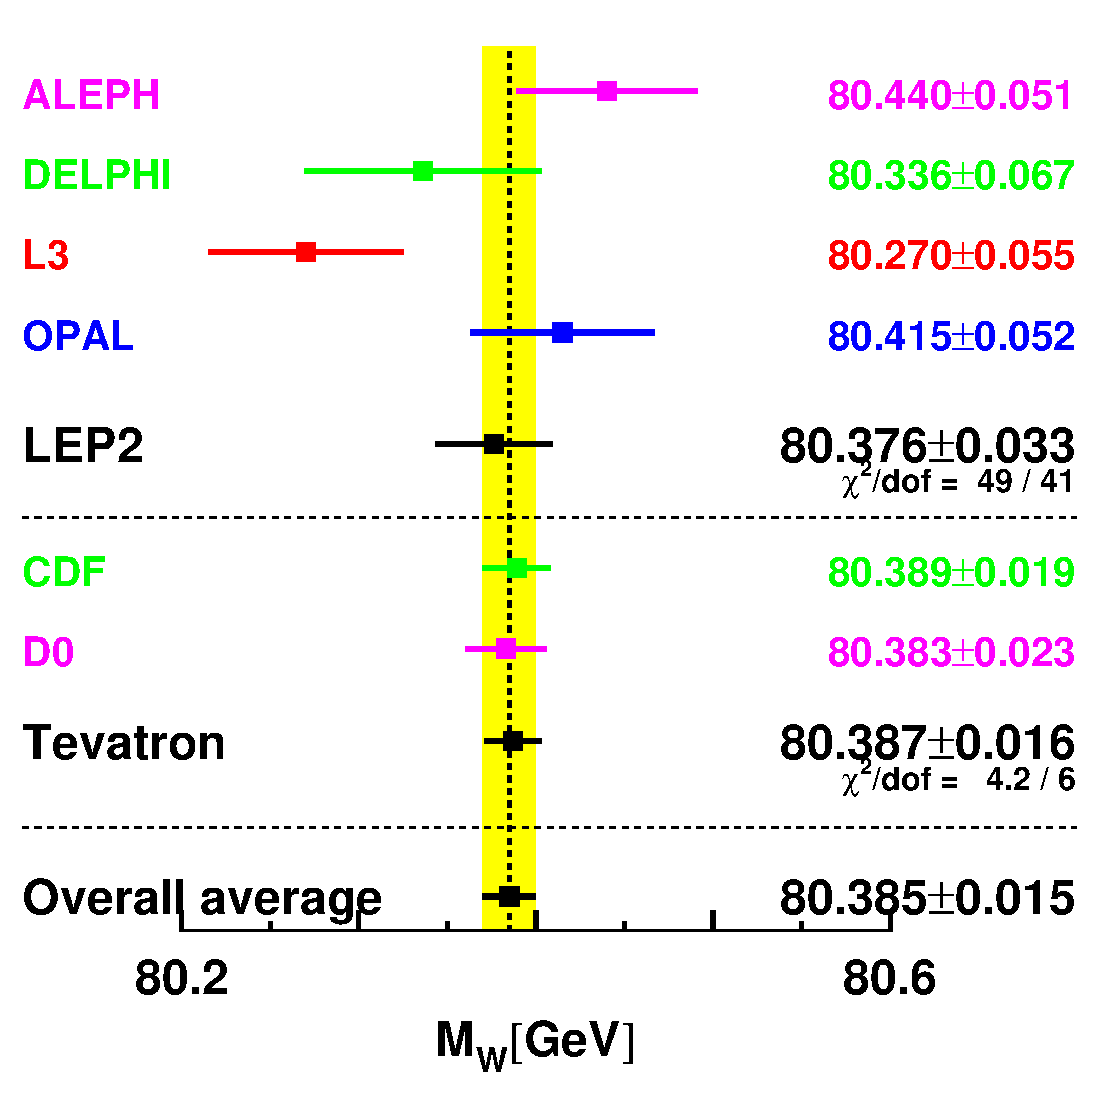
\includegraphics[width=.45\textwidth]{figures/theory/wmass_pdg.eps}
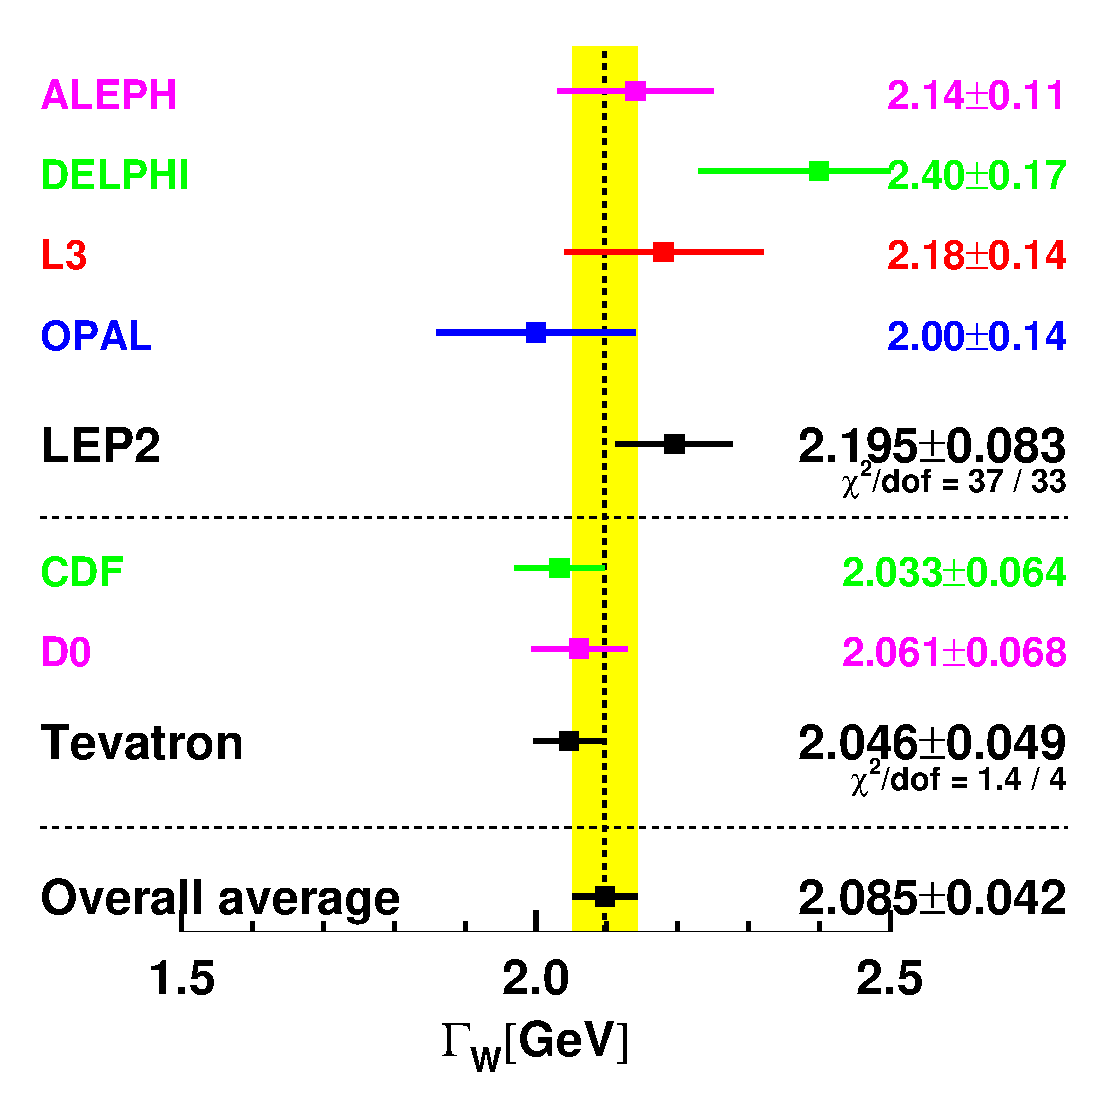
\includegraphics[width=.45\textwidth]{figures/theory/wwidth_pdg.eps}
\caption{Summary of \dubya~mass (left) and width (right) measurements
as performed at LEP and the Tevatron~\cite{PDG:2014}.}
\label{fig:theory_w_pdg}
\end{figure}


While the fundamental parameters of the EW theory are related to each other
by relations like those above, they are not determined \emph{a priori} 
and so must be first determined from experiment.
Of primary interest to the topic of this thesis 
are the measured parameters related to the behavior and properties
of the \dubya~and Higgs bosons.
The \dubya~was first discovered in 1983 via $p\overline{p}$ collisions
at the SPS by looking at its decay to an electron %abbreviation?
and electron neutrino \cite{ARNISON1983103}.
Its mass has been measured in $p\overline{p}$ collisions at the Tevatron
and in $e^{+}e^{-}$ collisions at LEP to give a world 
average of $80.385 \pm 0.015\GeV$~\cite{PDG:2014}.
A summary of the \dubya~mass measurements is shown on 
the right of \fig\ref{fig:theory_w_pdg}.
The width assuming a Breit-Wigner distribution has also been measured 
at LEP and the Tevatron as seen in the right of \fig\ref{fig:theory_w_pdg}
with an average value of $2.085\pm0.042\GeV$ \cite{PDG:2014}.
Roughly 1/3 of of the time the \dubya~decays approximately 
evenly into each of the three lepton generations,
as expected from the shared coupling of \eqn\eqref{eq:couplings_wleptons}
(ignoring kinematics).
The leptonic decays of the \dubya~result in a charged lepton 
with the same charge as the parent \dubya~(as dictated by charge conservation)
and a neutrino (or anti-neutrino if the parent \dubya~has negative charge),
as indicated in the top of \fig\ref{fig:feyn_wcoupling}.
The \dubya~decays into quarks the remaining 2/3 of the time with a positively
(negatively) charged \dubya~decaying into a up-type quark (anti-quark) 
and down-type anti-quark (quark),
like in the bottom of \fig\ref{fig:feyn_wcoupling}.
The measured branching fractions for the \dubya~are 
summarized in \tab\ref{tab:theory_wdecay}.

\begin{table}[ht]
\centering
\begin{tabular}{l|c}
Decay Mode &  Branching Fraction [\%]\\
\hline
$e^+\nu_e$ ($e^-\overline{\nu}_e$) & $10.71 \pm 0.16$ \\
$\mu^+\nu_{\mu}$ ($\mu^-\overline{\nu}_{\mu}$) & $10.63 \pm 0.15$\\
$\tau^+\nu_{\tau}$ ($\tau^-\overline{\nu}_{\tau}$) & $11.38 \pm 0.21$\\
Quarks & $67.41 \pm 0.27$\\
\end{tabular}
\caption{Measured branching fractions of the $\dubya^+$ ($\dubya^-$)~boson 
as reported by the Particle Data Group \cite{PDG:2014}.  The $W$ decays
to quarks result in hadronic states which in general prohibit
one from determining the specific $W$ final state. Thus, only 
an inclusive branching fraction is listed for the decay to quarks.}
\label{tab:theory_wdecay}
\end{table}


%The cross-section of the production of the \dubya~at colliders
%depends on the initial state (i.e. $pp$ vs $p\overline{p}$) and on the
%collision energy. 
%The cross-section times branching fraction to leptons 
%has been measured thoroughly, with separate measurements performed
%at RHIC~\cite{PhysRevLett.106.062001};
%the SPS~\cite{Albajar1987271,Alitti1992365};
%the Tevatron~\cite{0954-3899-34-12-001,D0-4403-CONF};
%and most recently at the LHC 
%at 7~\TeV~\cite{PhysRevD.85.072004,Chatrchyan:1370079}, 
%8~\TeV~\cite{PhysRevLett.112.191802}, 
%and 13~\TeV~\cite{ATLAS-CONF-2015-039,CMS-PAS-SMP-15-004}. 
%A summary of these measurements is shown in 
%\fig\ref{fig:theory_wxsec} which reveals them to be in good agreement with 
%the predictions.

%\begin{figure}[ht]
%\centering
%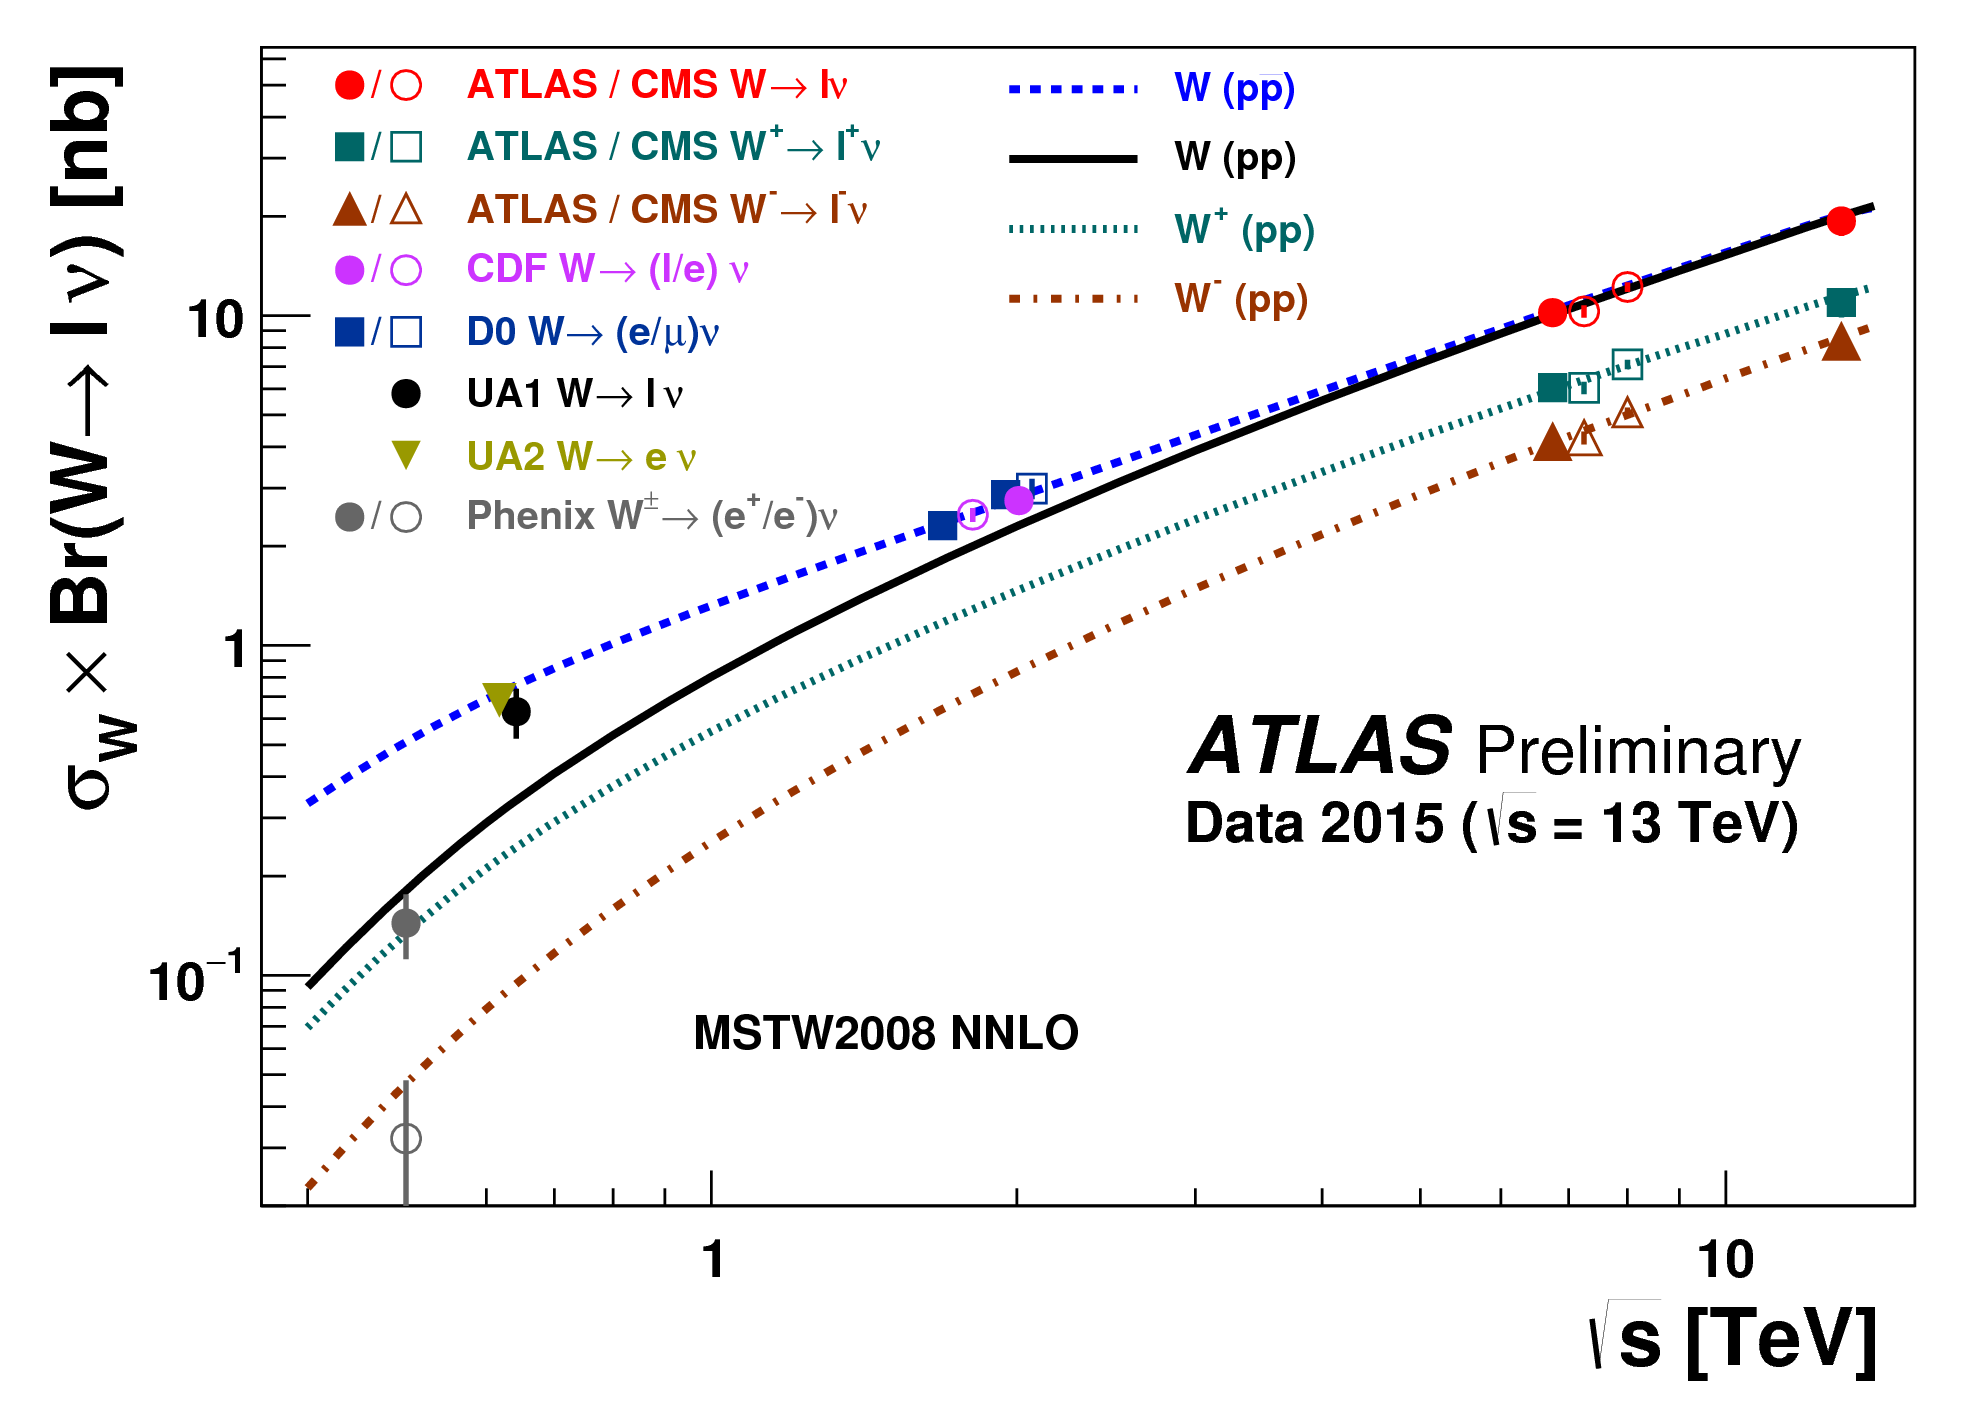
\includegraphics[width=.8\textwidth]{figures/theory/wxsec.png}
%\caption{Summary of $W\rightarrow l\nu$ cross-section measurements as 
%a function of center-of-mass energy, $\sqrt{s}$. 
%Next-to-next-to-leading-order (NNLO) theoretical
%predictions are shown for both $pp$ and 
%$p\overline{p}$ collisions and for $pp$ collisions when split by charge.
%Experimental measurements are overlayed and taken from measurements
%at the SPS, RHIC, the Tevatron, and the LHC.  The plot is taken
%from the ATLAS publication of $W$ and $Z$ cross-section measurements
%at the LHC \cite{ATLAS-CONF-2015-039}.  }
%\label{fig:theory_wxsec}
%\end{figure}

The Higgs boson was discovered in 2012 at the LHC
jointly by ATLAS \cite{Aad20121} and CMS \cite{Chatrchyan:2012xdj}.
Combined measurements of the mass between the two experiments 
show the current value of the Higgs mass to be 
$m_H = 125.09 \pm 0.21 (\textrm{Stat.}) \pm 0.11 (\textrm{Syst.})\GeV$
\cite{Aad:2015zhl} as seen in \fig\ref{fig:higgs_mass}.
Detailed studies of the spin \cite{Aad2013120,Khachatryan:2014kca},
width \cite{Aad:2015xua,Khachatryan:2014iha},
and couplings \cite{ATLAS-CONF-2015-044} are all consistent
with the Higgs boson of the SM.

\begin{figure}
\centering
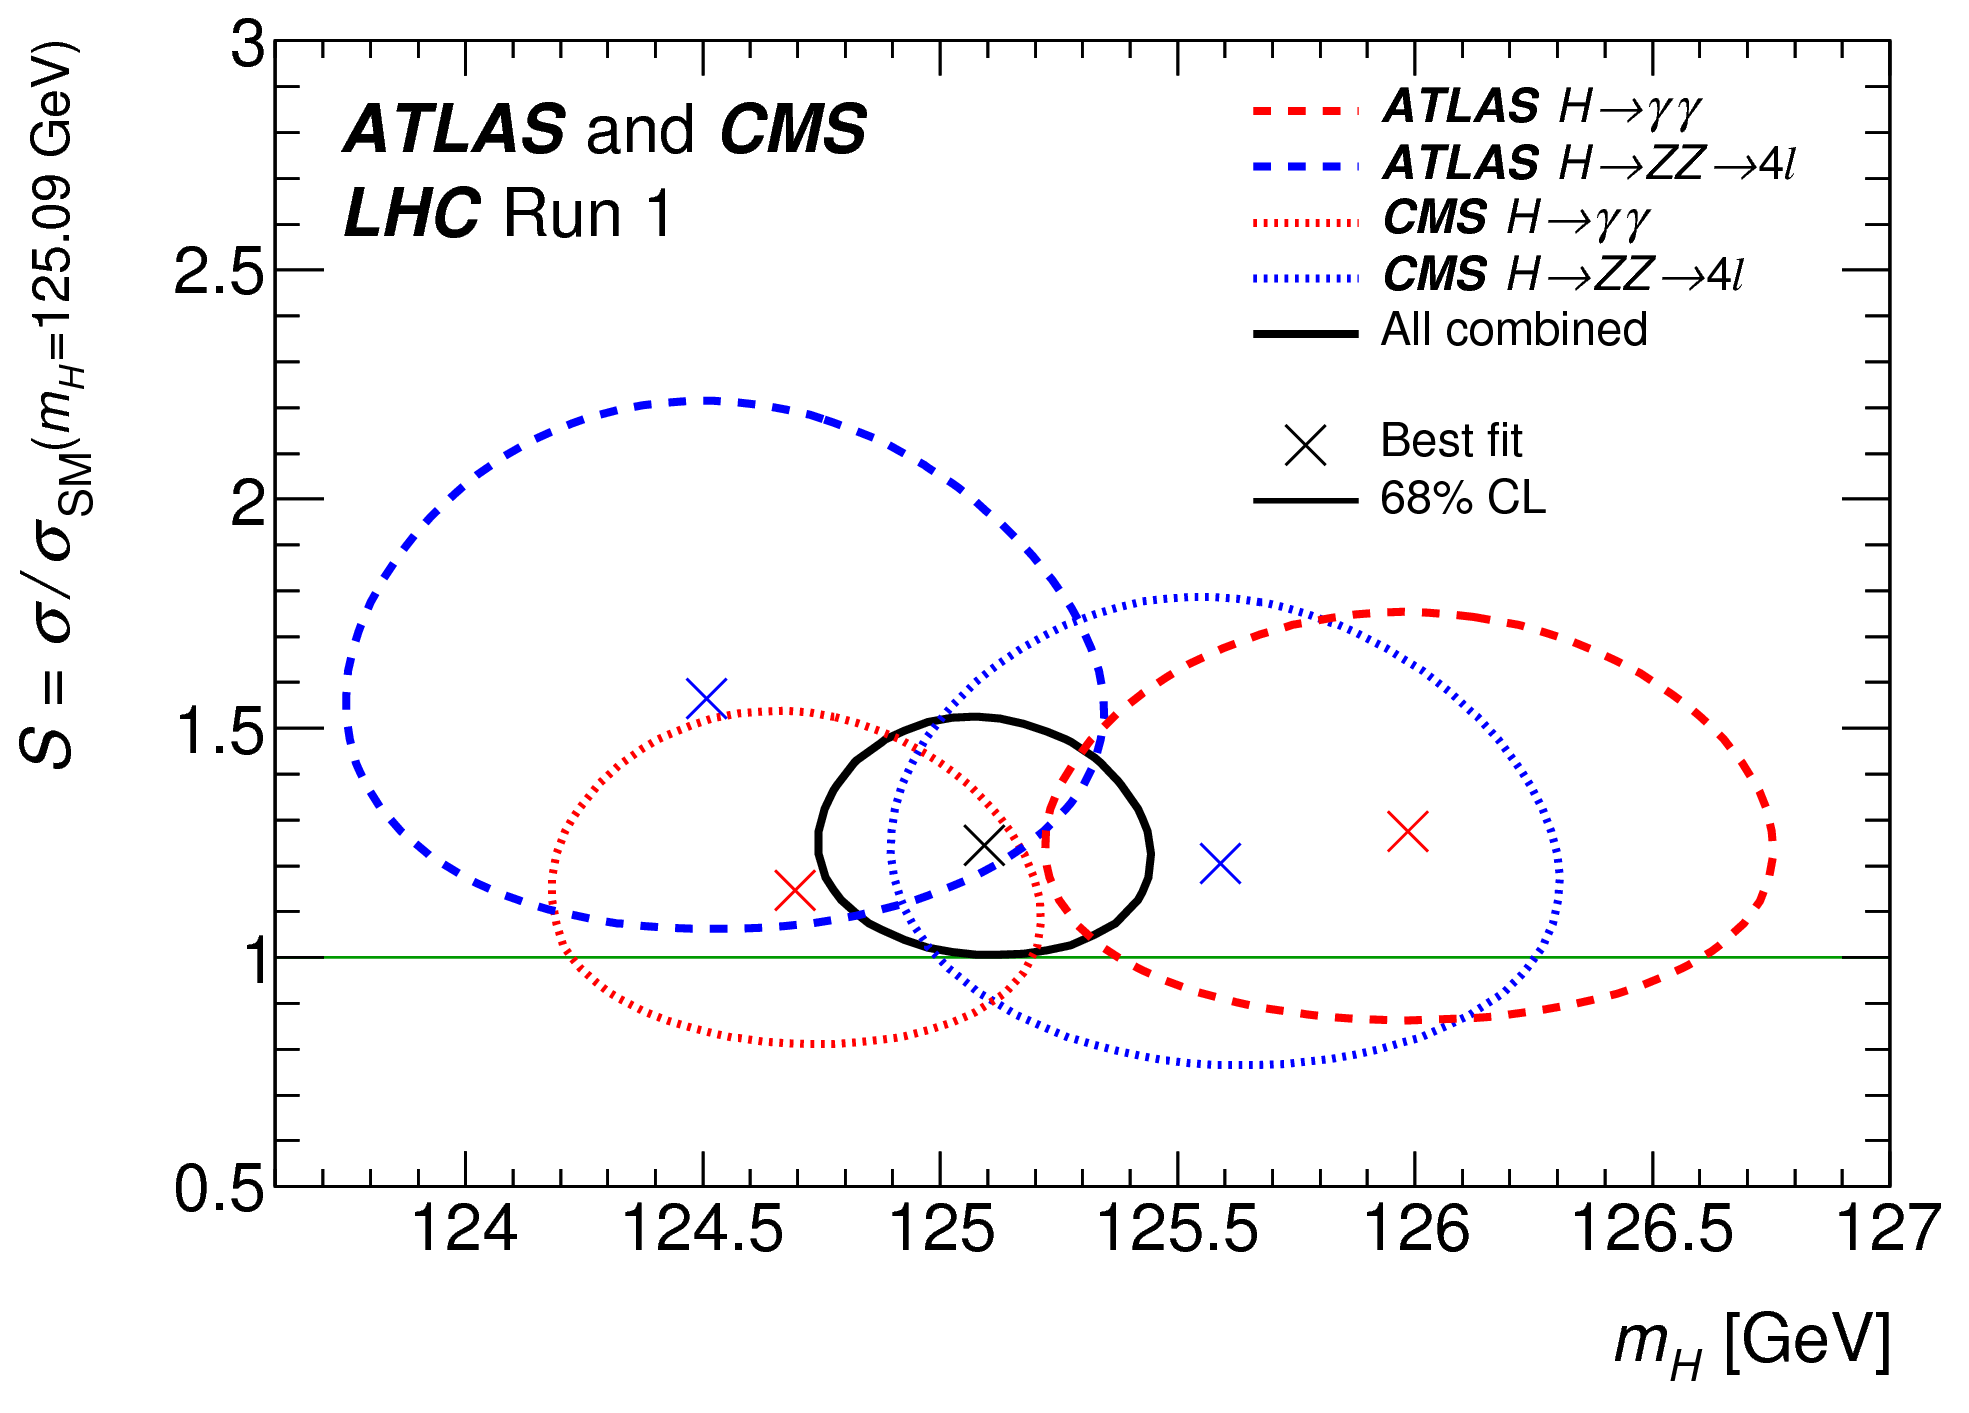
\includegraphics[width=.8\textwidth]{figures/theory/higgs_mass.png}
\caption{Combined ATLAS and CMS 
measurements of Higgs signal strength
vs mass in $H\rightarrow \gamma \gamma$ and $H\rightarrow ZZ\rightarrow 4l$
channels with 68\%CL likelihood curves \cite{Aad:2015zhl}.}
\label{fig:higgs_mass}
\end{figure}

\section{$WWW$ Production}

\unitlength = 0.6mm %necessary for feynmp
\begin{figure}[ht]
\centering
\vspace{5 mm}
\begin{fmffile}{feynwwwprod1}
		\begin{fmfgraph*}(80,50)
			\fmfleft{i1,i2}
			\fmfright{o1,o2,o3}

			\fmf{fermion}{i1,v1}
			\fmf{fermion}{v1,i2}
			\fmf{photon}{v1,v2}
			\fmf{photon}{v2,o1}
			\fmf{photon}{v2,o2}
			\fmf{photon}{v2,o3}
		\end{fmfgraph*}
\end{fmffile}
\hspace{6 mm}
\begin{fmffile}{feynwwwprod2}
		\begin{fmfgraph*}(80,50)
			\fmfleft{i1,i2}
			\fmfright{o1,o2,o3}

			\fmf{fermion}{i1,v1}
			\fmf{fermion}{v1,i2}
			\fmf{photon}{v1,v2}
			\fmf{photon}{v2,o1}
			\fmf{dashes,label=$H^0$}{v2,v3}
			\fmf{photon}{v3,o2}
			\fmf{photon}{v3,o3}
		\end{fmfgraph*}
\end{fmffile}

\vspace{6 mm}
\begin{fmffile}{feynwwwprod3}
		\begin{fmfgraph*}(80,50)
			\fmfleft{i1,i2}
			\fmfright{o1,o2,o3}

			\fmf{fermion}{i1,v1}
			\fmf{fermion}{v1,v2}
			\fmf{fermion}{v2,v3}
			\fmf{fermion}{v3,i2}
			\fmf{photon}{v1,o1}
			\fmf{photon}{v2,o2}
			\fmf{photon}{v3,o3}
		\end{fmfgraph*}
\end{fmffile}
\hspace{6 mm}
\begin{fmffile}{feynwwwprod4}
		\begin{fmfgraph*}(80,50)
			\fmfleft{i1,i2}
			\fmfright{o1,o2,o3}
			\fmf{fermion}{i1,v1}
			\fmf{fermion}{v1,v2}
			\fmf{fermion}{v2,i2}
			\fmf{photon,label=$Z/\gamma^{*}$}{v2,v3}
			\fmf{photon}{v1,o1}
			\fmf{photon}{v3,o2}
			\fmf{photon}{v3,o3}
		\end{fmfgraph*}
\end{fmffile}
\vspace{2 mm}
\caption{The tree level Feynman diagrams 
for $WWW$ production. The incoming fermion
lines in each diagram consist of an
up-type quark (anti-quark) and down-type anti-quark (quark). Unless
otherwise specified, the curved lines correspond to $W$ bosons.}
\label{fig:theory_feynman_www}
\end{figure}

In this thesis, we are interested in the inclusive production of three
$W$ bosons from proton-proton collisions:
$pp\rightarrow\- \Wp\Wp\Wm+X$ and $pp\rightarrow \Wp\Wm\Wm\allowbreak +X$, 
where $X$ is intended to refer to the fact that no requirements are 
placed on additional particles produced in the hard interaction.
This is sensitive both
to the $WWWW$ coupling (non-resonant production) 
and to associated Higgs production \footnote{Associated Higgs production involves
the radiation of a Higgs boson off another particle (in this case a $W$ boson). It 
is sometimes referred to as ``Higgsstrahlung'', by analogy 
with electron Bremsstrahlung where an electron radiates a photon.} where 
the Higgs decays to two
$W$ bosons (resonant production). 
The relevant
tree-level Feynman diagrams for this production process are shown in 
\fig\ref{fig:theory_feynman_www}.
The Higgs decay results in one $W$ boson being produced off-shell,
$H\rightarrow WW^*$, making this the leading contribution to off-shell
production.  
The resonance from the Higgs can clearly be seen from the 
distribution of $m_{\Wp\Wm}$ taken from the simulation of production \www~events
in \fig\ref{fig:mww_higgs}.

%It would be nice to show a plot of the Higgs stuff. maybe I can
%steal this and make my own later...
\begin{figure}[ht]
\centering
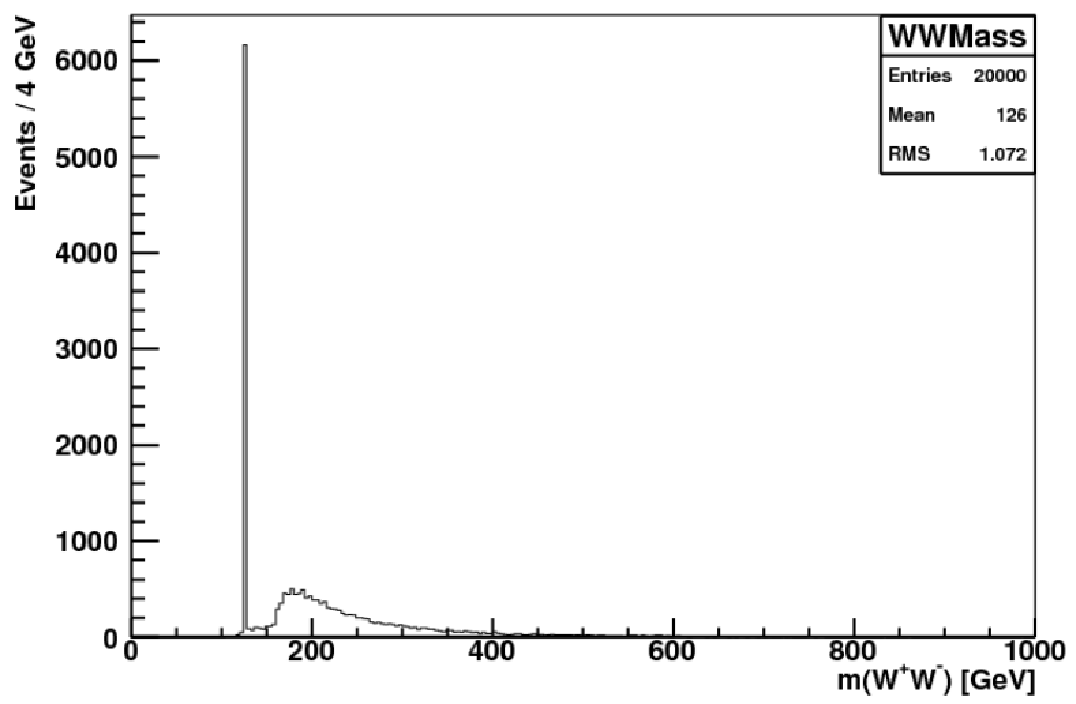
\includegraphics[width=0.5\columnwidth]{figures/2l2j/mWW-parton.pdf}
\caption{ Invariant mass distribution of two opposite-sign $W$ bosons 
in \www events generated with VBFNLO at LO. The Higgs mass peak is clearly 
visible at 126~GeV. (make a better plot)}
\label{fig:mww_higgs}
\end{figure}




The cross-section for this process can be computed at 
next-to-leading-order (NLO) in QCD
( $O(\alpha_s^2)$ in perturbation theory (?) ). 
(Mention more details of how this is computed like PDFs,
hadronization, interaction, radiation, decays. Use one of the 
Feynman diagrams)
Using 
the \madgraph~generator finds an inclusive cross-section of 
\begin{equation}
\sigma(pp\rightarrow WWW + X) = 241.47 \pm 0.13~\textrm{fb}
\label{eq:www_total_xsec}
\end{equation}
where the uncertainty is purely statistical.
The contribution from resonant production is computed separately
and found to make up about 64\% of the 
total inclusive cross-section.
More details on the determination of the signal cross-section, uncertainties,
and kinematics are presented in \sec\ref{sec:signal}.

\begin{figure}
\centering
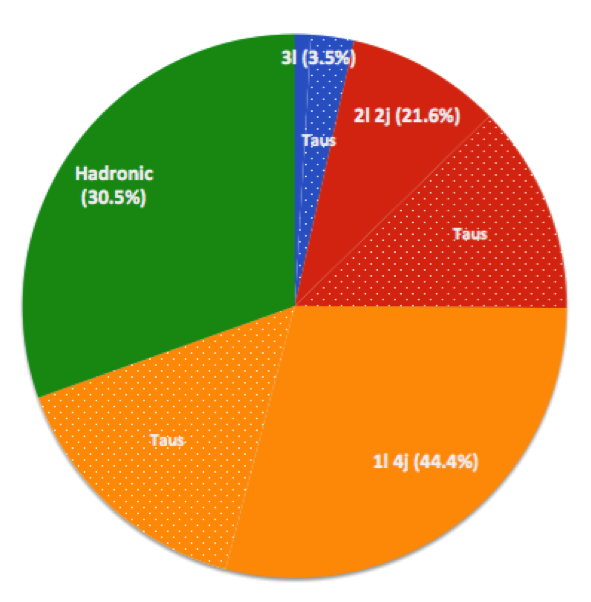
\includegraphics[scale=.8]{figures/branching_fractions.png}
\caption{Pie chart showing the different decay modes contributing 
to the total \xsec for the \www~process. 
The dotted areas indicate the portion of each decay 
mode which is due to the production of tau leptons.}
\label{fig:branching_fractions}
\end{figure}

Due to the short lifetime of the $W$ boson, each of the $W$ bosons
in the $WWW$ process will decay before reaching the detector.
This results in a measurable final state for the $WWW$ production 
process that includes some combination of leptons 
and quarks (manifested as jets).  The branching fractions for 
the $WWW$ process can be determined from the individual $W$ branching fractions
listed in \tab\ref{tab:theory_wdecay}.  The expected $WWW$ branching
fractions are thus summarized in the pie chart in \fig\ref{fig:branching_fractions}.
For this thesis, we are primarily interested in the final state
where each $W$ boson decays leptonically (the fully-leptonic final state) 
which has the smallest branching fraction at roughly 3.5\%.
In fact, since the $\tau$ leptons are also unstable, we choose to 
omit $W$ decays to $\tau$ leptons from our fully-leptonic
definition as well. This further reduces the fully-leptonic 
branching fraction to 0.97\%.  While small, this fully-leptonic final state
should have smaller backgrounds to the signal than the other 
decay channels, making it one of the most sensitive channels for studying
this process. The branching fraction when one $W$ boson is allowed
to decay hadronically is considerably larger, at 21.6\% (or
9.2\% when excluding decays to $\tau$ leptons). This is 
referred to as the semi-leptonic decay channel. The presence
of the two leptons from the other two $W$ decays still allows
for background discrimination, though not as much as in the fully-leptonic
channel. As a result, this channel has also been studied, though it 
is not the focus of this thesis. The remaining channels have
not been studied. The combination of the fully-leptonic
and semi-leptonic channels is presented in \sec\ref{sec:measurement}.



\section{Effective Field Theory}

The lagrangian of the SM, summarized by 
\eqn\eqref{eq:lagrangian_sm},~\eqref{eq:lagrangian_qcd},
~\eqref{eq:lagrangian_ew}, and~\eqref{eq:lagrangian_ewsb}
has so far been very successful. 
But, as we continue to probe higher energy scales, 
there is reason to believe that the SM's luck will run out.
If history is any guide, the SM is simply
an approximation of a larger theory whose details are not relevant
relevant at current energies.
Indeed, the SM leaves important questions unanswered (for example, 
the hierarchy problem) that could be explained
by the observation of some new high energy phenomena.  %more detail

This idea of the SM as an approximate theory
can be made explicit 
using an Effective Field Theory (EFT) \cite{Pich:1998xt}
approach which includes new terms in the lagrangian, in addition to the SM.
As a function of the energy, these terms start small 
but become increasingly important at higher and higher energies.
In general, the new EFT terms might look like this:
\begin{equation}
\curlyl_{\textrm{EFT}} = \curlyl_{\textrm{SM}} + \sum_{n=5}^{\infty} \sum_i \frac{c_{n,i}}{\Lambda^{n-4}} \curlyo_{n,i}
\end{equation}
where $\Lambda$ is some new energy scale relevant to the new
physics we seek to describe and the $c_{n,i}$ are dimensionless
couplings.  While the operators of the SM have mass dimension 4, the EFT 
operators, $\curlyo_{n,i}$, have a mass dimension
$n>4$ which describe the new interactions between the SM fields at low energy
due to the new physics model.
The sum over $i$ is simply to indicate that there are in general multiple 
possible new operators for a given mass dimension.
These EFT operators come from ``integrating out'' the high energy interactions
between the SM fields and the fields in the new physics model,
leaving behind contact interactions between the SM fields and factors
of $\Lambda^{n-4}$ in the denominator.
These factors of $\Lambda$ suppress the new terms
with respect to the SM, with the suppression becoming stronger as $n$ grows.
Thus, only the first terms in the summation
over $n$ are important at low energy.

The list of possible gauge-invariant EFT operators to 
consider is long \cite{Hagiwara:1993ck,Buchmuller:1985jz,Eboli:2006wa}
One way to shorten the list is to impose certain symmetries. 
Enforcing the conservation
of baryon and lepton number restricts 
us to only even values of $n$:
\begin{equation}
\curlyl_{\textrm{EFT}} = \curlyl_{\textrm{SM}} + \sum_i \frac{c_{6,i}}{\Lambda^2} \curlyo_{6,i} + \sum_j \frac{c_{8,j}}{\Lambda^4} \curlyo_{8,j} + \dots
\label{eq:lagrangian_eft}
\end{equation}
where we have truncated the series at $n=8$ since these
these higher order terms are small.
The leading $n=6$ terms predict new anomalous triple and quartic 
gauge coupling (aTGC and aQGC) interactions while the sub-leading $n=8$ terms
predict only new aQGC interactions. 
Predictions of aTGC interactions have been studied in detail at 
LEP, the Tevatron, and the LHC  with no luck \cite{PDG:2014}.
But there is still hope!
It could be that new physics is suppressed in aTGC interactions
but not in aQGC interactions. \footnote{For instance, the aTGC interactions
could first appear at the one loop level while the aQGC 
interactions appear at tree level.}
Then the new physics might first appear at $n=8$, where only aQGC interactions
occur.



%\subsection{Anomalous Quartic Gauge Couplings}

In a linear EFT model where the Higgs field is indeed the mechanism for EWSB, 
the possible $n=8$ operators 
in \eqn\eqref{eq:lagrangian_eft} can
be split into three categories: those containing covariant derivatives,
as in \eqn\eqref{eq:ew_covariant_derivative}, of the Higgs field, $\phi$; 
those containing covariant derivatives of the Higgs field and 
the field strength tensors, as 
in \eqn\eqref{eq:wfieldstrength} and \eqref{eq:bfieldstrength};
or those containing only field strength tensors \cite{Eboli:2006wa,Eboli:2003nq}. 
All of these operators preserve CP symmetry.
In this thesis, we are
interested only in the first category, which is limited to just two operators:
\begin{align}
\curlyo_{S,0} =& \Big[(D_{\mu}\phi)^{\dagger} D_{\nu} \phi\Big] \times \Big[(D^{\mu} \phi)^{\dagger} D^{\nu} \phi \Big] \\
\curlyo_{S,1} =& \Big[(D_{\mu}\phi)^{\dagger} D^{\mu} \phi\Big] \times \Big[(D_{\nu} \phi)^{\dagger} D^{\nu} \phi \Big]
\end{align}
which could come from integrating out some new 
vector gauge boson resonance coupling to the EW gauge bosons \cite{Baak:2013fwa}.
Plugging these into \eqn\eqref{eq:lagrangian_eft} (and dropping all other terms
besides the SM), we get
\begin{equation}
\begin{aligned}
\curlyl_{\textrm{EFT}} = \curlyl_{\textrm{SM}} +&
\frac{f_{S,0}}{\Lambda^4}\Big[(D_{\mu}\phi)^{\dagger} D_{\nu} \phi\Big] \times \Big[(D^{\mu} \phi)^{\dagger} D^{\nu} \phi \Big] \\
+& \frac{f_{S,1}}{\Lambda^4}\Big[(D_{\mu}\phi)^{\dagger} D^{\mu} \phi\Big] \times \Big[(D_{\nu} \phi)^{\dagger} D^{\nu} \phi \Big]
\end{aligned}
\label{eq:lagrangian_aqgc}
\end{equation}
where we have introduced the new arbitrary couplings $f_{S,0}$ and $f_{S,1}$.
Expanding this out we get...
These modify the SM QGC interactions of \eqn\eqref{eq:lagrangian_qgc}
and \fig\ref{fig:theory_feynman_couplings_qgc}
to produce new aQGC interactions $W^+W^-W^+W^-$, $W^+W^-ZZ$, and $ZZZZ$
that do not depend on the gauge boson momenta (do I care?).
In this thesis, we are interested only in the aQGC
interaction term involving $W^+W^-W^+W^-$, which predicts  
a new tree level diagram for the $WWW$ production process similar to the SM QGC
production of this process in \fig\ref{fig:theory_feynman_couplings_qgc}.
If real, such a modification would enhance the predicted 
cross-section in \eqn\eqref{eq:www_total_xsec}.

By definition, the EFT approach is expected to break for energies
greater than $\Lambda$. Thus the issue arises of what energy 
$\Lambda$ corresponds to.

Unitarity...
not UV complete
effective lagrangian (could be used elsewhere to refer to the eft lagrangian)
the effect from unitarity violation typically sets in earlier due to the higher exponent in Lambda in the denominator. 

Unitarity violation is somehow related to how we can choose Lambda


\section{Status of QGC Measurements and aQGC Limits}
A variety of measurements sensitive QGC interactions have been
performed at colliders. In particular, measurements sensitive
to $WW\gamma\gamma$ have been performed 
at LEP \cite{Abdallah:2003xn,PhysRevD.70.032005}, 
the Tevatron \cite{PhysRevD.88.012005}, %is this really the only Tevatron measurement??
and the LHC \cite{PhysRevLett.115.031802,PhysRevD.90.032008,Chatrchyan:2013akv}; 
%mention how they were probed?
to $WWZ\gamma$ at LEP~\cite{Achard:2001eg,Abbiendi:1999aa,Abbiendi:2003jh}
and at the LHC~\cite{PhysRevD.90.032008};
to $ZZ\gamma\gamma$ at LEP \cite{Achard:2002iz,PhysRevD.70.032005}; 
and to $WWWW$ at the LHC \cite{PhysRevLett.113.141803,PhysRevLett.114.051801}. 
%Typically, these studies are performed
%by looking at x final state (more detail). 
%The first measurements sensitive to the $WWWW$ vertex focused on 
%same-sign $WW$ vector boson scattering because...

%material on limits?

%summary plots? maybe from PDG?

More details?





%No more than a few pages
%Include:
%- General features of the LHC and the injector chain
%- Luminosity and integrated luminosity
%- could discuss the details of the accelerator and machine parameters


%define these abbreviations here:
%LHC - Large Hadron Collider
The Large Hadron Collider (LHC) \cite{lhc} is
a 27 km circumference collider ring
located at CERN approximately 100 m underground on the 
of French-Swiss border near Geneva, Switzerland.
Its primary goal is to collide protons at energies on the TeV scale, 
energies that are so large they can replicate conditions just moments
after the big bang.
The products of these collisions can 
be observed
by several independent but complementary detectors placed at different
points around the ring in order to discover the mechanism
for EWSB as well as possible new physics processes beyond the SM.
Since the dynamics of the collisions are governed by quantum mechanical
processes, the types of processes of interest cannot be
produced on demand, but instead occur at random with some
probability.
The probabilities for these physics processes are 
typically very small and are thus quite
rare \footnote{ATLAS has been able to measure cross-sections as 
low as about 1 fb \cite{PhysRevLett.113.141803}, which is roughly
14 orders of magnitude below the measured inclusive cross-section
at the LHC \cite{Aad:2014dca}.}.
Also, these physics processes do not live long
enough to reach the detector and are instead observed indirectly through their
decays. Since multiple physics processes can have the same decay 
signature, it is not possible to say with certainty that a given 
collision comes from a specific physics process. Instead, 
we must count the number of observed collisions for a given signature
and compare this to the number expected from the 
quantum mechanical probabilities provided by cross-section
calculations.  If the observed number differs
from the expected, then it could simply suggest that the theoretical expectation
is not well understood.  Or, it could suggest the presence of some new physics
process beyond the SM.
In order to make an adequate statement, we must be able to count
enough collisions of the desired signature 
such that the statistical uncertainty is low
(say 10 to 1000 depending on the signature and its backgrounds).  
This places a demand
on the LHC to produce as many collisions as possible, even of these rare
processes. To accomplish this, the LHC is designed to collide
protons at a maximum frequency of 400 MHz, or 400 million times per second!
More details about the LHC and collider physics in general are presented
below.



\section{Collider Physics}
\label{sec:lhc_collider_physics}

From the perspective
of a particle physicist studying the products of particle collisions, we 
are interested in collisions produced at the highest possible energies,
measured by the collision center-of-mass energy, and at the highest possible rates, 
measured by the luminosity.
The center-of-mass energy, $E_{\textrm{CM}}$, is the collision energy 
in the rest frame
of the collision. For head-on collisions with both beams at the same
energy, $E$, like at the LHC, this is simply the sum of the energies, 
or $E_{CM} = 2 E$. So, $E_{\textrm{CM}}$ grows linearly as a function
of the beam energy. This is in contrast with fixed target experiments
where $E_{\textrm{CM}} \propto \sqrt{E}$ and thus grows much more slowly. 
Frequently this is related to the Mandelstam variable,
$s$, which is the squared magnitude of the Lorentz four-vectors
of the incoming collision particles $p_1$ and $p_2$, such that
$s = (p_1+p_2)^2 = E_\textrm{CM}^2$.
The high beam energies required prefer a circular collider (as opposed
to a linear collider) so that the particles may be repeatedly 
accelerated at each cycle using the same hardware.
In order to accelerate the particles, they must be both stable (if they
are to hang around long enough to collide) and charged (so
that they may respond to electromagnetic steering and acceleration).
This leaves just protons and electrons (and their anti-particles)\footnote{It is also
possible to collide heavy ions, such as lead. In fact, the LHC does collide
heavy ions when it is not colliding protons, though that is not the focus of this
thesis.}.
To get the particles to very high energies, the particles
are ultimately accelerated using electromagnetic waves in radio-frequency cavities.
The beam is chopped up into ``bunches'' separated at regular intervals
to synchronize with and ``surf'' the wave amplitude. The frequency
of the radio-waves thus determines the bunch spacing.
To bend the particles around the ring at high beam energies 
requires tremendously strong dipole magnets. 
Thus, the limiting factor for the energy is ultimately the requirements
on the dipole magnets, which must be superconducting and at the cutting-edge 
of current technology.

Upon acceleration, these particles emit synchrotron radiation.
Too much synchrotron radiation and the beam could lose more energy
than is practical. 
Electrons and positrons are fundamental particles and thus provide
very clean collisions, but their small mass means that they suffer
from high energy losses due to synchrotron radiation.. 
This decides the overall radius and size of the collider ring, since a smaller
ring means tighter turns and thus more acceleration\footnote{In fact, 
the LHC uses the same tunnel (which was the same size) as 
the Large Electron-Positron (LEP) Collider and which
operated from 1989 to 2000 but only up to energies of 209 GeV for the reasons
described.}.
Protons and anti-protons, with their larger mass, 
are much less affected by synchrotron radiation
and thus can be accelerated to higher energies for a fixed radius 
circular collider. As a result, these are the particles used
in modern high energy colliders, with protons-antiprotons collisions
at the Tevatron and Sp$\overline{\textrm{p}}$S, and proton-proton
collisions at the LHC.


\begin{figure}[ht]
\centering
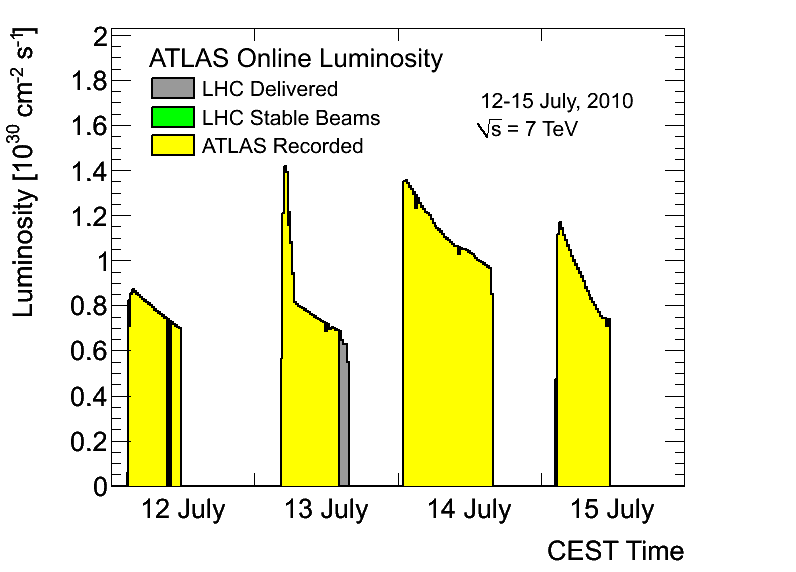
\includegraphics[width=.7\textwidth]{figures/lhc/instantaneouslumi.png}
\caption{Instantaneous luminosity as a function of time
as recorded by ATLAS for several runs in 2010.}
\label{fig:lhc_inst_lumi}
\end{figure}

The luminosity, $L$,  can be thought of as the overall intensity of the beam.
For a colliding beam it may be simply defined as
\begin{equation}
L=f \frac{N_b^2}{4\pi\sigma^2} R
\end{equation}
where $f$ is the collision frequency (related to the bunch spacing and thus
in the MHz radio-frequency range), 
$N_b$ is the number of particles in a bunch (usually 10-100 billion), 
$R$ is a  geometrical factor
taking into account details like the crossing angle of the collision (on the
order of unity),
and $\sigma$ is the transverse size of the bunches\footnote{Not to be confused
with the cross-section in particle physics.} (which 
is usually on the order of tens of microns).
Thus, modern colliders typically have luminosities on the order of 
$10^{30}$ to $10^{34}~\lumiunits$ \cite{PDG:2014}.
The transverse size of the beam is governed by the relativistic 
energy of the beam and is carefully tuned in the LHC
using arrays of focusing magnets. 
The luminosity of the beam is not constant, but instead steadily decreases
exponentially as a function of time, $t$:
\begin{equation}
L(t) = L_0 e^{-t/\tau_L} 
\label{eq:lhc_lumi}
\end{equation}
where $L_0$ is the initial luminosity and $\tau_L$ is the lifetime of the 
beam. The finite lifetime (on the order of hours) comes from gradual 
degradation of the beam quality, mainly due to the beam collisions themselves.
As the beam reaches the end of its 
life (usually 1/4 to 1/2 of the peak luminosity), the beam is dumped and a new
run is started. This process is repeated as many times as possible. 
An example of the instantaneous luminosity in ATLAS can be seen for
several runs in 2010 in \fig\ref{fig:lhc_inst_lumi}.
The luminosity is then integrated over time as a measure of how many collisions
were performed (and also how much data was collected).  This can
then be related to the cross-section for a given process, $\sigma$, to estimate
how many events from that process, $N$, would have been produced on average:
\begin{equation}
N=\sigma \int L~ \textrm{d}t
\label{eq:lhc_nevents}
\end{equation}

\begin{figure}[ht!]
\centering
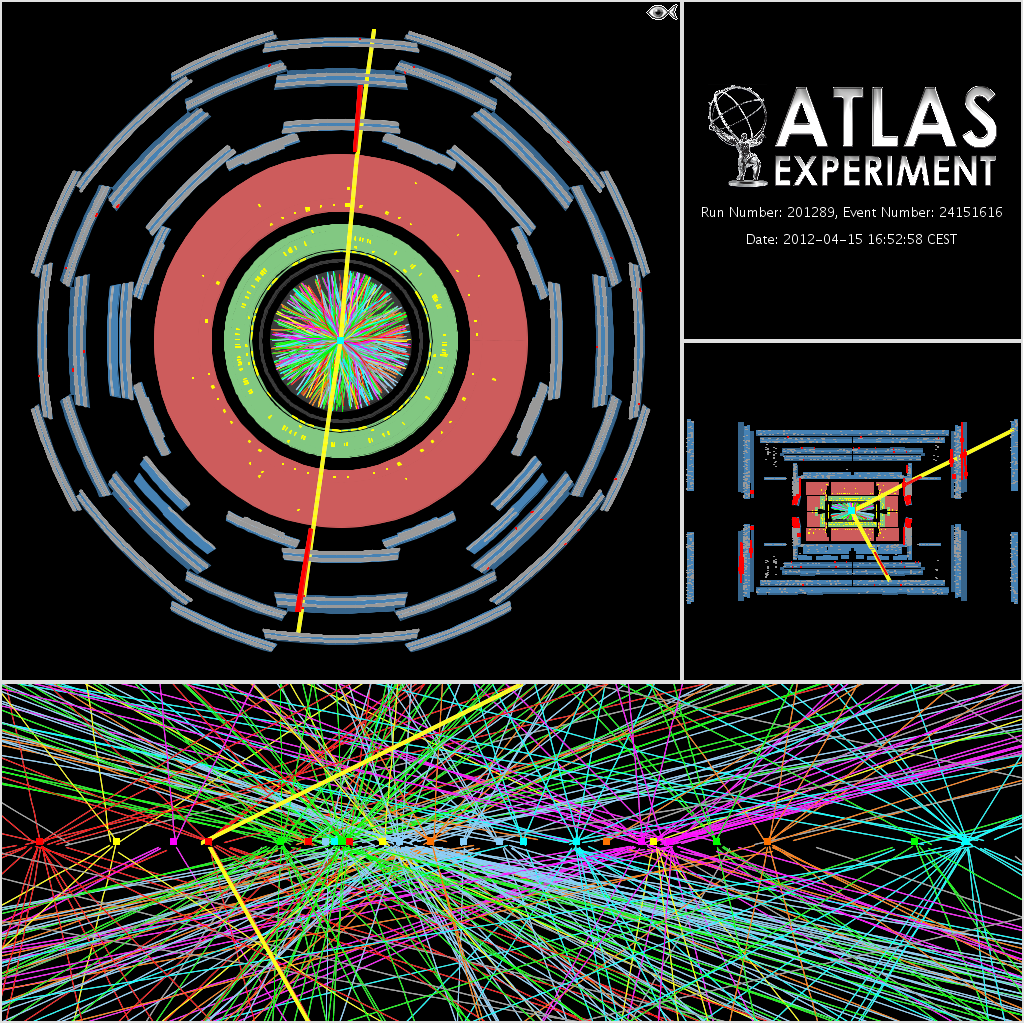
\includegraphics[width=.8\textwidth]{figures/lhc/pileup_vertexing.png}
\caption{An event display 20 pileup interactions in a single bunch crossing. 
The resulting tracks are shown, along with two high energy muons extrapolated back
to a single primary vertex. The upper left shows a cross-section of the whole
detector in the transverse plane, the upper right shows
the detector viewed along the $r-z$ plane, and 
the bottom portion is zoomed in to the length of the bunch crossing. 
The average bunch crossing length at the LHC is around 10 cm \cite{PDG:2014}.  }
\label{fig:lhc_pileup}
\end{figure}

While it is true that the we desire to increase the luminosity as much
as possible, there is one important subtlety. 
Limitations on the size of the luminosity do not just
come from the collider but also come from the detectors' ability to 
handle ``pileup''.
Pileup is the phenomena of multiple collisions occurring during a single
bunch crossing. Since we are trying to make statements about the 
physics of collisions, and not bunch crossings, we must be able to 
identify the individual collisions themselves. The typical length of 
a bunch is usually on the order of tens of centimeters while the number of pileup 
collisions per bunch crossing is on the order of ten or more. Furthermore, 
the collisions do not occur inside the detector. Instead, the decay products
are measured a few centimeters away, where the detector volume starts. 
Thus, to distinguish individual
collisions the detector must be able to extrapolate the tracks of the decay
products back to the collision point with a resolution much less than 
a centimeter. This process is called vertexing and places strict 
requirements on the precision of the tracking systems for any detector
built at a modern collider. An example of the vertexing challenges for a typical
bunch crossing in ATLAS is shown in \fig\ref{fig:lhc_pileup}.
Another issue of pileup is that each collision produces thousands of 
tracks which all contribute to the occupancy of the detector. If the occupancy
is saturated, the detector may not be able to resolve individual tracks
and would thus be useless. This is a serious concern for detectors
at future colliders where problems of pileup will continue to grow.


\section{The LHC Accelerator Complex}

\begin{figure}[ht]
\centering
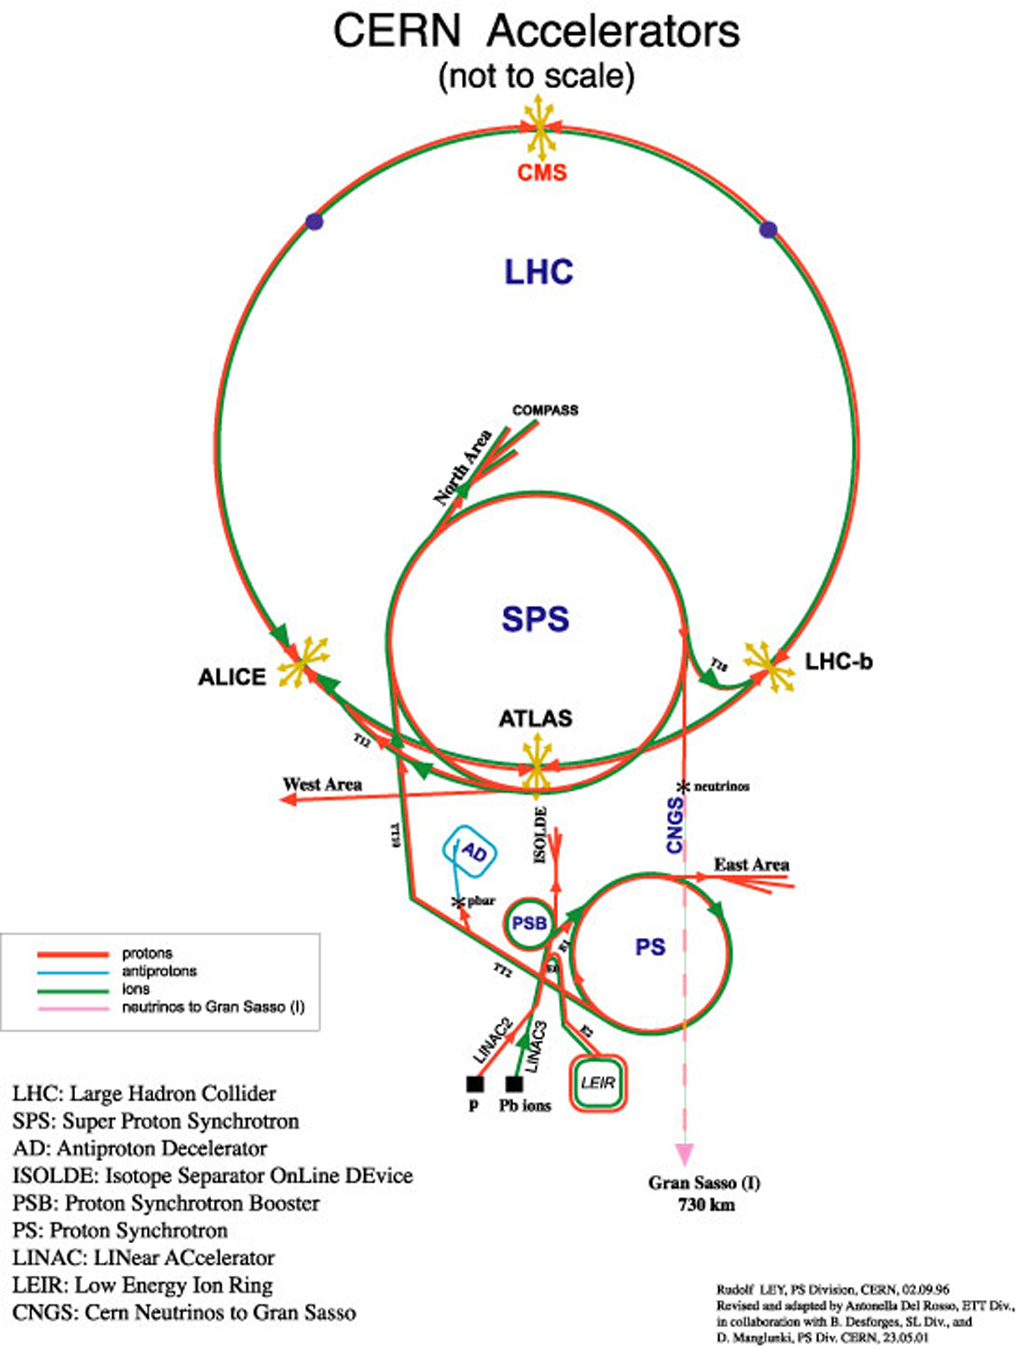
\includegraphics[width=.8\textwidth]{figures/lhc/complex.jpg}
\caption{Diagram of the different accelerators in the CERN accelerator
complex~\cite{lhccomplex}. Those relevant for the LHC are the LINAC2, 
PSB, PS, SPS, and the LHC itself. The ATLAS detector is labeled 
at the bottom of the LHC ring.}
\label{fig:lhc_complex}
\end{figure}

The LHC was designed to provide proton-proton collisions
at an energy of 14 TeV (7 TeV per beam) 
and a peak luminosity of $10^{34}~\lumiunits$ with a 25 ns collision
bunch spacing (400 MHz).
Protons are collected from hydrogen gas by first stripping away 
the electron in an electric field\footnote{Anti-protons
can be produced  from the products of 
particles collisions with a fixed target and
then trapping them using a process called stochastic cooling. This process
is much slower than the process for collecting protons. While colliding both 
protons and antiprotons increases the cross-section
for many physics processes, the high luminosity requirements on the LHC,
coupled with the relatively short luminosity lifetime, make it challenging
to do and still provide adequate integrated luminosity.}.
The protons are injected
into a series of lower energy accelerators before ultimately 
reaching the LHC to be accelerated to the full energy and 
begin collisions. The various stages of the LHC accelerator
complex are shown in \fig\ref{fig:lhc_complex}.
The protons are accelerated initially using the LINAC2 linear
accelerator. Next, the protons accelerate through the circular
Proton Synchrotron Booster (PSB), Proton Synchrotron (PS),
and Super Proton Synchrotron (SPS). Finally, they 
are split into two beams and injected into the LHC
traveling in opposite directions. Once in the LHC
ring they are accelerated to their full energy and then made
to collide at four points along the ring where detectors
are positioned to examine the products of the collisions.
The two general purpose detectors, ATLAS \cite{ATLAS} and CMS \cite{CMS}, 
are positioned at opposite sides of the ring. 
Meanwhile, the two specialized detectors, ALICE \cite{ALICE} 
and LHC-b \cite{LHCB}, are situated at equal points along the ring
nearest ATLAS.
The total injection process takes about 4 minutes.




\section{Data Collection}

\begin{figure}[ht]
\centering
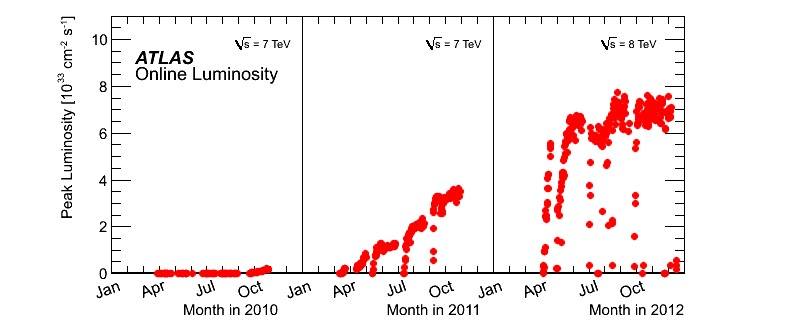
\includegraphics[width=.9\textwidth]{figures/lhc/peaklumi_multiyear.png}
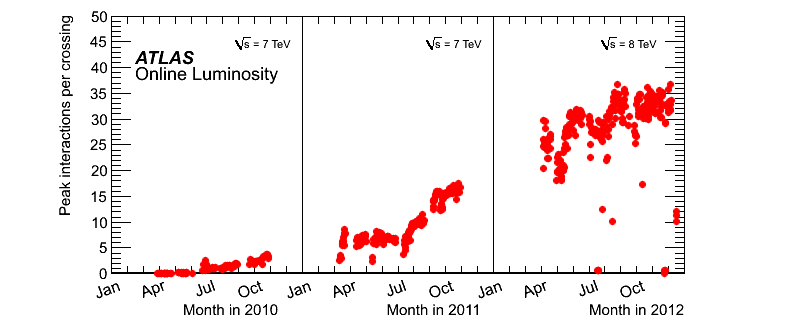
\includegraphics[width=.9\textwidth]{figures/lhc/peakmu_multiyear.png}
\caption{ (Top) The peak luminosity from the LHC as a function of time
for 2010, 2011, and 2012 data-taking periods and (Bottom)
the peak number of pileup interactions as a function of time
as recorded by ATLAS. The peak luminosity and pileup interactions
have both increased since the LHC began operation in 2010.
The gaps in recorded values are due to technical stops and long shutdowns
for maintenance and upgrade work.  }
\label{fig:lhc_conditions}
\end{figure}

\begin{figure}[ht]
\centering
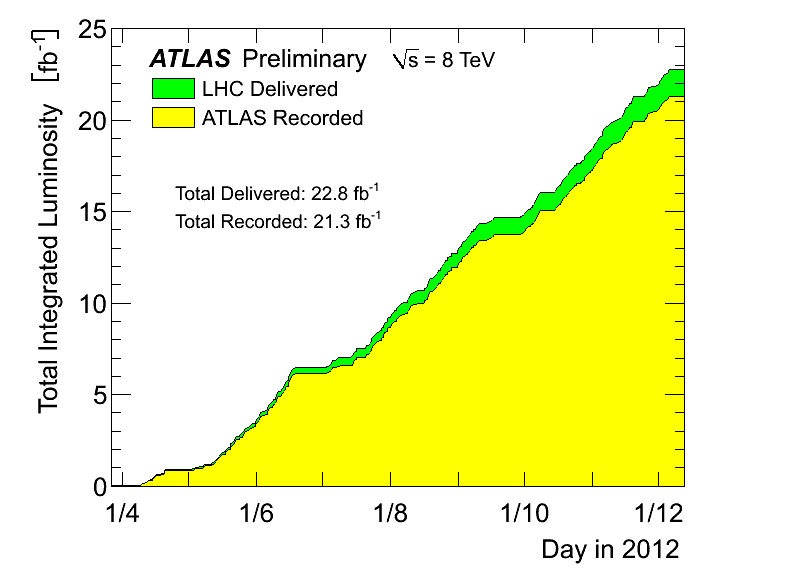
\includegraphics[width=.45\textwidth]{figures/lhc/integratedlumi.png}
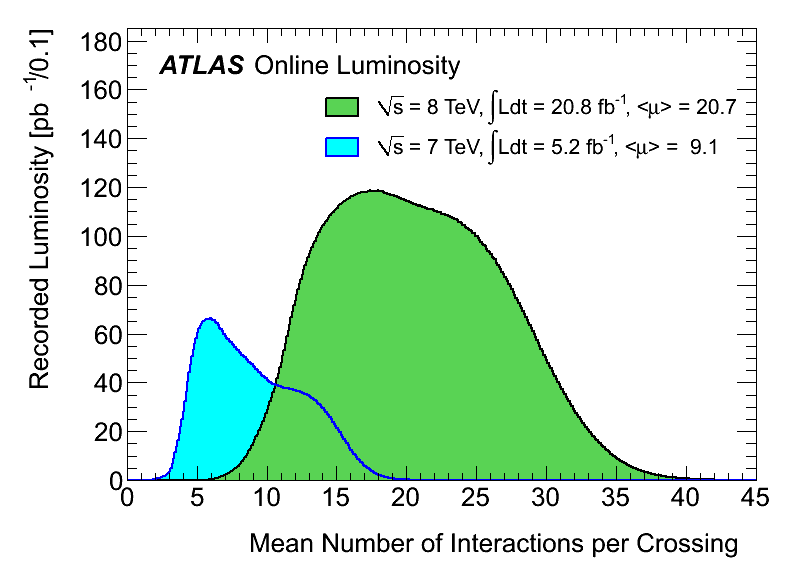
\includegraphics[width=.45\textwidth]{figures/lhc/pileup.png}
\caption{ (Left) The integrated luminosity as a function of time in 2012. The amount
delivered by the LHC is shown in green while the amount recorded by ATLAS
is overlayed in yellow. More than 93 \% of the integrated luminosity 
delivered by the LHC in 2012 was recorded by ATLAS.  
(Right) The distribution of pileup interactions recorded by ATLAS in 2011 and 2012.  }
\label{fig:lhc_lumi}
\end{figure}

%The LHC ran at a center-of-mass energy\footnote{Reduced from the design energy of 14 TeV.} from 2010 to 2011. 
In 2010 and 2011 the LHC operated at a center-of-mass energy of 7 TeV, while
in 2012 the LHC operated at a center-of-mass energy of 8 TeV\footnote{This
was reduced from the initial design energy of 14 TeV due to a quenching incident
in the superconducting dipole magnets in 2008 when running at full energy.}.
The peak luminosity and peak pileup versus time during these runs
are shown in the the top and bottom of \fig\ref{fig:lhc_conditions}, respectively.
This thesis focuses on the 8 TeV data collected in 2012.
This run had 
a bunch spacing of 50 ns, 1.6 to 1.7 $\times 10^{11}$ protons
per bunch, a beam radius of $18.8 \mu$m, and an average peak 
luminosity of $7.7 \times 10^{33}~\lumiunits$ \cite{Lamont:1709796}.
The luminosity lifetime, $\tau_L$, corresponding to \eqn\eqref{eq:lhc_lumi},
ranged from 7 hours to 14 hours during a single run \cite{Hostettler:2013qya}.
The total integrated luminosity in 2012 is shown 
on the left of \fig\ref{fig:lhc_lumi}.
The overall delivered integrated luminosity from the LHC
in 2012 was 23.3 \ifb, while that recorded was 21.7 \ifb. The 
amount of data recorded that is relevant for this thesis
and described in \sec\ref{sec:www} is slightly less at 20.3 \ifb.
The pileup conditions during 2012 were such that an average
of 20.7 collisions occurred per bunch crossing. The distribution
of the average interactions per crossing in 2011 and 2012 are shown on
the right of \fig\ref{fig:lhc_lumi}. The increase in the average pileup 
in 2012 is due to the increased peak luminosity.





%step through each section of the atlas detector
%could spend more time on the muon spectrometer (like the new EE A-side detectors)
%and more time on the muon trigger
%Clare put in the minimal detail (no more than 20 pages) while Jeremy had 50 pages
%I could maybe fit somewhere in between

%need to define Muon Spectrometer (MS)
%need to define Inner Detector (ID)
%Assumptions:
%Will describe trigger

\begin{figure}[ht!]
\centering
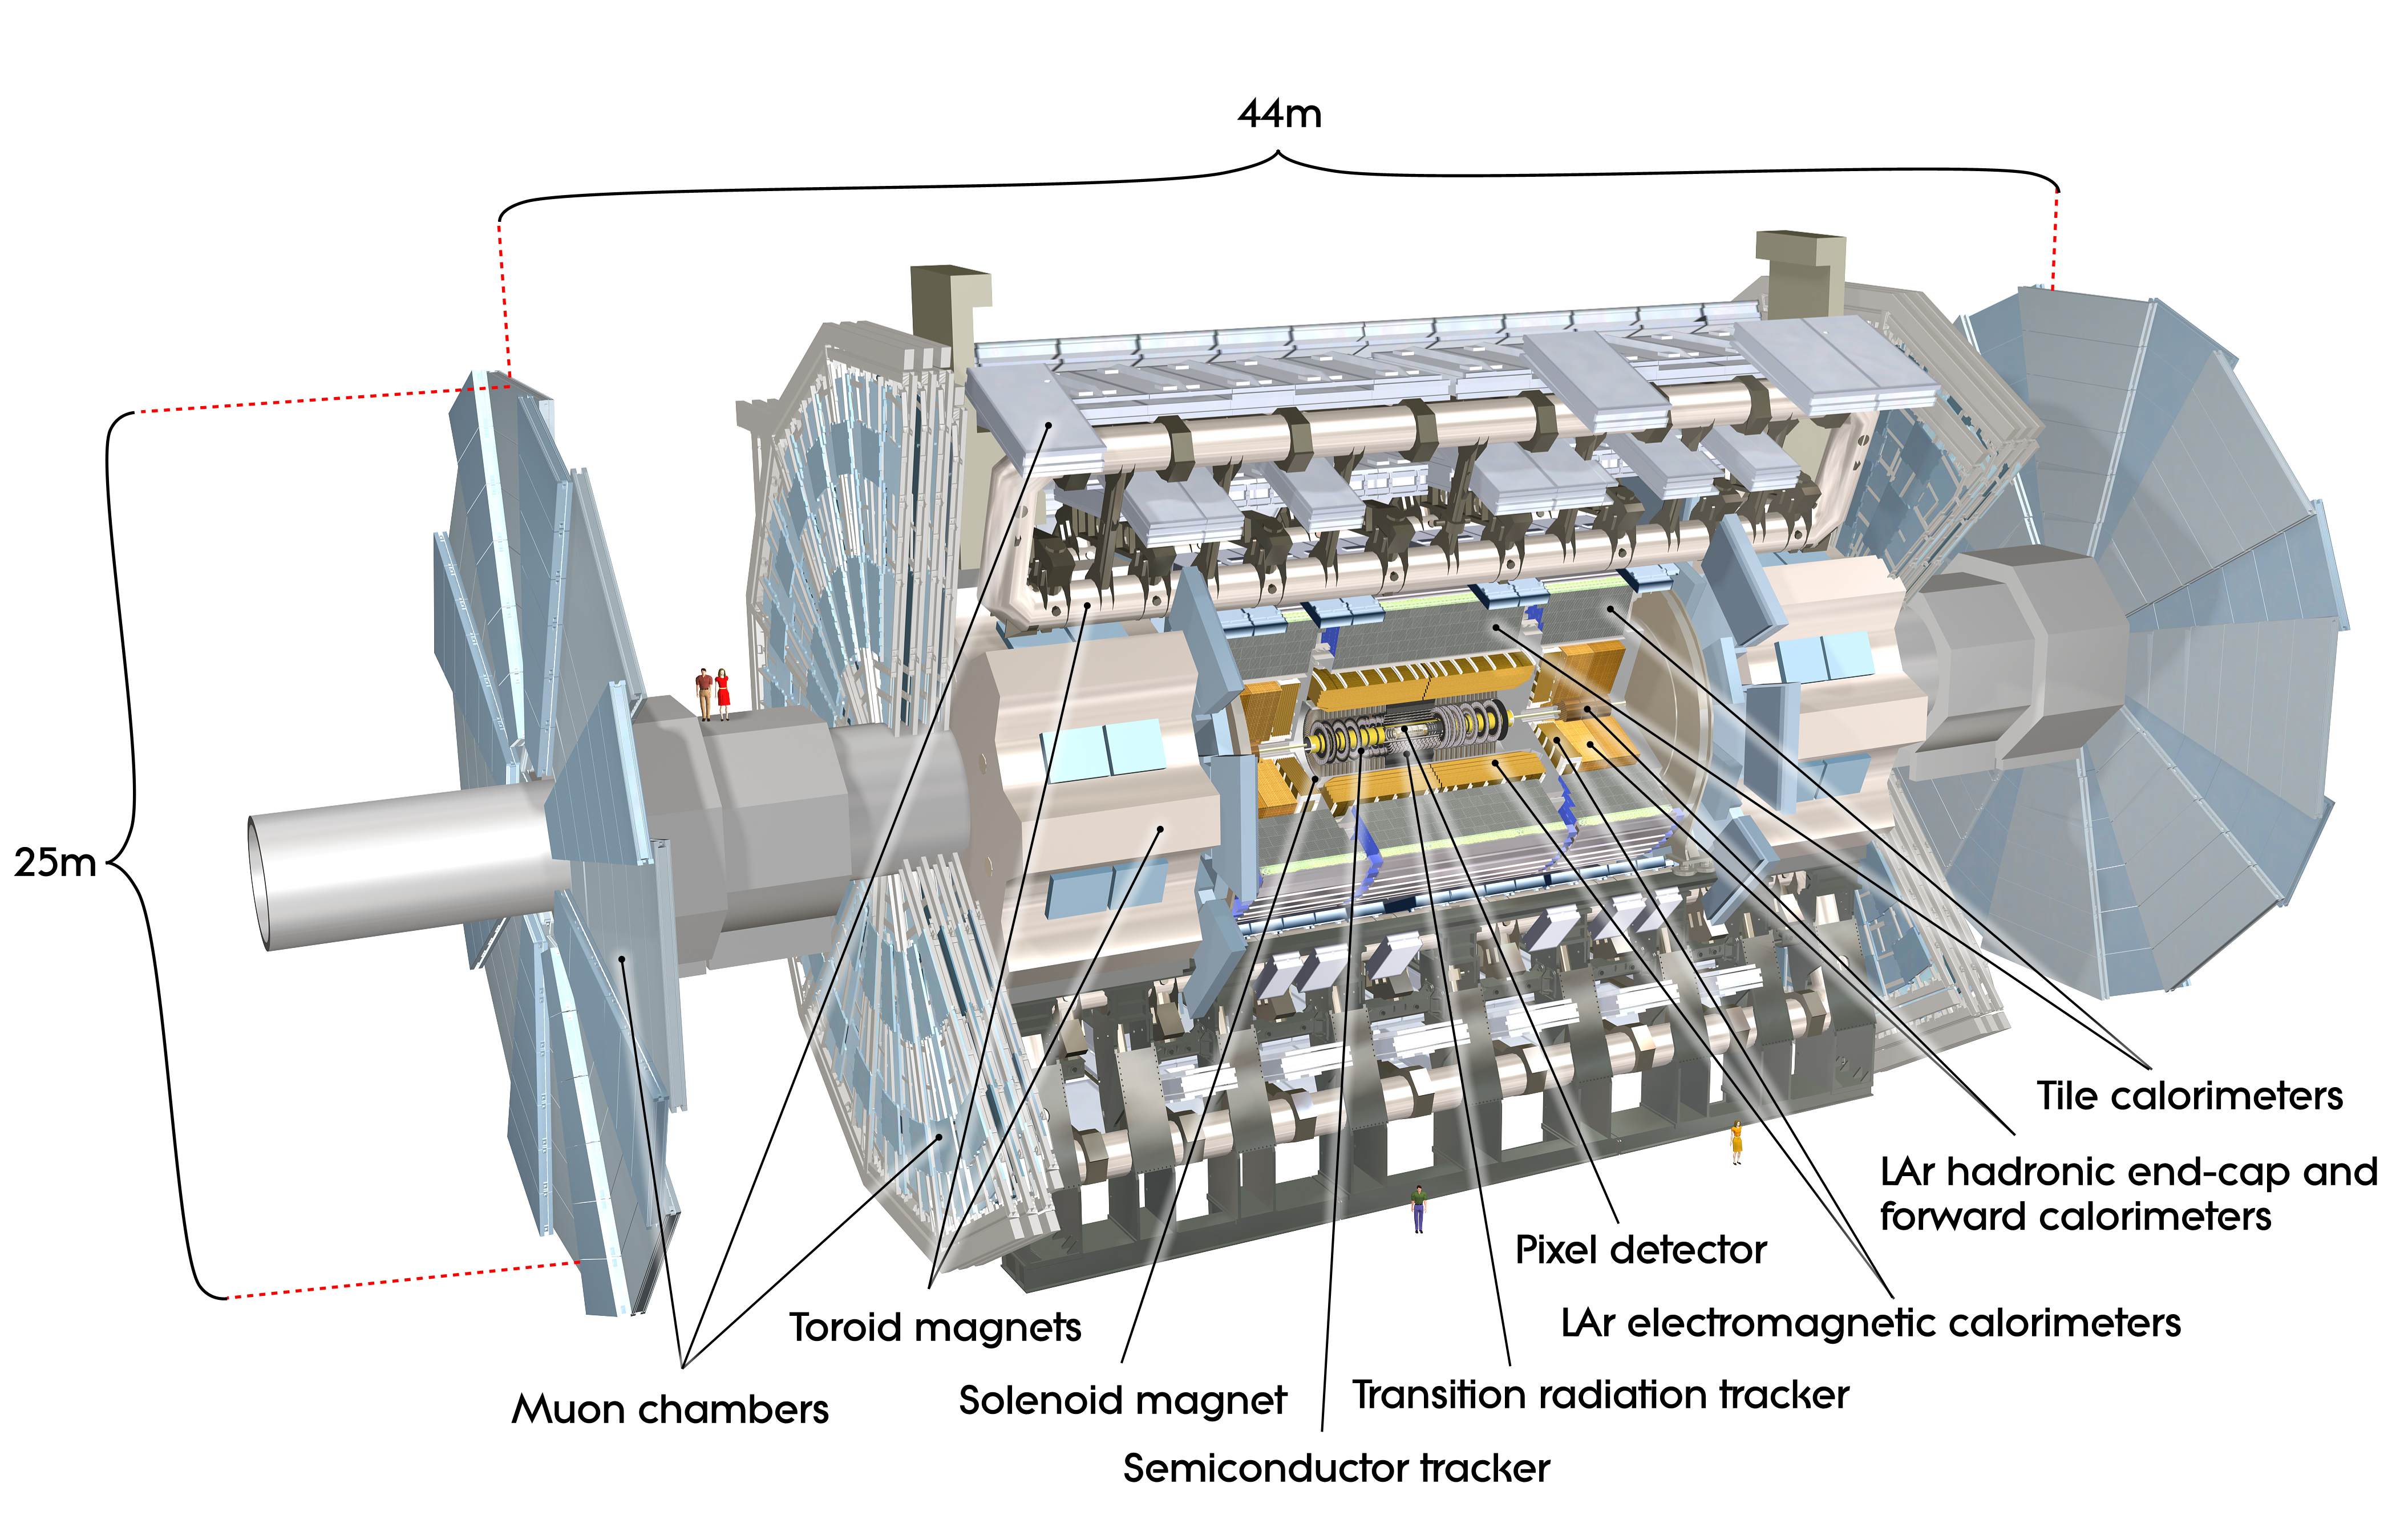
\includegraphics[width=.95\textwidth]{figures/atlas/detector.jpg}
\caption{A diagram of the ATLAS detector where the detector has
been artificially opened up to reveal the LHC beam line and the
various sub-detector components within. The sub-detector components
are labeled as such.}
\label{fig:atlas}
\end{figure}

%I need to define things here like eta, pt, deltaR, etc 
%I may need to talk about isolation here
The ATLAS detector~\cite{ATLAS} is designed to measure
the products of the particle collisions produced by the LHC.
In particular, the detector seeks to measure those stable 
(or meta-stable) particles whose decay lifetime is sufficiently
long enough to interact with the detector.  This includes
a variety of fundamental particles (like muons) as well as 
composite particles (like neutrons). The wide variety of 
particles to be measured requires the implementation
of several sub-detector systems that work in tandem 
to identify and measure their properties. 
A cylindrical geometry for the detector is chosen
which builds up around the beam line and surrounds
the collision point so that most of the collision
products will pass through it.
A diagram of the ATLAS detector can be seen in \fig\ref{fig:atlas}.
Its cylindrical shape is evident, with a diameter of 25 meters
and length of 44 meters. The detector is massive, weighing
in at roughly 7000 tonnes; but it is also highly granular, with
over 100 million detection elements that are arranged very precisely, 
in many cases on the order of tens of microns.
In the ``opened'' view of \fig\ref{fig:atlas}, the proton-proton
collisions from the LHC occur at the core of the detector
and the sub-detector components build up around this point.

The detectable products of the collision pass outward from the collision
point through the different components where their energy and momentum
are measured. The way in which the particles interact with the various
sub-detector systems helps to identify the types of 
particles produced.
This can be more clearly seen in the diagram of 
\fig\ref{fig:atlas_wedge}, which shows how the most typical
products of the LHC collisions interact with the different
components of the ATLAS detector.
Nearest the collision point is the inner detector (ID), designed to 
measure the paths of charged particles passing through using several
different subsystems. This 
is surrounded by a 2 Tesla solenoidal magnet.
The field from the magnet bends the trajectory of charged particles
in order to measure their momentum.
Beyond that is the calorimeter system
which measures the energy deposits of all particles passing 
through (except for neutrinos). The calorimeter system 
itself is divided up into components which fall into two main 
categories: the electromagnetic (ECAL)
and hadronic calorimeter (HCAL) systems.
The ECAL is situated in front of the HCAL and is designed
primarily to absorb and measure the energy and position of
electrons and photons. 
The HCAL is designed to do the same for
composite particles like protons and neutrons.
Surrounding the calorimeter system is the muon spectrometer (MS),
which is the largest component of the ATLAS detector and the one
that determines its size. It is designed to quickly identify and measure the 
trajectory of muons as they pass through
and leave the detector using precision 
and triggering components. The MS is also composed of 
three large superconducting air-core toroid magnets 
which allow for
a measurement of the muon momentum. The neutrinos 
pass through without interacting.

\begin{figure}[ht!]
\centering
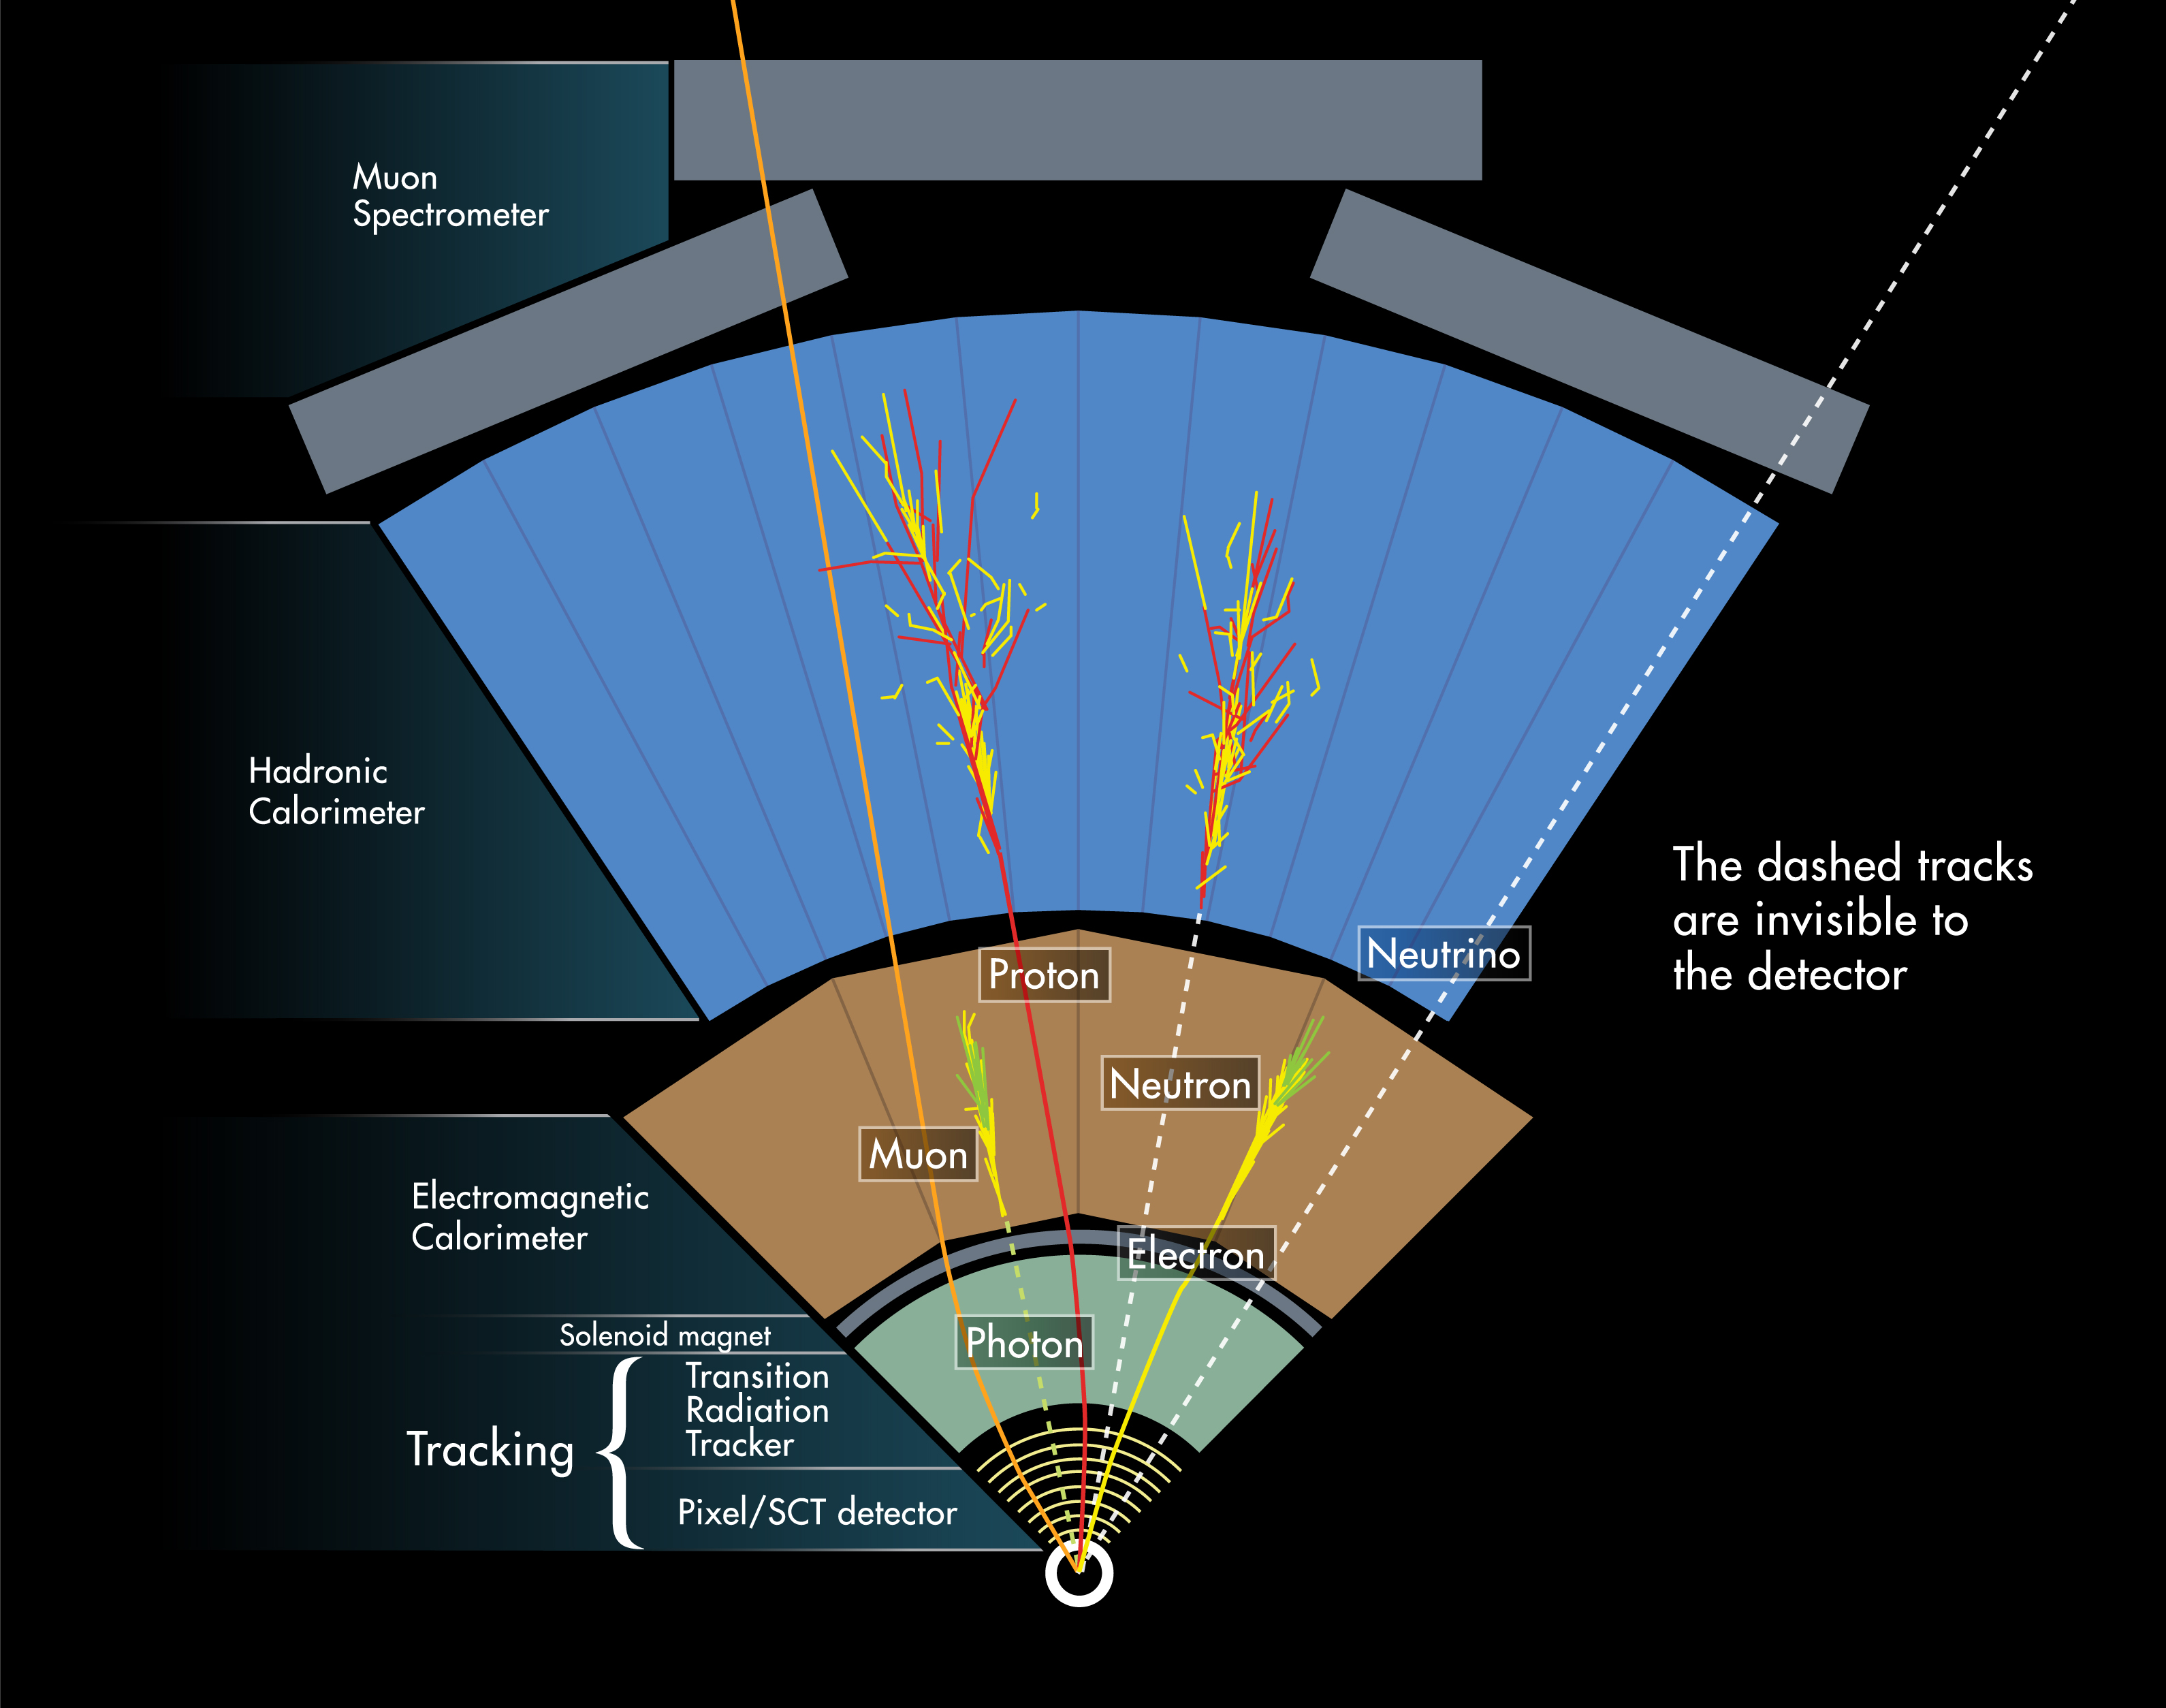
\includegraphics[width=.9\textwidth]{figures/atlas/wedge.jpg}
\caption{A diagram of one wedge of the ATLAS detector
as viewed from looking down the LHC beam line. 
The sub-detector components are shown along with the 
particles that typically come from the collision.
The paths of the particles are shown to indicate how each particle 
interacts with the detector.}
\label{fig:atlas_wedge}
\end{figure}

The geometry of the ATLAS detector is defined using a 
right-handed cylindrical coordinate system with the $x$-axis
pointing inwards towards the center of the LHC ring, the $y$-axis pointing
up, and the $z$-axis pointing along the beam-line, sometimes referred
to as the longitudinal or axial direction.
The $x-y$ plane, which is perpendicular to the beam-line,
is referred to as the transverse plane. In this plane, positions are  
defined using cylindrical coordinates with $r$ being the distance
from the beam-line and $\phi$ being the azimuthal angle.
The ATLAS detector has nearly uniform $2\pi$ 
coverage in $\phi$\footnote{While the ID and calorimeter systems are designed
to have minimal cracks in $\phi$, the
spatial extent of the MS makes this challenging due to service
and support structures. Thus, there are (sometimes large) 
cracks in the $\phi$ coverage in the MS.}.
For describing the direction of the particle with respect 
to the $z$-axis, a quantity called the rapidity, $y$,
can be related to the particle energy, $E$, and longitudinal momentum, $p_z$, 
by
\begin{equation}
y = \frac{1}{2} \ln \Bigg(\frac{E+p_z}{E-p_z} \Bigg),
\end{equation}
whose distribution is invariant under Lorentz boosts in the longitudinal direction.
This is a useful characteristic as the longitudinal momentum of the
partons within the proton are not known on an 
event-by-event basis, as discussed in \sec\ref{sec:pdf}.
At the LHC, most stable particles 
are produced with energies much larger than their mass.
In this limit, 
the rapidity can be simplified to a quantity called the pseudo-rapidity, $\eta$,
where
\begin{equation}
\eta = -\ln \tan (\theta/2) ,
\label{eq:pseudorapidity}
\end{equation}
which is only a function of the polar angle, $\theta$, 
the direction of the particle with respect to the positive $z$-axis.
The distribution of rapidity for the inclusive cross-section
at the LHC falls mostly within the ATLAS ID and MS detector volumes 
of $|\eta| < 2.5$ and $|\eta| < 2.7$, respectively, 
though the calorimeter system is extended out to $|\eta| < 4.9$
in order to ensure good coverage.

The transverse momentum of charged tracks can be determined by measuring how they 
bend in a magnetic field. The deviation of the trajectory
from a straight line path is referred to as the 
sagitta\footnote{Technically, the sagitta, $s$, is defined in terms
of an arc as the distance from the center of the arc to the center of its
base. It can be related to the radius of the arc, $r$, and half the length
of the line connecting the two ends of the arc, $l$, by 
$s=r-\sqrt{r^2-l^2}$.}, $s$. The sagitta is proportional to the magnetic
field strength and inversely proportional to the magnitude
of the particle's momentum in the transverse plane, known
as the transverse momentum or \pt.
Thus, a straight-line trajectory resembles an infinite-momentum charged
particle (or a neutral particle of any momentum), while
a bent trajectory corresponds to a charged particle with a finite momentum.
As a result, the transverse momentum resolution, $\Delta p_T$, is related to the 
precision on the measurement of the sagitta, $\Delta s$ by
\begin{equation}
\frac{\Delta p_T }{p_T} = \frac{\Delta s}{s} .
\label{eq:sagitta}
\end{equation}
This has the effect that the relative uncertainty on the momentum
measurement grows linearly as a function of the momentum.


The total momentum of the proton-proton collision in the transverse
plane is nearly zero. Since the detector has nearly full azimuthal coverage 
in the transverse plane, we can test this constraint by measuring
the total transverse momentum from the particles measured in the detector
such that
\begin{equation}
\Bigg| \sum_{i\in\textrm{All Particles}} \overrightarrow{p_{\textrm{T},i}} \Bigg| = 0,
\end{equation}
where the transverse momentum is added vectorialy and then
the magnitude is taken.
After adding up the $\pt$ of all of the particles to obtain
the total transverse momentum, 
any imbalance with respect to this constraint
is referred to as the
missing transverse energy
and is attributed to the 
neutrinos produced in the collision.
Thus, it is a vector defined as
\begin{equation}
\vecmet = -\Bigg( \sum_{i\in\textrm{All Particles}} \overrightarrow{p_{\textrm{T},i}} \Bigg),
\label{eq:met}
\end{equation}
though usually we are just 
interested in its magnitude, $\met = |\vecmet|$.
There is no such constraint on the longitudinal momentum of the partons
on an event-by-event basis
as discussed in \sec\ref{sec:pdf}.
This is the case
even though the momentum of the protons along the $z$-direction
is, in fact, known.
Thus, there is no direct way of determining with certainty the 
momentum of the neutrinos in the $z$-direction.



\section{Inner Detector}
\label{sec:atlas_id}

\begin{figure}[htb]
\centering
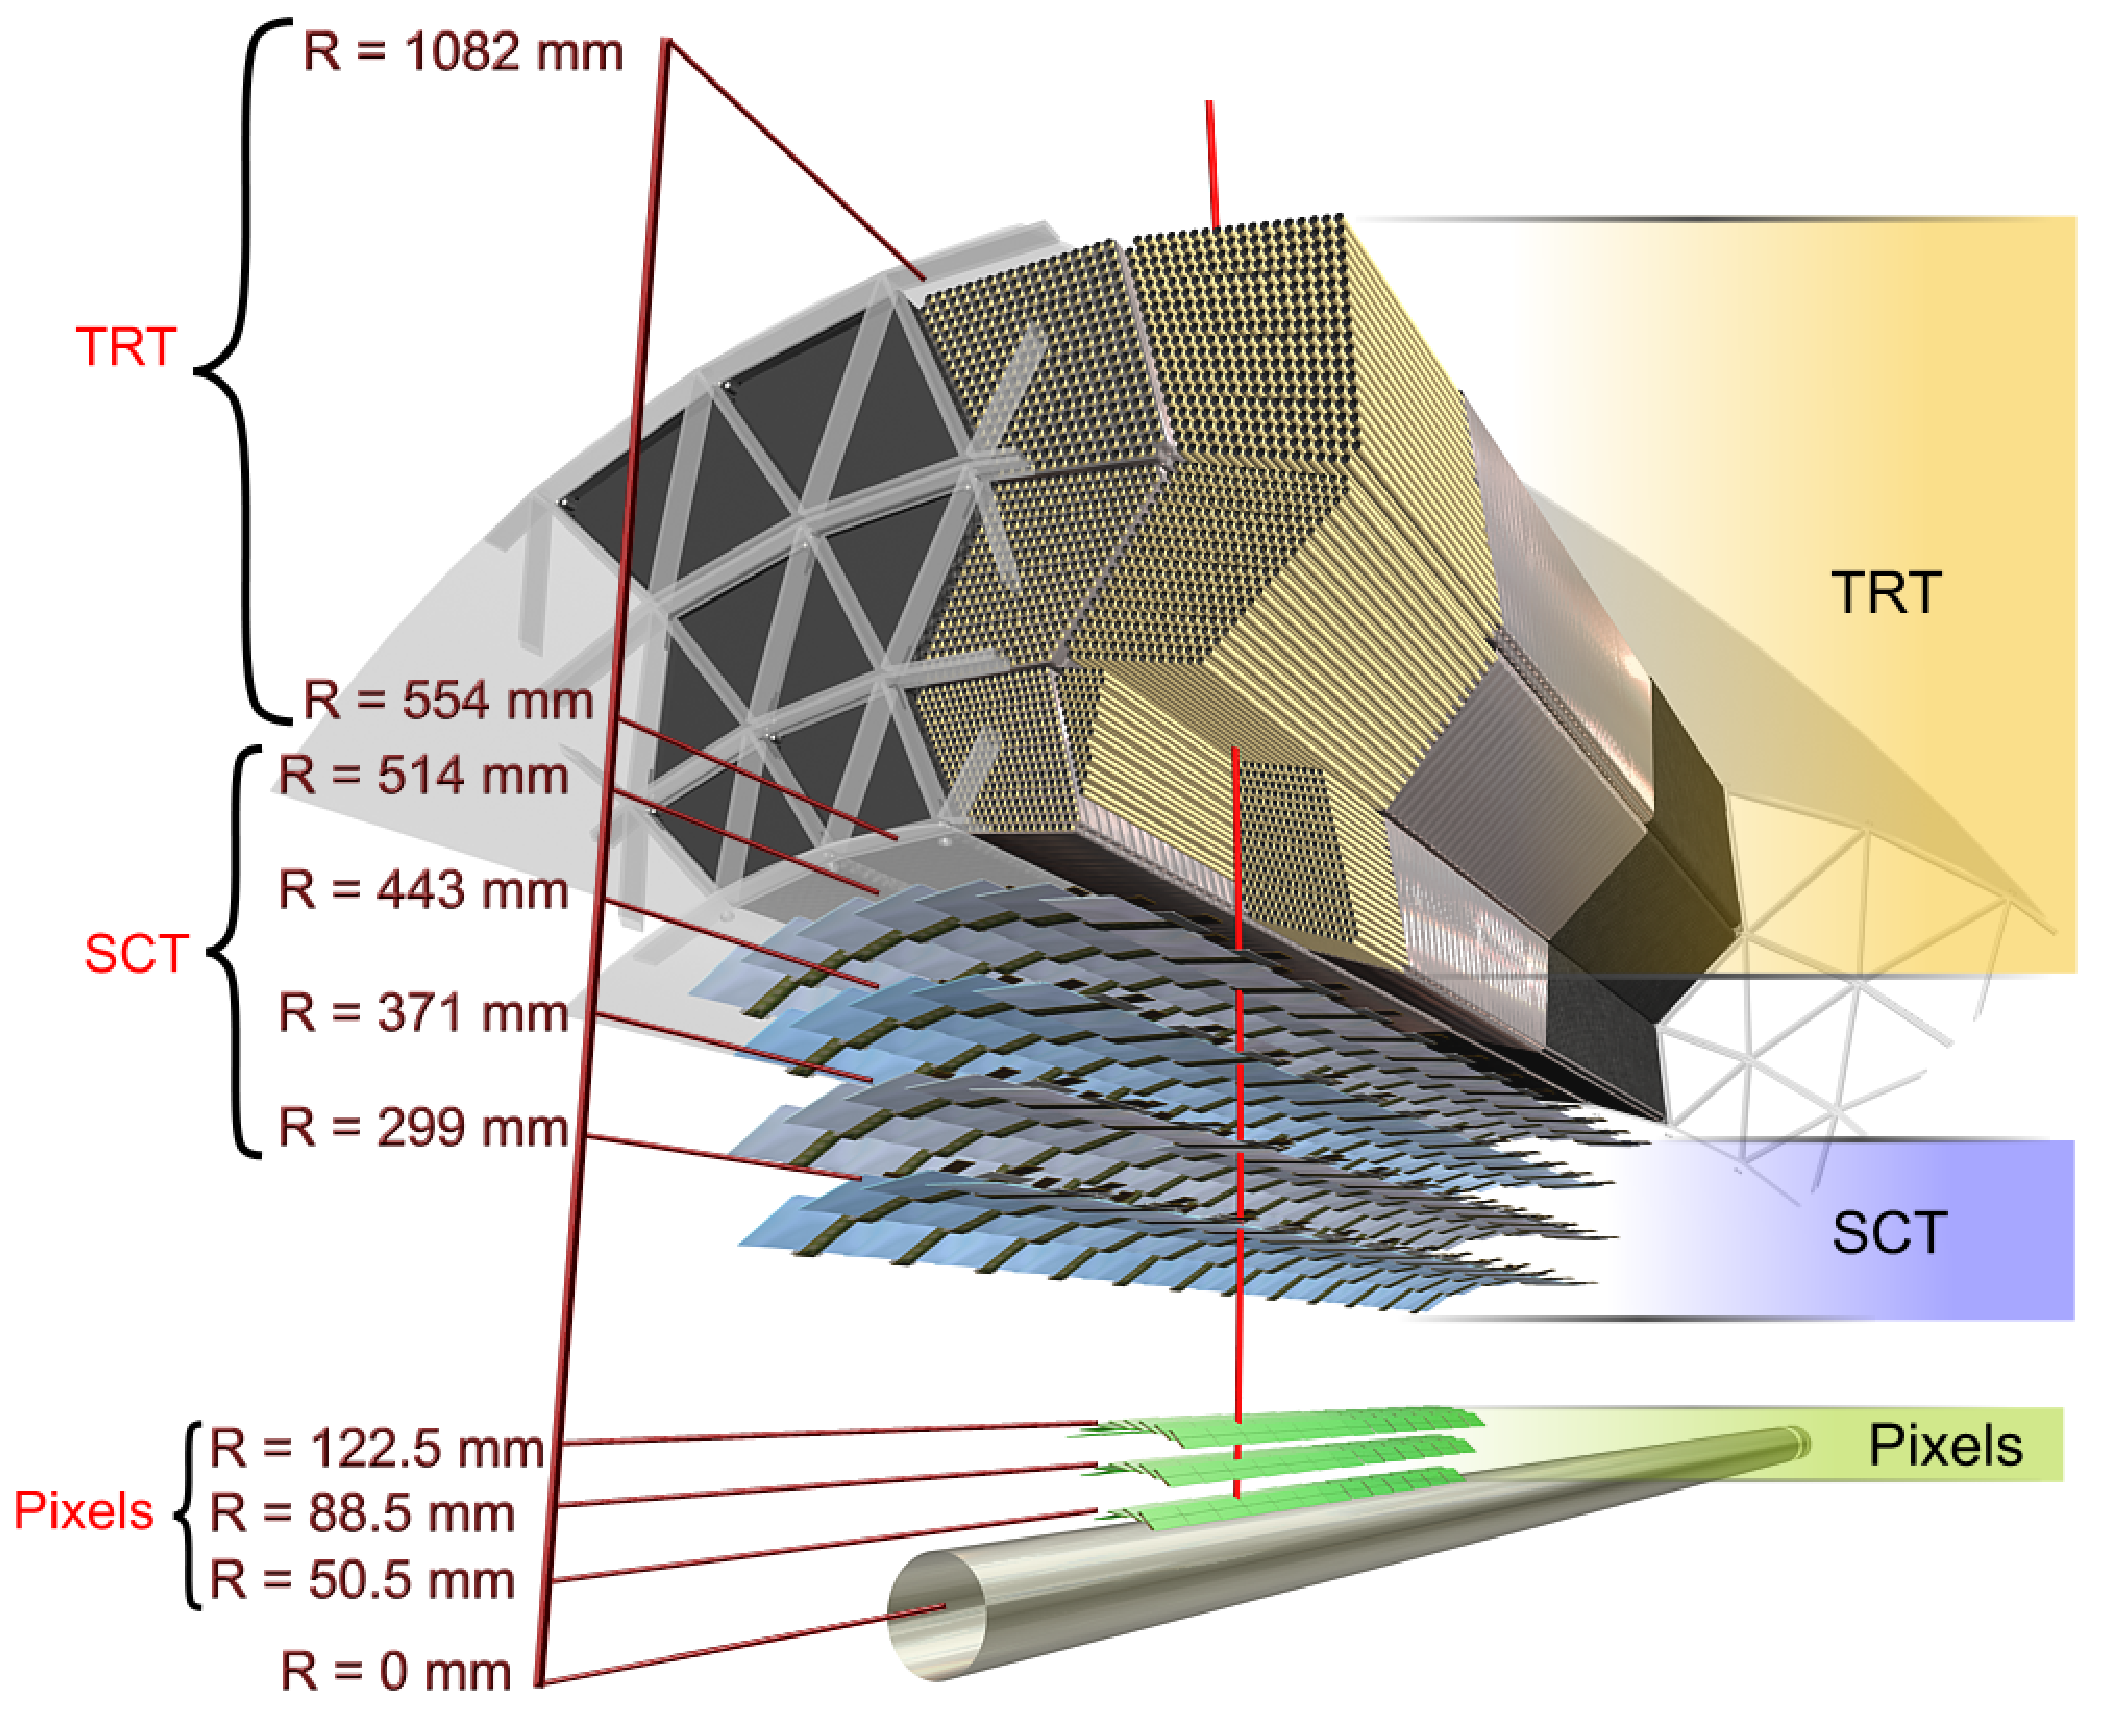
\includegraphics[width=0.8\textwidth]{figures/atlas/id_barrel.eps}
\caption{Diagram of the ATLAS Inner Detector (ID) showing 
a wedge of the barrel system.  The three detector systems
are clearly labeled. The LHC beam pipe is axial to the system
and is shown at the bottom of the diagram.}
\label{fig:atlas_id_barrel}
\end{figure}

\begin{figure}[htb]
\centering
\includegraphics[width=0.95\textwidth]{figures/atlas/id_endcap.eps}
\caption{Diagram of the ATLAS Inner Detector (ID) showing 
a wedge of the end-cap system as well as a part of the SCT and Pixel
barrel systems.  The detector systems
are clearly labeled.  The LHC beam pipe is axial to the system
but is not shown. Trajectories of two charged tracks 
with a $\pt=10\GeV$ are shown along $\eta=1.4$ and $\eta=2.2$ as
indicated by the solid bright red lines.}
\label{fig:atlas_id_endcap}
\end{figure}

The inner detector (ID) is the 
detector system that is closest to the beam pipe and thus the
first system that the products of the LHC collisions encounter
on their way from the collision point. Its primary role is 
to measure the trajectory and momentum of charged particles
via ionization as they pass through the detector.
It must be capable of measuring these tracks with high precision
in order to obtain precise momentum measurements. It must
also be able
to accurately extrapolate the tracks back to the collision point.
This allows one 
to obtain primary and secondary interaction vertices with adequate
resolution for overcoming pileup 
conditions (see \sec\ref{sec:lhc_collider_physics}). In addition,
since the system is so close to the LHC beam line, it
must be able to handle high particle fluxes. This requires that
the ID must have a very high granularity and fast electronics
readouts such that the occupancy of the
detector is small enough to distinguish between individual tracks. 
The detector materials and electronics must also be sufficiently radiation
hard that they can withstand years of LHC 
exposure time\footnote{The layer of the pixel detector that is closest
the beam line is subjected to so much radiation that it is expected to be replaced
every three years.  Meanwhile, the radiation exposure of the other ID
components drops off rapidly (already by a factor of 6 for the third
pixel layer and by over a factor of 200 for the outer TRT) and is 
expected to survive for the planned lifetime of the detector.}.
These tough requirements push the limits of available technology and thus
make the ID the most sophisticated detector system in ATLAS.



\begin{figure}[htb]
\centering
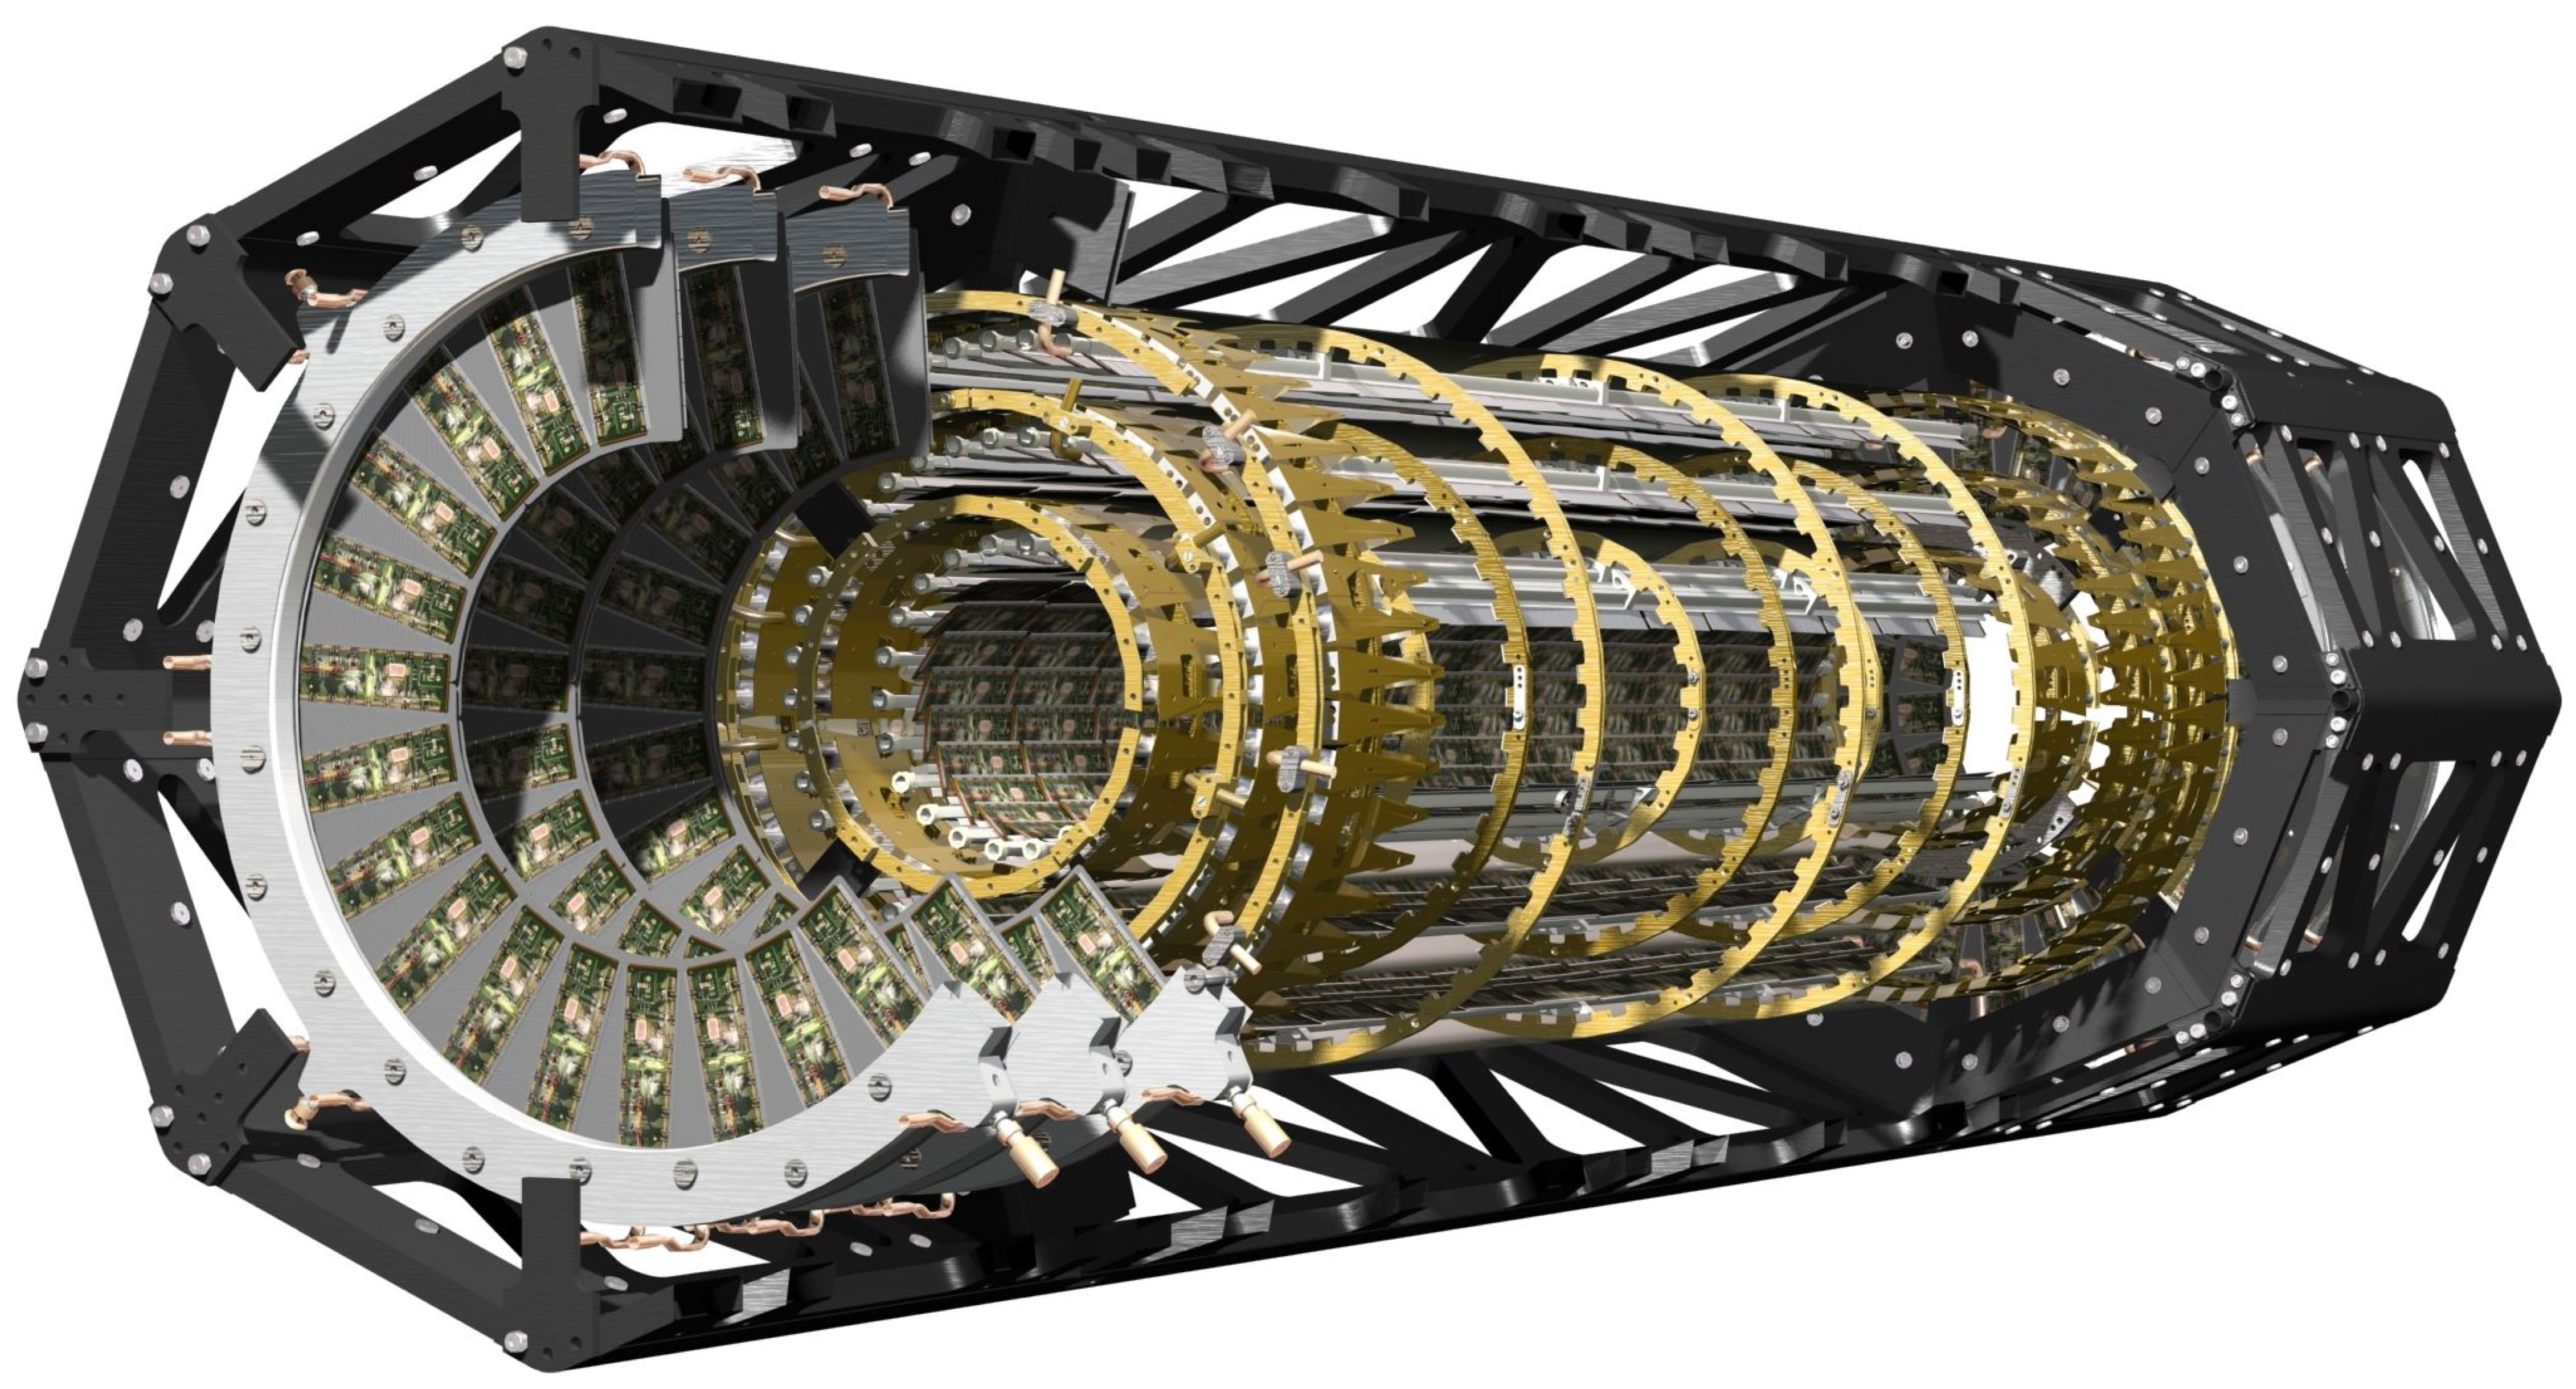
\includegraphics[width=0.7\textwidth]{figures/atlas/pixel.eps}
\caption{A cut-out diagram of the ATLAS pixel detector showing 
the arrangement of the pixel modules (green) in three layers of the barrel
and three layers of one end-cap system. Some of the support structure is
also shown.}
\label{fig:atlas_pixel}
\end{figure}

There are three different detector subsystems within the ID, together
immersed in a uniform 2 Tesla axial magnetic field: the pixel detector,
the silicon microstrip tracker (SCT), and the transition radiation
tracker (TRT). These three detector systems can be seen 
in the barrel in \fig\ref{fig:atlas_id_barrel} and from an alternate
view also showing one of the end-caps in \fig\ref{fig:atlas_id_endcap}. 
The pixel detector
is composed of more than seventeen hundred thin doped silicon sensors with 
dimension $19~\textrm{mm} \times 64~\textrm{mm}$. Each sensor has more than forty-six
thousand readout elements (with a 
nominal size of $50 ~\mu\textrm{m} \times 400~\mu\textrm{m}$),
corresponding to the ``pixels'' which give the detector its name. 
A charged particle passing through an individual pixel produces a signal
which identifies its location. The combination of 
several layers can thus be used to form the trajectory of the particle. %sagitta
Each sensor is attached to a single readout electronic board, which comprises
one module.
The modules are arranged into three cylindrical barrel layers (at 
$r = $ 51 mm, 89 mm, and 120 mm)  and 
two end-caps each with three disk-shaped layers (at $|z| = $ 500 mm, 580 mm, 
and 650 mm) such that there is uniform
azimuthal coverage. A cut-out diagram of the pixel detector 
structure with modules in place in both the barrel and end-caps is shown 
in \fig\ref{fig:atlas_pixel}. The barrel covers roughly 
$|\eta|<1.7$ and the two end-caps roughly $1.7<|\eta|<2.5$.
The 
spatial resolution of the pixel detector is around $10~\mu\textrm{m}$ in 
the $R-\phi$ plane and $115 ~\mu\textrm{m}$ 
orthogonal to this plane \cite{ATLAS-CONF-2014-047}.



The SCT uses almost sixteen thousand thin silicon strip sensors, though not of the 
same type as in the pixel detector. 
A barrel silicon strip sensor 
has dimension $6.36~\textrm{cm} \times 6.40~\textrm{cm}$
with 768 readout strips running along the longer dimension. The barrel
strips are placed in four concentric cylindrical layers, uniformly in azimuth
(at $r = $300 mm, 370 mm, 440 mm, and 510 mm).
They are aligned axially with a strip pitch of 
80 $\mu$m, and covering roughly
$|\eta|<1.4$, as can be seen in \fig\ref{fig:atlas_id_barrel}.
In each of the two end-caps the sensors are made to form nine
disks spaced apart along the axial 
direction (at $|z| = $0.85 m, 0.93 m, 1.1 m, 1.3 m, 1.4 m, 
1.8 m, 2.1 m, 2.5 m, and 2.7 m) covering roughly $1.4 < |\eta|<2.5$, 
as seen in \fig\ref{fig:atlas_id_endcap}. The strips are similar
to those in the barrel except that they are tapered along the strip direction.
The sensors are then oriented such that the taper expands radially outward
with a strip pitch ranging from 60 $\mu$m to 90 $\mu$m as $|z|$ increases.
The spatial resolution is about $17~\mu\textrm{m}$
in the $R-\phi$ plane \cite{ATLAS-CONF-2014-047}. 
Due to the length of the strips, the precision is considerably
worse in the axial direction for the barrel and the radial direction for 
the end-caps, with a precision of roughly $580~\mu\textrm{m}$.


The TRT uses a fundamentally different technology 
than the pixel and SCT.
Drift tubes are used of 4~mm in diameter 
which are filled with a Xenon-based gas mixture
and with an anode wire running through the center.
The tubes can be placed in close
proximity such that many measurements, around 36,
can be made on a single charged track. An important feature
of the TRT is its ability to identify electrons using transition radiation.
The tubes are surrounded in polypropylene material which  induce
transition radiation from incident highly relativistic charged particles.
The transition radiation photons are absorbed by the Xenon in the gas
which amplifies the signal. The effect is strongest for electrons, 
which allows for excellent discrimination between electrons
and other charged particles, like pions.
The barrel TRT runs from roughly $|\eta|<0.7$ and
is constructed from 144 cm long straws aligned
axially. Over fifty-two thousand straws are interleaved
with polypropylene fibers to form 73 layers of straws 
spaced roughly 7 mm apart and surrounding the beam-pipe with
a cylindrical symmetry and uniform coverage in azimuth,
as seen in \fig\ref{fig:atlas_id_barrel}.
In each of the two end-caps, two wheels are formed from over seventy-three
thousand straw tubes, 37 cm in length, 
oriented and distributed uniformly in azimuth. 
The inner wheel is formed from twelve layers and the outer wheel from eight
layers of straws spaced 8 mm and 15 mm apart, respectively,  
with 768 straws per layer, seen in \fig\ref{fig:atlas_id_endcap}.
The end-caps cover roughly $0.7<|\eta|<2.2$.
An individual straw has a precision of about $130~\mu\textrm{m}$ along
its diameter \cite{ATLAS-CONF-2014-047}.




%efficiency of electron identification?  large number of readouts?  occupancy??  noise??  sagitta???  explain how the b-field is used?  eta coverage?  materials?  electronics?  more figures?  
\section{Calorimeters }
\begin{figure}[ht]
\centering
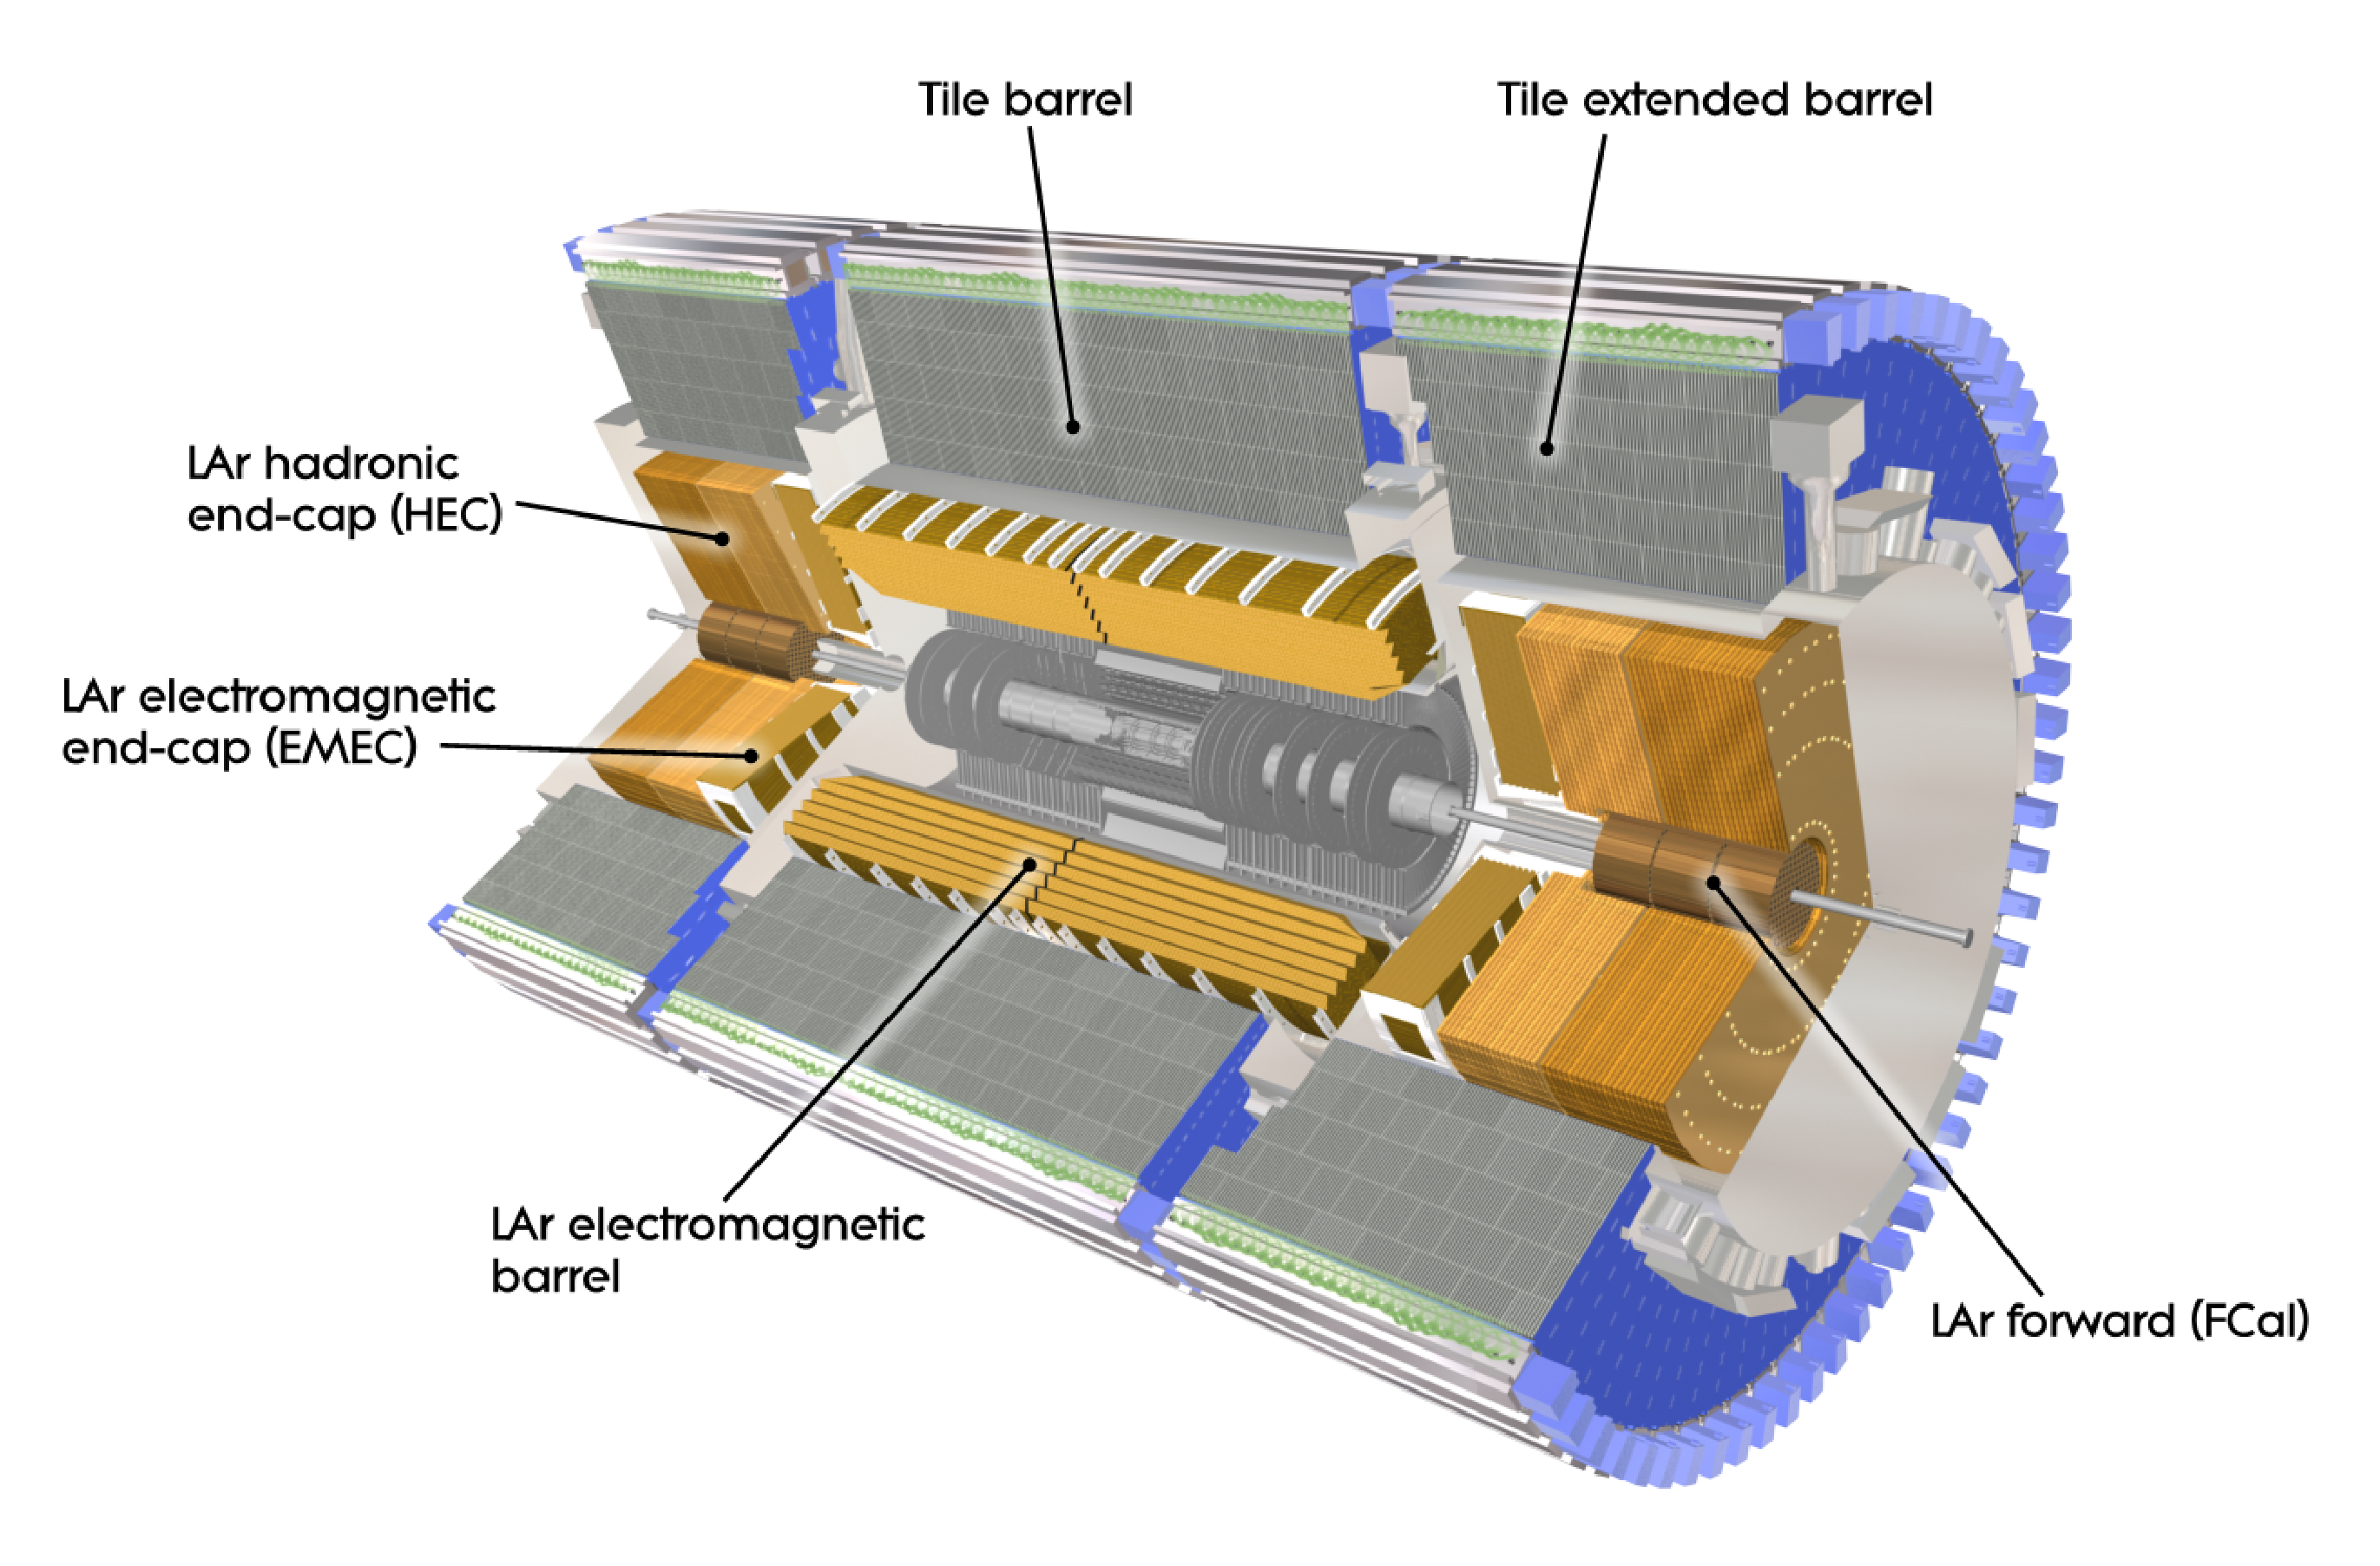
\includegraphics[width=0.9\textwidth]{figures/atlas/calorimeter.eps}
\caption{Diagram of ATLAS calorimeter system with cut-out portion
to allow a view of the nested sub-components.}
\label{fig:atlas_calorimeter}
\end{figure}


\begin{figure}[ht]
\centering
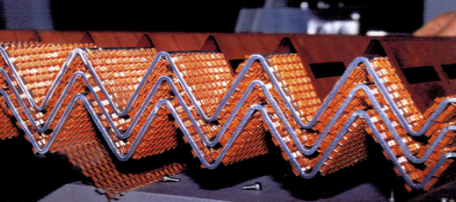
\includegraphics[width=.7\textwidth]{figures/atlas/emcal_accordion.png}
\caption{Photo of three ECAL sampling layers
showing its accordion-like structure. In the picture, 
the horizontal directions corresponds to 
the radial direction when the detector is in position, which is
the direction the LHC products would follow.}
\label{fig:atlas_emcal_accordion}
\end{figure}

\begin{figure}[ht]
\centering
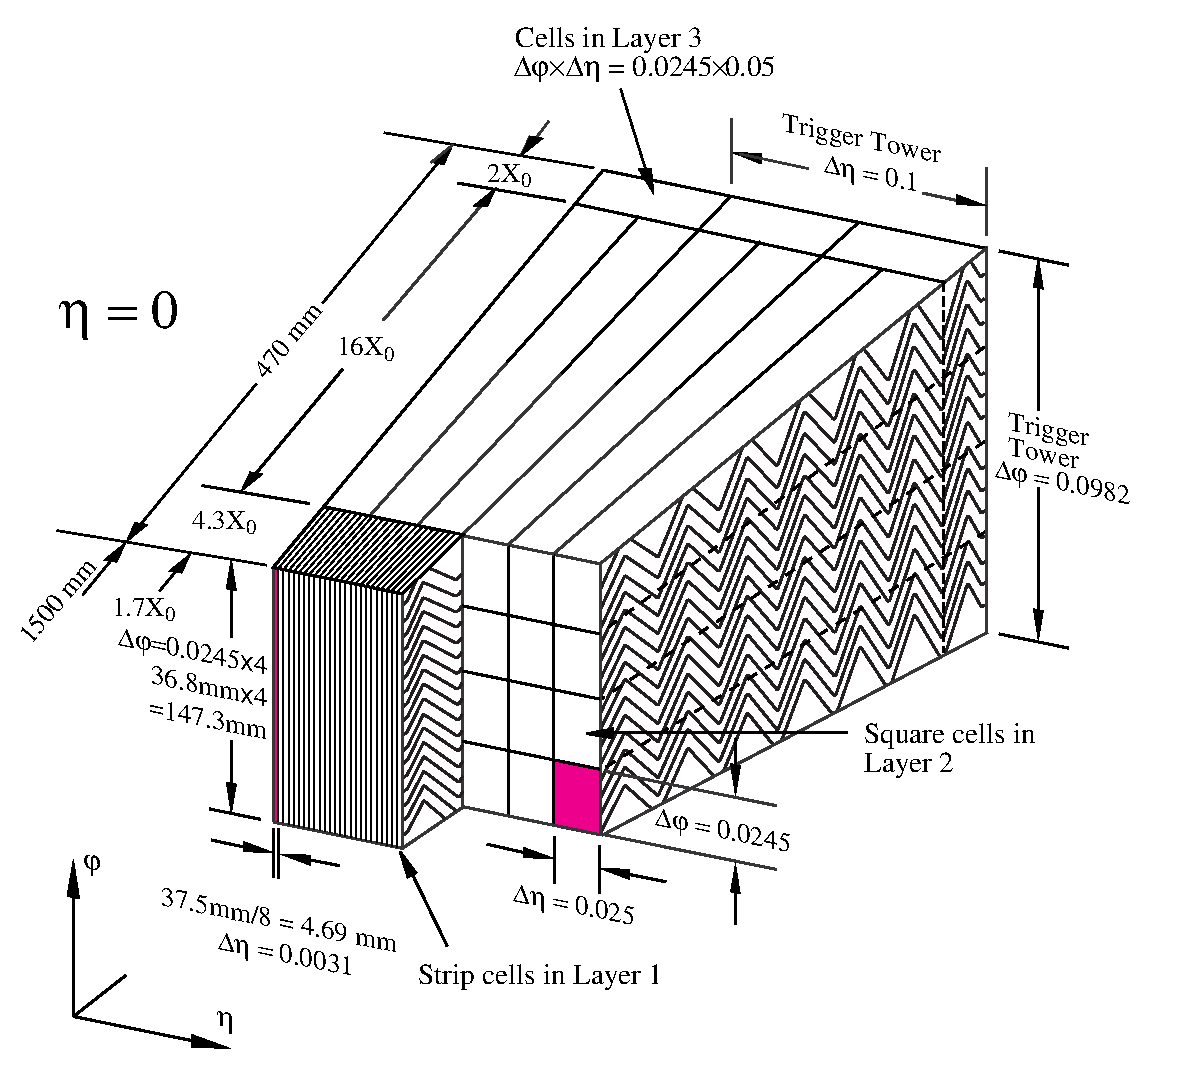
\includegraphics[width=.8\textwidth]{figures/atlas/emcal_barrel_module.eps}
\caption{ A diagram of one ECAL barrel module 
covering $22.5^{\circ}$ in azimuth. When inside the detector,
it is oriented as indicated by the axes.}
\label{fig:atlas_emcal_module}
\end{figure}

The ATLAS calorimeter is designed to measure the energy
deposits of the products of the LHC collisions which pass through
it except for the neutrinos.  A diagram of the 
calorimeter system can be seen in \fig\ref{fig:atlas_calorimeter}.
The calorimeter system is split into four main systems:
the electromagnetic calorimeter (ECAL), the 
tile hadronic calorimeter (HCAL), the hadronic 
end-cap calorimeter (HEC), 
and the Forward Calorimeter (FCAL).
Each system is optimized to measure either electromagnetic
or hadronic calorimeter deposits, though there is no
way to make this exclusive; in general,
electromagnetic and hadronic particles will interact with both.
The amount of energy incident particles will lose due to electromagnetic
interactions in a material can be quantified by measuring the material thickness
in units of radiation length, \xzero. Similarly, the amount of energy loss
due to hadronic interactions can be quantified by measuring the material
thickness in units of interaction length, $\lambda$.
Those calorimeter systems optimized for measuring electromagnetic 
energy deposits generally have high radiation length and low interaction
length. They are then placed in front of the calorimeter systems
optimized for measuring hadronic energy deposits which have high
interaction lengths, though
the radiation length is usually also large.
%material plot


The ECAL is a sampling calorimeter that uses lead as the sampling
medium and liquid Argon (LAr) as
the active medium from which the charge of the electromagnetic
shower produced by incident particles on the sampling medium
can be collected.  LAr is used as the active medium 
because of its radiation hardness and its linear response.
%as evidenced in \fig\ref{fig:atlas_emcal_response}.
The lead sampling medium alternates with the active LAr medium
using lead sheets 1 to 2~mm thick with an approximately 4~mm wide
LAr gap between each sheet and electrodes placed in the middle of
the gaps.
The lead sheets are constructed using a unique ``accordion''-like structure,
as seen in \fig\ref{fig:atlas_emcal_accordion}. 
This is to provide a uniform resolution with no gaps
in the azimuthal direction.
The ECAL itself can be split up into a barrel region ranging
from $0<|\eta|<1.3$ and two end-cap regions ranging from 
$1.5 < |\eta| < 3.2$.
The thickness of the barrel region 
ranges from $22~\xzero$ to $30~\xzero$
for $|\eta|<0.8$ and from $24~\xzero$ to $33~\xzero$ for
$0.8 < |\eta| < 1.3$.
The barrel region is divided into individual modules
which together surround the beam-line
in a cylindrical shape.  A diagram of one such module
can be seen in \fig\ref{fig:atlas_emcal_module}.
From this one can see that each module is segmented in $\eta$
and $\phi$, as well as into three layers in depth.
Segmentation is applied to obtain pointing information, 
which aids in the identification and measurement of electromagnetic
objects in conjunction with measurements from the ID,
and also shape information about the shower, which is useful
for particle identification\footnote{For instance,
the fine segmentation can be used to resolve the two
separate showers separated by a small opening angle in 
$\pi^0\to\gamma\gamma$ decay.}.
The very fine segmentation in $\eta$ of the first layer
in depth is important for precision tracking and shape measurements.
The second layer has a larger depth and thus collects most of the energy.
There are two identical end-cap regions, one on each side of the 
collision point. Each end-cap region consists of two wheels: the 
outer wheel from $1.4756 < |\eta| < 2.5$, with a thickness ranging from
$24~\xzero$ to $38~\xzero$, and 
the inner wheel from $2.5 < |\eta| < 3.2$, with a thickness ranging from
$26~\xzero$ to $36~\xzero$.
The regions from $1.5 < |\eta|<2.5$ in the inner and outer wheels both
have three layers, with the first being a finely segmented precision
layer similar to the barrel regions. Outside this region there 
are only two layers with a coarser segmentation.
The ECAL also consists of a pre-sampler detector with a single layer of LAr in 
front of the full barrel ECAL and in front of the end-cap ECAL 
from $1.5 < |\eta| < 1.8$. This aids in the measurement of the energy deposits
prior to reaching the ECAL and allows 
for a better understanding of the energy deposited
in the transition region between the barrel and end-caps.


\begin{figure}[ht]
\centering
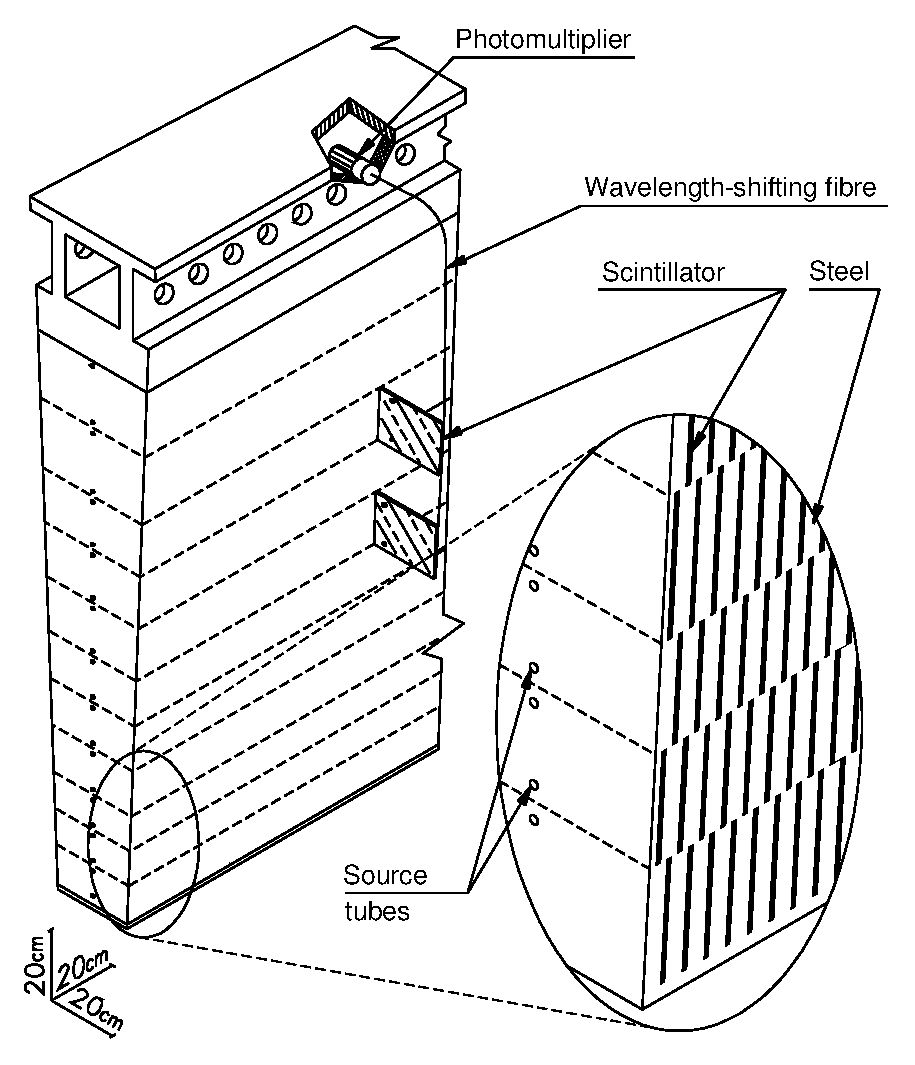
\includegraphics[width=.6\textwidth]{figures/atlas/hcal_module.eps}
\caption{ A diagram of one tile HCAL module 
covering $5.625^{\circ}$ in azimuth. The radial direction when 
positioned in the detector corresponds to the vertical direction in the
image.}
\label{fig:atlas_hcal_module}
\end{figure}


The tile HCAL is a steel sampling calorimeter with scintillating tiles used as the 
active material.
Steel is chosen as the sampling material since it gives a good
depth in interaction lengths  with a maximum depth
of $7.4~\lambda$, while also having a low cost.
It is split into a central barrel and two extended barrels 
which together cover a 
region from $|\eta|< 1.7$, as can be seen in \fig\ref{fig:atlas_calorimeter}.
As in the ECAL barrel, the tile HCAL is divided into individual modules
that surround the collision point in azimuth. A diagram of one such
module is shown in \fig\ref{fig:atlas_hcal_module}.
The scintillating tiles alternate periodically with the self-supporting
steel body and are oriented radially. 
The scintillation
light is routed through wavelength-shifting fibers and collected
at photo-multiplier tubes placed at the back of the module.
This configuration allows for a near uniform coverage in azimuth.  
In the crack region from $1.2 < |\eta| < 1.6$ between the central barrel 
and extended barrels, special modules are placed to recover and correct
for energy losses in this region.

\begin{figure}[tb] 
\centering
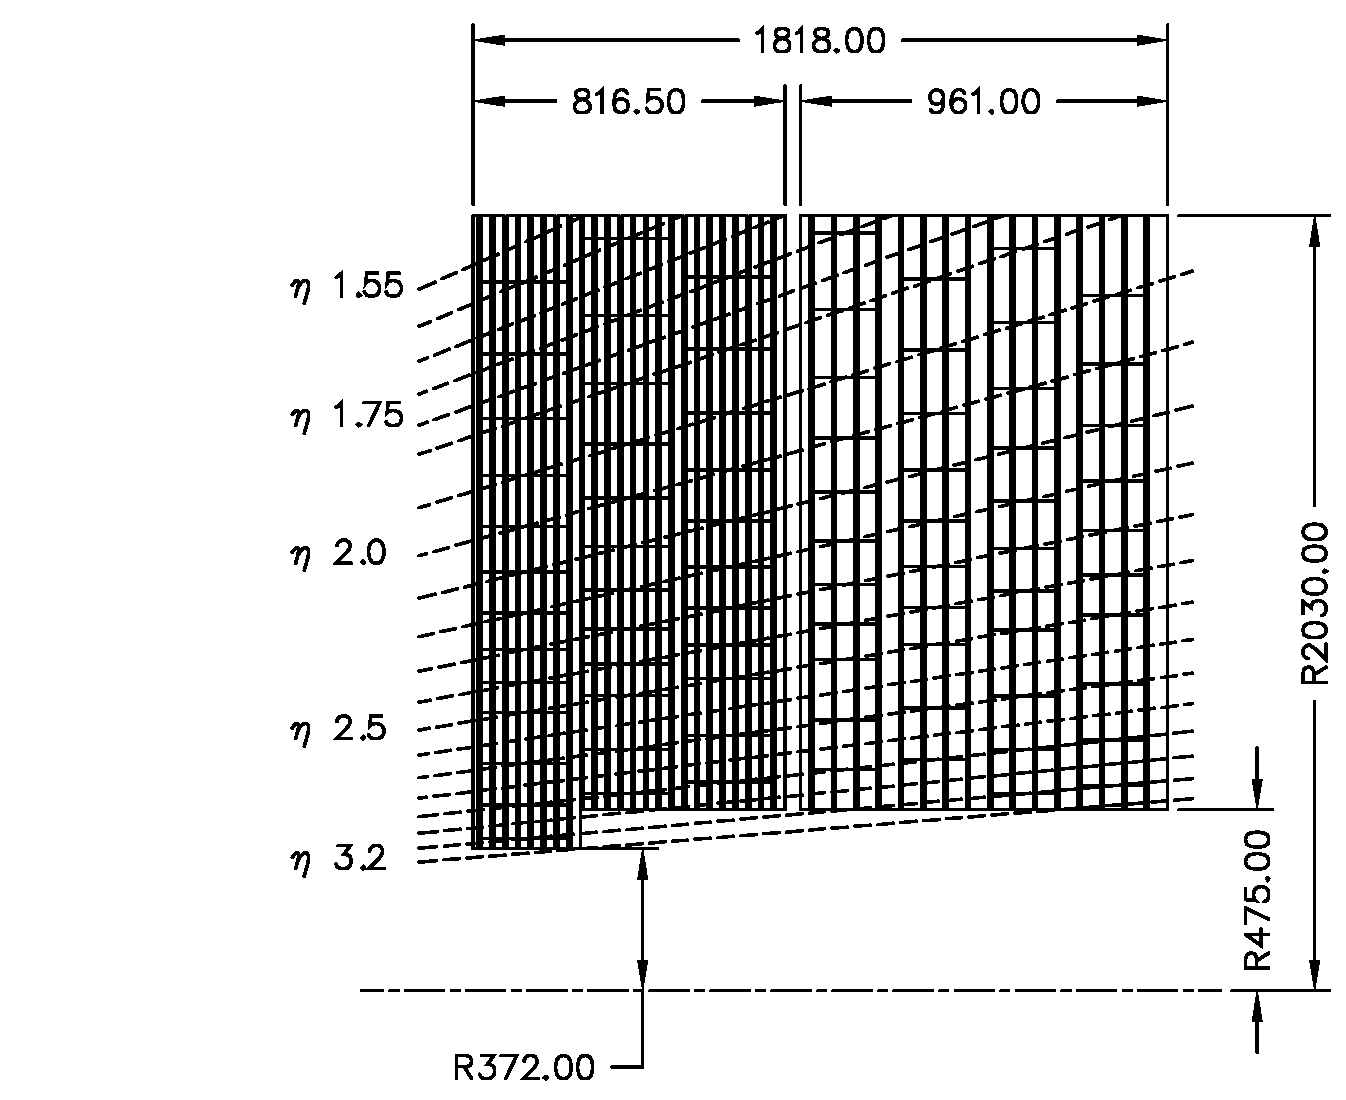
\includegraphics[width=.7\textwidth]{figures/atlas/hec.pdf}
\caption{ A schematic showing one quadrant of the 
HEC system in the $R$-$z$ plane. The dashed lines indicate
the pointing direction achieved by the segmentation of the 
readouts.  Dimensions are in mm.  }
\label{fig:atlas_hec}
\end{figure}


The HEC is designed to measure hadronic energy deposits in the 
end-cap regions from $1.5 < |\eta|< 3.2$. It uses 
copper plates as the sampling material with LAr gaps
for the active material. Two separate wheels are formed from
flat plates of copper alternating with LAr gaps further divided by electrodes for
collecting the ionization charge from the hadronic shower in the LAr.
The rear wheel is more coarse than the front wheel,
as can be seen in the schematic of \fig\ref{fig:atlas_hec}.
The electronics readout is segmented such that pointing information
can be obtained, as indicated by the dashed lines.
The maximum radial depth of the HEC is roughly $10~\lambda$.



\begin{figure}[ht] 
\centering
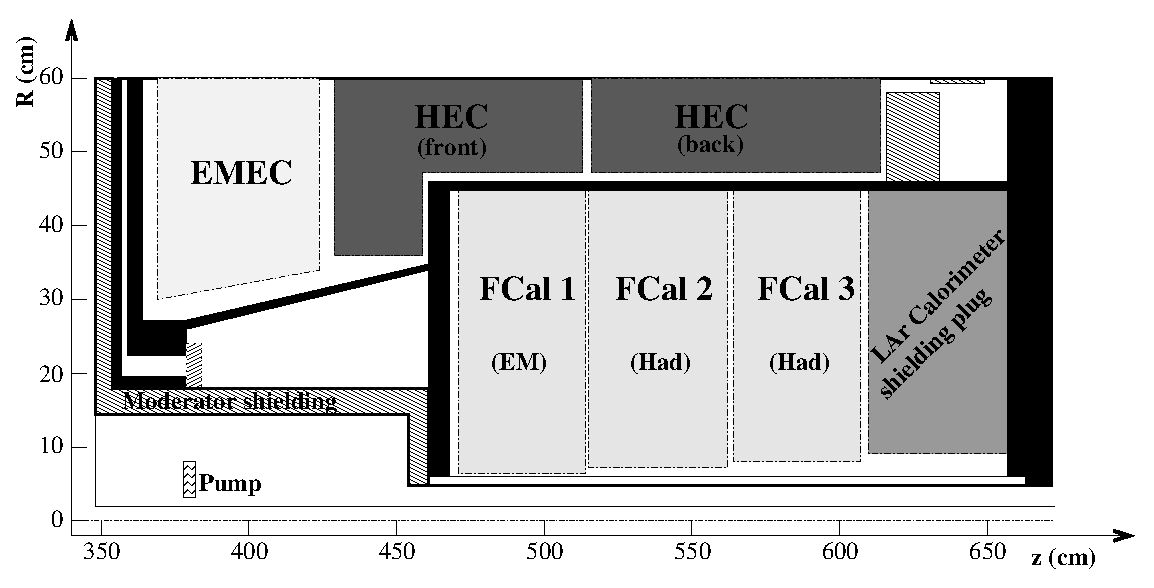
\includegraphics[width=.95\textwidth]{figures/atlas/fcal.eps}
\caption{ A schematic showing the end-cap of the ECAL,
the two HEC modules, and the three FCAL modules, as well
as additional shielding, in one
quadrant of the ATLAS detector, as viewed 
in the $R$-$z$ plane.
The $R$-direction is shown with a larger scale than in the $Z$-direction.
}
\label{fig:atlas_fcal}
\end{figure}


The FCAL is in the region of the detector nearest to the beam-line, 
where the radiation flux is highest, covering the range
from $3.1 < |\eta| < 4.9$. It is split into three cylindrical modules,
oriented as in \fig\ref{fig:atlas_fcal}, with the first 
being designed for measuring electromagnetic deposits and the other
two for hadronic deposits.
Each FCAL module is constructed from copper plates with roughly ten thousand
uniformly spaced holes drilled in the direction parallel to the beam-line.
The holes are filled with rods serving as the primary sampling material, 
with a thin LAr gap surrounding the rods serving as the active material.
The first FCAL uses copper rods to optimize for electromagnetic deposits
while the second and third FCAL modules use tungsten rods
to optimize for hadronic deposits.
The first FCAL has a radiation length of $27.6~\xzero$ and an 
interaction length of $2.66~\lambda$. Meanwhile, the interaction
length of the second and third modules is around $3.6~\lambda$.



%Shielding? Resolution and response?




\section{Muon Spectrometer}
%do i want to talk about muon reconstruction?
%definitely mention muon resolution
\label{sec:atlas_ms}

\begin{figure}[ht]
\centering
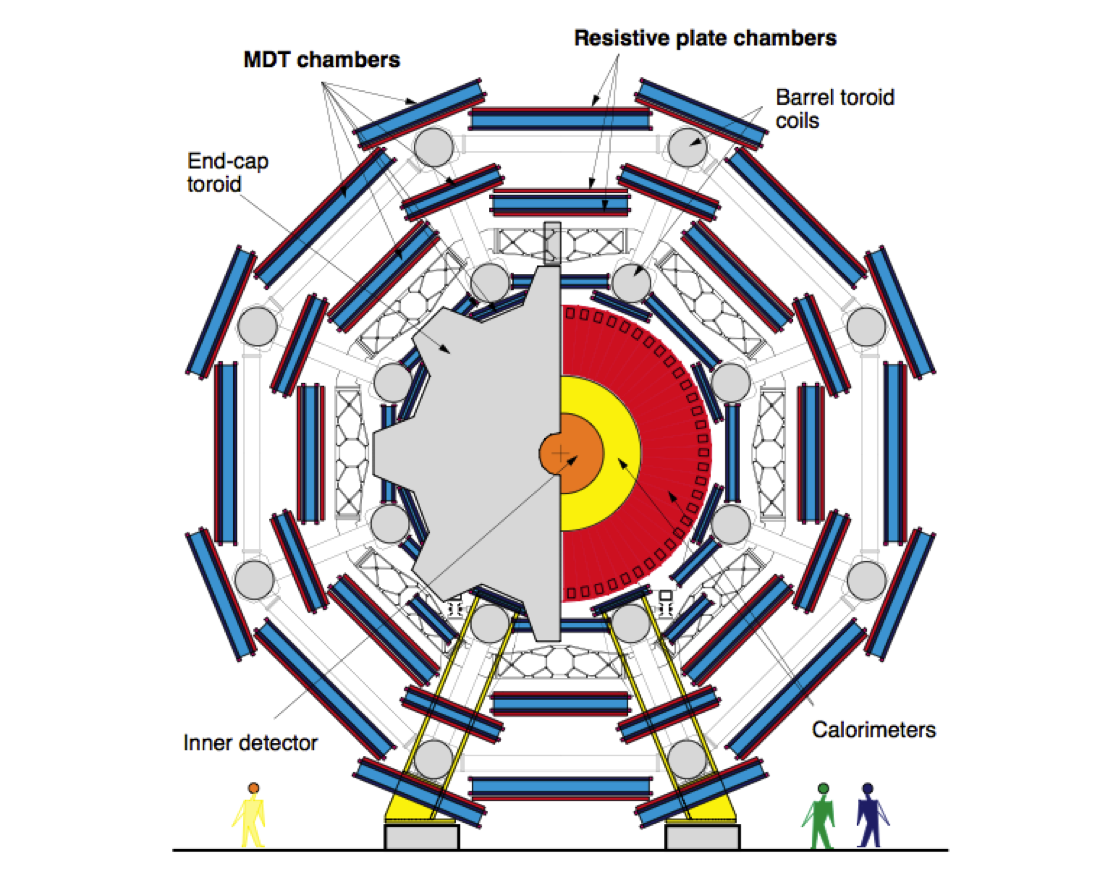
\includegraphics[width=.95\textwidth]{figures/atlas/ms_rphi}
\caption{A cross-section of the MS in the 
transverse ($r-\phi$) plane viewed from one end of the detector. 
The MDT chambers, RPCs, and
barrel and end-cap toroids of the MS system are clearly labeled.
The barrel toroid coils extend in to and out of the page while only
half of the end-cap toroid is shown to reveal the ID and calorimeter
systems.  The LHC beam pipe runs through the center.}
\label{fig:atlas_ms_rphi}
\end{figure}

\begin{figure}[ht]
\centering
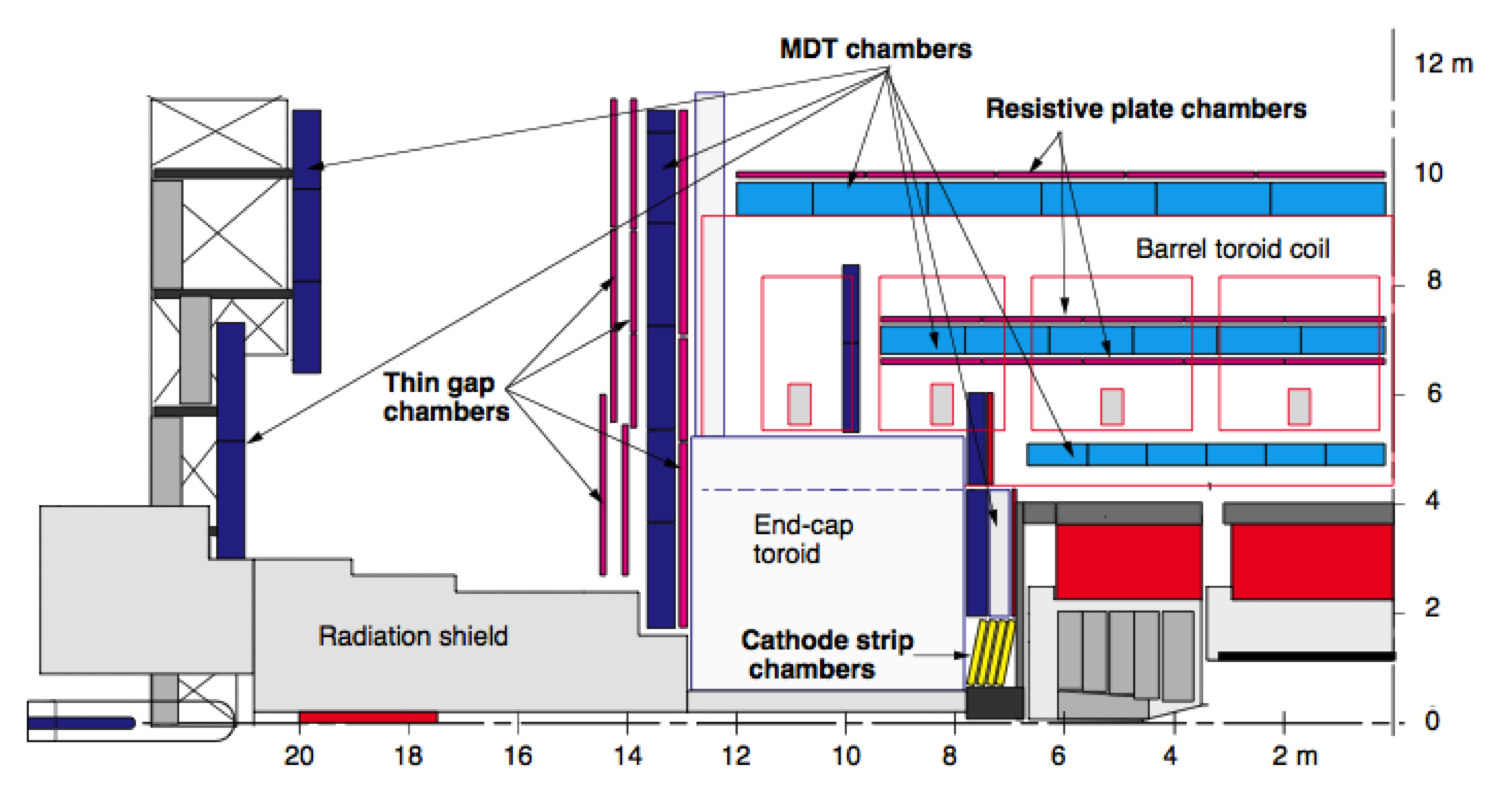
\includegraphics[width=.95\textwidth]{figures/atlas/ms_rz}
\caption{One quadrant of the MS as viewed in the $R-z$ plane. The
MDT chambers, RPCs, TGCs, CSCs are clearly indicated, as are the 
the end-cap and barrel toroids. Support structures, shielding and the calorimeter
and ID systems are also drawn. The LHC beam pipe runs from left to right
along the bottom.}
\label{fig:atlas_ms_rz}
\end{figure}

The Muon Spectrometer (MS) is the largest component of the ATLAS
detector and the component that determines its overall size. 
%The size is determined by the field strength and lever arm...
%maybe try to explain that... look in book that was taken...
It is designed to measure and identify muons as they
pass through the MS and leave the detector.
It surrounds the beam pipe, as well as the ID and calorimeter systems,
using a cylindrical geometry with a barrel and two end-caps. 
The MS is comprised of several different technologies:
Muon Drift Tubes (MDT) and Cathode Strip Chambers (CSC) are used as
precision tracking components for measurements of the muon 
trajectory, Resistive Plate Chambers (RPC) and 
Thin Gap Chambers (TGC) are used as triggering 
components with good timing resolution, 
and a toroidal magnet system is used for bending the muon trajectory 
in order to extract a momentum measurement.
A diagram of the MS in the transverse plane is shown in 
\fig\ref{fig:atlas_ms_rphi} where the MDT chambers and RPCs of the barrel
are clearly shown along with the barrel and end-cap toroids.
Another view of the MS in \fig\ref{fig:atlas_ms_rz} is displayed in
one quadrant along the axial direction which
shows the barrel and end-cap toroids, along with 
the MDT chambers in the barrel and end-cap, the RPCs in the
barrel, and the CSCs and TGCs in the end-cap.

%The physics requirements are...
\begin{figure}[ht]
\centering
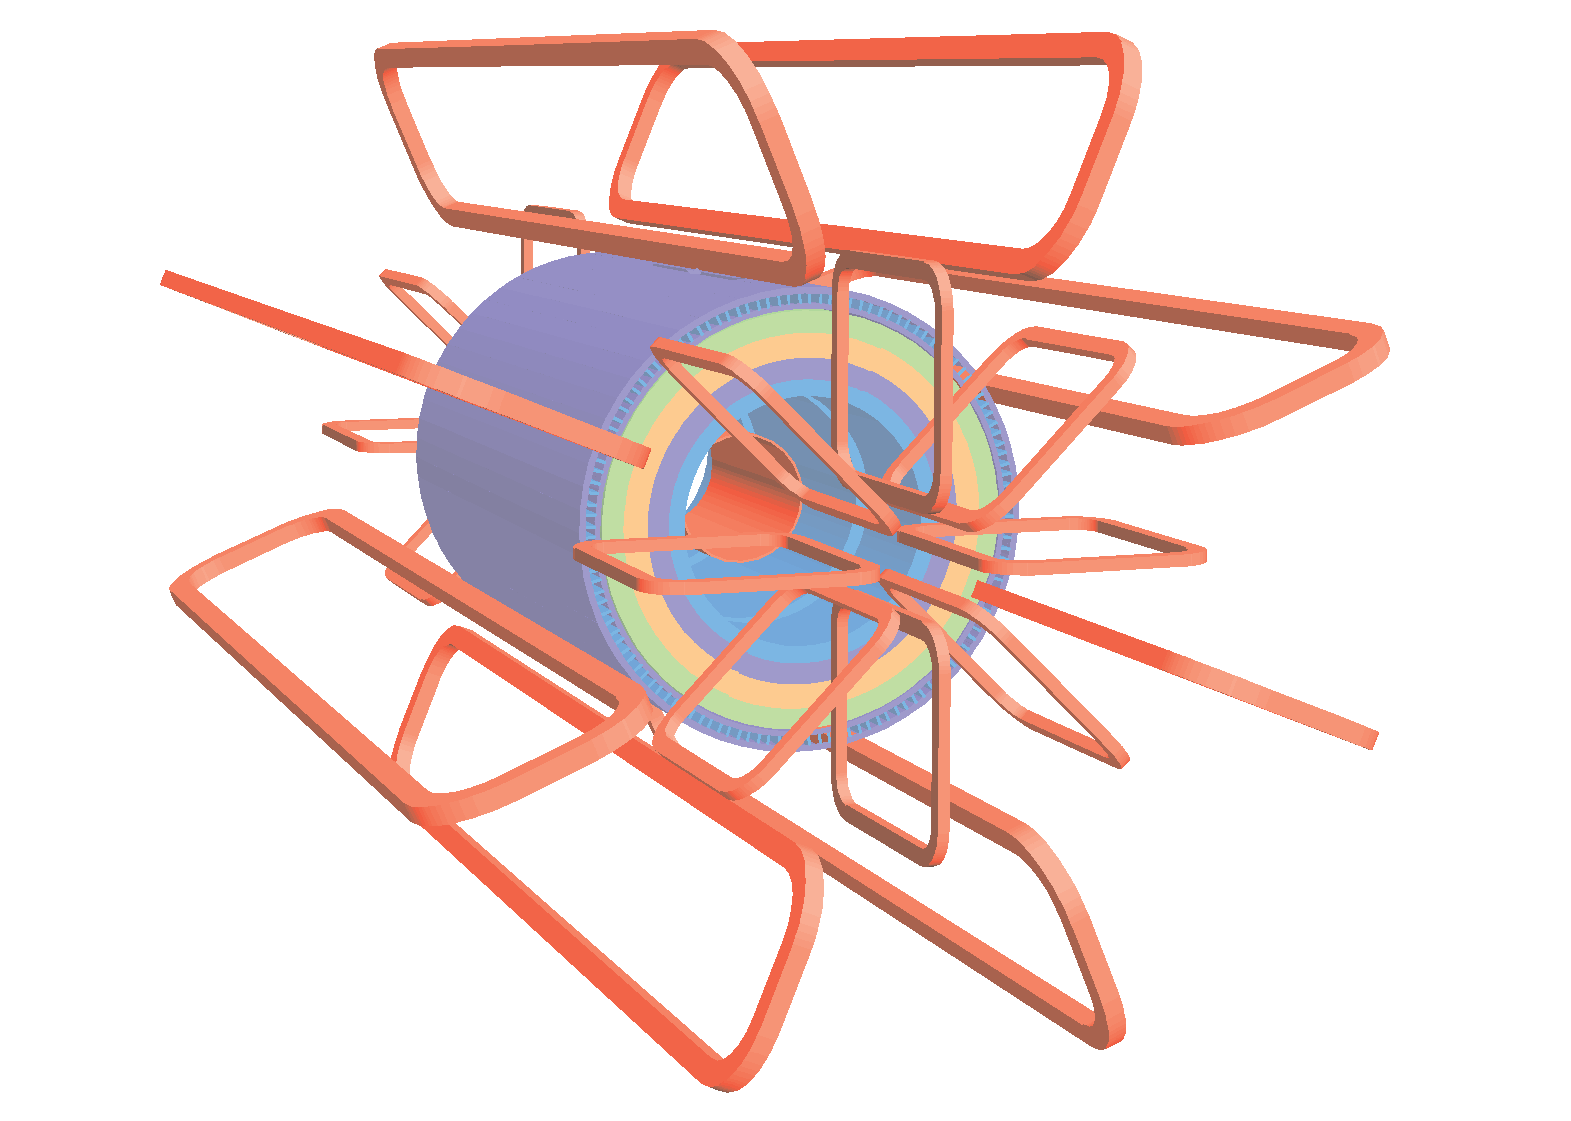
\includegraphics[width=.495\textwidth]{figures/atlas/magnet}
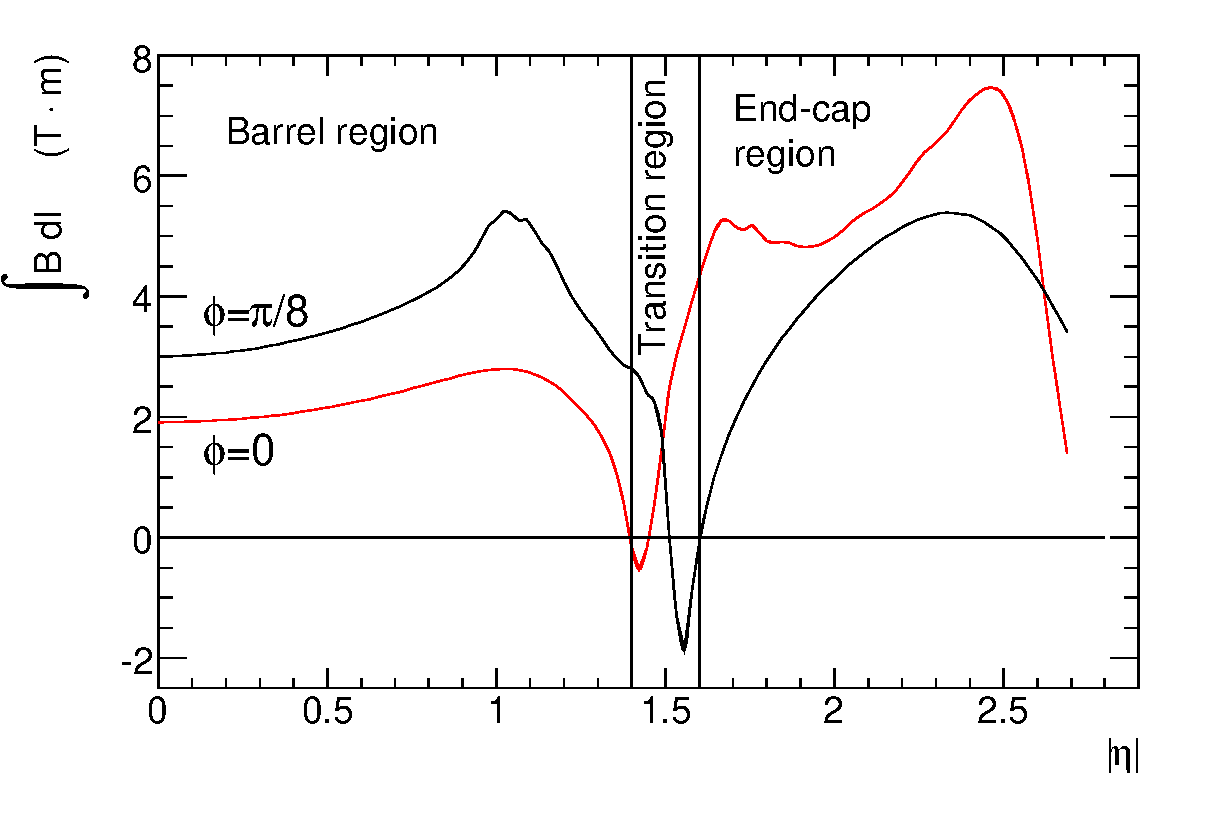
\includegraphics[width=.495\textwidth]{figures/atlas/toroid_magnet_field}
\caption{(Left) Diagram of MS toroid magnet geometry shown in red. The
tile calorimeter is also shown.
(Right) Predicted field strength of the MS magnet 
system as a function of $|\eta|$
for $\phi=0$ in red  and $\phi=\pi/8$ in black.}
\label{fig:atlas_toroid_magnet}
\end{figure}


The MS magnet system is composed of several large air-core toroids built
from superconducting coils which produce a magnetic field of 
roughly 0.5 Tesla in the barrel and 1 Tesla in the end-cap. 
The geometry of the MS magnet system is shown 
on the left of \fig\ref{fig:atlas_toroid_magnet}. In the barrel, 
eight 25 m long toroidal 
coils inside stainless-steel vacuum enclosures are placed uniformly in 
azimuth around the barrel. In the two end-caps, 
each end-cap toroid is composed of 
eight square coils (rotated with respect to the barrel toroids)
separated by supporting wedges and then surrounded in a single 
cryostat.
The resulting field is non-uniform as can be seen on the right
of \fig\ref{fig:atlas_toroid_magnet}. 
The field strength in the transverse plane is roughly zero and so is referred
to as the non-bending plane, while the $\eta$ direction is referred to as the
bending plane.
To achieve adequate momentum resolution, the resulting field must be known
precisely.
The field is measured in all directions using sensors placed throughout
the MS and shown to usually agree with predictions within a few milli-Tesla.
The field is especially non-uniform in the region from 
$1.3 < |\eta| < 1.65$, referred to as the transition region, 
where the bending power of the field actually becomes zero
for certain values of $\eta$ and $\phi$.
This results in degraded momentum resolution and poor trigger efficiencies
in this region.


\begin{figure}[ht]
\centering
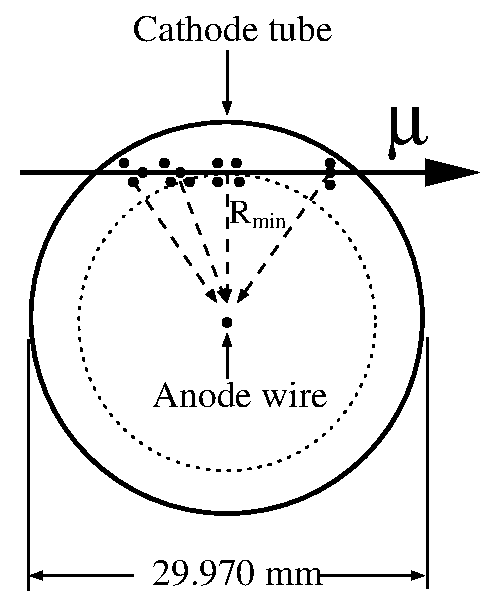
\includegraphics[width=.35\textwidth]{figures/atlas/ms_mdt_tube.eps}
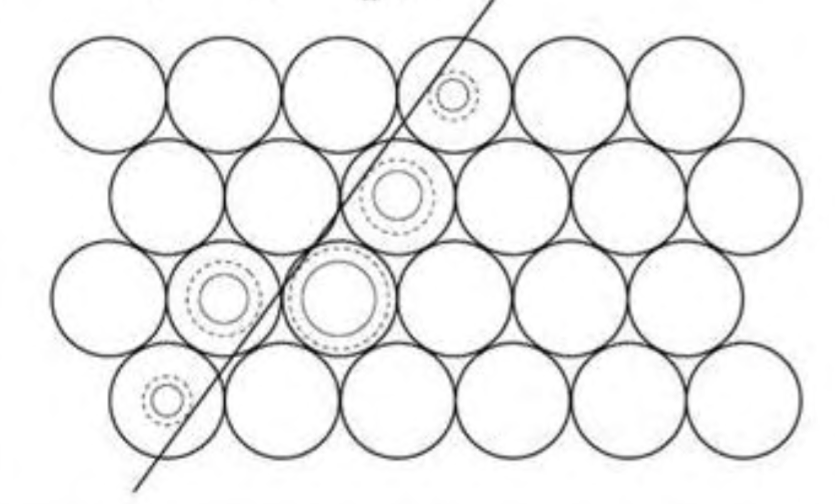
\includegraphics[width=.55\textwidth]{figures/atlas/ms_mdt_hits.png}
%ms_mdt_hits taken from http://arxiv.org/pdf/0810.3184.pdf
\caption{(Left) Cross-section of single MDT tube with muon track
passing through. Ionized electrons (black dots) collect on the anode wire
due to the applied electric field. (Right) Muon track
reconstructed from array of MDT tubes.}
\label{fig:atlas_ms_mdt}
\end{figure}



\begin{figure}[ht]
\centering
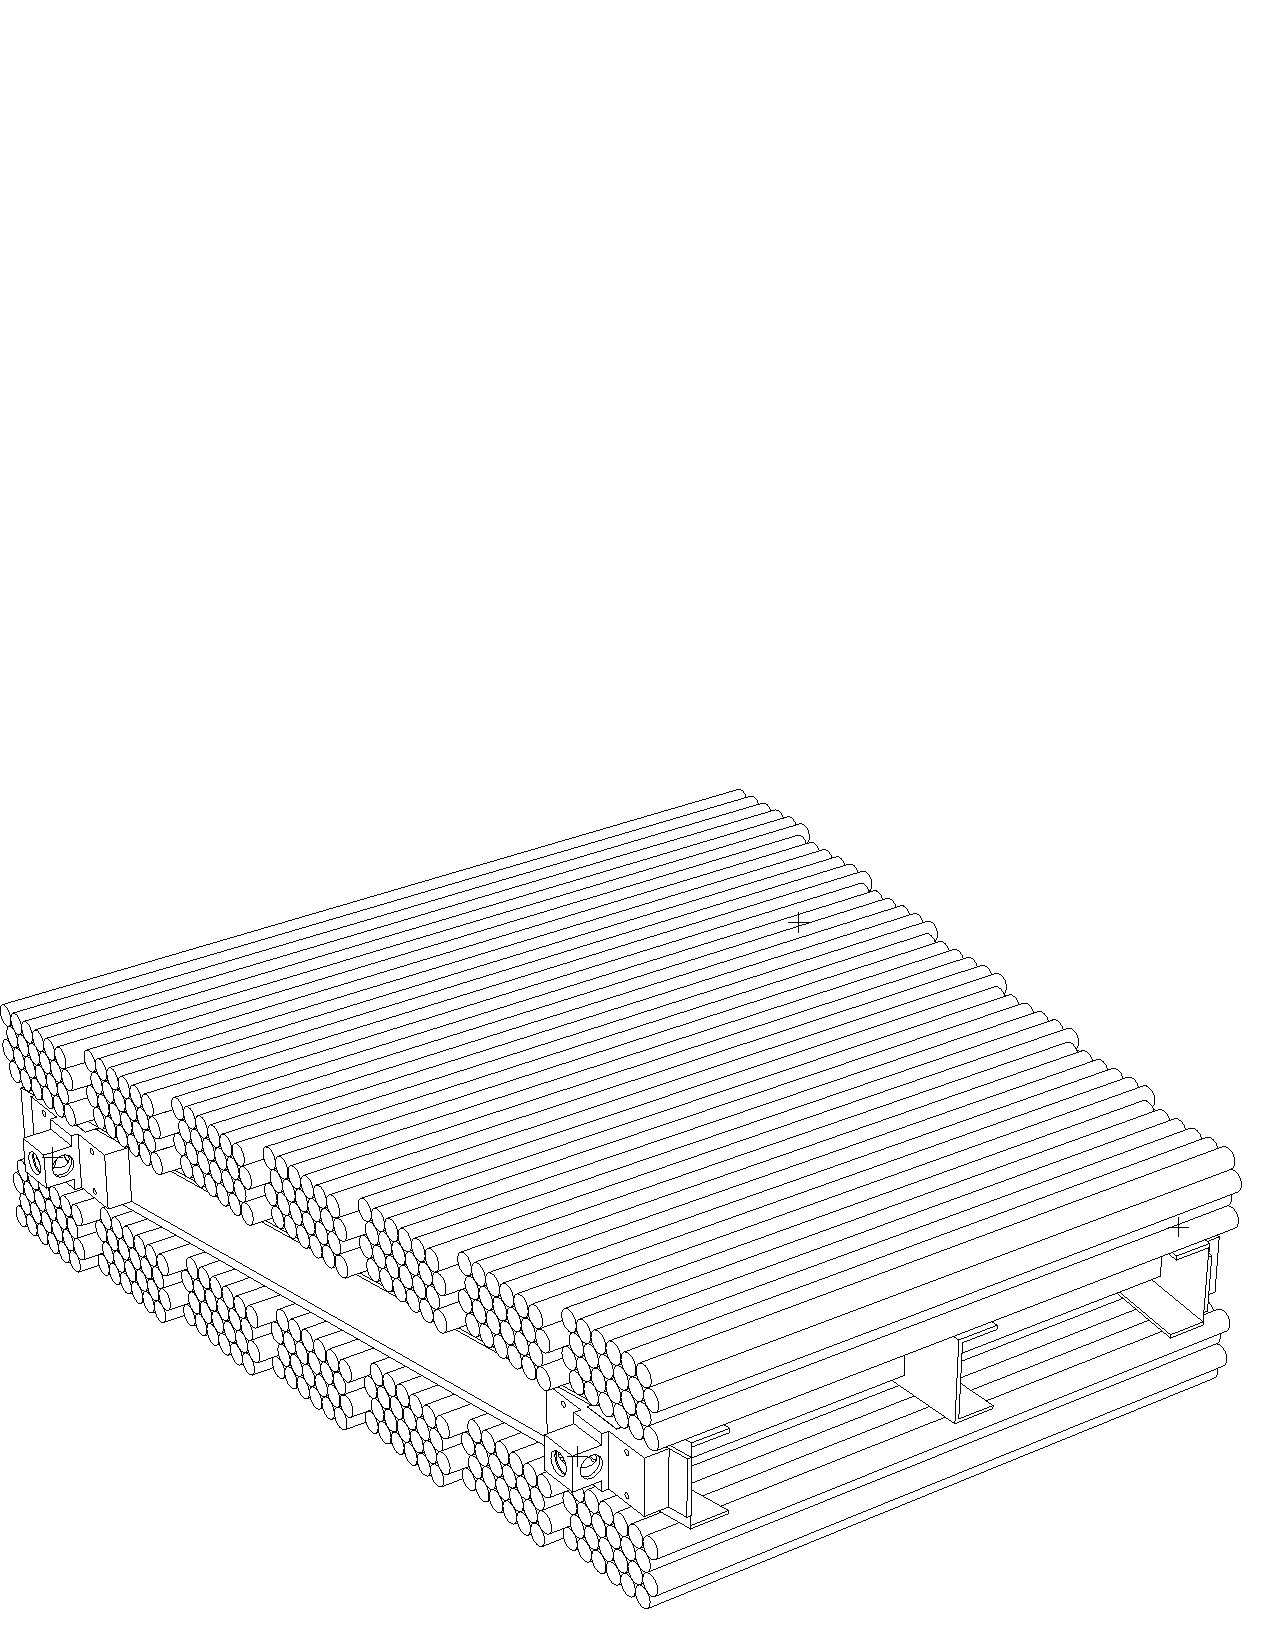
\includegraphics[width=.8\textwidth]{figures/atlas/ms_mdt_chamber.pdf}
%ms_mdt_hits taken from http://arxiv.org/pdf/0810.3184.pdf
\caption{Schematic of a single MDT chamber.}
\label{fig:atlas_ms_mdt_chamber}
\end{figure}

%figure taken from http://hedberg.web.cern.ch/hedberg/home/atlas/atlas.html

The precision tracking system has stringent requirements
on the precision of the muon trajectory measurement, 
which come from design goals on the resolution of the muon
transverse momentum measurement to be 
about 10\% at 1~\TeV.
Given the magnetic field strength in the MS, a muon 
with this momentum is expected to have a sagitta
of about $500~\mu$m in the bending plane. 
According to \eqn\eqref{eq:sagitta},
this then translates into a precision requirement of 
no more than $50~\mu$m on the sagitta.
In order to achieve this, MDT chambers are used everywhere 
in the MS from $|\eta|<2.7$ except in the inner layer of the 
end-cap from $2<|\eta|<2.7$
where the rates are too high. Here, CSCs are used instead. 
The MDT system is an arrangement of roughly 1000 MDT chambers composed
of aluminum drift tubes roughly 30 mm in diameter and a couple meters in length 
filled with a gas mixture
(Ar/CO2) and a high voltage wire (~3000 V)
running through the center. 
It was chosen as the main muon tracking system
because of its precision, simplicity, and reliability.
When a muon passes through an MDT
it ionizes the gas and electrons are collected at the wire.
The drift-time for the electron signal to collect on the wire
can be used to determine the radial distance away from the wire
at which the muon passed, like on the left of \fig\ref{fig:atlas_ms_mdt}. 
The cylindrical symmetry
of the tube is useful as the resolution is roughly flat, at around
$80~\mu$m in the bending plane, as a function
of the angle of incidence of the muon hitting the tube. 
It is not possible, however, to determine the direction
of the muon in the bending plane from just one tube.  For that reason, 
tubes are arranged together in multi-layers of 3 to 8 tubes such that 
the trajectory
can be reconstructed from matching the pattern of hits in multiple layers
to form track segments,
such as on the right of \fig\ref{fig:atlas_ms_mdt}.
A chamber is built from 2 multi-layers separated by a spacer ranging from
6 mm to 300 mm wide depending on 
the chamber, as in \fig\ref{fig:atlas_ms_mdt_chamber}.
The precision per chamber is roughly $35~\mu$m.
The long length of the MDTs means that they cannot provide a  useful measurement
in the non-bending plane.
Chambers are arranged in three concentric shells in the barrel 
at $r = $5 m, 7.5 m, and 10 m as in \fig\ref{fig:atlas_ms_rphi} 
and in several rings in the end-cap
at $|z| = $7.4 m, 10.8 m, 14 m, and 21.5 m as in \fig\ref{fig:atlas_ms_rz}.
In each shell or ring
the chambers are made to overlap in order to avoid gaps in azimuth.
Tracks are then reconstructed by interpolating between the 
track segments of the individual chambers.
Still, there are gaps, in particular around $|\eta|=0$ due to a hole for services
and due to the feet holding up the detector, seen in \fig\ref{fig:atlas_ms_rphi}.
An optical alignment system is used to monitor the MDT chambers %alignment between chambers?
for deformations. The tension of the wires can also be adjusted
to account for sag where needed. %technically only in barrel.
Despite having very good precision, the maximum drift time
can be as high as 700 ns, which is far too slow for LHC bunch identification.


\begin{figure}[ht]
\centering
\includegraphics[width=.7\textwidth]{figures/atlas/ms_csc_disk.eps}
\caption{Diagram showing the arrangement of the CSCs in the end-cap.}
\label{fig:atlas_ms_csc_disk}
\end{figure}


The CSC are used in the region of the MS closest to the interaction
point where the crossing rate of tracks 
is greater than $150$ Hz/cm$^2$, 
too high for successful operation of the MDT chambers.
The CSCs can handle up to 1000 Hz/cm$^2$
while maintaining adequate  precision in the bending plane.
A CSC is a multi-wire proportional chamber
composed of planes of cathode strips sandwiching 
a row of parallel anode wires and filled with a non-circulating gas (Ar/CO2)
in the gap.
The two planes of cathode strips are separated by 5mm
with the anode wires running directly between the two planes.
A signal is induced on the cathode strips due to an avalanche
of electrons from the ionizing muon collecting on the anode wire.
The two planes of cathode strips are segmented in orthogonal directions
providing measurements in both the bending and non-bending planes of the detector. 
A CSC is composed of four of these layers, each giving separate $\eta$ and
$\phi$ measurements.
The resolution in the bending plane is roughly 60 $\mu$m
while the coarser segmentation in the non-bending plane 
results in a  resolution of  roughly 5 mm.
Two rings are formed from the chambers such that the anode wires
point radially and there are no gaps in $\phi$, as
can be seen in \fig\ref{fig:atlas_ms_csc_disk}. The rings are positioned
at roughly $|z|=7.5$ m. The rectangular symmetry of the individual channels
results in a degradation of the resolution based on the angle of incidence.
This is resolved by titling the chambers slightly toward the interaction point.
The signal pulse height can be used to match the tracks
if multiple tracks are present in a CSC in a given event. This 
is useful in the high occupancy environment near the beam-line.
The small separation between cathode strips results in 
a short electron drift time allowing for a good
timing resolution of about 7 ns per layer.

%optical alignment? Resolution?
\begin{figure}[tb]
\centering
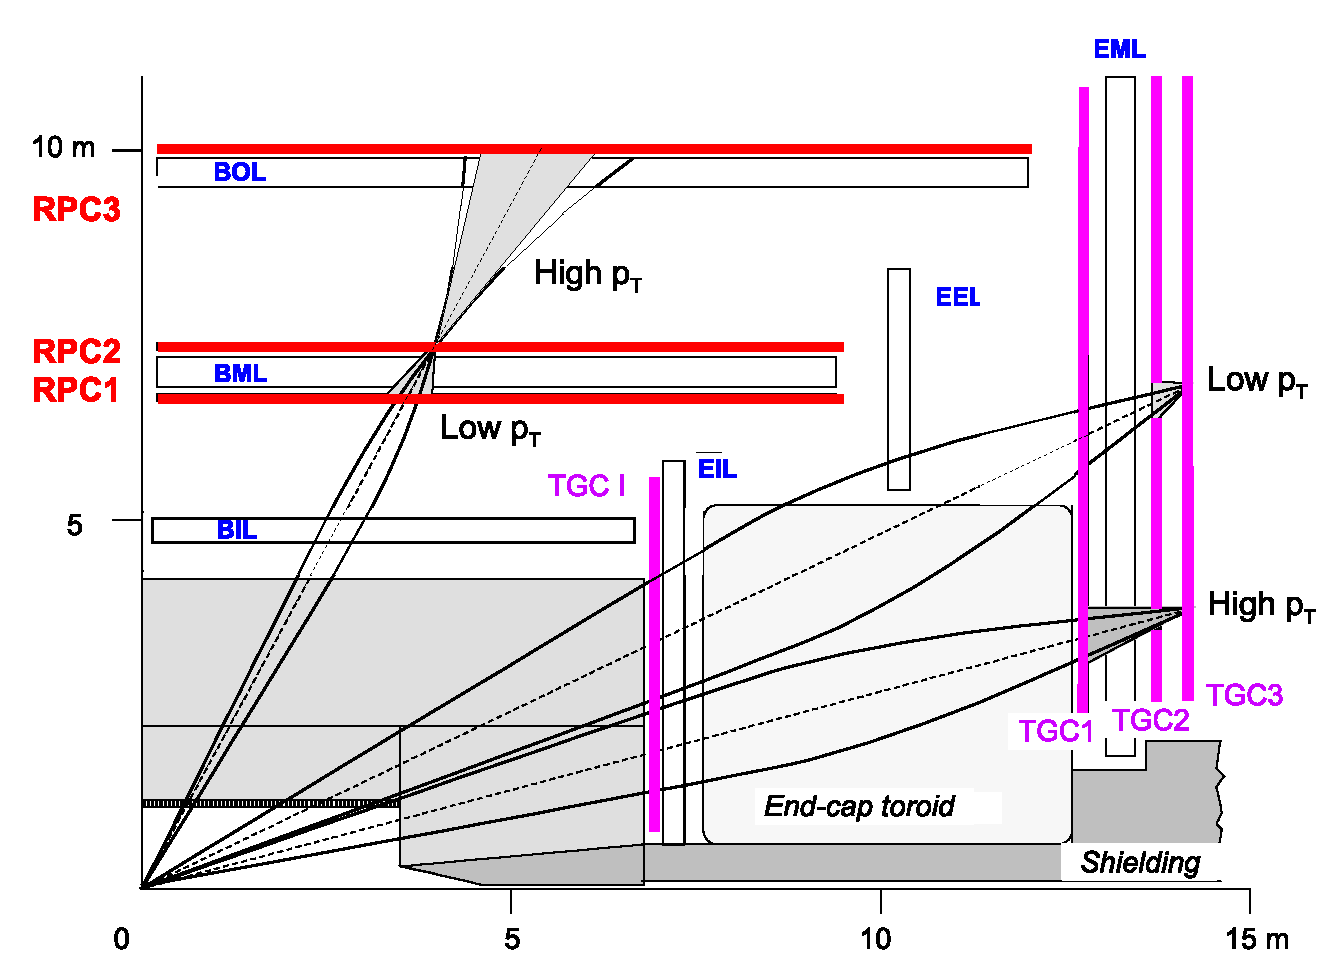
\includegraphics[width=.95\textwidth]{figures/atlas/ms_trigger_layout.eps}
\caption{Layout of the trigger components for one quadrant
in the $r-z$ plane. RPC and TGC chambers are clearly labeled. Possible
muon trajectories are seen for low and high \pt~roads formed
by the trigger algorithm (see \sec\ref{sec:atlas_trigger}).}
\label{fig:atlas_ms_trigger_layout}
\end{figure}

The triggering system in the MS is designed to be able
to identify muons coming from individual bunch crossings of the LHC
and to discriminate them based on their position and \pt~in the region
$|\eta|<2.4$. This information
is then used to trigger on high \pt~muons, as 
described in \sec\ref{sec:atlas_trigger}.
The individual bunch crossings of the LHC are designed to 
be separated by only 25 ns, as described in Chapter \ref{sec:lhc}.
Thus, the system must be able to resolve individual tracks 
with a time resolution of this size.
%(what exactly is the design reqs?).
To distinguish high \pt~muons from straight-track neutral particles 
or from curved-track low-momentum charged particles, the 
system must be able to measure the sagitta of the 
trajectory in the toroidal magnetic field, though not necessarily
with the same precision as in the precision tracking system.
Furthermore, to distinguish individual tracks, position measurements
must be performed in both the bending and non-bending planes.
The measurement in the non-bending plane is also used to complement
the measurements of the bending plane from the MDT chambers.
RPCs are used in the barrel region
from $|\eta|<1.05$ and TGCs in the end-cap from $1.05 < |\eta|<2.4$.
The layout of the MC triggering system can be seen in the diagram
in \fig\ref{fig:atlas_ms_trigger_layout}. 
The RPCs are parallel electrode-plate detectors which use no wires.
A single RPC layer consists of 
resistive plates aligned in parallel and separated by 2 mm 
with a gas mixture (primarily $\textrm{C}_2\textrm{H}_2\textrm{F}_4$)
in the gap. An electric field of 4.9 kV/mm is applied between 
the plates which results in electron avalanches forming in the gas
along the track.
This gives a signal pulse time resolution of about 5 ns.
The pitch of the individual plates is 23 mm in $\eta$ and 35 mm in $\phi$.
A single RPC consists of two such layers.  Three concentric shells 
are formed from the RPCs around the beam line 
at about $r = $ 6.5 m, 7.5 m, and 10 m
as in \fig\ref{fig:atlas_ms_trigger_layout}.
The separation between the inner and outer layers 
allows for a discrimination of muons with $9 < \pt < 35~\GeV$
while the separation between the inner and middle layers allows for 
discrimination of low-\pt~muons with $6 < \pt < 9~\GeV$.
%Space resolution...maybe put sqrt(12) formula? look up to be sure.


The TGCs are multi-wire proportional chambers, similar to the CSCs.
In a single TGC layer, the cathodes are 
separated by 2.8 mm and the wire-to-wire pitch
is 1.8 mm.  A high voltage of 2900 V is applied to the anode wires
resulting in a quasi-saturated electron avalanche in the gas 
mixture (CO2/n-pentane) due to incident tracks.
The small wire-to-wire pitch and high voltage result in a good 
timing resolution for the signal pulse. The resulting
signal pulse resolution is dependent on the angle-of-incidence
of the incoming track, but still results in a signal width
within 25 ns for about 99\% of tracks.
TGC chambers are built from either two or three layers. 
The TGC chambers are then arranged in rings such that they overlap
in azimuth to eliminate gaps.
The TGC rings are arranged as in 
\fig\ref{fig:atlas_ms_trigger_layout}
with a ring of two-layer TGCs placed in front of the end-cap MDT inner
layer at about $|z|=7$ m, 
a ring of three-layer TGCs placed in front of the end-cap MDT
middle layer at around $|z|=13 $m, and two rings of 
two-layer TGCs placed just behind
the end-cap MDT middle layer at around $|z|=14$ m.
%pt resolution and performance?



\section{Trigger}
\label{sec:atlas_trigger}

The very small design bunch spacing 
of 25 ns (40.08 MHz) at the LHC, combined with the average raw digitized event size
of around 1 Megabyte, means that to record every collision
would require a bandwidth of around 40 Terabytes per second, far surpassing
the capabilities of modern hard-disks. Thus, recording every collision
is clearly untenable. Fortunately, the type of collisions of interest at the LHC 
(high \pt~leptons and jets, high \met) are sufficiently rare 
that most collisions can be filtered out before recording. 
This is accomplished by using a so-called ``triggering'' system, 
that quickly analyzes coarse information about the collision
and only records those collisions deemed to be of interest.
The trigger is implemented in stages. The 40.08 MHz collisions are
first passed to a custom electronics Level-1 (L1) trigger, designed
to reduce the rate to below 75 kHz; it is then  passed to the 
relatively simple software-based selection in the 
Level-2 (L2) trigger, designed to reduce the rate
to no more than 3.5 kHz; finally, it is passed to the third stage,
called the Event Filter (EF), which uses a more complex software-based 
selection similar to the offline selection, reducing the 
rate to below 200 Hz. The L2 and EF triggers are referred to together
as the High-Level Trigger (HLT). This results in a much more reasonable 
bandwidth for writing the data of about 0.2 Gigabytes per second.
To achieve these goals requires careful design and also (sometimes difficult)
choices about what types of collisions to keep.  This is discussed in more
detail below. 

The L1 trigger system is designed to use reduced granularity information
from the calorimeter and muon systems with custom electronics
to make on-the-fly decisions about interesting physics objects.
The inner detector is not used at L1.
Information about muons is taken from the muon track measurements of 
the RPC and TGC components of the MS
as described in \sec\ref{sec:atlas_ms}. This information is 
used to build coarse trajectories called roads. The width of the road
is used to make one of a few possible \pt~cuts on the 
trajectory in the range of roughly $6<\pt<35~\GeV$. 
Meanwhile, information from the 
calorimeters is limited to coarse trigger ``towers'' mostly of dimension
$0.1 \times 0.1$ in $\Delta\eta \times \Delta\phi$.
Look-up-tables are used to quickly identify the transverse energy 
from the road.
This is then summed using several sliding window algorithms to identify 
high \pt~electrons and photons, hadronically decaying taus, jets, large \met,
or large \et. 
In both the L1 muon and calorimeter triggers, special care is taken
to account for object multiplicities and to not double count physics objects. 
One important challenge is that the 
calorimeter signals and muon time of flight are slow enough\footnote{One
of the rare instances where the speed of light can be considered slow!}
that the signals from multiple bunch crossings occur in the detector
simultaneously.  Thus, each signal must be carefully synchronized with 
the bunch crossing from which it came.  
This must also account for the latency of the trigger itself, which
is around 2 $\mu$s.  The information
from the L1 muon and calorimeter triggers are passed to the Central
Trigger Processor which makes a decision about whether or not to pass
the event to the L2 trigger.  It does this by testing 
a number of possible conditions (for example, is there at least one
muon with $\pt > 15 \GeV$?) and then taking the logical OR of all of
these conditions.

The L2 trigger takes as input so-called ``Regions-of-Interest'' (RoI)
which are provided by the L1 trigger (for example, a cluster of 
trigger towers or a muon road). By restricting to RoIs,
the L2 trigger need only consider about 1-2\% of the 
total event\footnote{There are some instances of the L2 trigger
using the full event, but this is used sparingly.}. 
The L2 trigger runs simplified reconstruction algorithms in the RoIs 
on a computer processing farm. 
A number of  more detailed conditions are tested
to investigate 
if an interesting physics object really is present in the RoI.
If so, those conditions which returned a positive result are 
passed to the EF.

The EF is also run on a processor farm, but runs reconstruction algorithms
which are very similar to those run during offline reconstruction.
In many cases the EF will run on the full event. The conditions
that were satisfied in L1 and L2 determine which algorithms and conditions
are run in the EF.  The list of conditions tested at the EF (and 
how they are connected to the L1 and L2) is referred to as the trigger menu.
The trigger menu can have hundreds of items.
Given the finite bandwidth of the trigger, the trigger menu
must be carefully chosen as not all are created equal. Some 
trigger items can take up a lot of bandwidth, some not.
Some might be considered essential, some obscure.
To mitigate this problem, some trigger items might be ``pre-scaled'',
meaning they are only kept some random fraction of the time.
In the end, the trigger menu is an important statement about the physics
priorities of the collaboration.
If any of the trigger menu items are satisfied they are finally written to disk.

%plots of trigger menu?

%trigger performance?











%\section{LUCID?}

\chapter{The first search for \wwwlll}
\label{sec:www}
%this can have all of the details of the analysis

%1 paragraph (pg) on why this is important
%1 pg laying out the analysis design



%I'm assuming these are abbreviated here:
%MC - Monte Carlo
%LO - Leading-Order
%NLO - next-to-leading-order
%SFOS - Same-Flavor Opposite-Sign

%Introduction to WWW analysis
The first measurement of the $WWW$ production process
is sought by using a dataset containing 20.3 \ifb~of integrated luminosity
collected from the LHC at an energy of \energy~in 2012.
In addition to being the first study of this particular process,
it is also the first study to search for a final state with more 
than two massive gauge bosons, and one of the first studies
to search for aQGCs.
%assuming aQGCs will be defined earlier
The total \xsec for this process is expected
to be roughly $224$~femtobarns, as determined using 
\madgraph~\cite{MadGraph}. If measured, it 
would be one of the smallest \xsec measurements
within ATLAS. %with about 64\% coming from associated Higgs production.
For this search, the \www~process is studied in the 
so-called ``fully leptonic'' decay channel
where each $W$ boson decays leptonically (excluding $\tau$ lepton decays).
As can be seen in \fig\ref{fig:branching_fractions},
this decay channel occurs only about 1\% of the time;
the rest of the time
at least one of the $W$ bosons decays hadronically.
%due to this jets problem
While the branching fraction is small,
this channel has a smaller background than those 
that include hadronic $W$ decays.
As a result, the fully leptonic channel
is one of the most sensitive channels
for studying this process.


The data is studied in a ``signal region'' where the signal is most prominent
with respect to the background.  This region is primarily characterized
by having three high \pt~leptons ($e$ or $\mu$), with additional
requirements determined using an optimization procedure.
To understand the data in this region we must model 
both the signal and the backgrounds that fall into it.
The signal is modeled using Monte Carlo (MC) simulation 
while the backgrounds are modeled using a combination of MC
simulation and data-driven techniques.
Prior to the measurement, each important background is 
studied in a ``control region'', where there is little to no signal contamination,
to ensure that the backgrounds are described accurately.
In the signal region, the agreement of the data 
with the signal plus background prediction is determined using 
a ``cut-and-count'' approach where the total number of data 
events observed in the signal region is compared to the expected number
of events from the model.
A fit to the data is performed using a profile likelihood
with the relative normalization of the signal as 
the parameter of interest and with statistical and systematic 
uncertainties treated as nuisance parameters.
%more detail? citations?
From this fit, the measured signal \xsec and uncertainty,
the sensitivity of the data to the signal 
under the background only hypothesis,
and limits on new physics in an effective field theory 
are extracted.



                                                                                







\section{Data and Simulation Samples}
\subsection{Data}
\label{sec:subsection_data}



This analysis is based on the study of the full proton-proton collision
data from the LHC in 2012. After quality requirements, the amount 
of data used in this analysis corresponds to 
an integrated luminosity of \lumi.
The uncertainty on the integrated luminosity is $2.8\%$ 
following the same methodology as in \cite{Aad:2013ucp}.
%from Van-der-Meer scans taken throughout 2012.
%read this citation.
The data are selected after requiring that at least one
of a series of single lepton triggers passed during data taking, 
specifically, one of the following:
either an electron trigger 
requiring at least one isolated
electron with $\pt>24$~\GeV~, an electron trigger requiring
at least one (possibly non-isolated) electron 
with $\pt>60$~\GeV, a muon 
trigger requiring at least one isolated muon with $\pt>24$~GeV,
or a muon trigger requiring at least one 
(possibly non-isolated) muon with $\pt>36$~GeV.


\subsection{Simulation samples}
%%Do I need to talk about Monte Carlo showering, 
%%hadronization and reconstruction?
%%A general discussion of Monte Carlo could go here

An important tool for the modelling of physics processes
that are/could be produced at the LHC is Monte Carlo simulation (MC).
MC relies on random sampling to connect the matrix element formulations
derived from quantum mechanical pertubation theory into 
actual predictions for the results of proton-proton collisions
at the LHC.
The prediction of a single collision from the MC represents
one possible outcome of the proton-proton collision, with all of the 
products of the hard-scattering and their four-momenta.
This result can be passed through additional MC simulation to describe
hadronization and the soft products of the collision e.g. photon radiation.
Finally, these products are passed through a detailed 
simulation of the ATLAS detector built in \geant~\cite{Agostinelli:2002hh}
so that the same reconstruction algorithms
can be applied as in the data.
This sampling is repeated many times to populate the 
distribution of possible
outcomes. Dedicated MC programs are provided by theorists for 
different processes and to different orders in pertubation theory,
sometimes with different treatments.
Details of the different processes simulated from MC and their
treatment are presented below.




\subsubsection{Signal Processes}
\label{sec:signal}


%%%
%If I'm going to include this, I better read up on it.
%%%
%The production \xsec without Higgs contribution has been calculated 
%to $\mathcal{O}(\alpha_s)$  corrections in Ref~\cite{Binoth:2008kt}.
%$\mathcal{O}(\alpha_s)$ corrections, Higgs boson exchange and spin 
%correlations of $W$ bosons lepton decay are also available
%~\cite{Campanario:2008yg}.  

The SM $WWW$ signal processes are implemented in the Monte
Carlo generator \vbfnlo~\cite{Arnold:2011wj,Arnold:2012xn},
which can generate partonic events at leading-order (LO) in QCD with
next-to-leading-order (NLO) cross-sections, 
and in \madgraph~\cite{MadGraph}, which can generate
partonic events at NLO  with NLO cross-sections. 
The partonic events are further processed 
by \pythiaeight~\cite{Sjostrand:2007gs} and \photos~\cite{Golonka:2005pn} 
to add effects of beam remnant interactions and initial and 
final state radiation. 
SM parameters, such as the Higgs mass,
must be provided to the MC generators as input. 
The underlying event
parameters are set in \pythiaeight~ using the ATLAS tune 
of AU2\cite{atlas:2011zja}.
The MC generators must also be provided an appropriate PDF.
The PDF used  in the LO \vbfnlo~generation is
the LO CTEQ6L1~\cite{Pumplin:2002vw} PDF set;
CT10 NLO~\cite{guzzi:2011sv}
is used in the NLO \vbfnlo~cross-section calculation.
The PDF used in the NLO \madgraph~generation 
and \xsec~calculation is CTEQ6L1 
but this is re-weighted to CT10 NLO using a k-factor of 1.08 to 1.10.
Since the MC generators are computed to finite order in perturbation
theory, renormalization and factorization scales must be chosen.
The renormalization and factorization scales are dynamically
set to the $WWW$ invariant mass in the \vbfnlo~samples; they 
are set to a fixed scale equal to the $Z$ mass in \madgraph.
The \vbfnlo~samples are restricted to leptonic decays of the $W$~bosons
where each lepton has a \pt~of at least 5~\GeV. The \madgraph~
samples include all decays of the $W$~boson, with a requirement 
that jets have a a \pt~of at least 10~\GeV~ but with no requirement
on the \pt~of leptons.
They are compared in a common fiducial phase space,
described in more detail in \sec\ref{sec:fiducial}.
The \vbfnlo~ and \madgraph~samples handle interference 
between $WH\rightarrow WWW(*)$ 
and on-shell $WWW$ production at LO, but \madgraph~is not
able to do this at NLO. As a result, the NLO \madgraph~samples
are split into sepearate samples of 
on-shell \www~ and $WH\rightarrow WWW(*)$ production.
Both sets are further split by the \www~charge mode.
For each sample, the \xsecs are summarized in \tab\ref{tab:signal_xsec} 
in their full phase space and in the common fiducial phase space.
The fiducial \xsecs are observed to be nearly the same
between the two generators.
This serves as a good check of the understanding of the 
signal process. The \madgraph~\xsecs are used throughout the 
remainder of the analysis.

%Do I need to describe the k-factors?
%It would be nice to also add some distributions from Rivet comparing
%the two at truth level.


%Describe the pdf uncertainty calculation.
%what about renormalization and factorization scales




%\begin{table}[ht]
%\centering
%\input{tables/SignalSMParameters.tex}
%\caption{List of the most relevant SM parameters used as input to the 
%signal MC generation.}
%\label{tab:signal_sm_parameters}
%\end{table}


\begin{table}[ht]
\centering
\input{ tables/combination/signal_xsec.tex}
\caption{Inclusive and common fiducial cross-sections at NLO 
for \vbfnlo~and \madgraph~samples. 
The sum of the inclusive \xsecs are different
because of the different branching fractions in the two cases. 
The sum of the fiducial cross-sections, however, are expected to be similar because
they are computed for the same phase space, as described in \sec\ref{sec:fiducial}.
Only statistical uncertainties are shown.}
\label{tab:signal_xsec}
\end{table}


%%%%
%soud I show the dependence on scales here?
%%%%
%The dependencies of the 
%$\xsecs on the choices of scales have been studied in the two
%references~\cite{Binoth:2008kt,Campanario:2008yg}. 

% The production at LO is a pure electroweak process. The
% NLO correction brings in $\alpha_s$ which actually makes the cross
% sections more sensitive to the choices of scales. 
%It has been pointed
%out that a jet veto should reduce the scale dependence. 

%The $W$ boson is short lived, so one must study its decay products.
%As already mentioned, the focus of this analysis is on the final state 


%need to also show the MadGraph parameters
%maybe rephrase so that I can discuss both in parallel
%get generation parameters from semi-leptonic note
%report both sets of cross-sections here
%include updated info on cross-sections and PDFs 

\begin{figure}[ht!]
\centering
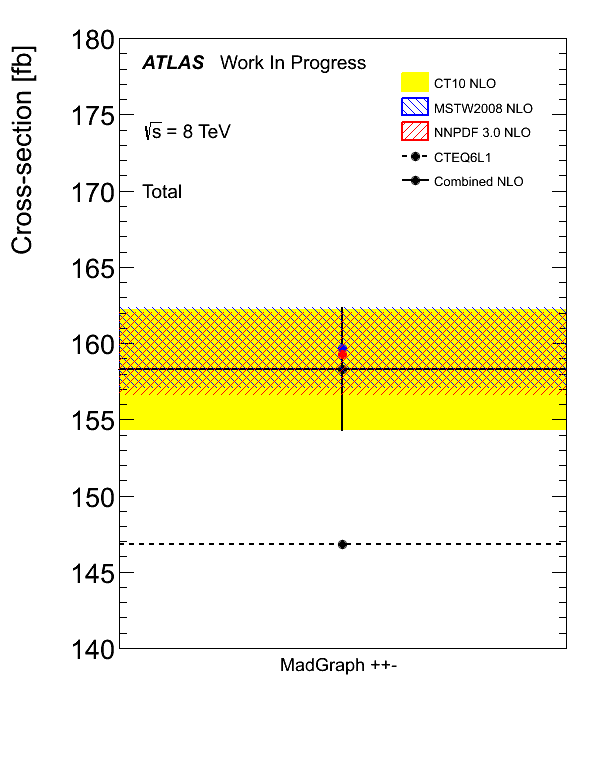
\includegraphics[width=.35\columnwidth]{figures/pdf/MADppm_total_cteq6l1.png}
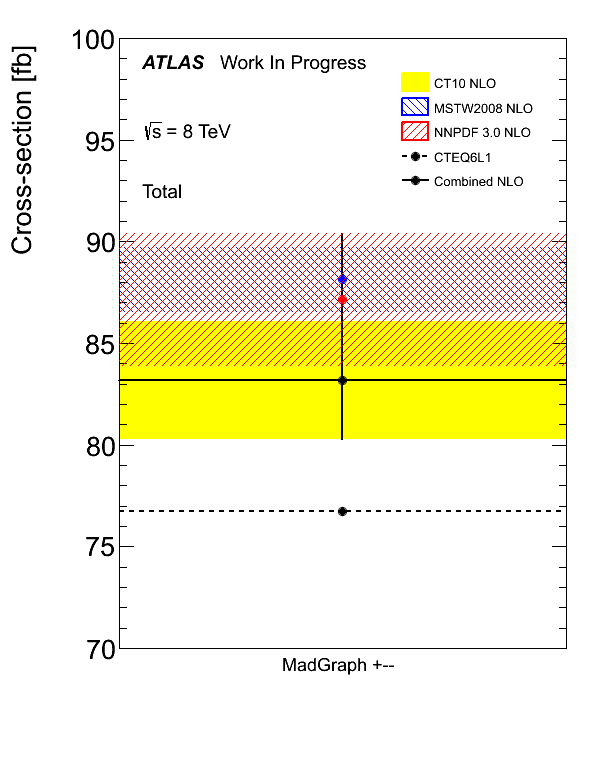
\includegraphics[width=.35\columnwidth]{figures/pdf/MADpmm_total_cteq6l1.png}
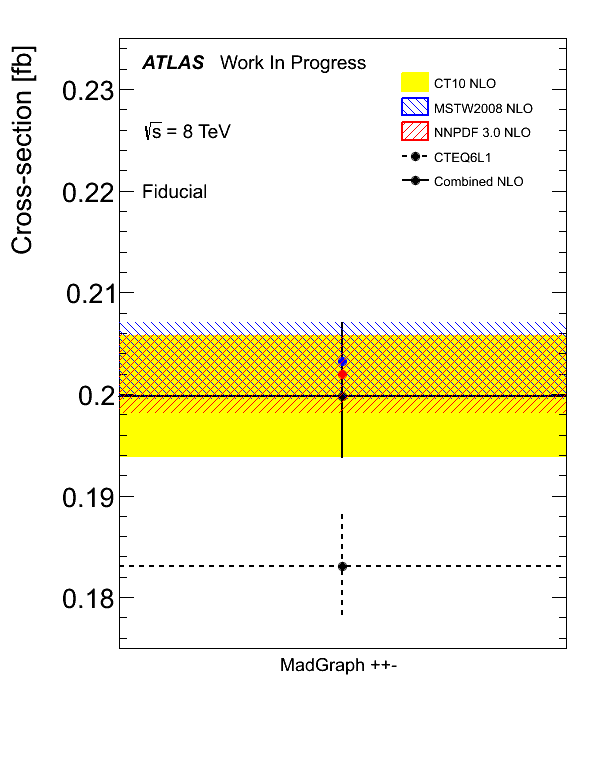
\includegraphics[width=.35\columnwidth]{figures/pdf/MADppm_fiducial_cteq6l1.png}
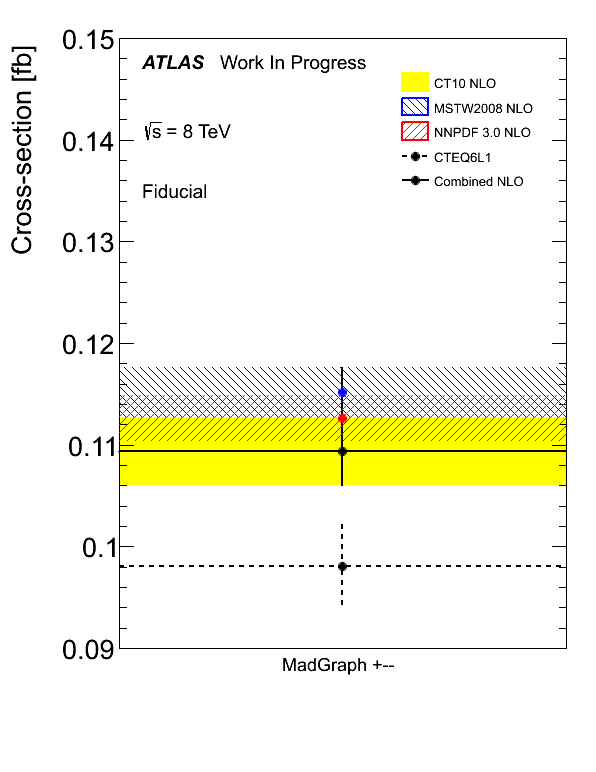
\includegraphics[width=.35\columnwidth]{figures/pdf/MADpmm_fiducial_cteq6l1.png}
\caption{The signal cross-sections for different PDFs along with their
uncertainties are shown on the {\sc MadGraph} $WWW$ signal samples
for the total $WWW$ phase space and branching fraction for
the $W^{+}W^{+}W^{-}$ (top left) and $W^{+}W^{-}W^{-}$ (top right)
charge modes
and in the fiducial region for $W^{+}W^{+}W^{-}$ (bottom left) 
and $W^{+}W^{-}W^{-}$ (bottom right).
The bands show the PDF uncertainty for CT10 NLO (solid yellow),
MSTW 2008 NLO (hashed blue), and NNPDF 3.0 NLO (hashed red). The
solid line shows the envelope of all uncertainty bands used as the final
PDF uncertainty estimate. The central value of CT10 NLO is taken as the
central value of the estimate.
The dashed-line shows the cross-section and 
statistical uncertainty for the CTEQ6L1
pdf sets used in the original generation step.}
\label{fig:signal_pdf_unc}
\end{figure}

\begin{table}[ht!]
\centering
\begin{tabular}{c|c|c}
\hline
 & \multicolumn{2}{c}{PDF Uncertainty}\\
 & $W^{+}W^{+}W^{-}$ & $W^{+}W^{-}W^{-}$ \\
\hline
\hline
Total & $+2.58\%~-2.51\%$ &  $+8.69\%~-3.47\%$ \\
Fiducial & $+3.64\%~-3.00\%$ & $+7.57\%~-3.08\%$ \\
\hline
\end{tabular}
\caption{Summary of PDF uncertainties estimated on NLO {\sc MadGraph} cross-sections
in both the fiducial and total phase space.}
\label{tab:pdfunc}
\end{table}

Uncertainties on the signal prediction mainly come from the choice of PDF, 
the inherent PDF uncertainty, and the renormalization and factorization
scales, as described in \sec\ref{sec:pdf}.
The uncertainty due to the choice of PDF is derived for the {\sc MadGraph} 
cross-sections following a modified version of the pdf4lhc
\cite{Botje:2011sn} recommendations.  The resulting 
uncertainty is shown separately for the two different charge modes
in both the fiducial and the inclusive phase
space in Table~\ref{tab:pdfunc}.
The uncertainty is determined by comparing three different PDFs:
CT10 NLO~\cite{Lai:2010vv}, MSTW2008 NLO~\cite{Martin:2009iq}, 
and NNPDF 3.0 NLO~\cite{Ball:2014uwa}. 
This comparison is presented in \fig\ref{fig:signal_pdf_unc}.  
Symmetric 68\% CL uncertainties 
are determined for CT10 NLO and MSTW 2008 NLO using the 68\% CL 
set provided for MSTW directly and the 90\%CL set for CT10 after
scaling down by 
a factor of 1.645 in order to approximate a 68 \% CL uncertainty. 
The uncertainty of the NNPDF 3.0 NLO PDF set is 
determined by using the standard deviation of the distribution 
of 101 MC PDFs provided in the PDF set; the nominal value is taken
from the mean of the same PDFs.  
The CT10 NLO PDF central value is used as the nominal 
value of the final estimate.
The final PDF uncertainty on that estimate is
taken as the envelope of the uncertainty bands for all three PDF sets.  



The uncertainty on the factorization and renormalization scales are 
determined by varying each of them independently up or down by 
a factor of two. 
The effect of these variations on the cross-sections
as compared to the nominal
are shown separately for the two different charge 
modes in \tab~\ref{tab:scaleVariation}.
The symmetric uncertainty is then determined by taking the maximum 
variation for each charge mode, 
namely, 2.62\% for $W^+W^+W^-$ and 2.53\% for $W^-W^+W^-$. 

\begin{table}[ht!]
    \centering
\begin{tabular}{cc|ccc}
\hline
& \backslashbox{$\mu_F$}{$\mu_R$}     & $\frac{1}{2}M_{WWW}$ & $M_{WWW}$ &  $2M_{WWW}$ \\
\cline{2-5}
\multirow{3}{*}{\Wp\Wp\Wm} &$\frac{1}{2}M_{WWW}$ & 2.62\% & -0.14\% & -2.11\% \\
%\cline{2-5}
&$M_{WWW}$ & 2.13\% & 0 & -2.41\% \\
%\cline{2-5}
&$2M_{WWW}$ & 1.56\% & 0.24\% & -2.42\% \\
\hline
\hline
& \backslashbox{$\mu_F$}{$\mu_R$}     & $\frac{1}{2}M_{WWW}$ & $M_{WWW}$ &  $2M_{WWW}$ \\
\cline{2-5}
\multirow{3}{*}{\Wm\Wp\Wm} &$\frac{1}{2}M_{WWW}$ & 1.91\% & 1.38\% & -2.00\% \\
%\cline{2-5}
&$M_{WWW}$ & 1.61\% & 0 & -2.53\% \\
%\cline{2-5}
&$2M_{WWW}$ & 1.25\% & -1.05\% & -2.12\% \\
\hline
\end{tabular}
\caption{The relative variation of the NLO cross sections corresponding 
to different choices of factorization and renormalization 
scales for the \Wp\Wp\Wm and \Wm\Wp\Wm  processes. }
\label{tab:scaleVariation}
\end{table}

The signal cross-sections and uncertainties are thus determined to be 
\begin{equation}
\sigma^{\textrm{Total}}_{\textrm{Theory}}= 241.47\pm0.13 ~(\textrm{Stat.}) ~^{+10.33}_{-6.08} ~(\textrm{PDF}) ~\pm 6.3 ~(\textrm{Scale}) ~\textrm{fb} %uncertainty?
\end{equation}
for the inclusive \xsec and
\begin{equation}
\label{eq:fiducial_theory}
\sigma^{\textrm{Fiducial}}_{\textrm{Theory}}= 309.2\pm7.2 ~(\textrm{Stat.}) ~^{+15.05}_{-8.36} ~(\textrm{PDF}) ~\pm 8.0 ~(\textrm{Scale}) ~\textrm{ab} %uncertainty?
\end{equation}
for the fiducial cross-section.


%should i include this
%The analysis considers events with three leptons ($e$ or $\mu$) in the final state. The contributions from events in which $W$ bosons decay to $\tau$'s, and the $\tau$'s sequentially decay to $e$ or $\mu$ should be included and is expected to be 40\% of total yield of the 3-lepton final state.  


\subsubsection{aQGC signal}
\label{sec:aqgc_signal}
\input{www_aqgc_signal}






















\newpage

\subsubsection{Backgrounds samples}
\label{sec:subsection_datasets_MC}

Only processes containing 3 or more prompt
leptons ($WZ$, $ZZ$, $t\bar{t}V$, $VVV$), or 2 leptons and an 
isolated photon ($Z+\gamma$) are estimated using MC simulation 
samples in this analysis. The other processes are estimated from 
data as this will be explained in Section~\ref{sec:backgrounds_estimation}. 
The samples listed in this section and containing less than 3 prompt leptons 
have been used for preliminary or dedicated studies, but are not used for 
the determination of the final results. The MC samples are pass through the 
GEANT4~\cite{Agostinelli:2002hh} simulation~\cite{Aad:2010ah} of the ATLAS 
detector and reconstructed in the same way as the data.

The diboson and triboson samples are listed in Table~\ref{tab:sample_bkg_dibosons}. The triboson samples other than the signal, \textit{ie}: $ZWW^{*}$ and $ZZZ^{*}$ were generated using the MadGraph~\cite{Alwall_madgraph} generator, hadronized through the Pythia6~\cite{PYTHIA} parton shower, with the AUET2B~\cite{ATL-PHYS-PUB-2011-009} tunes and the CTEQ6L1~\cite{Pumplin:2002vw} PDF set. The $Z\gamma$ samples were generated with the Sherpa~\cite{sherpa} generator and the CT10~\cite{Guzzi:2011sv} PDF set. The $W\gamma$ samples were generated with the AlpGen~\cite{ALPGEN} generator, hadronized through JIMMY~\cite{Jimmy}, with the AUET2C~\cite{ATL-PHYS-PUB-2011-009} tunes and the CTEQ6L1 PDF set. Other diboson samples ($WW$, $WZ$, $ZZ$) were obtained using the Powheg~\cite{Alioli:2008gx,Nason:2004rx,Frixione:2007vw,Alioli:2010xd} generator, hadronized through the Pythia8~\cite{Sjostrand:2007gs} parton shower, with the AU2~\cite{atlasmctunes} tunes and the CT10 PDF set. Dedicated high-stat $WZ$ and $ZZ$ samples were generated to increase the statistics in all the signal region used in this analysis. They were obtained requesting the presence of 3 leptons with $\pt>7~\GeV$.

The dibosons samples where the production is due to loop induced process or Double Parton Scattering (DPS) processes are summarized in Table~\ref{tab:sample_bkg_dibosons_gg2DPI}. The loop induced processes were generated using the gg2ZZ~\cite{Binoth:2008pr} and gg2WW~\cite{Binoth:2006mf} generators, hadronized using JIMMY, with the AU2 tunes and the CT10 PDF set. The DPS processes were generated with the AU2 tunes and the CTEQ6L1 PDF set. The cross section of these processes have been evaluated for the ATLAS same sign WW analysis~\cite{Aad:2014zda}, as this will be explained in Section~\ref{sec:bkg_DPS}.

Single boson processes are summarized in Table~\ref{tab:sample_bkg_Zjets} for the $Z+$jets samples and in Table~\ref{tab:sample_bkg_wjets} for the $W+$jets samples. The $Z+$jets samples were generated with the Sherpa generator and the CT10 PDF set. Low mass Drell-Yan samples were not simluated using the GEANT4 simulation, but with the AF2 simulation, however dedicated scale factors are applied for these samples, when they are used, in the analysis. The $W+$jets samples were generated with the AlpGen generator, hadronized through JIMMY, with the AUET2C tunes and the CTEQ6L1 PDF set.

Samples containing top quarks are summarized in Table~\ref{tab:sample_bkg_top}. $t\bar{t}$ events were generated using the MCatNLO\cite{MCatNLO} generator, hadronized through JIMMY with the CT10 PDF set. Single top samples in the s-channel and in the $Wt$ channel were generated using MCatNLO hadronized through JIMMY with the CT10 PDF set. Single top samples in the t-channel were generated using AcerMC\cite{Kersevan:2004yg}, hadronized using PYTHIA6 with the AUET2B tunes and the CTEQ6L1 PDF set. Finally $t\bar{t}V$ processes were generated using the MadGraph generator, hadronized through the Pythia6 parton shower, with the AUET2B tunes and the CTEQ6L1PDF set.


 % the $Z+jets$ samples in Table~\ref{tab:sample_bkg_Zjets}, the $W+jets$ in Table~\ref{tab:sample_bkg_wjets}, and samples containing top quarks in Table~\ref{tab:sample_bkg_top}.

When $Z+$jets and $Z+\gamma$ samples are used simultaneously, an overlap removal procedure must be used to avoid double counting of FSR events. Events containing an FSR photon with $E_{T}>10~\GeV$ are explicitely vetoed out from the $Z+$jets sample. The algorithm used is the same as what was developped in the $8~\TeV$ ATLAS $WZ$ analysis~\cite{Anger:1663539}.


\begin{table}[ht!]
  \centering
  \begin{footnotesize}
\begin{tabular}{c|c|c|c|c|c|c}
\hline
    &  &  & Cross-Section &  & Event filter  \\
  Sample  & Generator & Sample type & [pb] & k-factor &  efficiency  & used in signal region\\
\hline \hline
167007 & MadGraphPythia & ZWWStar lllnulnu  &  0.0015546  &  1  &  1 & Yes \\
167008 & MadGraphPythia & ZZZStar nunullll  &  0.00033239  &  1  &  1 & Yes \\
145161 & Sherpa & eegammaPt10  &  32.26  &  1  &  1 & Yes \\
145162 & Sherpa & mumugammaPt10  &  32.317  &  1  &  1 & Yes \\
%146430 & AlpgenJimmy & Wgamma Np0 & 230.09 & 1.15 & 1 & No \\
%146431 & AlpgenJimmy & Wgamma Np1 & 59.343 & 1.15 & 1 & No \\
%146432 & AlpgenJimmy & Wgamma Np2 & 21.469 & 1.15 & 1 & No \\
%146433 & AlpgenJimmy & Wgamma Np3 & 7.1032 & 1.15 & 1 & No \\
%146434 & AlpgenJimmy & Wgamma Np4 & 2.1224 & 1.15 & 1 & No \\
%146435 & AlpgenJimmy & Wgamma Np5 & 0.46612 & 1.15 & 1 & No \\
146436 & AlpgenJimmy & Wgamma Np0 & 229.88 & 1.15 & 0.31372 & No \\
146437 & AlpgenJimmy & Wgamma Np1 & 59.518 & 1.15 & 0.44871 & No \\
146438 & AlpgenJimmy & Wgamma Np2 & 21.39  & 1.15 & 0.54461 & No \\
146439 & AlpgenJimmy & Wgamma Np3 & 7.1203 & 1.15 & 0.62974 & No \\
126928 & PowhegPythia8& WpWm ee  &  0.62  &  1.0  &  1 & No  \\
126929 & PowhegPythia8& WpWm me  &  0.62  &  1.0  &  1 & No  \\
126930 & PowhegPythia8& WpWm te  &  0.62  &  1.0  &  1 & No  \\
126931 & PowhegPythia8& WpWm em  &  0.62  &  1.0  &  1 & No \\
126932 & PowhegPythia8& WpWm mm  &  0.62  &  1.0  &  1 & No \\
126933 & PowhegPythia8& WpWm tm  &  0.62  &  1.0  &  1 & No \\
126934 & PowhegPythia8& WpWm et  &  0.62  &  1.0  &  1 & No \\
126935 & PowhegPythia8& WpWm mt  &  0.62  &  1.0  &  1 & No \\
126936 & PowhegPythia8& WpWm tt  &  0.62  &  1.0  &  1 & No \\

185813 & PowhegPythia8& ZZ 4e mll4 TriLeptonFilter & 0.07677 & 1 & 0.57204 & Yes \\
185814 & PowhegPythia8& ZZ 2e2mu mll4 TriLeptonFilter & 0.1757 & 1 & 0.49893 & Yes \\
185815 & PowhegPythia8& ZZ 2e2tau mll4 TriLeptonFilter & 0.1757 & 1 & 0.086032 & Yes \\
185816 & PowhegPythia8& ZZ 4mu mll4 TriLeptonFilter & 0.07677 & 1 & 0.58293 & Yes \\
185817 & PowhegPythia8& ZZ 2mu2tau mll4 TriLeptonFilter & 0.1757 & 1 & 0.087166 & Yes \\
185818 & PowhegPythia8& ZZ 4tau mll4 TriLeptonFilter & 0.07677 & 1 & 0.0076557 & Yes \\

181471 & Sherpa & $ZZ*\rightarrow eeee$  $m_{Z,1} > 4$~GeV, $m_{Z,2} < 4$~GeV  & 2.8286 & 0.880 & 1.0 & No \\
181472 & Sherpa & $ZZ*\rightarrow ee\mu\mu$ $m_{Z,1} > 4$~GeV, $m_{Z,2} < 4$~GeV  & 2.34503 & 0.880 & 1.0 & No \\
181473 & Sherpa & $ZZ*\rightarrow ee\tau\tau$ $m_{Z,1} > 4$~GeV, $m_{Z,2} < 4$~GeV  & 1.59326 & 0.880 & 1.0 & No \\
181474 & Sherpa & $ZZ*\rightarrow \mu\mu ee$ $m_{Z,1} > 4$~GeV, $m_{Z,2} < 4$~GeV  & 0.48613 & 0.880 & 1.0 & No \\
181475 & Sherpa & $ZZ*\rightarrow \mu\mu\mu\mu$ $m_{Z,1} > 4$~GeV, $m_{Z,2} < 4$~GeV  & 0.50835 & 0.880 & 1.0 & No \\
181476 & Sherpa & $ZZ*\rightarrow \mu\mu\tau\tau$ $m_{Z,1} > 4$~GeV, $m_{Z,2} < 4$~GeV  & 0.42288 & 0.880 & 1.0 & No \\
181477 & Sherpa & $ZZ*\rightarrow \tau\tau ee$ $m_{Z,1} > 4$~GeV, $m_{Z,2} < 4$~GeV  & 0.00403 & 0.880 & 1.0 & No \\
181478 & Sherpa & $ZZ*\rightarrow \tau\tau\mu\mu$ $m_{Z,1} > 4$~GeV, $m_{Z,2} < 4$~GeV  & 0.00401 & 0.880 & 1.0 & No \\
181479 & Sherpa & $ZZ*\rightarrow \tau\tau\tau\tau$ $m_{Z,1} > 4$~GeV, $m_{Z,2} < 4$~GeV  & 0.00411 & 0.880 & 1.0 & No \\


% 126937 & PowhegPythia8& ZZ 4e mll4 2pt5  &  0.0735  &  1.0  &  0.90765 \\
% 126938 & PowhegPythia8& ZZ 2e2mu mll4 2pt5  &  0.1708  &  1.0  &  0.82724 \\
% 126939 & PowhegPythia8& ZZ 2e2tau mll4 2pt5  &  0.1708  &  1.0  &  0.58278 \\
% 126940 & PowhegPythia8& ZZ 4mu mll4 2pt5  &  0.0735  &  1.0  &  0.91241 \\
% 126941 & PowhegPythia8& ZZ 2mu2tau mll4 2pt5  &  0.1708  &  1.0  &  0.58725 \\
% 126942 & PowhegPythia8& ZZ 4tau mll4 2pt5  &  0.0735  &  1.0  &  0.10604 \\
126949 & PowhegPythia8& ZZllnunu ee mll4  &  0.168  &  1  &  1 & No \\
126950 & PowhegPythia8& ZZllnunu mm mll4  &  0.168  &  1  &  1 & No \\
126951 & PowhegPythia8& ZZllnunu tt mll4  &  0.168  &  1  &  1 & No \\
185795  &  PowhegPythia8 &  WmZ 3e mll0p25 TriLeptonFilter  &  0.9655  &  1  &  0.051928 & Yes \\
185796  &  PowhegPythia8 &  WmZ e2mu mll0p4614 TriLeptonFilter  &  0.6326  &  1  &  0.073874  & Yes \\
185797  &  PowhegPythia8 &  WmZ e2tau mll3p804 TriLeptonFilter  &  0.1125  &  1  &  0.012544  & Yes \\
185798  &  PowhegPythia8 &  WmZ mu2e mll0p25 TriLeptonFilter  &  0.9687  &  1  &  0.054302  & Yes \\
185799  &  PowhegPythia8 &  WmZ 3mu mll0p4614 TriLeptonFilter  &  0.6479  &  1  &  0.071268  & Yes \\
185800  &  PowhegPythia8 &  WmZ mu2tau mll3p804 TriLeptonFilter  &  0.1125  &  1  &  0.01258  & Yes \\
185801  &  PowhegPythia8 &  WmZ tau2e mll0p25 TriLeptonFilter  &  0.9687  &  1  &  0.012075  & Yes \\
185802  &  PowhegPythia8 &  WmZ tau2mu mll0p4614 TriLeptonFilter  &  0.6326  &  1  &  0.01664 & Yes \\
185803  &  PowhegPythia8 &  WmZ 3tau mll3p804 TriLeptonFilter  &  0.1108  &  1  &  0.0034037  & Yes \\
185804  &  PowhegPythia8 &  WpZ 3e mll0p25 TriLeptonFilter  &  1.416  &  1  &  0.053051 & Yes  \\
185805  &  PowhegPythia8 &  WpZ e2mu mll0p4614 TriLeptonFilter  &  0.9421  &  1  &  0.075904  & Yes \\
185806  &  PowhegPythia8 &  WpZ e2tau mll3p804 TriLeptonFilter  &  0.1755  &  1  &  0.013867 & Yes  \\
185807  &  PowhegPythia8 &  WpZ mu2e mll0p25 TriLeptonFilter  &  1.412  &  1  &  0.055296 & Yes  \\
185808  &  PowhegPythia8 &  WpZ 3mu mll0p4614 TriLeptonFilter  &  0.9572  &  1  &  0.073362 & Yes  \\
185809  &  PowhegPythia8 &  WpZ mu2tau mll3p804 TriLeptonFilter  &  0.1755  &  1  &  0.013891 & Yes \\
185810  &  PowhegPythia8 &  WpZ tau2e mll0p25 TriLeptonFilter  &  1.412  &  1  &  0.012105 & Yes  \\
185811  &  PowhegPythia8 &  WpZ tau2mu mll0p4614 TriLeptonFilter  &  0.9421  &  1  &  0.016718 & Yes  \\
185812  &  PowhegPythia8 &  WpZ 3tau mll3p804 TriLeptonFilter  &  0.172  &  1  &  0.0036427 & Yes  \\
% 129477 & PowhegPythia8& WZ Wm11Z11 mll0p250d0 2LeptonFilter5  &  1.407  &  1.0  &  0.29456 \\
% 129478 & PowhegPythia8& WZ Wm11Z13 mll0p4614d0 2LeptonFilter5  &  0.9382  &  1.0  &  0.35211 \\
% 129479 & PowhegPythia8& WZ Wm11Z15 mll3p804d0 2LeptonFilter5  &  0.1746  &  1.0  &  0.16682 \\
% 129480 & PowhegPythia8& WZ Wm13Z11 mll0p250d0 2LeptonFilter5  &  1.399  &  1.0  &  0.29351 \\
% 129481 & PowhegPythia8& WZ Wm13Z13 mll0p4614d0 2LeptonFilter5  &  0.9537  &  1.0  &  0.35132 \\
% 129482 & PowhegPythia8& WZ Wm13Z15 mll3p804d0 2LeptonFilter5  &  0.1746  &  1.0  &  0.16863 \\
% 129483 & PowhegPythia8& WZ Wm15Z11 mll0p250d0 2LeptonFilter5  &  1.399  &  1.0  &  0.14289 \\
% 129484 & PowhegPythia8& WZ Wm15Z13 mll0p4614d0 2LeptonFilter5  &  0.9382  &  1.0  &  0.18256 \\
% 129485 & PowhegPythia8& WZ Wm15Z15 mll3p804d0 2LeptonFilter5  &  0.1719  &  1.0  &  0.058517 \\
% 129486 & PowhegPythia8& WZ W11Z11 mll0p250d0 2LeptonFilter5  &  0.9795  &  1.0  &  0.29694 \\
% 129487 & PowhegPythia8& WZ W11Z13 mll0p4614d0 2LeptonFilter5  &  0.639  &  1.0  &  0.35302 \\
% 129488 & PowhegPythia8& WZ W11Z15 mll3p804d0 2LeptonFilter5  &  0.1125  &  1.0  &  0.15969 \\
% 129489 & PowhegPythia8& WZ W13Z11 mll0p250d0 2LeptonFilter5  &  0.9359  &  1.0  &  0.29766 \\
% 129490 & PowhegPythia8& WZ W13Z13 mll0p4614d0 2LeptonFilter5  &  0.6488  &  1.0  &  0.35414 \\
% 129491 & PowhegPythia8& WZ W13Z15 mll3p804d0 2LeptonFilter5  &  0.1125  &  1.0  &  0.16023 \\
% 129492 & PowhegPythia8& WZ W15Z11 mll0p250d0 2LeptonFilter5  &  0.9359  &  1.0  &  0.14803 \\
% 129493 & PowhegPythia8& WZ W15Z13 mll0p4614d0 2LeptonFilter5  &  0.639  &  1.0  &  0.18657 \\
% 129494 & PowhegPythia8& WZ W15Z15 mll3p804d0 2LeptonFilter5  &  0.1107  &  1.0  &  0.056651 \\
\hline 
\end{tabular}
\end{footnotesize}
\caption{List of diboson samples used in the analysis. 
For the three lepton signal regions, it is indicated for each
sample whether or not the sample is used.  If not, it is replaced
by a data-driven fake estimate described in Section~\ref{sec:fakebg}.
All samples are used in dilepton control regions.
}
\label{tab:sample_bkg_dibosons}
\end{table}


\begin{table}[ht!]
  \centering
  \begin{footnotesize}
\begin{tabular}{c|c|c|c|c|c|c}
\hline
    &  &  & Cross-Section &  & Event filter  \\
  Sample  & Generator & Sample type & [pb] & k-factor &  efficiency  & used in signal region\\
\hline \hline
116600 & gg2ZZJimmy & ZZ4lep & 0.00459 & 1 & 1 & Yes \\
116601 & gg2ZZJimmy & ZZ4e & 0.000675 & 1 & 1  & Yes \\
116602 & gg2ZZJimmy & ZZ4mu & 0.000675 & 1 & 1  & Yes \\
116603 & gg2ZZJimmy & ZZ2e2mu & 0.00134539 & 1 & 1 & Yes  \\
169471 & gg2wwJimmy & WpWmenuenu & 0.017 & 1 & 1   & No \\
169472 & gg2wwJimmy & WpWmenumunu & 0.017 & 1 & 1  & No  \\
169473 & gg2wwJimmy & WpWmenutaunu & 0.017 & 1 & 1 & No  \\
169474 & gg2wwJimmy & WpWmmunumunu & 0.017 & 1 & 1 & No   \\
169475 & gg2wwJimmy & WpWmmunuenu & 0.017 & 1 & 1  & No  \\
169476 & gg2wwJimmy & WpWmmunutaunu & 0.017 & 1 & 1  & No  \\
169477 & gg2wwJimmy & WpWmtaunutaunu & 0.017 & 1 & 1 & No   \\
169478 & gg2wwJimmy & WpWmtaunuenu & 0.017 & 1 & 1   & No \\
169479 & gg2wwJimmy & WpWmtaunumunu & 0.017 & 1 & 1  & No  \\
147280 & Pythia8 & DPI W W 2l & 0.0258 & 1 & 0.48 & Yes  \\
147281 & Pythia8 & DPI W W 2l2j & 0.0258 & 1 & 0.0752 & Yes  \\
147282 & Pythia8 & DPI W Z 2l & 0.139 & 1 & 0.0539 & Yes  \\
147283 & Pythia8 & DPI W Z 2l2j & 0.139 & 1 & 0.00873 & Yes  \\
147284 & Pythia8 & DPI W gamma 1l1gm & 9.86 & 1 & 0.159 & Yes  \\
147285 & Pythia8 & DPI Z Z 2l & 0.213 & 1 & 0.0547 & Yes  \\
147286 & Pythia8 & DPI Z Z 2l2j & 0.213 & 1 & 0.00457 & Yes  \\
147287 & Pythia8 & DPI Z gamma 1l1gm & 26.5 & 1 & 0.012 & Yes  \\
147288 & Pythia8 & DPI WZ dijet 2l2j & 1.43 & 1 & 0.102 & Yes  \\
147289 & Pythia8 & DPI ZZ dijet 2l2j & 1.86 & 1 & 0.0422 & Yes  \\
147290 & Pythia8 & DPI W diphoton 1l2gm & 0.012 & 1 & 0.0632 & Yes  \\
147291 & Pythia8 & DPI Zll diphoton 1l2gm & 0.00581 & 1 & 0.0259 & Yes  \\
147292 & Pythia8 & DPI Zvv diphoton 2gm & 0.00221 & 1 & 0.0898 & Yes  \\
147293 & Pythia8 & DPI gamma gamma 2gm & 943 & 1 & 0.00422 & Yes  \\
\hline 
\end{tabular}
\end{footnotesize}
\caption{List of loop induced, or DPI, diboson samples used in the analysis.
For the three lepton signal regions, it is indicated for each
sample whether or not the sample is used.  If not, it is replaced
by a data-driven fake estimate described in Section~\ref{sec:fakebg}.
All samples are used in dilepton control regions.
}
\label{tab:sample_bkg_dibosons_gg2DPI}
\end{table}




\begin{table}[ht!]
  \centering
  \begin{footnotesize}
  
\begin{tabular}{c|c|c|c|c|c|c}
\hline
    &  &  & Cross-Section &  & Event filter  \\
  Sample  & Generator & Sample type & [pb] & k-factor &  efficiency  & used in signal region\\
\hline \hline
147770 & Sherpa & Zee  				&  1241.2  &  1  & 1 & No \\
147771 & Sherpa & Zmumu  			&  1241.2  &  1  & 1 & No \\
147772 & Sherpa & Ztautau  			&  1241.2  &  1  & 1 & No \\
173041 & Sherpa & DYeeM08to15 		& 92.148	& 1  & 1 & No \\
173042 & Sherpa & DYeeM015to40 		& 279.06	& 1  & 1 & No \\
173043 & Sherpa & DYmumuM015to40 	& 	92.097  & 1  & 1 & No \\
173044 & Sherpa & DYmumuM015to40 	& 	279.31  & 1  & 1 & No \\
173045 & Sherpa & DYtautauM015to40 	& 92.121	& 1  & 1 & No \\
173046 & Sherpa & DYtautauM015to40 	& 279.26	& 1  & 1 & No \\

% 146830 & AlpgenJimmy & ZeeNp0Excl Mll10to60  &  3477.2  &  1.19  &  1 \\
% 146831 & AlpgenJimmy & ZeeNp1Excl Mll10to60  &  108.8  &  1.19  &  1 \\
% 146832 & AlpgenJimmy & ZeeNp2Excl Mll10to60  &  52.767  &  1.19  &  1 \\
% 14683 & AlpgenJimmy & ZeeNp3Excl Mll10to60  &  11.297  &  1.19  &  1 \\
% 14683 & AlpgenJimmy & ZeeNp4Excl Mll10to60  &  2.5836  &  1.19  &  1 \\
% 14683 & AlpgenJimmy & ZeeNp5Incl Mll10to60  &  0.69267  &  1.19  &  1 \\
% 14684 & AlpgenJimmy & ZmumuNp0Excl Mll10to60  &  3477.1  &  1.19  &  1 \\
% 14684 & AlpgenJimmy & ZmumuNp1Excl Mll10to60  &  108.75  &  1.19  &  1 \\
% 14684 & AlpgenJimmy & ZmumuNp2Excl Mll10to60  &  52.741  &  1.19  &  1 \\
% 14684 & AlpgenJimmy & ZmumuNp3Excl Mll10to60  &  11.241  &  1.19  &  1 \\
% 14684 & AlpgenJimmy & ZmumuNp4Excl Mll10to60  &  2.6005  &  1.19  &  1 \\
% 14684 & AlpgenJimmy & ZmumuNp5Incl Mll10to60  &  0.69373  &  1.19  &  1 \\
% 14685 & AlpgenJimmy & ZtautauNp0Excl Mll10to60  &  3477.1  &  1.19  &  1 \\
% 14685 & AlpgenJimmy & ZtautauNp1Excl Mll10to60  &  108.74  &  1.19  &  1 \\
% 14685 & AlpgenJimmy & ZtautauNp2Excl Mll10to60  &  52.732  &  1.19  &  1 \\
% 14685 & AlpgenJimmy & ZtautauNp3Excl Mll10to60  &  11.326  &  1.19  &  1 \\
% 14685 & AlpgenJimmy & ZtautauNp4Excl Mll10to60  &  2.592  &  1.19  &  1 \\
% 14685 & AlpgenJimmy & ZtautauNp5Incl Mll10to60  &  0.6929  &  1.19  &  1 \\
% 10930 & AlpgenJimmy & ZeebbNp0  &  8.3777  &  1.23  &  1 \\
% 10930 & AlpgenJimmy & ZeebbNp1  &  3.2529  &  1.23  &  1 \\
% 10930 & AlpgenJimmy & ZeebbNp2  &  1.1902  &  1.23  &  1 \\
% 10930 & AlpgenJimmy & ZeebbNp3  &  0.50278  &  1.23  &  1 \\
% 12641 & AlpgenJimmy & ZeeccNp0  &  15.654  &  1.23  &  1 \\
% 12641 & AlpgenJimmy & ZeeccNp1  &  6.8946  &  1.23  &  1 \\
% 12641 & AlpgenJimmy & ZeeccNp2  &  2.9204  &  1.23  &  1 \\
% 12641 & AlpgenJimmy & ZeeccNp3  &  1.1411  &  1.23  &  1 \\
% 10930 & AlpgenJimmy & ZmumubbNp0  &  8.3742  &  1.23  &  1 \\
% 10930 & AlpgenJimmy & ZmumubbNp1  &  3.254  &  1.23  &  1 \\
% 10930 & AlpgenJimmy & ZmumubbNp2  &  1.181  &  1.23  &  1 \\
% 10930 & AlpgenJimmy & ZmumubbNp3  &  0.50669  &  1.23  &  1 \\
% 12641 & AlpgenJimmy & ZmumuccNp0  &  15.649  &  1.23  &  1 \\
% 12641 & AlpgenJimmy & ZmumuccNp1  &  6.893  &  1.23  &  1 \\
% 12642 & AlpgenJimmy & ZmumuccNp2  &  2.9176  &  1.23  &  1 \\
% 12642 & AlpgenJimmy & ZmumuccNp3  &  1.1377  &  1.23  &  1 \\
% 10931 & AlpgenJimmy & ZtautaubbNp0  &  8.3757  &  1.23  &  1 \\
% 10931 & AlpgenJimmy & ZtautaubbNp1  &  3.2427  &  1.23  &  1 \\
% 10931 & AlpgenJimmy & ZtautaubbNp2  &  1.1938  &  1.23  &  1 \\
% 10931 & AlpgenJimmy & ZtautaubbNp3  &  0.49791  &  1.23  &  1 \\
% 11770 & AlpgenJimmy & ZtautauccNp0  &  15.652  &  1.23  &  1 \\
% 11770 & AlpgenJimmy & ZtautauccNp1  &  6.8979  &  1.23  &  1 \\
% 11770 & AlpgenJimmy & ZtautauccNp2  &  2.91  &  1.23  &  1 \\
% 11770 & AlpgenJimmy & ZtautauccNp3  &  1.134  &  1.23  &  1 \\
\hline 
\end{tabular}
  \end{footnotesize}

\caption{List of $Z+jets$ samples used in the analysis. 
For the three lepton signal regions, it is indicated for each
sample whether or not the sample is used.  If not, it is replaced
by a data-driven fake estimate described in Section~\ref{sec:fakebg}.
All samples are used in dilepton control regions.
}
\label{tab:sample_bkg_Zjets}
\end{table}

\begin{table}[ht!]
\centering
  \begin{footnotesize}

\begin{tabular}{c|c|c|c|c|c|c}
\hline
    &  &  & Cross-Section &  & Event filter  \\
  Sample  & Generator & Sample type & [pb] & k-factor &  efficiency  & used in signal region\\
\hline \hline
107680 & AlpgenJimmy & WenuNp0  &  8037.1  &  1.19  &  1  & No \\
107681 & AlpgenJimmy & WenuNp1  &  1579.2  &  1.19  &  1  & No \\
107682 & AlpgenJimmy & WenuNp2  &  477.2   &  1.19  &  1  & No \\
107683 & AlpgenJimmy & WenuNp3  &  133.93  &  1.19  &  1  & No \\
107684 & AlpgenJimmy & WenuNp4  &  35.622  &  1.19  &  1  & No \\
107685 & AlpgenJimmy & WenuNp5  &  10.553  &  1.19  &  1  & No \\
107690 & AlpgenJimmy & WmunuNp0  &  8040   &  1.19  &  1  & No \\
107691 & AlpgenJimmy & WmunuNp1  &  1580.3 &  1.19  &  1  & No \\
107692 & AlpgenJimmy & WmunuNp2  &  477.5  &  1.19  &  1  & No \\
107693 & AlpgenJimmy & WmunuNp3  &  133.94 &  1.19  &  1  & No \\
107694 & AlpgenJimmy & WmunuNp4  &  35.636 &  1.19  &  1  & No \\
107695 & AlpgenJimmy & WmunuNp5  &  10.571 &  1.19  &  1  & No \\
107700 & AlpgenJimmy & WtaunuNp0  &  8035.8&  1.19  &  1  & No \\
107701 & AlpgenJimmy & WtaunuNp1  &  1579.8 &  1.19  &  1  & No \\
107702 & AlpgenJimmy & WtaunuNp2  &  477.55 &  1.19  &  1  & No \\
107703 & AlpgenJimmy & WtaunuNp3  &  133.79 &  1.19  &  1  & No \\
107704 & AlpgenJimmy & WtaunuNp4  &  35.583 &  1.19  &  1  & No \\
107705 & AlpgenJimmy & WtaunuNp5  &  10.54  &  1.19  &  1  & No \\
\hline 
\end{tabular}
  \end{footnotesize}

\caption{List of $W+jets$ used in the analysis.  
For the three lepton signal regions, it is indicated for each
sample whether or not the sample is used.  If not, it is replaced
by a data-driven fake estimate described in Section~\ref{sec:fakebg}.
All samples are used in dilepton control regions.
}
\label{tab:sample_bkg_wjets}
\end{table}


\begin{table}[ht!]
\centering
  \begin{footnotesize}

\begin{tabular}{c|c|c|c|c|c|c}
\hline
    &  &  & Cross-Section &  & Event filter  \\
  Sample  & Generator & Sample type & [pb] & k-factor &  efficiency  & used in signal region\\
\hline \hline
110001 & McAtNloJimmy & ttbar dilepton 		 &  21.81  &  1.146  &  1  & No \\
108343 & McAtNloJimmy & SingleTopSChanWenu   &  0.564  &  1  &  1  & No \\
108344 & McAtNloJimmy & SingleTopSChanWmunu  &  0.564  &  1  &  1  & No \\
108345 & McAtNloJimmy & SingleTopSChanWtaunu &  0.564  &  1  &  1  & No \\
108346 & McAtNloJimmy & SingleTopWtChanIncl  &  22.37  &  1  &  1  & No \\
117360 & AcerMCPythia & singletop tchan e  	 &  9.48  &  1  &  1  & No \\
117361 & AcerMCPythia & singletop tchan mu  	 &  9.48  &  1  &  1  & No \\
117362 & AcerMCPythia & singletop tchan tau   &  9.48  &  1  &  1  & No \\
185878 & MadGraphPythia & ttbarW Np0 3lep & 0.0036 & 1 & 0.51933 & Yes \\
185879 & MadGraphPythia & ttbarW Np1 3lep & 0.0032 & 1 & 0.53383 & Yes \\
117489 & MadGraphPythia & ttbarZ Np0 1lep & 0.069058 & 1 & 0.6978 & Yes \\
117490 & MadGraphPythia & ttbarZ Np1 1lep & 0.013819 & 1 & 0.908 & Yes \\

% 17423 & AlpgenJimmy & ttbarIncl Wlnu Np0Excl  &  0.026953  &  1  &  1 \\
% 17423 & AlpgenJimmy & ttbarIncl Wlnu Np1Excl  &  0.018401  &  1  &  1 \\
% 17423 & AlpgenJimmy & ttbarIncl Wlnu Np2Excl  &  0.0094625  &  1  &  1 \\
% 17423 & AlpgenJimmy & ttbarIncl Wlnu Np3Incl  &  0.0065303  &  1  &  1 \\
% 17423 & AlpgenJimmy & ttbarIncl Wlnu Np2Incl  &  0.014992  &  1  &  1 \\
% 17424 & AlpgenJimmy & ttbarIncl Zll Np0Excl  &  0.0079686  &  1  &  1 \\
% 17424 & AlpgenJimmy & ttbarIncl Zll Np1Excl  &  0.007697  &  1  &  1 \\
% 17425 & AlpgenJimmy & ttbarIncl Zll Np2Excl  &  0.0052547  &  1  &  1 \\
% 17425 & AlpgenJimmy & ttbarIncl Zll Np3Incl  &  0.0039436  &  1  &  1 \\
% 17425 & AlpgenJimmy & ttbarIncl Zll Np2Incl  &  0.0084774  &  1  &  1 \\
\hline 
\end{tabular}
  \end{footnotesize}

\caption{List of processes containing top quarks used in the analysis.
For the three lepton signal regions, it is indicated for each
sample whether or not the sample is used.  If not, it is replaced
by a data-driven fake estimate described in Section~\ref{sec:fakebg}.
All samples are used in dilepton control regions.  }
\label{tab:sample_bkg_top}
\end{table}



\section{Object selection}
\label{sec:Object_selection}
\subsection{Muons}

Muons used in this analysis follow the recommendations and treatment
of the Muon Combined Performance group~\cite{MCP:Guidelines}. STACO
tight muons are used if they are reconstructed from the combination of
an Inner Detector track and a Muon spectrometer one.  They must
satisfy:

\begin{itemize}
\item $\pt>10~\GeV$.
\item $|\eta|<2.5$.
\item The following ID hits criteria must be satisfied:
   \begin{itemize}
   \item $N^{\mathrm{pixel}}_{\mathrm{hits}}+N^{\mathrm{pixel}}_{\mathrm{dead}}>0$.
   \item $N^{\mathrm{SCT}}_{\mathrm{hits}}+N^{\mathrm{SCT}}_{\mathrm{dead}}>4$.
   \item $N^{\mathrm{pixel}}_{\mathrm{holes}}+N^{\mathrm{SCT}}_{\mathrm{holes}}<3$.
   \item if the muon is in $0.1<|\eta|<1.9$ then $(N^{\mathrm{TRT}}_{\mathrm{hits}}+N^{\mathrm{TRT}}_{\mathrm{outliers}}>5)$ and $(N^{\mathrm{TRT}}_{\mathrm{outliers}}<0.9\times{}(N^{\mathrm{TRT}}_{\mathrm{hits}}+N^{\mathrm{TRT}}_{\mathrm{outliers}}))$.
   \item else if the muon is in $|\eta|\leq{}0.1$ or $|\eta|\geq{}1.9$ and $(N^{\mathrm{TRT}}_{\mathrm{hits}}+N^{\mathrm{TRT}}_{\mathrm{outliers}}>5)$ then $(N^{\mathrm{TRT}}_{\mathrm{outliers}}<0.9\times{}(N^{\mathrm{TRT}}_{\mathrm{hits}}+N^{\mathrm{TRT}}_{\mathrm{outliers}}))$.
   \end{itemize}
\item The tracking isolation (defined as the scalar sum of all tracks in a cone of $\Delta{}R<0.2$ around the muon trajectory, and excluding the muon $\pt$): $p_{T}^{Iso(R<0.2)}/p_{T}<0.04$.
% $\pt^{\mathrm{cone20}}/\pt<0.04$.
\item The calorimeter isolation (defined as the scalar sum of all calorimeter deposition in a cone of $\Delta{}R<0.2$ around the muon trajectory, and excluding the muon $\pt$): 
   \begin{itemize}
   \item if $\pt>20~\GeV$ then $E_{T}^{Iso(R<0.2)}/E_{T}<0.1$
   \item else if $\pt<20~\GeV$ then $E_{T}^{Iso(R<0.2)}/E_{T}<0.07$.
   \end{itemize}
    The calorimeter isolation is corrected using the number of primary vertices to account for the occupancy of the event.

\item The transverse impact parameter significance (computed wrt the unbiased Primary Vertex (unbiased-PV)): $\displaystyle
  \frac{|d_{0}|}{|\sigma_{d_{0}}|}<3$
\item The longitudinal impact parameter times the $\sin$ of the track $\theta$ (computed wrt the unbiased Primary Vertex (unbiased-PV)): $\displaystyle
 |z_{0} * \sin{\theta}| < 0.5$~mm
\item In order to avoid duplicate muons, it is checked to see if any other muons are reconstructed within $\Delta R(\mu,\mu)$  < 0.1.  If so, the higher $p_{T}$ muon is kept while the other is thrown away.

\end{itemize}

The electron energy is corrected to reproduce the muon energy scale measured in the data using $Z\to{}\mu\mu$ events.
In MC samples, the muon $\pt$ is smeared to take into account differences between the
simulation and the data. The events are weighted by the product of the reconstruction, identification and trigger efficiency scale factors for each muon. 
These scale factors are determined from by comparing ratio of the efficiencies between data and MC when tag-and-probes method.


\subsection{Electrons}
\label{sec:Object_selection_electrons}

Electrons used in this analysis follow the recommendations of the
Egamma Combined Performance group~\cite{Egamma}. Tight++ electrons are
selected. In order to achieve the best measurement, the electron directions are reconstructed using the
direction of the track, while the energy used is the one from the calorimeter cluster.  

They must satisfy:
\begin{itemize}
\item $\pt>10~\GeV$.
\item $|\eta|<2.47$ and be outside the EM calorimeter transition
  region ($1.37<|\eta|<1.52$).
\item The algorithm (el\_author) used for the electron reconstruction
  should be 1 or 3.
\item The electrons must not be reconstructed close to a known badly
  behaving calorimeter region: ( el\_OQ \& 1446) == 0
  
  \item The tracking isolation (defined as the scalar sum of all tracks in a cone of $\Delta{}R<0.2$ around the muon trajectory, and excluding the electron $\pt$): $p_{T}^{Iso(R<0.2)}/p_{T}<0.04$.
  % $\pt^{\mathrm{cone20}}/\pt<0.04$.
  \item The calorimeter isolation (defined as the scalar sum of all calorimeter deposition in a cone of $\Delta{}R<0.2$ around the muon trajectory, and excluding the electron $\pt$): 
     \begin{itemize}
     \item if $\pt>20~\GeV$ then $E_{T}^{Iso(R<0.2)}/E_{T}<0.1$
     \item else if $\pt<20~\GeV$ then $E_{T}^{Iso(R<0.2)}/E_{T}<0.07$.
     \end{itemize}
      The calorimeter isolation is corrected toward the number of primary vertex to account for the occupancy of the event.
  
% \item The calorimeter isolation: if $\pt>20~\GeV$ then
%   $E_{T}^{\mathrm{cone20}}/\pt<0.1$, else if $\pt<20~\GeV$ then
%   $E_{T}^{\mathrm{cone20}}/\pt<0.07$. The calorimeter isolation is
%   corrected toward the the number of primary vertex to account for the
%   occupancy of the event.
% \item The tracking isolation: $\pt^{\mathrm{cone20}}/\pt<0.04$.

\item The transverse impact parameter significance (computed wrt the unbiased Primary Vertex (unbiased-PV)): $\displaystyle
  \frac{|d_{0}|}{|\sigma_{d_{0}}|}<3$
\item The longitudinal impact parameter times the $\sin$ of the track $\theta$ (computed wrt the unbiased Primary Vertex (unbiased-PV)): $\displaystyle
  |z_{0} * \sin{\theta}| <0.5$~mm
\item In order to avoid duplicate electrons, it is checked to see if any other electrons are reconstructed within $\Delta R(e,e)$  < 0.1.  If so, the higher $p_{T}$ electron is kept while the other is thrown away.


% \item The transverse impact parameter significance: $\displaystyle
%   \frac{|d_{0}^{\mathrm{pv-unbiased}}|}{|\sigma_{d_{0}^{\mathrm{pv-unbiased}}}|}<3$
% \item The longitudinal impact parameter significance: $\displaystyle
%   \frac{|z_{0}^{\mathrm{pv-unbiased}}|}{|\sigma_{z_{0}^{\mathrm{pv-unbiased}}}|}<0.5mm$

\end{itemize}

The electron energy is corrected to reproduce the electron energy scale measured in the data using $Z\to{}ee$ events. In MC samples, their momentum are also smeared to take into accounts differences recorded on the data with the simulation. The MC events are weighted by the product of the reconstruction, identification and trigger efficiency scale factors for each electron. 
These scale factors are determined from by comparing ratio of the efficiencies between data and MC when tag-and-probes method.

\subsection{Jets}

Jets used in this analysis must satisfy the following criteria:

\begin{itemize}
\item Reconstructed with the anti-k$_{\mathrm{T}}$ algorithm, with a parameter $\Delta{}R<0.4$.
\item Calibrated using the LC Topo schema.	
\item Calibrated $\pt>25~\GeV$.
\item $|\eta|<4.5$.
\item Jet-Vertex Fraction: $|JVF| > 0.5$ for jets with calibrated $\pt
  < 50~\GeV$ and $|\eta| < 2.4$. This later cut is used to suppress the jets coming from pile-up events.

\item Jets are tagged as $b-$jets using the MV1 classifier and the $85\%$
  working point.
\end{itemize}

The jet energy is calibrated using the following
method: \begin{verbatim}
  JetCalibrationTool::ApplyJetAreaOffsetEtaJES(...)\end{verbatim}
  
In MC the events are weighted by the product of b-tagging efficiency scale factors for jets that have been tagged as b-jets or by a jet tagging inefficiency scale factor otherwise.

\subsection{Missing transverse energy}
The missing transverse energy ($\MET$) used, when it is used, in this analysis is
MET$\_$RefFinal. This quantity is reconstructed from calorimeter cells with $|\eta|<4.9$ and from muons. 

Calorimeter cells are calibrated according to the reconstructed physics
objects to which they are associated. The cells are associated to
objects in a certain order: electrons, photons, hadronically decaying
$\tau$-leptons, jets and muons. Cells not associated with any such
objects are also taken into account in the \MET calculation as the cell-out term.
% for cells
%  as a soft term.
Finally, the muon momenta are added in the \MET{} calculation to take into account their contributions in the events.

The calibrations and corrections (e.g. momentum smearing) mentionned above and applied on electrons, muons and jets are propagated in the \MET{} calculation for MC simulations.


\subsection{Overlap removal}

It is possible that the reconstructed electrons, muons, and/or jets
may overlap with each other inside the detector.  This can occur
because because of the same physics object being reconstructed as different
objects in the ATLAS detector.  We handle these occurences using the following
scheme in order of precedence:
\begin{itemize}
	\item Electron-Muon Overlap: If$|\Delta R(e,\mu)| < 0.1$ then the  muon is kept while the electron is thrown away.
	\item Electron-Jet Overlap: If $|\Delta R(e,j)| < 0.2$ keep the electron and throw away the jet.
	\item Muon-Jet Overlap: If $|\Delta R(\mu,j)| < 0.2$ keep the muon and throw away the jet
\end{itemize}
For electrons, the direction is taken from the only the electron calorimeter
information.  Muons use the full combined track information while jets
use the direction taken from the anti-k$_{\mathrm{T}}$  algorithm with
a constant energy scale. No momentum smearing or calibration corrections
are applied to the reconstructed object directions. 

Using this scheme means that a precedence is set when 
reconstructed objects overlap such that $\mu > e > j$ where '$>$' should
be interpreted to mean 'is kept instead of'. The motivation for this scheme
is as follows. Muons will frequently radiate photons which then can pair-produce
to electrons.  If the energy of one of the pair-produced electrons is 
large enough then this can be reconstructed as well and will likely be collimated
with the muon.  Since the electron comes from the muon radiation and
since the reverse process with an electron having pair-produced muons
is heavily supressed, the muon is kept preferentially.  The reconstruction
of overlapping electrons and jets
would rely on much of the same calorimeter energy deposits.  But the electron
reconstruction also relies on matching with a well defined inner detector
track.  It is thus assumed that if an electron overlaps with a reconstructed
jet that this is more likely to be the signature of a high energy electron.
Finally, if a muon overlaps with a jet, the muon could come from a heavy flavor 
decay. In this occurs, we choose to keep the event and consider only the muon.



\section{Event Selection}
\label{sec:event_selection}

%rewrite?
The expected number of signal events in the total 2012 LHC 
dataset is expected to be very small compared to the background. %give a number
Fortunately, the three lepton signature of the signal allows us to
quickly throw out many events which do not look like the signal.
Still, this signature is not so unique that 
it removes enough background 
to reveal the signal. 
Thus, we must devise a clever way to discriminate 
between the signal and these backgrounds. We select
events in two stages: first we start
by selecting events which have the general signature of the signal, 
this is referred to as the pre-selection stage; we then 
use more stringent cuts to discriminate between the signal and backgrounds, 
referred to as our signal region selection.
The signal region selection is determined by performing an 
optimization procedure starting from the pre-selection stage 
that minimizes the uncertainty
on the final measurement.  This is described in \sec\ref{sec:optimization}.
The signal region selection is further divided into different
categories that are each used in the final measurement
and which allows us to specially treat the different backgrounds
in each category.  
The selections used are described in more detail below.




\subsection{Pre-selection}
\label{sec:preselection}

The pre-selection is a broad selection which throws
away backgrounds that do not at all resemble the signal process.
It is mainly characterized by requiring the presence of exactly three leptons
(electron or muon) following the requirements listed in 
\sec\ref{sec:object_selection}, each with a $\pt$ of at least $20\GeV$.
In addition, the events are required to be of good quality. This means
that the events were collected under good conditions during data taking,
both from the LHC and ATLAS detector operation\footnote{For instance,
during the 2012 data collection, the LAr component of the EM calorimeter
was known to occasionally produce artificial bursts of noise. These instances
were tracked and events where this occurred were thrown away.}. The event is 
also required to have a primary vertex with at least three associated tracks.
Finally, the event is required to pass the single lepton trigger
requirements listed in \sec\ref{sec:subsection_data} where 
at least one of the three leptons selected must have caused the trigger to fire.



\subsection{Signal Region Selection}
\label{sec:signal_regions}
The signal regions used in this analysis are separated based on the number of 
Same-Flavor Opposite-Sign (SFOS) lepton pairs selected in the event.  That is to say,
the number of lepton pair combinations in the event 
which could feasibly come from the leptonic decay of a $Z$-boson.
This results in three separate signal regions listed 
below with the lepton charge combinations
that fall in each category:
\begin{itemize}
\item \textbf{0 SFOS}: $e^{\pm}e^{\pm}\mu^{\mp}$, 
$\mu^{\pm}\mu^{\pm}e^{\mp}$ 
\item \textbf{1 SFOS}: $e^{\pm}e^{\mp}\mu^{\pm}$, 
$e^{\pm}e^{\mp}\mu^{\mp}$, $\mu^{\pm}\mu^{\mp}e^{\pm}$, $\mu^{\pm}\mu^{\mp}e^{\mp}$
\item \textbf{2 SFOS}: $e^{\pm}e^{\pm}e^{\mp}$, $\mu^{\pm}\mu^{\pm}\mu^{\mp}$
\end{itemize}
Note that in the 2 SFOS region, one lepton is allowed to belong to both 
pair combinations.
Only charge combinations summing to $\pm 1$ are allowed based on charge
conservation (neglecting charge mis-identification).  
The amount of the $W^{\pm}W^{\mp}W^{\pm}$ signal
which falls into each category is purely combinatoric.  
From the above list one can thus see that there are twice as many ways 
for the signal combinations to fall in the 1 SFOS regions as 
there are to fall in either the 0 SFOS or 2 SFOS regions. 
Absent possible differences in signal efficiencies based on the leptons in each 
signal region, one should expect branching 
fractions of 25\%, 50\% and 25\% for the 0, 1, and 2 SFOS signal regions, respectively.


\begin{table}[ht!]
\centering
\begin{small}
\begin{tabular}{|c||c||c||c|}
\hline
&  0 SFOS  	& 1 SFOS		  & 2 SFOS  \\
\hline 
\hline 
\multirow{2}{*}{Pre-selection} & \multicolumn{3}{c|}{Exactly 3 leptons with $P_{T} > 20$~GeV}\\
                               & \multicolumn{3}{c|}{where at least one is trigger matched.  (See Section~\ref{sec:preselection}) }\\
%\hline
%Lepton $P_{T}$ 	&       \multicolumn{3}{c|}{$P_{T} > 20$~GeV}   	  \\
\hline 
b-tagged Jet Veto	& \multicolumn{3}{c|}{$N_{b-jet} = 0$ (85 \% b-tagging efficiency)} \\
\hline 
Same-Flavor Mass &	$m_{\textrm{SF}} > 20$~GeV	& \multicolumn{2}{c|}{} \\
\hline 
Z-Veto                &  $|m_{ee}-m_Z|$ & $m_{\textrm{SFOS}} < m_{Z}-35\GeV$ & $|m_{\textrm{SFOS}}-m_Z|$ \\
($m_Z = 91.1876\GeV$  &  $>15\GeV$                                         & OR   &  $>20\GeV$\\
                      & 					  & $m_{\textrm{SFOS}}>m_{Z}+20\GeV$	   &  \\
%Z-Veto                &  \multirow{3}{*}{$|m_{ee}-m_Z| > 15$~GeV} & $m_{\textrm{SFOS}} < m_{Z}-35\GeV$ & \multirow{3}{*}{$|m_{\textrm{SFOS}}-m_Z| > 20$~GeV} \\
%($m_Z = 91.1876\GeV$  &                                           & OR                                     &  \\
%                      & 					  & $m_{\textrm{SFOS}}>m_{Z}+20\GeV$	   &  \\
\hline 
Missing $E_{T}$		& 		& $E_{T}^{Miss} > 45$~GeV & $E_{T}^{Miss} > 55$~GeV \\
\hline 
Lepton-Missing $E_{T}$ Angle 	& 	\multicolumn{3}{c|}{$|\phi(3l)-\phi(E_{T}^{Miss})| > 2.5$} \\
\hline 
Inclusive Jet veto	& \multicolumn{3}{c|}{$N_{jet} \leq 1$} \\
\hline 
\end{tabular}

\end{small}
\caption{Optimized signal selection split by number of Same-Flavor 
Opposite-Sign (SFOS) lepton pairs.}
\label{tab:signal_selection}
\end{table}

In each signal region, a unique selection is determined by an optimization
procedure that minimizes the uncertainty on the expected SM cross-section
measurement. 
The optimization procedure is described in detail in \sec\ref{sec:optimization}.
The optimization considers many different physical quantities 
with which to perform a possible selection, comparing different
thresholds for a given quantity and for different combinations of 
quantities. After optimization a few different quantities
are determined to be useful for selection. 
The final selection determined from the optimization
is presented in \tab\ref{tab:signal_selection}.
All cuts are decided from the optimization, and are motivated below.

%other metrics like what?


%I would like to show some plots demonstrating the effect of the optimization
%One way is that I could just show all of the different points evaluated
%with their uncertainty and signal like I have shown before. 
%It might be nice to as well overlay some isoforms for different
%constant selections which could give a nice idea of the effect of diff. selections.
%But perhaps there are even better ways to visualize the effect of a 
%multi-dimensional optimization function


%It should be said that a more algorithmic way of choosing the type 
%of quantities to consider could improve this selection. Deep learning...

Since the $WWW$ process is a purely EW process, and since
we are looking only at the fully leptonic channel, the 
signal is expected to have very little hadronic 
activity. Any observed hadronic activity should come exclusively
from the momentum recoil with the $WWW$ system.
Thus, the multi-jet contribution to the signal
should be small and is safe to apply a selection of $\njet \leq 1$
in all signal regions.
Further, the signal is 
expected to have negligible contributions
from heavy flavor jets. As a result, vetoing events with jets
tagged to come from \bee-hadron decays also has
little effect on the signal expectation. This is true even with 
the rate for heavy flavor jet mis-identification for the 
\bee-tagging algorithms. For the 
85\% \bee-tagging efficiency operating point described in 
\sec\ref{sec:object_selection}, the heavy flavor
mis-identification rate is measured to be about 1\%. %cite?


%should this description be moved earlier
Some of the backgrounds include the production of \z~bosons.
The invariant mass of the \z-boson can be reconstructed from the SFOS
pair coming from the \z-boson decay. 
This will result in a peak from these backgrounds
in the invariant mass distribution around 
the $Z$-mass ( $m_{Z}=91.1876$~GeV \cite{PDG:2014}).
The signal, which does not include $Z$-bosons, 
will not have the same peak, but instead
will be relatively flat around the region of the $Z$-peak. 
As a result, removing events within a window around the peak can do a good job
of removing these backgrounds without having a large effect on the signal.
For the 1 and 2 SFOS regions, the mass windows
chosen for the veto are $(m_Z-35\GeV )< m_{\textrm{SFOS}} < (m_Z+20\GeV)$
and $(m_Z-20\GeV )< m_{\textrm{SFOS}} < (m_Z+20\GeV)$, respectively.
The windows are chosen differently based on 
the optimization, described in more detail in \sec\ref{sec:optimization}.
In the 0 SFOS region, by definition, there are no SFOS pairs that could come 
from the decay of a \z-boson. 
The effect of electron charge mis-identification,
discussed in \sec\ref{sec:charge_misid}, however, means that a 
peak can show up in the background
of the $m_{ee}$ distribution for same-sign electron/positron pairs. 
Thus, a veto is performed in this distribution as well, with 
a mass window of $(m_Z-15\GeV) < m_{ee} < (m_Z+15\GeV)$.


The presence of neutrinos in the signal mean that the signal should have a 
relatively large \MET~compared to most of the backgrounds. Thus, 
cutting on the \MET~distribution such that it is large can remove backgrounds
expected to have small \MET, like $Z\gamma$ production.
Still, there are some large backgrounds with neutrinos, like $WZ$, 
and also backgrounds that have contributions to the \MET~from objects that have
missed reconstruction, like $ZZ$, which can also have a moderate to large \MET.
Thus, some care must be taken to choose a threshold to cut on the \MET~and
different thresholds are chosen for each signal 
region.
In the 1 SFOS region the selection is  $\MET > 45\GeV$
and in the 2 SFOS region the selection is $\MET > 55\GeV$;
in the 0 SFOS region, 
there is no requirement on \MET.

%this description probably belongs in an earlier section
The magnitude and direction
of the \MET may be interpreted as coming from the 
vector sum of the neutrinos.  By arguments of 
When comparing the azimuthal direction 
of the missing $E_{T}$ to the azimuthal direction of the vector
sum of the three charged leptons
we find that 
the direction of the three charged leptons
tends to be back-to-back with the direction of the 
missing $E_{T}$. The
backgrounds also show this behavior, but it is less pronounced than 
it is for the signal.  As a result, 
there is some discriminating power when cutting on the difference 
in the two angles: 
\begin{equation}
\deltaphi = \phi(lll)-\phi(\MET) = \cos^{-1}\frac{ \overrightarrow{p_{T}^{lll}}\cdot\overrightarrow{\MET} }{ p_{T}^{lll}\MET } 
\end{equation}
The behavior of this quantity for signal and
background is similar in all three signal regions.
As a result, based on the 
optimization it was chosen to apply the cut
$|\deltaphi| > 2.5$ everywhere.  



\subsection{Fiducial Region Selection}
\label{sec:fiducial}

Imposing the reconstruction level selection in \tab\ref{tab:signal_selection}
implies a reduction in available the phase space with respect to the 
used to compute the total cross-section in \eqn\eqref{eq:www_total_xsec}.
This is made explict by re-computing the cross-section in a reduced
phase space defined at truth level and modeled after the reconstruction
level selection. This is referred to as the ``fiducial'' phase space
and the resulting cross-section as the ``fiducial'' cross-section.



\begin{table}[ht!]
\centering
\begin{small}
\begin{tabular}{|c||c||c||c|}
\hline
&  0 SFOS  	& 1 SFOS		  & 2 SFOS  \\
\hline 
\hline 
All & \multicolumn{3}{c|}{All} \\
\hline 
Tau Veto & \multicolumn{3}{c|}{$N_{\tau} < 1$} \\
\hline 
Fiducial Leptons & \multicolumn{3}{c|}{Exactly 3 leptons with $p_{T} > 20~\mathrm{GeV}$ and $|\eta|<2.5$} \\
\hline 
Lepton Overlap Removal & \multicolumn{3}{c|}{$\Delta R(\ell \ell) > 0.1$}\\
\hline 
Same-Flavor Mass &	$m_{\textrm{SF}} > 20$~GeV	& \multicolumn{2}{c|}{} \\
\hline 
Z-Veto                &  \multirow{2}{*}{$|m_{ee}-m_Z| > 15$~GeV} & No $m_{\textrm{SFOS}}$ with  & \multirow{2}{*}{$|m_{\textrm{SFOS}}-m_Z| > 20$~GeV} \\
($m_Z = 91.1876$~GeV) & 					  & $m_{Z}-35 \textrm{GeV} < m_{\textrm{SFOS}}<m_{Z}+20$~GeV	&  \\
\hline 
Missing $E_{T}$		& 		& $E_{T}^{Miss} > 45$~GeV & $E_{T}^{Miss} > 55$~GeV \\
\hline 
Lepton-Missing $E_{T}$ Angle 	& 	\multicolumn{3}{c|}{$|\phi(3l)-\phi(E_{T}^{Miss})| > 2.5$} \\
\hline 
Inclusive Jet veto	& \multicolumn{3}{c|}{$N_{jet} \leq 1$ with fiducial jets of $p_{T} > 25~\mathrm{GeV}$ and $|\eta| < 4.5$ } \\
\hline 
\end{tabular}

\end{small}
\caption{Fiducial regions based on optimized selection.}
\label{tab:fiducial_selection}
\end{table}

The chosen fiducial region selection 
is listed in \tab\ref{tab:fiducial_selection}.
The fiducial selections are determined at truth level 
using Rivet~\cite{Buckley:2010ar}, which allows for 
comparisons between different generators.
Only prompt leptons (those not originating from hadron decays) are used for 
lepton selections, and these the momentum from nearby prompt photons 
within a cone with $\Delta R = 0.1$ from the lepton are added
back to the lepton momentum in order to remove the effects of final 
state radiation. Generator-level jets are 
reconstructed by running the anti-$k_T$ algorithm with radius 
parameter $\Delta R = 0.4$ on all final-state particles 
after the parton showering and hadronization with the exception of prompt 
leptons, prompt photons, and neutrinos. The \MET~variable is calculated 
using all generator-level neutrinos. 
As can be seen, the selection 
in \tab\ref{tab:fiducial_selection} looks very similar to that in 
\tab\ref{tab:signal_selection} except for the object definitions
using truth information and that 
events are removed if $\tau$ leptons are present from the $W$ decays.  
Thus, the fiducial selection
does not include the branching fraction for $W\rightarrow\tau\nu$ decay 
where the $\tau$ decays leptonically. This allows for a simple definition
of the lepton kinematics coming from the hard scatter, 
which should be easily reproducible by theorists,
as opposed to one which would place detailed requirements on the $\tau$ decay
products as well.
This is done even though there will be some contamination from this process in the final 
reconstruction level selection, as discussed in \sec\ref{sec:inputs}.




%These have trouble with using the slashbox package
%\subsection{Background Due to Charge Mis-identification}
\label{sec:chargeMisID}

As already stated, the events are divided into categories depending on the charge and flavour of the 3 selected leptons: 0SFOS,
1SFOS and 2SFOS. When a lepton charge is mismeasured, 
an event containing 3 real leptons can be mis-classified in one of these categories, this is particularly important for the 0SFOS category, where the $WZ$ and $ZZ$ contamination originates mostly from the lepton charge mis-measurement.
% as a 0SFOS event.
The charge mis-identification (or charge misID in the following) is found to be negligible for muons and impacts mostly electrons. For them
the effect is due to electrons that have gone through a
hard bremsstrahlung followed by an asymetric photon conversion, where only one of the two electrons is reccorded: the one with an opposite charge compare to the original electron.
To estimate the background from electron charge misID, the probability of one electron with fake charge needs to be measured which is also called the charge misID rate,. They are estimated using \Zee\ events
selected from data. These rates are then applied on the $WZ$ and $ZZ$ MC samples to determine the contribution from charge misID in the different signal regions. The methods will be described in detail below.


% (where SFOS means same flavor opposite sign
% electrons).
% When an electron charge is mismeasured, a $WZ$ or $ZZ$ event can
% be mis-classified as a 0SFOS event. Electrons that have gone through a
% hard bremsstrahlung followed by a photon conversion can have their
% charges mismeasured. This effect is found to be negligible for muons.
% To estimate the background from electron charge misidentification, we need to
% measure the charge misidentification rates using \Zee\ events
% selected from data. The methods will be described in detail below.
% starting with the measurement of the charge misID rate, its
% uncertainties and its application.

\subsubsection{Charge misidentification measurement}

Two methods are used to measure the charge misidentification probability: The likelihood method, used for data and simulation, and the truth matching method, used to cross check the likelihood method in the simulated samples.

% In data, the electron charge misID rates are measured with a likelihood method.
% In order to verify the likelihood method validity, the rates are determined from MC \Zee{}, using both the likelihood method and a truth method.
% are also determined from MC\Zee\ samples, using both the likelihood method and a truth method.


% The electron charge misID rates are measured with data using a
% statistical method based on a likelihood. The method is applied on a \Zee\ MC
% sample and the results are compared with the mischarge rates obtained
% using MC truth information. The truth method is applied on \Zee\ MC
% samples
% % (\texttt{mc12\_8TeV.147806.Powheg\\Pythia8\_AU2CT10\_Zee.merge.NTUP\_COMMON.e1169\_s1469\_s1470\_r3542\_r3549\_p1562})
% and constitutes a closure test for the likelihood method.
To perform the charge misidentification measurement, events are selected if they contain two good electrons passing the selection criteria defined in Section~\ref{sec:Object_selection}, and their invariant mass must lay in a window close to the $Z$ pole mass: ($\mZ - 10\GeV$,
$\mZ + 10\GeV$) where \mZ\ is the $Z$ pole mass (91.19~\GeV~\cite{PDG:2014}). The selected events are then divided into two categories: same
sign events (SS) and opposite sign events (OS). The mischarge rates
are measured in 2D bins: $\epsilon(\eta$-\pt). The bin boundaries of \pt\ and
$|\eta|$ are listed in Table~\ref{tab:Etbin and Etabin of mis-charge
  rate}.

\begin{table}[htp]
\centering
% \begin{tabular}{c|ccccccccc}
%   \hline
%   $|\eta|$ bins & [0, 0.8]   & [0.8, 1.15] & [1.15, 1.6] & [1.6, 1.8]
%   & [1.8, 2.0]\\
%   & [2.0, 2.2]  & [2.2, 2.3]  & [2.3, 2.4] & [2.4, 2.5]  \\
%   \hline
%   \pt\ bins [\GeV] & [15, 30] & [30, 40] & [40, 50] & [50, 60]
%                    & [60, 80] & [80, 120] & [120, 1000]  \\

\begin{tabular}{c|c||c|c}
	 \hline
	  $|\eta|$ bins & $|\eta|$ bin index   & \pt\ bins [\GeV] & \pt\ bin index \\
 	 \hline
	  $[0, 0.8]   $   & 1 	   &  $[15, 30]$ & 1 \\
	  $[0.8, 1.15]$   & 2 	   &  $[30, 40]$ & 2 \\
	  $[1.15, 1.6]$   & 3 	   &  $[40, 50]$ & 3 \\
	  $[1.6, 1.8] $   & 4 	   &  $[50, 60]$ & 4 \\
	  $[1.8, 2.0] $   & 5 	   &  $[60, 80]$ & 5 \\
	  $[2.0, 2.2] $   & 6 	   &  $[80, 120]$ & 6 \\
	  $[2.2, 2.3] $   & 7 	   &  $[120, 1000]$ & 7 \\
	  $[2.3, 2.4] $   & 8 	   &  - & - \\
	  $[2.4, 2.5] $   & 9 	   &   - & - \\

%   \hline
%   $|\eta|$ bins & [0, 0.8]   & [0.8, 1.15] & [1.15, 1.6] & [1.6, 1.8]
%   & [1.8, 2.0]\\
%   & [2.0, 2.2]  & [2.2, 2.3]  & [2.3, 2.4] & [2.4, 2.5]  \\
%   \hline
%   \pt\ bins [\GeV] & [15, 30] & [30, 40] & [40, 50] & [50, 60]
%                    & [60, 80] & [80, 120] & [120, 1000]  \\

  \hline
\end{tabular}
\caption{The $|\eta|$ and \pt\ bins used for the measurement of mischarge
  rate. The bin index used in the 1D figures~\ref{fig:LL_Truth_Comparison},~\ref{fig:LL_Rates_Egamma} and~\ref{fig:ChargeMisID_truthRate_finalFig} are also given.}
\label{tab:Etbin and Etabin of mis-charge rate}
\end{table}


% \subsubsection{Truth method and likelihood method}
The truth method is based on the comparison between an electron's true
charge and its reconstructed charge.
% These truth rates are also estimated
% from the same \Zee\ MC samples.
Two good reconstructed electrons are selected, and they are
referred to as ``A'' and ``B'' below, with the selection criteria defined in Section~\ref{sec:Object_selection}.
The two truth electrons are referred to as ``C'' and
``D''. To match the reconstructed electrons to the truth electrons, the distance 
between all pairs (AC, BD, AD and BC), or: 
$\Delta R = \sqrt{\Delta \eta^2 + \Delta \phi^2}$, are computed. 
The matching algorithm is such that if $\Delta R$(AC)+$\Delta R$(BD)$\textless$$\Delta
R$(AD)+$\Delta R$(BC), the electron A is matched to C and the electron B is matched to D
otherwise A matched D and B matched C. 
Also the events containing one reconstructed electron matched to a truth electron with $\Delta{}R>0.5$ are not considered to avoid incorrect
matching. 
Once the matching is done, the charge between the reconstructed electron and
the true electron are compared. This allow to compute the rates as a function of $|\eta|$ and \pt. \\
% counting the number of charge misidentified electrons
% and record their $\eta$ and \pt.\\
  
The charge misID rate is parameterized as a function of
$|\eta|$ and \pt. The $\eta$ dependence is particularly important since
the material distribution (and therefore the conversion rate) is
strongly dependent on the region of the detector. The likelihood method assumes that for \Zee\ events, the probability
of reconstructing a pair of same sign electrons is ($\varepsilon_1 +
\varepsilon_2$) where $\varepsilon_1$ and $\varepsilon_2$ are the
probabilities of charge misID for the two electrons,
respectively. Within the likelihood method the charge misID rates are measured as a function of ($\eta$,\pt), from
the total number of events and the number of events with a pair of
same sign electrons, by maximizing the following likelihood function
constructed following a Poisson statistics assumption in each bin: 
\begin{equation}
    \ln\mathcal{L}(\varepsilon|N_{tot},N_{ss}) =
    \sum_{i,j}\ln\left[N_{tot}^{i,j}(\varepsilon_{i}+\varepsilon_{j})\right] N_{SS}^{i,j}-N_{tot}^{i,j}(\varepsilon_{i}+\varepsilon_{j})
    \label{eq:lnL_chargeMisID}
\end{equation}
where $N_{tot}^{i,j}$ and $N_{SS}^{i,j}$ are the total number of
candidate events and the number of same-sign electron
pairs, having the first and second lepton in the $i$-th and $j$-th bin
respectively.

% \subsubsection{Comparison between Likelihood rate and Truth rate}
   
The comparison between the rates obtained using the likelihood method and the rates obtained using the truth method for the same $Z\rightarrow ee$ MC sample is shown in Figure~\ref{fig:LL_Truth_Comparison}. In this figure, only the statistical uncertainties on the measurements are shown.
This comparison allow to see that the two sets of rates are compatible with statistical errors in most of the bins where they were measured. The difference between these two sets of rates is taken into account as a systematic uncertainty in the final measurement.
% Through the comparison, one can see that the rates measured with the
% likelihood method are compatible with that obtained with the truth
% method. The difference between these two sets of rates is taken into account as a systematic in the final measurement.

   % The mis-charge rate for $Z\rightarrow ee$ MC sample is measured
   % using the likelihood method and is compared with truth mischarge
   % rate in Fig.~\ref{fig:LL_Truth_Comparison}.

\begin{figure}[htp]
\centering
% 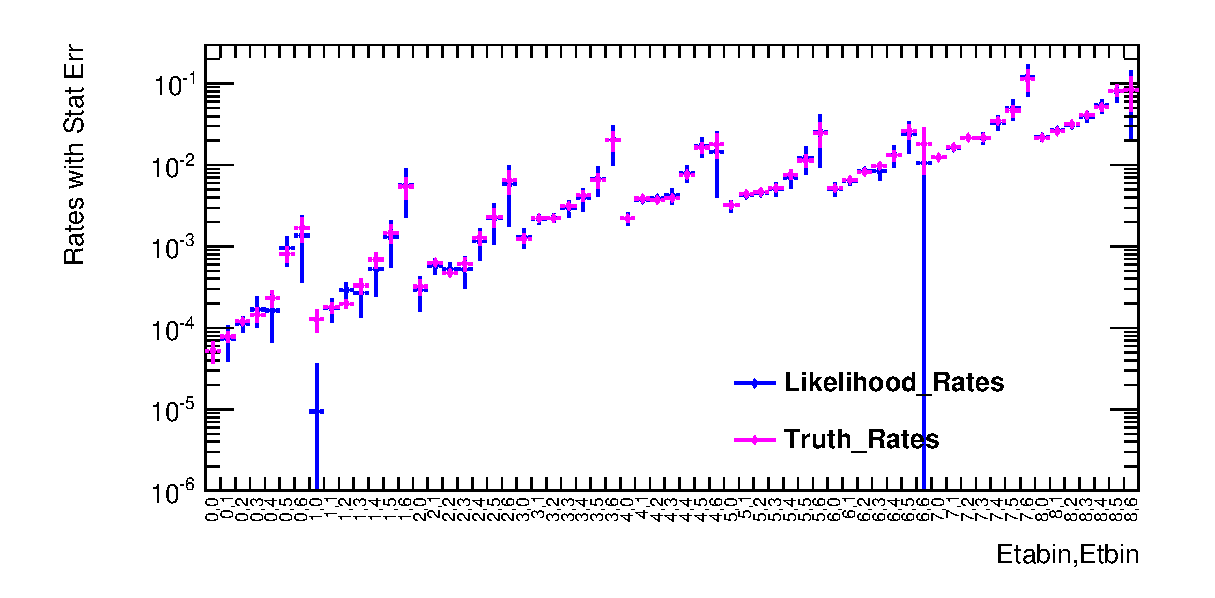
\includegraphics[width=0.8\textwidth]{figures/ChargeMisID/LL_TR_Com.eps}
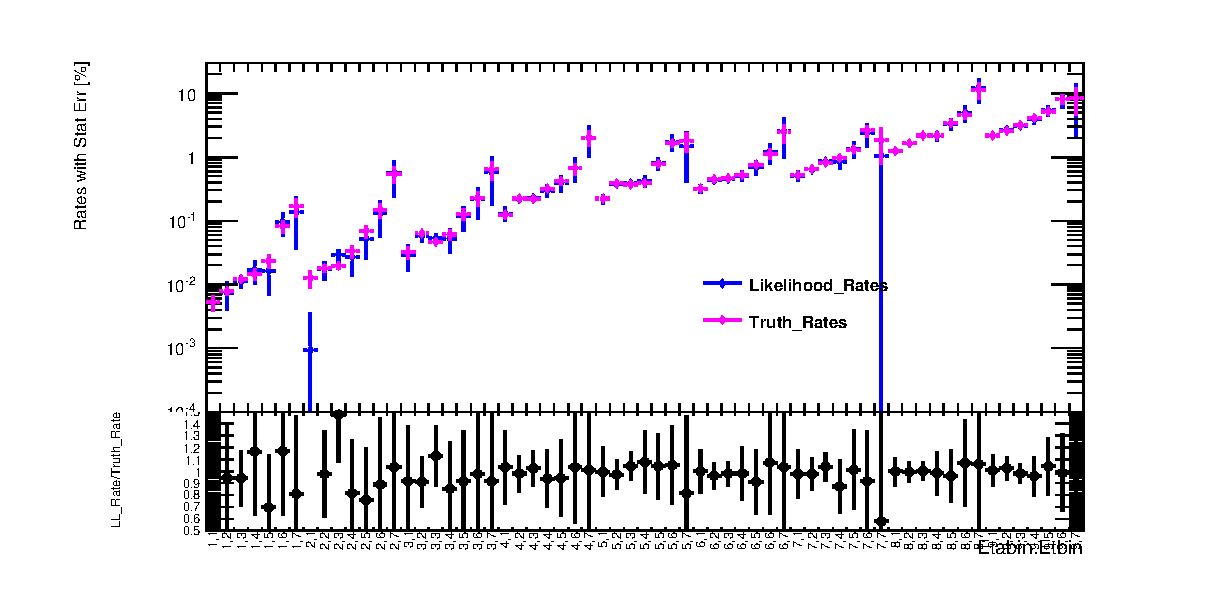
\includegraphics[width=0.8\textwidth]{figures/ChargeMisID/LL_TR_Com_new.eps}

\caption{Comparisons of the charge misID rates obtained with the likelihood method and the truth method. The two sets of rates shown here were both measured with the same \Zee\ MC sample.
Statistical errors are shown. The $x$ axis label is
  the $|\eta|$, \pt\ bin index, as defined in Table~\ref{tab:Etbin and Etabin of mis-charge rate}.}
  
% This is mis-charge rate comparison between likelihood and
%   truth method considering statistic errors. The two sets of rates
%   here are both measured with \Zee\ MC samples. The $x$ axis label is
%   the \eta, \pt\ bin index.}
\label{fig:LL_Truth_Comparison}
\end{figure}  

% Through the comparison, one can see that the rates measured with the
% likelihood method are compatible with that obtained with the truth
% method. The difference between these two sets of rates is taken into account as a systematic in the final measurement.
%

 % \subsubsection{Estimation of the charge misID rates in the data}


The misID rates measured in data using the likelihood method are shown in Figure~\ref{fig:LL_Rates_Egamma}.

% The likelihood method is then applied in the data to measure the charge misID rates.
%  % using the skimmed data from Egamma stream.
% % in Egamma stream we measure the data-driven rates with
% % (\texttt{user.along528.data12\_8TeV.period*.physics\_EGamma.PhysCont.NTUP\_SMWWW.SMN2N\_2\\Lep\_v1\_EXT0}
% % where * is A,B,C,D,E,G,H,I,J,L. These samples are slimmed with loose
% % di-lepton requirement, the di-lepton slim require there are at least 2
% % tagged high \pt\ leptons where tagged high \pt\ means Electron/Muon
% % satisfies any object quality requirement (loose, medium or tight for
% % muons and loose++,\\medium++,tight++,
% % veryLooseLL,looseLL,mediumLL,tightLL, or veryTightLL for electrons)
% % and has a pt of at least 10 GeV.).
%
% They are measured using the same selection described above. This estimation is used as the central value for the charge misID rates measurement. Figure~\ref{fig:LL_Rates_Egamma}, show the central value of the rate and their statistical error as a function of the $|\eta|$ and \pt\ bin index defined in Table~\ref{tab:Etbin and Etabin of mis-charge rate}.

% They are shown as a function of the \eta and \pt\ bin index defined in Table~\ref{tab:Etbin and Etabin of mis-charge rate}, in Figure~\ref{fig:LL_Rates_Egamma}.


\begin{figure}[htp]
\centering
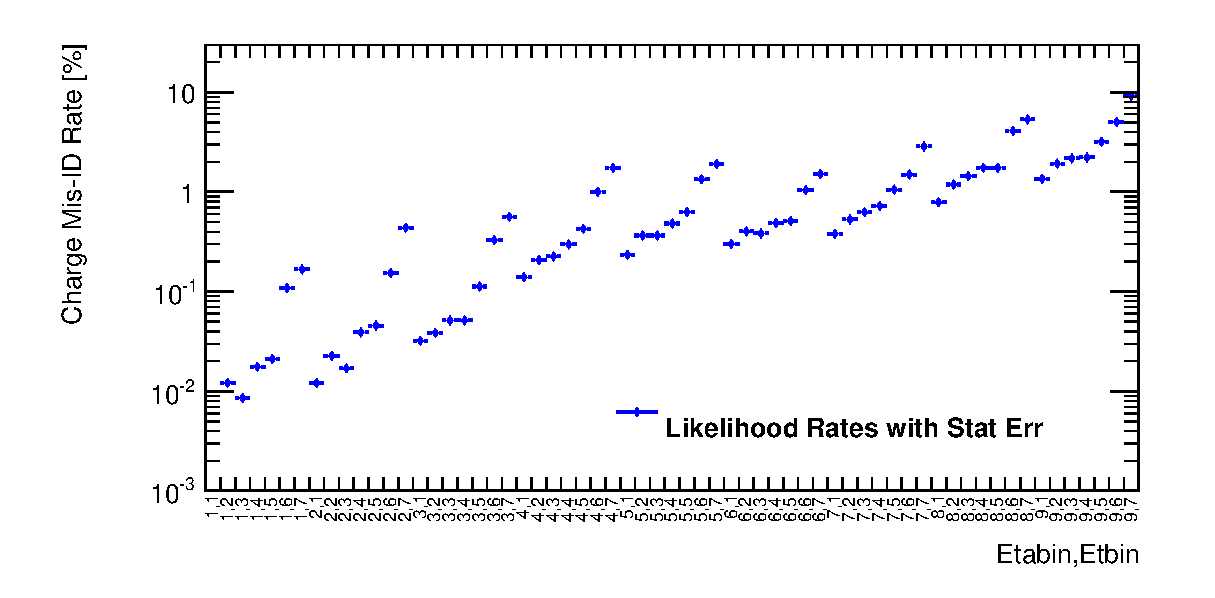
\includegraphics[width=0.8\textwidth]{figures/ChargeMisID/Egamma_LLB_new.eps}
\caption{Electron charge misID rates obtained from data with the likelihood method. Statistical errors are shown. The $x$ axis label is
  the $|\eta|$, \pt\ bin index, as defined in Table~\ref{tab:Etbin and Etabin of mis-charge rate}.}

% This is electron mis-charge rates measured from data with likelihood method and its statistic errors. Label on x axis is \eta, \pt\ bin indices.}
\label{fig:LL_Rates_Egamma}
\end{figure}


 \subsubsection{Systematic effect on charge misID rates due to background contamination}

The contamination of non-$Z\rightarrow{}ee$ processes in the previous selection is taken into account as a systematic.

In order to study this effect, a template fit approach is used. The signal template is obtained from the same MC simulation sample used above, while the background template is obtained from a looser data selection enriched in background events. Due to statistic constraints the background template is obtained in each $|\eta|$ bins, but the $\pt$ bins are grouped together. The event selection for the background template request the presence of a good isolated electron as defined in Section~\ref{sec:Object_selection}, and a second electron failing the tight++ identification cut. 

The two templates are then used on the invariant mass distribution of the electron pairs, in each $\pt$ and $|\eta|$ bins to determine the background contribution, subtract it and recompute the rate by maximizing the likelihood defined in Eq.~(\ref{eq:lnL_chargeMisID}). The difference between this new set of rates and the central value is then taken as a systematic uncertainty on the method, and are summarized in Table~\ref{tab:Charge_MisID_Bkg_Sys}. Further details on this method are also provided in Appendix~\ref{sec:appendix_chargeMisID}.

% The uncertainty due to the background contamination is summarized in Table~\ref{tab:Bkg Sys}.

% We estimate the background effect with
% coarser binning and include the shift in mischarge rate in the
% systematics.


%  We apply the likelihood method and event selection mentioned before
%  to data and we get the data-driven electron mis-charge rates, but
%  the rates are measured from data so there will be background events
%  remaining in the selected events. We use those rates directly
%  measured from data as central values and then subtract the
%  background contribution in the rates, we can calculate another set
%  of likelihood rates using the events without background, we may
%  call those rates clean rates. The difference between central values
%  and clean rates is the background systematic.



\begin{table}
\footnotesize
\centering
\begin{tabular}{c|c|c|c|c|c|c|c|c|c}
  \hline
  \backslashbox{\pt[\GeV]}{$|$\eta$|$} &[0,0.8] &[0.8,1.15] &[1.15,1.60] &[1.60,1.80] &[1.80,2.0] &[2.0,2.20] &[2.20,2.30] &[2.30,2.40] &[2.40,2.50] \\ 
  \hline
  [15,30] &8.85 &5.63 &5.75 &5.85 &5.79 &5.64 &5.64 &5.68 &5.49 \\
  \hline
  [30,40] &5.73 &5.71 &5.83 &5.97 &5.75 &5.78 &5.72 &5.81 &5.59 \\
  \hline
  [40,50] &5.76 &5.69 &5.71 &5.71 &5.65 &5.71 &5.62 &5.71 &5.62 \\
  \hline
  [50,60] &5.74 &5.55 &5.64 &5.53 &5.61 &5.65 &5.41 &5.49 &5.65 \\
  \hline
  [60,80] &5.77 &5.57 &5.71 &5.99 &5.59 &5.66 &5.35 &5.53 &5.41 \\
  \hline
  [80,120] &5.79 &5.63 &5.73 &5.71 &5.74 &5.77 &5.36 &5.74 &5.89 \\
  \hline
  [120,1000] &5.76 &5.71 &5.54 &5.76 &5.52 &5.61 &5.73 &5.98 &6.14  \\
  \hline
\end{tabular}
\caption{Systematic uncertainties on the central value charge misID rates expressed in percent. These uncertainties were obtained considering the impact of the background contamination in the selection.}
% Numbers here are background systematics over central values
%   in percent.}
\label{tab:Charge_MisID_Bkg_Sys}
\end{table} 
 


\subsubsection{Final rates}

The rates with the final errors used in the analysis are shown in Figure~\ref{fig:ChargeMisID_truthRate_finalFig}. The total systematic uncertainty is obtained doing a quadratic sum of the error obtained comparing the MC likelihood method and the truth method, shown in Table~\ref{tab:MCLLTruthSys}, and the error obtained considering the background contamination in the selection. The rates are also given in Table~\ref{tab:LL_finalRates}.

 \begin{figure}[htp]
 \centering
 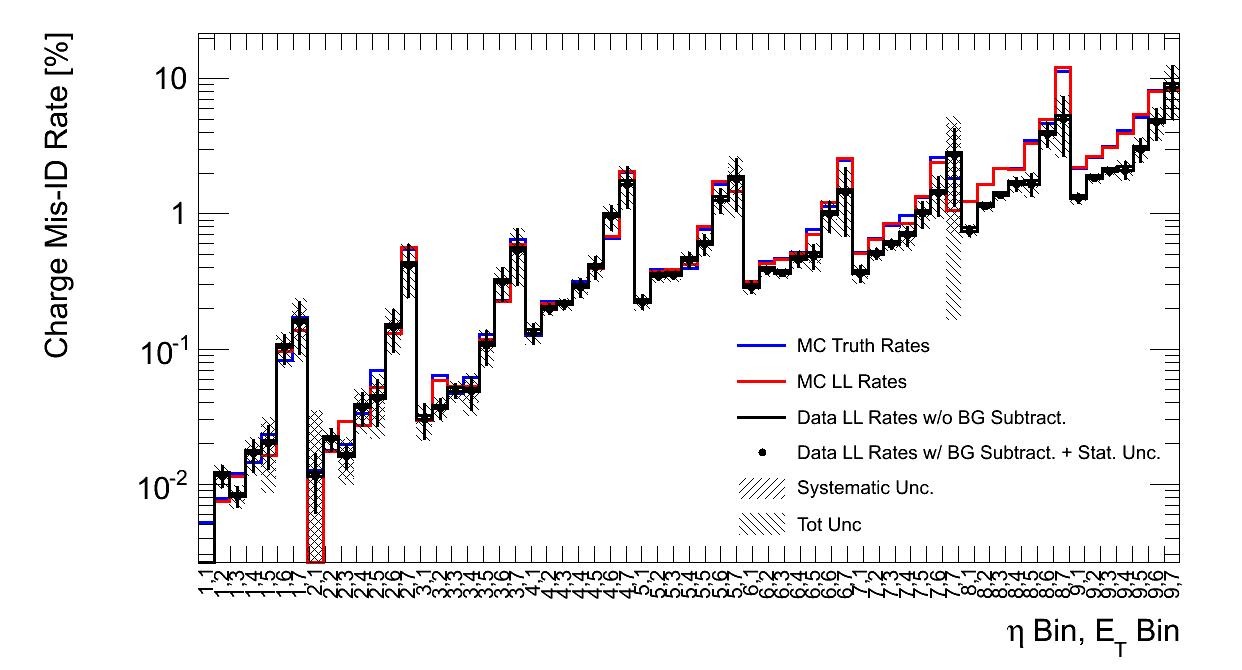
\includegraphics[width=0.8\textwidth]{figures/ChargeMisID/Validation_ChargeMisIDRates_PTvsEta_FinalRateWithSys.png}
 \caption{Electron charge misID rates obtained from data with the likelihood method. All the errors are now shown. The $x$ axis label is
  the $|\eta|$, \pt\ bin index, as defined in Table~\ref{tab:Etbin and Etabin of mis-charge rate}.}
 \label{fig:ChargeMisID_truthRate_finalFig}
 \end{figure}

\begin{table}
\footnotesize
\centering
\begin{tabular}{c|c|c|c|c|c|c|c|c|c}
  \hline
  \backslashbox{\pt[\GeV]}{$|$\eta$|$} &[0,0.8] &[0.8,1.15] &[1.15,1.60] &[1.60,1.80] &[1.80,2.0] &[2.0,2.20] &[2.20,2.30] &[2.30,2.40] &[2.40,2.50] \\
  \hline
  [15,30] & $> 100$ & $> 100$ &9.24 &3.12 &0.70 &0.05 &2.27 &0.25 &0.80 \\
  \hline
  [30,40] & 5.98 &2.58 &9.91 &2.14 &2.97 &3.84 &2.51 &0.63 &2.44\\
  \hline
  [40,50] & 6.22 &32.26 &11.36 &2.19 &4.12 &2.17 &3.52 &0.43 &2.13 \\
  \hline
  [50,60] & 14.22 &22.92 &17.20 &6.72 &7.13 &2.08 &14.80 &1.75 &4.52 \\
  \hline
  [60,80] & 43.45 &32.03 &9.39 &6.14 &3.93 &9.86 &1.19 &4.22 &3.84 \\
  \hline
  [80,120] & 14.59 &12.57 &2.51 &3.14 &4.73 &6.90 &9.40 &6.40 &1.34 \\
  \hline
  [120,1000] & 23.46 &3.02 &9.53 &1.02 &22.98 &3.17 &73.12 &5.61 &3.31 \\
  \hline
\end{tabular}
\caption{The absolute value of the difference between the charge mis-identification rates derived in MC using the truth method and using the likelihood method.  Numbers
are shown as a percent of the MC likelihood method.  These are transported to the likelihood rates in data and used as a systematic. }
\label{tab:MCLLTruthSys}
\end{table}



\begin{table}
\footnotesize
\centering
\begin{tabular}{c|c|c|c|c|c|c|c|c|c}
  \hline
  \backslashbox{\pt[\GeV]}{$|$\eta$|$} &[0,0.8] &[0.8,1.15] &[1.15,1.60] &[1.60,1.80] &[1.80,2.0] &[2.0,2.20] &[2.20,2.30] &[2.30,2.40] &[2.40,2.50] \\
  \hline
  $ \times 10^{}$
  [15,30] &$1.7370\times 10^{-11}$ &$9.4036\times 10^{-6}$ &0.0003 &0.0013 &0.0022 &0.0032 &0.0051 &0.0124 &0.0219\\
  \hline
  [30,40] &$7.4276\times 10^{-5}$ &0.0002 &0.0006 &0.0022 &0.0038 &0.0043 &0.0064 &0.0165 &0.0268 \\
  \hline
  [40,50] &0.0001 &0.0003 &0.0005 &0.0023 &0.0039 &0.0046 &0.0085 &0.0218 &0.0311 \\
  \hline
  [50,60] &0.0002 &0.0003 &0.0005 &0.0030 &0.0042 &0.0051 &0.0085 &0.0213 &0.0394 \\
  \hline
  [60,80] &0.0002 &0.0005 &0.0012 &0.0040 &0.0080 &0.0070 &0.0134 &0.0332 &0.0540 \\
  \hline
  [80,120] &0.0009 &0.0013 &0.0023 &0.0068 &0.0172 &0.0122 &0.0239 &0.0497 &0.0810 \\
  \hline
  [120,1000] &0.0014 &0.0056 &0.0059 &0.0204 &0.0147 &0.0255 &0.0106 &0.1208 &0.0820  \\
  \hline
\end{tabular}
\caption{Electron charge mis-ID rates, obtained with the likelihood method on the data.}
\label{tab:LL_finalRates}
\end{table}




Although the likelihood method, which is used to determined the rates from the data, was validated in MC using the truth method, it is quite important to validate the rates as much as possible, and to verify that if there are remaining differences they are covered within the systematic uncertainties that were assigned.

%As already stated, the charge misID rates are particularely important for the determination of the $WZ$ and $ZZ$ background contamination in the 0SFOS region. Therefore two more tests are conducted to test their validity.

We performed a test to recompute the charge misID rates using the truth method and a $WZ$ MC sample, and compare these new rates to the old one obtained with the $Z\to{}ee$ events. In principle, the charge misID is mostly due to detector effects, and it is therefore not expected to see any differences using one physics process or another one, as long as the GEANT4 geometry of the detector that was used to generate the events is the same. To perform this study, given the lower statistic available in the $WZ$ MC sample a different binning is used, it is summarized in Table~\ref{tab:Etbin and Etabin of mis-charge rate for WZ comparisons}. The new rates obtained are compared in Figure~\ref{fig:ChargeMisID_truthRate_Zee_WZ}. In this figure only the statistical error of each measurement is shown. A very good agreement between the two sets of rates is observed.



\begin{table}[htp]
\centering

\begin{tabular}{c|c||c|c}
	 \hline
	  $|\eta|$ bins & $|\eta|$ bin index   & \pt\ bins [\GeV] & \pt\ bin index \\
 	 \hline
	  $[0, 1.15]   $   & 0 	   &  $[15, 40]$ & 0 \\
	  $[1.15, 1.8] $   & 1 	   &  $[40, 60]$ & 1 \\
	  $[1.8, 2.2] $   & 2	   &  $[60, 100]$ & 2 \\
	  $[2.2, 2.5] $   & 3 	   &  $[100, 1000]$ & 3 \\

  \hline
\end{tabular}
\caption{The $|\eta|$ and \pt\ bins used for the comparison of mischarge
  rate obtained with MC $Z\to{}ee$ sample and MC $WZ$ sample. The bin index used in the 1D figures~\ref{fig:ChargeMisID_truthRate_Zee_WZ} are given.}
\label{tab:Etbin and Etabin of mis-charge rate for WZ comparisons}
\end{table}



 \begin{figure}[htp]
 \centering
 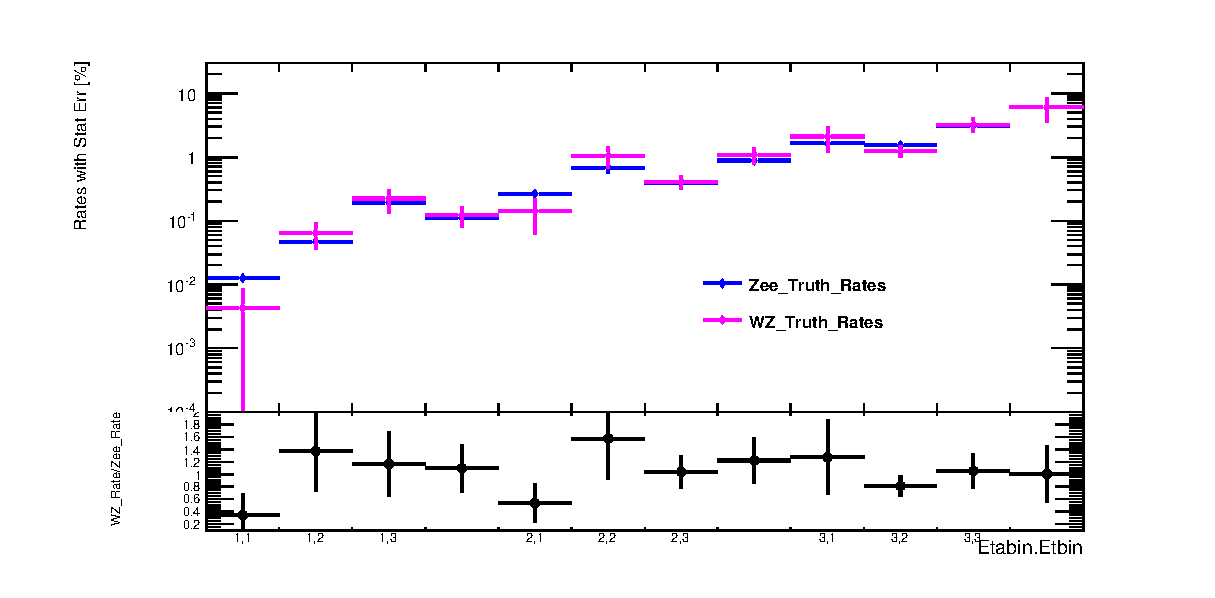
\includegraphics[width=0.8\textwidth]{figures/ChargeMisID/Validation_ChargeMisIDRates_PTvsEta_CompareSSRate.eps}
 \caption{Electron charge misID rates obtained from MC $Z\to{}ee$ with the likelihood method are compared with rates obtained using the truth method in a MC $WZ$ sample. Errors shown here are purely statistics. The $x$ axis label is
  the $|\eta|$, \pt\ bin index, as defined in Table~\ref{tab:Etbin and Etabin of mis-charge rate for WZ comparisons}.}
 \label{fig:ChargeMisID_truthRate_Zee_WZ}
 \end{figure}


\subsubsection{Application and validation of rates}
As already stated, the charge misID rates are primarily important for the determination of the $WZ$ and $ZZ$ background contamination in the 0SFOS region. 
Once derived, the rates are applied to $WZ$ and $ZZ$ MC samples based on whether or not a charge flip could cause the event to appear in the 0 SFOS region.  
In particular, the following di-boson decays are considered:
\begin{itemize}
\item $WZ\rightarrow e^{\pm}\nu~ e^{+}e^{-}$
\item $WZ\rightarrow \mu^{\pm}\nu~ e^{+}e^{-}$
\item $WZ\rightarrow \tau^{\pm}\nu~ e^{+}e^{-}$
\item $ZZ\rightarrow e^{+}e^{-}~e^{+}e^{-}$
\item $ZZ\rightarrow \mu^{+}\mu^{-}~ e^{+}e^{-}$
\end{itemize}
No other decay channels are considered.  These all share in common that they have at least one electron-positron pair.  
Except for the $WZ\rightarrow \tau^{\pm}\nu~e^{+}e^{-}$ decay channel, decay channels with tau leptons are not considered
because they are suppressed by the tau branching fraction and are considered to be negligible.

The charge mis-identification rates are then applied to these channels on an event-by-event basis as follows.
For each event that is processed, its decay channel is identified at truth level. Each reconstructed lepton
is examined  and assigned a rate, or a probability to charge flip, based on its reconstructed $\pt$ and $\eta$ values.
The probability for a charge flip to occur in an event is then approximately the sum of rates for the individual electrons:
\begin{equation}
\textrm{Probability of Charge Mis-Identification in Event} = \sum_{i \in \textrm{Electrons}}  \textrm{Rate}(\pt^i,\eta^i) + \textrm{Higher Order Terms}
\end{equation}
Higher order terms where multiple electrons are charge mis-identified is small and considered to be negligible.
We are only concerned with the probability that a charge flip results in the event falling into the 0 SFOS region. 
Consider a step function, $\Theta(e)$, defined for an individual event:
\[
\Theta(e) = 
\begin{cases}
\hfill 1 \hfill & \text{if flipping charge of $e$ classifies event as 0 SFOS} \\
\hfill 0 \hfill & \text{if flipping charge of $e$ does NOT classify event as 0 SFOS}\\
\end{cases}
\]
Then the probability that a charge mis-identification occurs and results in the event falling in the 0 SFOS region is:
\begin{equation}
\textrm{Probability that event is classified as 0 SFOS} = \sum_{i \in \textrm{Electrons}}  \textrm{Rate}(\pt^i,\eta^i)\Theta(i) + \textrm{Higher Order Terms}
\end{equation}
Again, we ignore the case where multiple electrons have their charge mis-identified.  
This probability is then used as an event by event weight. 



Once the weight has been determined, we then artificially flip the charge of one of the electrons/positrons in the event.
If there is only one electron in the event that will lead the event to fall in the 0 SFOS region, its charge is flipped
and one proceeds to the next event.  However, if there are multiple electrons in the event, there is an ambiguity that must be resolved
about which electron's charge should be flipped. One must then be careful in this case to not introduce any bias.
We decided to choose a procedure where we pick a single electron from the event at random based on the charge flip rates
of the individual electrons. Thus, for an individual electron in an event, the probability that it is chosen to have its charge
flipped is:
\begin{equation}
\textrm{Probability that $e$ has charge flipped} = \textrm{Rate}(\pt^e,\eta^e)\Theta(e)~/\sum_{i \in \textrm{Electrons}} \textrm{Rate}(\pt^i,\eta^i)\Theta(i)
\end{equation}

Consider an example 
where the event under consideration comes from the decay $WZ\rightarrow e^{+}\nu e^{+}e^{-}$. Assume all three charged leptons pass reconstruction and are selected then label them as: $e^{+}_1~e^{+}_2e^{-}_3$. In this case,
the only way that this event could be classified as 0 SFOS when flipping the charge of only one electron/positron is to flip the charge of the electron.
Thus, $\Theta(e^{+}_1)=\Theta(e^{+}_2)=0$ and $\Theta(e^{-}_3)=1$.  The event weight will then be equal to the rate of charge mis-identification for  $e^{-}_3$ and it
will have it's charge flipped to be positive.

Now consider an example of an event with the decay of $ZZ\rightarrow \mu^{+}\mu^{-}~ e^{+}e^{-}$.
If all four leptons are reconstructed and selected, the event will not be considered at all in the three lepton selection of this analysis, so consider the 
case where the $\mu^{+}$ is not selected leaving three leptons labeled as: $\mu^{-}_1 e^{+}_2 e^{-}_3$.  The probability for the muon to charge flip
is negligible which leaves the electron and the positron. Flipping the charge of either one at a time will result in the event being classified as 0 SFOS.  Thus, in
this case $\Theta(\mu^{-}_1)=0$ and $\Theta(e^{+}_2)=\Theta(e^{-}_3)=1$. The event weight will then be the sum of the rates for $e^{+}_2$ and $e^{-}_3$.
The probability that the electron has its charge flipped is then $\frac{\textrm{Rate}(e^{-}_3) }{ \textrm{Rate}(e^{+}_2)+ \textrm{Rate}(e^{-}_3)}$ and similarly for the positron.

This procedure has been validated on the $WZ$ and $ZZ$ samples by comparing the predictions taken directly from MC to the predictions reweighted in the 0 SFOS signal region using the procedure just described. This is done in Figure~\ref{fig:ChargeMisID_Validation_WZ} for the $WZ$ samples and on Figure~\ref{fig:ChargeMisID_Validation_ZZ} for the $ZZ$ samples. It can be seen the agreement in the shape looks good for all the distributions. An offset between the two distributions is observed. This difference is covered partially by the systematic uncertainties of the method.  Any remaining difference could be expected from the difference in rates observed at high $\eta$ and high $E_{T}$ as seen in Fig.~\ref{fig:ChargeMisID_truthRate_finalFig} and serves as justification for using the data-driven method.

There is no special treamtent of the charge mis-identification contribution to other background contributions in the 0 SFOS region or to any contributions to the 
1 and 2 SFOS signal regions, including diboson processes, as the effect is expected to be very small.  Any charge mis-identification events are thus taken directly 
from MC in this case.


 \begin{figure}[htp]
 \centering
 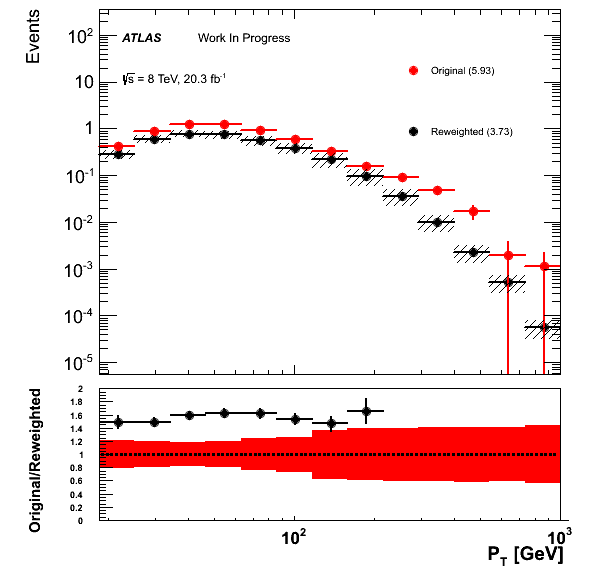
\includegraphics[width=0.4\textwidth]{figures/ChargeMisID/Validation_ChargeMisIDRates_WZ_PTLepton.png}
 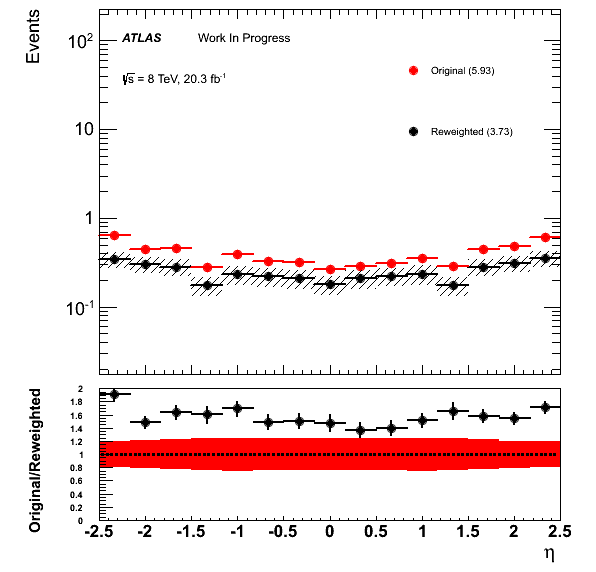
\includegraphics[width=0.4\textwidth]{figures/ChargeMisID/Validation_ChargeMisIDRates_WZ_EtaLepton.png}
 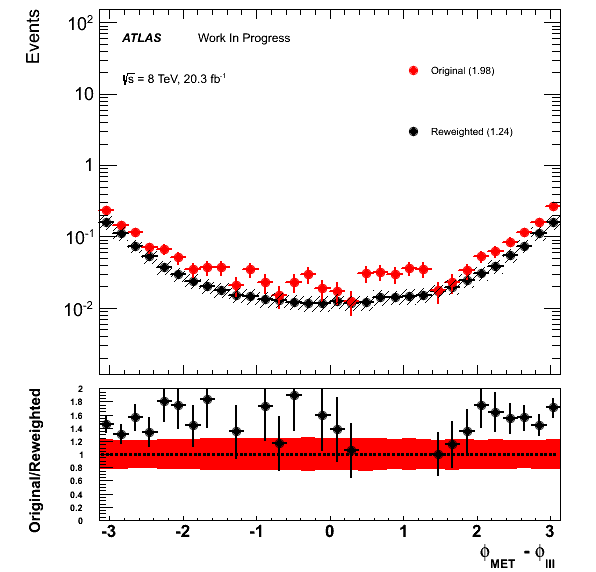
\includegraphics[width=0.4\textwidth]{figures/ChargeMisID/Validation_ChargeMisIDRates_WZ_DeltaPhi.png}
 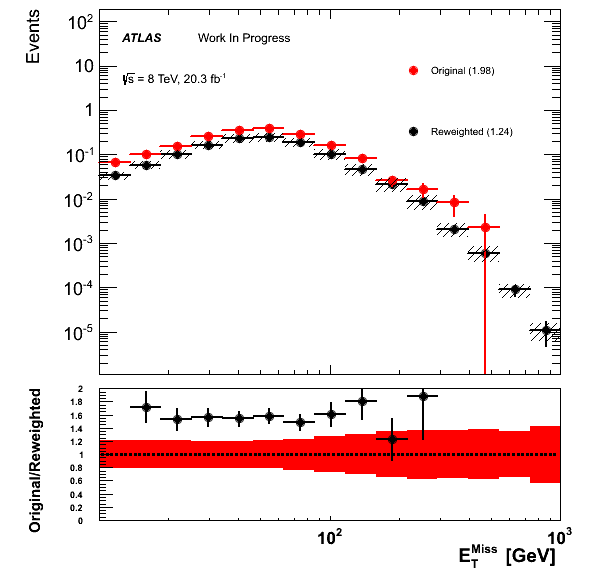
\includegraphics[width=0.4\textwidth]{figures/ChargeMisID/Validation_ChargeMisIDRates_WZ_MET.png}
 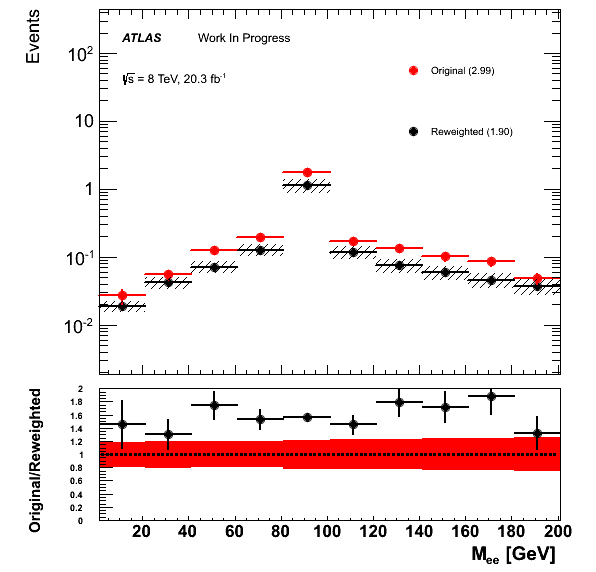
\includegraphics[width=0.4\textwidth]{figures/ChargeMisID/Validation_ChargeMisIDRates_WZ_Mee.png}
 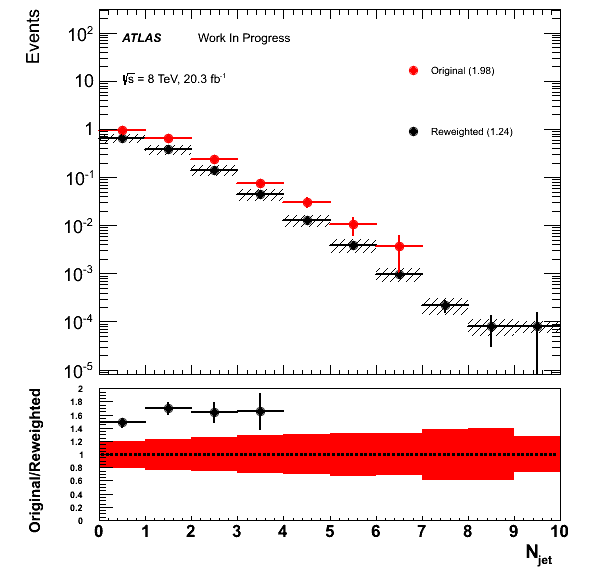
\includegraphics[width=0.4\textwidth]{figures/ChargeMisID/Validation_ChargeMisIDRates_WZ_JetMultiplicity.png}

 \caption{Validation of the charge mis-ID rates comparing MC $WZ\rightarrow \ell ee$ ($\ell=e,\mu$) samples reweighted with the charge misID rates measured in the MC $Z\to{}ee$ 
 sample to the original MC predictions. Distribution of lepton $p_{T}$, $\eta$, $\Delta \phi(3l,E_{T}^{Miss})$,\met{}, Same-sign di-electron invariant mass, and jet multiplicity.}
 \label{fig:ChargeMisID_Validation_WZ}
 \end{figure}
 
 
 \begin{figure}[htp]
 \centering
 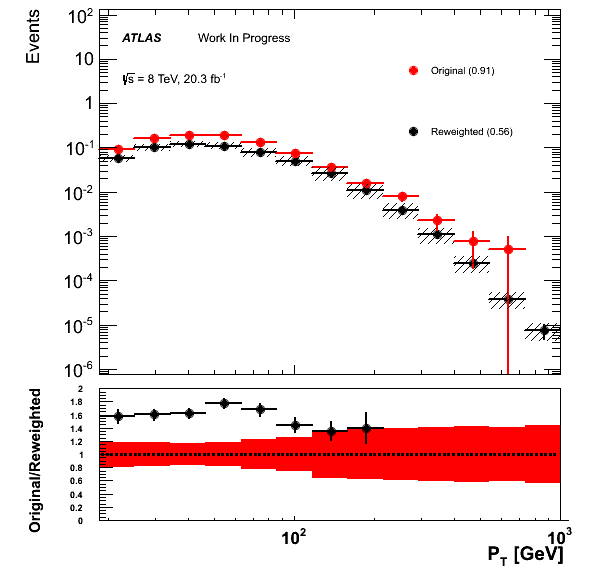
\includegraphics[width=0.4\textwidth]{figures/ChargeMisID/Validation_ChargeMisIDRates_ZZ_PTLepton.png}
 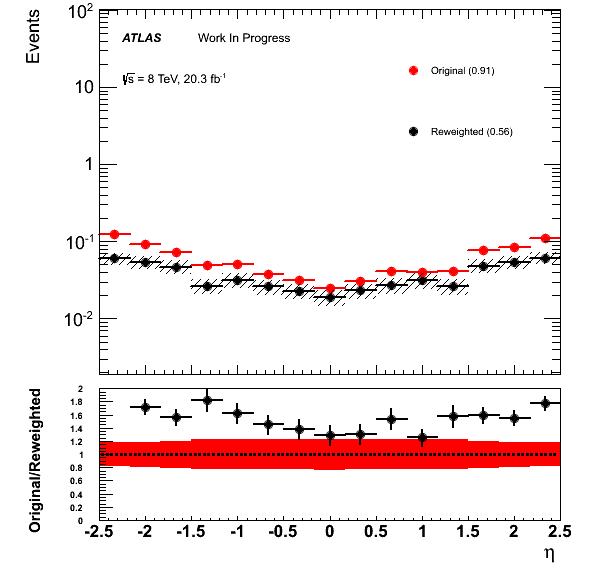
\includegraphics[width=0.4\textwidth]{figures/ChargeMisID/Validation_ChargeMisIDRates_ZZ_EtaLepton.png}
 \includegraphics[width=0.4\textwidth]{figures/ChargeMisID/Validation_ChargeMisIDRates_ZZ_DeltaPhi.png}
 \includegraphics[width=0.4\textwidth]{figures/ChargeMisID/Validation_ChargeMisIDRates_ZZ_MET.png}
 \includegraphics[width=0.4\textwidth]{figures/ChargeMisID/Validation_ChargeMisIDRates_ZZ_Mee.png}
 \includegraphics[width=0.4\textwidth]{figures/ChargeMisID/Validation_ChargeMisIDRates_ZZ_JetMultiplicity.png}

 \caption{Validation of the charge mis-ID rates comparing MC $ZZ\rightarrow \ell \ell ee$ ($\ell=e,\mu$) samples reweighted with the charge misID rates measured in the MC $Z\to{}ee$ 
 sample to the original MC predictions. Distribution of lepton $p_{T}$, $\eta$, $\Delta \phi(3l,E_{T}^{Miss})$,\met{}, Same-sign di-electron invariant mass, and jet multiplicity.}
 \label{fig:ChargeMisID_Validation_ZZ}
 \end{figure}







\subsubsection{Background samples}
\label{sec:www_bg}

There are other processes produced in proton-proton collisions at the LHC
which can mimic the signal processes. These are referred to as background processes.
In many cases, the background processes are either
more abundant than or of a similar abundance to
the signal. As a result, they must be well understood if there is any hope
of distinguishing between the two. The background processes to the signal
are characterized by having either at least three prompt leptons, meaning they
come directly from the hard scattering process;  
two prompt leptons and an isolated photon, which can mimic an electron;
or two prompt leptons and a jet that mimics a lepton.
The first two are estimated primarily using MC simulation while the third type
is estimated using the data itself. 
This will be described in more detail in \sec\ref{sec:bg_fake}.
For now, we will focus only on the processes estimated using MC simulation.

The most important backgrounds are those with at least three prompt leptons, 
hereby referred to as the prompt backgrounds. Of these prompt backgrounds,
the $WZ$ process is the most important since it has a 
large cross-section (compared to the signal)
and results in a final state with exactly three leptons. Another important 
prompt background is the $ZZ$ process,
which has a similar cross-section to the $WZ$ process, but is typically 
selected by producing
four leptons and then not measuring one. Thus, this process is supressed by the 
efficiency for not measuring the presence of a lepton. 
These are collectively referred to as the di-boson processes, sometimes
indicated as $VV$ where $V=W/Z$ (the $WW$ process is also considered
but can only produce at most two prompt leptons making it negligible). 
The di-boson processes are produced using the 
the \powheg~\cite{Alioli:2008gx,Nason:2004rx,Frixione:2007vw,Alioli:2010xd} generator
with the CT10 NLO PDF set and 
hadronized through \pythiaeight~using the AU2 tune, same as the signal.

Other prompt backgrounds 
inlcude tri-boson processes like $ZWW$ and $ZZZ$ 
(typically referred to collectively as $VVV$)
and \ttV~production. Tri-boson processes
have cross-sections of a similar size to the signal but are supressed 
for a similar reason
as the $ZZ$, since these can produce either four or six lepton final 
states. 
\ttV~production is when a vector
boson is produced in conjuction with a \tt~pair. 
Since the top quark almost always decays
into a $W$-boson and a $b$-quark, \ttV~production also results in an intermediate
state of three vector bosons which ultimately results in a three to four lepton
final state.
The $VVV$ and \ttV~processes were generated using \madgraph with the 
CTEQ6L1 PDF set and hadronized
using \pythiasix~\cite{PYTHIA} with the AUET2B~\cite{ATL-PHYS-PUB-2011-009} 
tune.

The second category of backgrounds to consider are those with two 
prompt leptons and a photon. We will call these the photon backgrounds.
This background occurs entirely from the di-boson process $Z\gamma$
where the $Z$ boson decays to two leptons and the photon mimics an electron.
A photon is measured
by observing an energy deposit in the electromagnetic calorimeter 
without any associated track in the inner detector.
A photon can mimic an electron
if it converts into an electron-positron
pair while still inside the inner detector, thereby leaving a track 
in the inner detector while still leaving an energy deposit in the 
calorimeter, the tell-tale sign of an electron.
The $Z\gamma$ samples were generated with the \sherpa~\cite{sherpa} generator 
and the CT10 PDF set.  %hadronization? CT10 NLO? Or LO?
In addition to this process, the $W\gamma$ process behaves similarly 
but only has one prompt lepton in addition to the photon, so it is negligible.
Still, we generate it by using
the \alpgen~\cite{ALPGEN} generator with the CTEQ6L1 PDF set
and hadronize it using \jimmy~\cite{Jimmy} with the AUET2C~\cite{ATL-PHYS-PUB-2011-009} 
tune.

Some of the di-boson and tri-boson processes just discussed can also be produced
through loop induced processes or double parton scattering.
The $WW$ and $ZZ$
loop induced processes are generated using the gg2ZZ~\cite{Binoth:2008pr} 
and gg2WW~\cite{Binoth:2006mf} generators with the CT10 PDF set and
hadronized using JIMMY with the AU2 tunes.
The double parton scattering
processes are generated using \pythiaeight with the AU2 
tunes and the CTEQ6L1 PDF set. 

The last category of backgrounds are those with prompt leptons plus
jets that mimic leptons. These are nominally estimated using the data
as decribed in \sec\ref{sec:bg_fake}. However, some of the contributions
to this background can be simulated using MC as a cross-check of 
the estimate from data and for other studies. The main contributions
to this are the single boson processes ($V+$jets) and \tt~production.
These are processes with very large cross-sections so
that even though the probability for a jet mimicking a lepton is small,
the size of the cross-section means that their contribution is non-negligible.
The single boson process of $Z+$jets are generated using \sherpa~ with the CT10
PDF set while the $W+$jets processes are generated using \alpgen~ with
the CTEQ6L1 PDF set and hadronized using \jimmy~with the AUET2C tunes.
For the $Z+$jets samples, special care must be taken to remove any overlap 
between with the $Z\gamma$ simulated samples described earlier.
Meanwhile, the \tt~processes are generated using the \mcatnlo~\cite{MCatNLO}
generator with the CT10 PDF set and hadronized in JIMMY.  %what is the tune?
Finally, this background also has contributions from single top production,
though it is less important. Single top production is simulated separately 
for the s-channel, t-channel, and $Wt$-channel. The s-channel 
and $Wt$-channel are generated using \mcatnlo~with the CT10 PDF set and 
hadronized through \jimmy~ while the t-channel is generated using \madgraph~
with the CTEQ6L1 PDF set and hadronized using \pythiasix~with the AUET2B tunes.


\section{Corrections and Systematic Uncertainties}
\label{sec:systematics}

The predictions for the signal and background are subject
to the choices made in building the model described thus
far in \sec\ref{sec:www}. If we are to believe our predictions
we must understand how sensitive the predictions are to these choices.
To that end, we also compute the prediction for numerous variations
on the nominal prediction. 
Each one of these variations is called a systematic uncertainty. 
Each systematic uncertainty is designed to assess the sensitivity
to a given choice made when building the model. 
This analysis has almost 50 different systematic
uncertainties, each of which is varied independently. The size of 
each systematic uncertainty
is treated as a separate nuisance parameter
as input to the statistical model used in the interpretation of the model
when compared to data, described later in \sec\ref{sec:measurement}.

The systematic uncertainties can be split up into four categories:
theory, methodology, experiment, and luminosity. 
I will summarize them below, in each case giving the 
size of the uncertainties in the three signal regions. 
Some of these variations have 
been mentioned already in previous sections but will be
referred to here again for completeness.

\subsection{Theoretical Uncertainties}




\begin{table}[ht]
\centering
\small\renewcommand{\tabcolsep}{4pt}
\begin{tabular}{|cl||ccccccc|c||c|}
\hline
 & & \multicolumn{8}{c||}{Background} & Signal \\ 
 & & $WZ$ & $ZZ$ & $VVV$ & $t\overline{t}+V$ & DPS & $Z\gamma$ & Fake & Total & \\ 
 & & &  &  &  &  &  & (Data) & BG & \\ 
\hline\hline
\multirow{2}{*}{Signal}
&PDF & --- & --- & --- & --- & --- & --- & --- & --- &  $2.80$ \\ 
\cline{2-11}
& $\mu_{R}$ and $\mu_{F}$ Choice &  --- &  --- &  --- &  --- &  --- &  --- &  --- &  --- & $2.60$\\ 
\hline
\multirow{5}{*}{Norm.}
& $WZ$ & $10.00$&  --- &  --- &  --- &  --- &  --- &  --- & $2.63$&  ---\\ 
\cline{2-11}
& $ZZ$ &  --- & $15.00$&  --- &  --- &  --- &  --- &  --- & $0.42$&  ---\\ 
\cline{2-11}
& $VVV$ &  --- &  --- & $30.00$&  --- &  --- &  --- &  --- & $1.44$&  ---\\ 
\cline{2-11}
& $t\overline{t}+V$ &  --- &  --- &  --- & $30.00$&  --- &  --- &  --- & $0.50$&  ---\\ 
\cline{2-11}
& DPS &  --- &  --- &  --- &  --- & $50.00$&  --- &  --- &  --- &  ---\\ 
\hline
\end{tabular}

\caption{Size of theoretical uncertainties in percent for the 0 SFOS signal region. The background uncertainties are shown for the individual background components as well as the total. The signal uncertainty is shown separately. Those marked --- are either not applicable or below 0.02 \% and thus considered to be negligible}
\label{tab:sys_theory_0sfos}
\end{table}

\begin{table}[ht]
\centering
\small\renewcommand{\tabcolsep}{4pt}
\begin{tabular}{|cl||ccccccc|c||c|}
\hline
 & & \multicolumn{8}{c||}{Background} & Signal \\ 
 & & $WZ$ & $ZZ$ & $VVV$ & $t\overline{t}+V$ & DPS & $Z\gamma$ & Fake & Total & \\ 
 & & &  &  &  &  &  & (Data) & BG & \\ 
\hline\hline
\multirow{2}{*}{Signal}
& PDF &  --- &  --- &  --- &  --- &  --- &  --- &  --- &  --- & $2.80$\\ 
\cline{2-11}
& $\mu_{R}$ and $\mu_{F}$ Choice &  --- &  --- &  --- &  --- &  --- &  --- &  --- &  --- & $2.60$\\ 
\hline
\multirow{5}{*}{Norm.}
& $WZ$ & $10.00$&  --- &  --- &  --- &  --- &  --- &  --- & $8.05$&  ---\\ 
\cline{2-11}
& $ZZ$ &  --- & $15.00$&  --- &  --- &  --- &  --- &  --- & $0.59$&  ---\\ 
\cline{2-11}
& $VVV$ &  --- &  --- & $30.00$&  --- &  --- &  --- &  --- & $0.28$&  ---\\ 
\cline{2-11}
& $t\overline{t}+V$ &  --- &  --- &  --- & $30.00$&  --- &  --- &  --- & $0.10$&  ---\\ 
\cline{2-11}
& DPS &  --- &  --- &  --- &  --- & $50.00$&  --- &  --- &  --- &  ---\\ 
\hline
\end{tabular}

\caption{Size of theoretical uncertainties in percent for the 1 SFOS signal region. The background uncertainties are shown for the individual background components as well as the total. The signal uncertainty is shown separately. Those marked --- are either not applicable or below 0.02 \% and thus considered to be negligible}
\label{tab:sys_theory_1sfos}
\end{table}

\begin{table}[ht]
\centering
\small\renewcommand{\tabcolsep}{4pt}
\begin{tabular}{|cl||ccccccc|c||c|}
\hline
 & & \multicolumn{8}{c||}{Background} & Signal \\ 
 & & $WZ$ & $ZZ$ & $VVV$ & $t\overline{t}+V$ & DPS & $Z\gamma$ & Fake & Total & \\ 
 & & &  &  &  &  &  & (Data) & BG & \\ 
\hline\hline
\multirow{2}{*}{Signal}
& PDF &  --- &  --- &  --- &  --- &  --- &  --- &  --- &  --- & $2.80$\\ 
\cline{2-11}
& $\mu_{R}$ and $\mu_{F}$ Choice &  --- &  --- &  --- &  --- &  --- &  --- &  --- &  --- & $2.60$\\ 
\hline
\multirow{5}{*}{Norm.}
& $WZ$ & $10.00$&  --- &  --- &  --- &  --- &  --- &  --- & $8.83$&  ---\\ 
\cline{2-11}
& $ZZ$ &  --- & $15.00$&  --- &  --- &  --- &  --- &  --- & $0.70$&  ---\\ 
\cline{2-11}
& $VVV$ &  --- &  --- & $30.00$&  --- &  --- &  --- &  --- & $0.23$&  ---\\ 
\cline{2-11}
& $t\overline{t}+V$ &  --- &  --- &  --- & $30.00$&  --- &  --- &  --- & $0.07$&  ---\\ 
\cline{2-11}
& DPS &  --- &  --- &  --- &  --- & $50.00$&  --- &  --- & $0.11$&  ---\\ 
\hline
\end{tabular}

\caption{Size of theoretical uncertainties in percent for the 2 SFOS signal region. The background uncertainties are shown for the individual background components as well as the total. The signal uncertainty is shown separately. Those marked --- are either not applicable or below 0.02 \% and thus considered to be negligible}
\label{tab:sys_theory_2sfos}
\end{table}

The theoretical uncertainties are those on the signal PDF and 
on the background cross-section predictions.
They are summarized for the 0, 1, and 2 SFOS regions
in \tab\ref{tab:sys_theory_0sfos}, 
\tab\ref{tab:sys_theory_1sfos}, and
\tab\ref{tab:sys_theory_2sfos}, respectively.
The motivation for the PDF uncertainties has been described
already in \sec\ref{sec:pdf}. 
There are several uncertainties evaluated on the signal PDF, all of which
are described in more detail in \sec\ref{sec:signal}. These
are the PDF choice, including uncertainties reported by the individual
PDFs, as well as variations in the renormalization and factorization scales.
The effect on the signal prediction from these is around 2-3\%.

The most important MC backgrounds have uncertainties evaluated on their
cross-section.  In particular, these are the uncertainties on the 
normalization of the $WZ$, $ZZ$, $Z\gamma$, $VVV$, $\ttV$, 
and DPS background predictions
described in \sec\ref{sec:bg_estimates} and summarized in \tab\ref{tab:mcnorm}.
Their impact when propagated to the final background prediction
varies by channel. In general, the uncertainty on the $WZ$ prediction is the 
largest, contributing about 2.6\% in the 0 SFOS region and around 8-9\%
in the 1 and 2 SFOS regions.  In the 0 SFOS region, the uncertainty 
on the $VVV$ prediction contributes about 1.4\% and that on the $ZZ$ prediction
is about 0.4\%; all others fall below that. 
In the 1 and 2 SFOS regions the $ZZ$ uncertainty is around 0.6-0.7\%; the
rest are negligible. 

\subsection{Methodological Uncertainties}

\begin{table}[ht!]
\centering
\small\renewcommand{\tabcolsep}{4pt}
\begin{tabular}{|cl||ccccccc|c||c|}
\hline
 & & \multicolumn{8}{c||}{Background} & Signal\\ 
 & & $WZ$ & $ZZ$ & $VVV$ & $t\overline{t}+V$ & DPS & $Z\gamma$ & Fake & Total & \\ 
 & & &  &  &  &  &  & (Data) & BG & \\ 
\hline\hline
\multirow{2}{*}{Matrix}
& Electron &  --- &  --- &  --- &  --- &  --- &  --- & $9.62$& $6.20$&  ---\\ 
\cline{2-11}
\multirow{2}{*}{Method}
& Muon &  --- &  --- &  --- &  --- &  --- &  --- & $5.06$& $3.26$&  ---\\ 
\cline{2-11}
& b-jet selection &  --- &  --- &  --- &  --- &  --- &  --- & $90.19$& $58.14$&  ---\\ 
\hline
& Charge Mis-ID & $1.58$& $1.31$&  --- &  --- &  --- &  --- &  --- & $0.45$&  ---\\ 
\hline
\end{tabular}

\caption{Size of the methodological uncertainties in percent for the 0 SFOS signal region. The background uncertainties are shown for the individual background components as well as the total. The signal uncertainty is shown separately. Those marked --- are either not applicable or below 0.02 \% and thus considered to be negligible}
\label{tab:sys_meth_0sfos}
\end{table}

\begin{table}[ht!]
\centering
\small\renewcommand{\tabcolsep}{4pt}
\begin{tabular}{|cl||ccccccc|c||c|}
\hline
 & & \multicolumn{8}{c||}{Background} & Signal\\ 
 & & $WZ$ & $ZZ$ & $VVV$ & $t\overline{t}+V$ & DPS & $Z\gamma$ & Fake & Total & \\ 
 & & &  &  &  &  &  & (Data) & BG & \\ 
\hline\hline
\multirow{2}{*}{Matrix}
& Electron &  --- &  --- &  --- &  --- &  --- &  --- & $36.50$& $4.69$&  ---\\ 
\cline{2-11}
\multirow{2}{*}{Method}
& Muon &  --- &  --- &  --- &  --- &  --- &  --- & $5.11$& $0.66$&  ---\\ 
\cline{2-11}
& b-jet selection &  --- &  --- &  --- &  --- &  --- &  --- & $91.16$& $11.72$&  ---\\ 
\hline
&Charge Mis-ID & --- & --- & --- & --- & --- & --- & --- & --- & ---\\ 
\hline
\end{tabular}

\caption{Size of the methodological uncertainties in percent for the 1 SFOS signal region. The background uncertainties are shown for the individual background components as well as the total. The signal uncertainty is shown separately. Those marked --- are either not applicable or below 0.02 \% and thus considered to be negligible}
\label{tab:sys_meth_1sfos}
\end{table}

\begin{table}[ht!]
\centering
\small\renewcommand{\tabcolsep}{4pt}
\begin{tabular}{|cl||ccccccc|c||c|}
\hline
 & & \multicolumn{8}{c||}{Background} & Signal \\ 
 & & $WZ$ & $ZZ$ & $VVV$ & $t\overline{t}+V$ & DPS & $Z\gamma$ & Fake & Total & \\ 
 & & &  &  &  &  &  & (Data) & BG & \\ 
\hline\hline
\multirow{2}{*}{Matrix}
& Electron &  --- &  --- &  --- &  --- &  --- &  --- & $22.21$& $1.07$&  ---\\ 
\cline{2-11}
\multirow{2}{*}{Method}
& Muon &  --- &  --- &  --- &  --- &  --- &  --- & $6.80$& $0.33$&  ---\\ 
\cline{2-11}
& b-jet selection &  --- &  --- &  --- &  --- &  --- &  --- & $87.19$& $4.20$&  ---\\ 
\hline
&Charge Mis-ID & --- & --- & --- & --- & --- & --- & --- & --- & ---\\ 
\hline
\end{tabular}

\caption{Size of the methodological uncertainties in percent for the 2 SFOS signal region. The background uncertainties are shown for the individual background components as well as the total. The signal uncertainty is shown separately. Those marked --- are either not applicable or below 0.02 \% and thus considered to be negligible}
\label{tab:sys_meth_2sfos}
\end{table}

The methodological uncertainties are those due to the data-driven
modeling of the fake and charge mis-identification backgrounds,
described in \sec\ref{sec:bg_fake} and \sec\ref{sec:charge_misid},
respectively.
They are summarized for the 0, 1, and 2 SFOS regions
in \tab\ref{tab:sys_meth_0sfos}, 
\tab\ref{tab:sys_meth_1sfos}, and
\tab\ref{tab:sys_meth_2sfos}, respectively.
The uncertainty on the fake background is the most important
systematic uncertainty in the analysis, contributing about 60\%
on the final background prediction in the 0 SFOS signal region.
The smaller contribution of the fake background in the 1 and 2 SFOS
regions reduces it in those regions to 5-10\%.
The uncertainty on the charge mis-identification only impacts the 
background prediction in the 0 SFOS channel.  The small size
of this background after the final selection means it only contributes
about 0.5\% to the uncertainty on the final background prediction in that
region.

\subsection{Experimental Corrections and Uncertainties}
\begin{table}[ht!]
\centering
\small
\renewcommand{\tabcolsep}{4pt}
\begin{tabular}{|cl||ccccccc|c||c|}
\hline
 & & \multicolumn{8}{c||}{Background} & Signal\\ 
 & & $WZ$ & $ZZ$ & $VVV$ & $t\overline{t}+V$ & DPS & $Z\gamma$ & Fake & Total & \\ 
 & & &  &  &  &  &  & (Data) & BG & \\ 
\hline\hline
\multirow{3}{*}{Electron}
& Efficiency  & $ 1.80$  & $ 1.83$  & $ 1.52$  & $ 1.42$  & ---  & ---  & ---  & $ 0.62$  & $ 1.45$ \\ 
\cline{2-11}
& Scale  & $ 0.96$  & $ 1.63$  & $ 1.75$  & $ 2.00$  & ---  & ---  & ---  & $ 0.29$  & $ 0.51$ \\ 
\cline{2-11}
& Resolution & $0.18$& $0.88$& $1.83$& $1.23$&  --- &  --- &  --- & $0.10$& $0.23$\\ 
\hline
\multirow{3}{*}{Muon}
& Efficiency & $0.52$& $0.53$& $0.54$& $0.55$&  --- &  --- &  --- & $0.19$& $0.54$\\ 
\cline{2-11}
& Scale & $0.12$& $0.30$&  --- &  --- &  --- &  --- &  --- &  --- &  ---\\ 
\cline{2-11}
& Resolution  & ---  & $ 0.48$  & $ 0.75$  & ---  & ---  & ---  & ---  & ---  & $ 0.10$ \\ 
\hline
\multirow{6}{*}{Jet}
& Flavor Tagging  & $ 0.26$  & $ 0.42$  & $ 0.49$  & $ 4.25$  & ---  & ---  & ---  & $ 0.12$  & $ 0.27$ \\ 
\cline{2-11}
& Flavor Composition  & $ 1.44$  & $ 2.25$  & $ 3.07$  & $ 3.55$  & ---  & ---  & ---  & $ 0.60$  & $ 1.36$ \\ 
\cline{2-11}
& Scale  & $ 1.58$  & $ 2.60$  & $ 5.66$  & $ 11.96$  & ---  & ---  & ---  & $ 0.80$  & $ 1.45$ \\ 
\cline{2-11}
& Resolution & $0.57$& $0.84$& $1.55$& $6.20$&  --- &  --- &  --- & $0.35$& $1.06$\\ 
\cline{2-11}
& Pileup  & $ 0.35$  & $ 0.30$  & $ 1.80$  & $ 1.91$  & ---  & ---  & ---  & $ 0.19$  & $ 0.24$ \\ 
\cline{2-11}
& Vertex Fraction & $0.08$& $0.06$&  --- & $2.27$&  --- &  --- &  --- & $0.06$& $0.12$\\ 
\hline
\multirow{2}{*}{MET}
& Scale & $2.54$& $2.74$& $1.33$& $1.30$&  --- &  --- &  --- & $0.79$& $1.74$\\ 
\cline{2-11}
& Resolution & $0.23$& $0.77$& $2.42$& $2.21$&  --- &  --- &  --- & $0.16$& $0.13$\\ 
\hline
\multirow{2}{*}{Trigger}
& Electron & $0.09$& $0.10$&  --- &  --- &  --- &  --- &  --- &  --- & $0.06$\\ 
\cline{2-11}
& Muon & $0.18$& $0.17$&  --- &  --- &  --- &  --- &  --- & $0.05$& $0.07$\\ 
\hline
& Pileup & $1.42$& $0.31$& $4.11$& $2.51$&  --- &  --- &  --- & $0.52$& $0.92$\\ 
\hline
\end{tabular}

\caption{Size of the experimental uncertainties in percent for the 0 SFOS signal region. The background uncertainties are shown for the individual background components as well as the total. The signal uncertainty is shown separately. Those marked --- are either not applicable or below 0.02 \% and thus considered to be negligible}
\label{tab:sys_exp_0sfos}
\end{table}

\begin{table}[ht!]
\centering
\small\renewcommand{\tabcolsep}{4pt}
\begin{tabular}{|cl||ccccccc|c||c|}
\hline
 & & \multicolumn{8}{c||}{Background} & Signal \\ 
 & & $WZ$ & $ZZ$ & $VVV$ & $t\overline{t}+V$ & DPS & $Z\gamma$ & Fake & Total & \\ 
 & & &  &  &  &  &  & (Data) & BG & \\ 
\hline\hline
\multirow{3}{*}{Electron}
& Efficiency  & $ 1.59$  & $ 1.96$  & $ 1.51$  & $ 1.52$  & $ 0.69$  & $ 2.10$  & ---  & $ 1.41$  & $ 1.56$ \\ 
\cline{2-11}
& Scale  & $ 1.03$  & $ 1.26$  & $ 1.01$  & ---  & ---  & $ 75.62$  & ---  & $ 1.72$  & $ 0.59$ \\ 
\cline{2-11}
& Resolution & $0.21$& $0.84$& $1.29$& $1.01$&  --- & $43.66$&  --- & $0.66$& $0.07$\\ 
\hline
\multirow{3}{*}{Muon}
& Efficiency & $0.54$& $0.50$& $0.52$& $0.55$& $0.32$& $0.87$&  --- & $0.47$& $0.53$\\ 
\cline{2-11}
& Scale & $0.21$&  --- &  --- &  --- &  --- &  --- &  --- & $0.17$& $0.10$\\ 
\cline{2-11}
& Resolution  & $ 0.59$  & $ 0.86$  & $ 0.22$  & $ 0.85$  & ---  & $ 43.44$  & ---  & $ 0.96$  & $ 0.07$ \\ 
\hline
\multirow{6}{*}{Jet}
& Flavor Tagging  & $ 0.34$  & $ 0.81$  & $ 0.77$  & $ 4.97$  & $ 1.23$  & $ 0.61$  & ---  & $ 0.31$  & $ 0.30$ \\ 
\cline{2-11}
& Flavor Response  & $ 1.82$  & $ 3.57$  & $ 2.56$  & $ 6.92$  & ---  & $ 2.56$  & ---  & $ 1.67$  & $ 1.20$ \\ 
\cline{2-11}
& Scale  & $ 2.15$  & $ 4.02$  & $ 3.52$  & $ 6.78$  & ---  & ---  & ---  & $ 1.91$  & $ 1.32$ \\ 
\cline{2-11}
& Resolution & $0.32$& $2.34$& $0.43$& $6.44$& $0.24$& $2.63$&  --- & $0.41$& $1.31$\\ 
\cline{2-11}
& Pileup  & $ 0.41$  & $ 1.62$  & $ 2.10$  & $ 4.81$  & ---  & ---  & ---  & $ 0.41$  & $ 0.34$ \\ 
\cline{2-11}
& Vertex Fraction & $0.12$& $0.34$& $0.70$& $1.89$&  --- &  --- &  --- & $0.12$& $0.15$\\ 
\hline
\multirow{2}{*}{MET}
& Scale & $0.33$& $5.90$& $1.57$& $1.65$&  --- & $44.87$&  --- & $0.98$& $0.71$\\ 
\cline{2-11}
& Resolution & $0.32$& $0.25$& $1.38$& $2.13$&  --- & $51.75$&  --- & $0.96$& $0.47$\\ 
\hline
\multirow{2}{*}{Trigger}
& Electron & $0.06$& $0.10$&  --- & $0.05$&  --- &  --- &  --- & $0.05$& $0.05$\\ 
\cline{2-11}
& Muon & $0.08$& $0.13$&  --- &  --- &  --- & $0.26$&  --- & $0.07$& $0.07$\\ 
\hline
& Pileup & $0.35$& $4.30$& $1.80$& $2.52$& $28.56$& $38.30$&  --- & $0.20$& $1.30$\\ 
\hline
\end{tabular}

\caption{Size of the experimental uncertainties in percent for the 1 SFOS signal region. The background uncertainties are shown for the individual background components as well as the total. The signal uncertainty is shown separately. Those marked --- are either not applicable or below 0.02 \% and thus considered to be negligible}
\label{tab:sys_exp_1sfos}
\end{table}

\begin{table}[ht!]
\centering
\small\renewcommand{\tabcolsep}{4pt}
\begin{tabular}{|cl||ccccccc|c||c|}
\hline
 & & \multicolumn{8}{c||}{Background} & Signal \\ 
 & & $WZ$ & $ZZ$ & $VVV$ & $t\overline{t}+V$ & DPS & $Z\gamma$ & Fake & Total & \\ 
 & & &  &  &  &  &  & (Data) & BG & \\ 
\hline\hline
\multirow{3}{*}{Electron}
& Efficiency  & $ 1.01$  & $ 0.64$  & $ 1.28$  & $ 0.81$  & $ 1.65$  & $ 3.00$  & ---  & $ 0.97$  & $ 0.99$ \\ 
\cline{2-11}
& Scale  & $ 0.69$  & $ 0.51$  & $ 0.59$  & $ 2.34$  & ---  & $ 0.37$  & ---  & $ 0.64$  & $ 0.33$ \\ 
\cline{2-11}
& Resolution & $0.18$& $0.28$& $0.22$& $1.17$&  --- & $86.94$&  --- & $1.00$& $0.24$\\ 
\hline
\multirow{3}{*}{Muon}
& Efficiency & $0.73$& $0.85$& $0.67$& $0.75$& $0.48$&  --- &  --- & $0.69$& $0.71$\\ 
\cline{2-11}
& Scale & $0.25$& $0.26$&  --- &  --- &  --- &  --- &  --- & $0.23$& $0.13$\\ 
\cline{2-11}
& Resolution  & $ 0.58$  & $ 0.61$  & $ 1.03$  & ---  & ---  & ---  & ---  & $ 0.51$  & $ 0.41$ \\ 
\hline
\multirow{6}{*}{Jet}
& Flavor Tagging  & $ 0.36$  & $ 0.72$  & $ 0.96$  & $ 4.87$  & $ 0.49$  & $ 2.02$  & ---  & $ 0.37$  & $ 0.30$ \\ 
\cline{2-11}
& Flavor Response  & $ 1.44$  & $ 2.35$  & $ 2.44$  & $ 5.91$  & ---  & $ 122.95$  & ---  & $ 2.66$  & $ 1.26$ \\ 
\cline{2-11}
& Scale  & $ 1.43$  & $ 1.85$  & $ 3.05$  & $ 16.16$  & ---  & $ 91.84$  & ---  & $ 2.24$  & $ 1.41$ \\ 
\cline{2-11}
& Resolution & $1.31$& $2.13$&  --- & $16.44$& $42.30$& $86.96$&  --- & $2.31$& $0.99$\\ 
\cline{2-11}
& Pileup  & $ 0.34$  & $ 0.82$  & ---  & $ 3.23$  & ---  & ---  & ---  & $ 0.34$  & $ 0.19$ \\ 
\cline{2-11}
& Vertex Fraction & $0.28$& $0.44$&  --- & $3.47$&  --- &  --- &  --- & $0.28$& $0.07$\\ 
\hline
\multirow{2}{*}{MET}
& Scale & $1.29$& $8.67$& $1.08$& $4.41$& $55.97$& $86.94$&  --- & $2.46$& $0.20$\\ 
\cline{2-11}
& Resolution &  --- & $1.79$& $1.74$& $4.70$& $55.97$& $86.94$&  --- & $1.00$& $0.26$\\ 
\hline
\multirow{2}{*}{Trigger}
& Electron & --- & --- & --- & --- & --- & --- & --- & --- & ---\\ 
\cline{2-11}
& Muon & $0.22$& $0.31$& $0.19$& $0.24$& $0.44$&  --- &  --- & $0.21$& $0.20$\\ 
\hline
& Pileup & $1.12$& $8.04$& $6.69$& $0.19$& $7.67$& $16.49$&  --- & $1.40$& $1.50$\\ 
\hline
\end{tabular}

\caption{Size of the experimental uncertainties in percent for the 2 SFOS signal region. The background uncertainties are shown for the individual background components as well as the total. The signal uncertainty is shown separately. Those marked --- are either not applicable or below 0.02 \% and thus considered to be negligible}
\label{tab:sys_exp_2sfos}
\end{table}
The experimental uncertainties are those on the event and object
reconstruction for MC predictions of  the signal
and background.
Most of the systematic uncertainties evaluated in the analysis
fall in this category.
There are systematic uncertainties taking into account variations
on the identification and reconstruction
efficiency of electrons and muons; 
the momentum/energy resolution and scale of reconstructed electrons, muons,
jets, and \MET; the trigger
efficiencies evaluated in MC; the effects of pileup; and the jet 
specific uncertainties, like those related to \bee-tagging.
They are summarized for the 0, 1, and 2 SFOS regions
in \tab\ref{tab:sys_exp_0sfos}, 
\tab\ref{tab:sys_exp_1sfos}, and
\tab\ref{tab:sys_exp_2sfos}, respectively.

The efficiencies for reconstructing and identifying electrons and muons
are modeled in MC using simulations of the detector. Differences
between the observed efficiencies in data and MC are corrected by scaling
the efficiency in MC, applied using event-by-event weights. 
Uncertainties on these ``scale factors'' are propagated to the event-by-event
weights.  The impact on the final prediction ends up being relatively
small, with sub-percent level contributions coming from both the electron
and muon efficiencies for both the signal and background in all channels.

The momentum and energy measurements for electrons, muons, jets and \MET~
must be assessed for their accuracy and precision, usually referred to
as scale and resolution, respectively. The scale of the momentum and energy 
for each object is calibrated using the data and corrected if necessary.
Uncertainties on these calibrations are propagated separately to each object.
The corrections and uncertainties on the scale
from the electrons, muons, and jets propagate to the \MET~and a separate
correction and uncertainty on additional contributions to the \MET~
not associate with these physics objects (so-called ``soft terms'')
are also evaluated. 
The momentum and energy resolution has also been evaluated using the data
for electrons, muons, jets and \MET~soft-terms.  Uncertainties due to the
resolution are evaluated by randomly varying the momentum and energy measurements
using a probability distribution whose width is determined by the resolution
and centered about the calibrated value. These uncertainties on the scale
and resolution propagate to the final estimate by so-called ``bin migration'',
whereby the uncertainties on the momentum and energy measurement 
for a given object might move it across the threshold for some 
selection cut\footnote{For example, a muon with $\pt = 22 \GeV$ might
be modified during the systematic uncertainty valuation to have instead
$\pt = 19 \GeV$. Thus, with a cut of $\pt > 20 \GeV$, the muon would pass the
cut in the original case but not after variation.}. This can 
then change the overall event selection efficiency. The size of the uncertainties
on the signal and background predictions tend to be around 1-2\% for
all objects and channels.


The efficiency for the events to pass the trigger is evaluated for both 
data and MC.  The efficiencies in MC are corrected to match the data
and an uncertainty is associated with this correction.  They are applied
depending on the trigger that was fired and the objects in the event.
The variations from the uncertainties
modify the event weights which ultimately has an impact on the final predictions.
The uncertainty on the signal and background predictions from the trigger
efficiency end up being only about 0.05-0.07\%  for each channel.

The MC is corrected on an event-by-event basis to match the 
pileup distribution observed in data. This correction depends on the 
MC process. Uncertainties on this correction are varied which again
results in a change in the event-by-event weight for the predictions. The
size of this uncertainty is around 1\% for signal and background in all channels.


Jet specific uncertainties come from variations on the \bee-jet tagging
and \bee-jet mis-identification as well as uncertainties on the jet-vertex
fraction calculations, both described in \sec\ref{sec:object_selection}. There
are also uncertainties related to the construction of jets due to pileup
and the flavor composition of the jets. These result in modifications
to the observed jet multiplicity leading to bin-migration effects 
for the \bee-veto and jet multiplicity cuts when going to the signal regions.
The resulting uncertainties for the jet energy resolution and scale, as well
as the flavor composition, range from 1-3\% on the signal and background 
predictions. All others fall below 1\%.



\subsection{Luminosity Uncertainty}
The luminosity delivered by the LHC must be measured in order to determine
how to scale the MC cross-section
predictions to extract the number of events as in \eqn\eqref{eq:lhc_nevents}.
This was described in \sec\ref{sec:subsection_data}. The resulting
uncertainty on the integrated luminosity scales the overall predictions
for the MC signal and background predictions. Thus, the uncertainty 
on the signal prediction in each channel is simply 1.9\%, while the uncertainty
on the background predictions is less since it is not estimate purely from 
MC. The luminosity uncertainty on the total background is
0.68\% in the 0 SFOS region, 1.7\% in the 1 SFOS region, 
and 1.8\% in the 2 SFOS region.

\section{Event Yields}
\label{sec:event_yield}


\subsection{Event Pre-selection}
\label{sec:preselection_yield}

\begin{figure}[ht!]
\centering
%\includegraphics[width=0.3\columnwidth]{figures/appendix_signal_selection/Nov24Update_FakeSys_KFacSys_LogY_NoRebin/output/jobs/MxM/DataFull_Rates_May13_FakeRatesExactly2Loose_MuonMxMBJetGt0_ElBJetGt0SubtractPC_MxM/PreselectionNov23_15_physics/weight_all/eps/AllLeptonPt_histratio.eps}
\includegraphics[width=0.3\columnwidth]{figures/appendix_signal_selection/Nov24Update_FakeSys_KFacSys_LogY_NoRebin/output/jobs/MxM/DataFull_Rates_May13_FakeRatesExactly2Loose_MuonMxMBJetGt0_ElBJetGt0SubtractPC_MxM/PreselectionNov23_15_physics/weight_all/eps/LeadingLeptonPt_histratio.eps}
\includegraphics[width=0.3\columnwidth]{figures/appendix_signal_selection/Nov24Update_FakeSys_KFacSys_LogY_NoRebin/output/jobs/MxM/DataFull_Rates_May13_FakeRatesExactly2Loose_MuonMxMBJetGt0_ElBJetGt0SubtractPC_MxM/PreselectionNov23_15_physics/weight_all/eps/SubleadingLeptonPt_histratio.eps}
\includegraphics[width=0.3\columnwidth]{figures/appendix_signal_selection/Nov24Update_FakeSys_KFacSys_LogY_NoRebin/output/jobs/MxM/DataFull_Rates_May13_FakeRatesExactly2Loose_MuonMxMBJetGt0_ElBJetGt0SubtractPC_MxM/PreselectionNov23_15_physics/weight_all/eps/MinimumLeptonPt_histratio.eps}
\includegraphics[width=0.3\columnwidth]{figures/appendix_signal_selection/Nov24Update_FakeSys_KFacSys_LogY_NoRebin/output/jobs/MxM/DataFull_Rates_May13_FakeRatesExactly2Loose_MuonMxMBJetGt0_ElBJetGt0SubtractPC_MxM/PreselectionNov23_15_physics/weight_all/eps/MET_Et_histratio.eps}
\includegraphics[width=0.3\columnwidth]{figures/appendix_signal_selection/Nov24Update_FakeSys_KFacSys_LogY_NoRebin/output/jobs/MxM/DataFull_Rates_May13_FakeRatesExactly2Loose_MuonMxMBJetGt0_ElBJetGt0SubtractPC_MxM/PreselectionNov23_15_physics/weight_all/eps/DeltaPhiMET123_Abs_histratio.eps}
\includegraphics[width=0.3\columnwidth]{figures/appendix_signal_selection/Nov24Update_FakeSys_KFacSys_LogY_NoRebin/output/jobs/MxM/DataFull_Rates_May13_FakeRatesExactly2Loose_MuonMxMBJetGt0_ElBJetGt0SubtractPC_MxM/PreselectionNov23_15_physics/weight_all/eps/InvariantMassSFOS_histratio.eps}
\includegraphics[width=0.3\columnwidth]{figures/appendix_signal_selection/Nov24Update_FakeSys_KFacSys_LogY_NoRebin/output/jobs/MxM/DataFull_Rates_May13_FakeRatesExactly2Loose_MuonMxMBJetGt0_ElBJetGt0SubtractPC_MxM/PreselectionNov23_15_physics/weight_all/eps/NBTaggedJets_histratio.eps}
\includegraphics[width=0.3\columnwidth]{figures/appendix_signal_selection/Nov24Update_FakeSys_KFacSys_LogY_NoRebin/output/jobs/MxM/DataFull_Rates_May13_FakeRatesExactly2Loose_MuonMxMBJetGt0_ElBJetGt0SubtractPC_MxM/PreselectionNov23_15_physics/weight_all/eps/NJets_histratio.eps}
\includegraphics[width=0.3\columnwidth]{figures/appendix_signal_selection/Nov24Update_FakeSys_KFacSys_LogY_NoRebin/output/jobs/MxM/DataFull_Rates_May13_FakeRatesExactly2Loose_MuonMxMBJetGt0_ElBJetGt0SubtractPC_MxM/PreselectionNov23_15_physics/weight_all/eps/NMuons_histratio.eps}
%\includegraphics[width=0.3\columnwidth]{figures/appendix_signal_selection/Nov24Update_FakeSys_KFacSys_LogY_NoRebin/output/jobs/MxM/DataFull_Rates_May13_FakeRatesExactly2Loose_MuonMxMBJetGt0_ElBJetGt0SubtractPC_MxM/PreselectionNov23_15_physics/weight_all/eps/TotalCharge_histratio.eps}
\caption{Distributions showing the observed data compared to the background estimate at event pre-selection.
From top to bottom and left to right, these distributions are: the leading, 
sub-leading, and minimum lepton \pt~(ordered by their \pt), 
\MET, \deltaphi, $m_{\textrm{SFOS}}$, \njet, \nbjet, and $N_{\mu}$.
}
\label{fig:preselection}
\end{figure}
The signal plus background model 
(described in detail in \sec\ref{sec:bg_estimates})
is compared to data at pre-selection, defined in \sec\ref{sec:preselection},
for a few different kinematic distributions 
in \fig\ref{fig:preselection}. In the upper plot of each distribution,
the colored histograms 
represent the different categories contributing to the signal 
plus background model and 
are split by color based on the category. 
%The colors are...
Hashed bands are shown on the stacked
histograms representing the size of the systematic uncertainties 
on the model, described in \sec\ref{sec:systematics}.
The data is shown in the black points where the 
bars on the points represent the statistical uncertainty on the data.
The lower plot shows the ratio of the data over the model.
In this case, the error bars correspond to the statistical uncertainty
on the ratio due to both the data and the model. The red band
shows the size of the systematic uncertainties with respect to the model.
The model is said to be consistent with the data
if the ratio is compatible with unity after considering statistical
and systematic uncertainties.
The different distributions are chosen primarily because 
of their potential to discriminate between signal and background. 
The signal plus background model is observed to be consistent
with the data at pre-selection. 




%\begin{table}[ht!]
%\centering
%\begin{tabular}{|c||c|c|c|c|}
\hline
 & $eee$ & $ee\mu$ & $e\mu\mu$ & $\mu\mu\mu$\\ 
\hline\hline
$WZ$ &  $240.85 \pm 0.67$ &  $339.17 \pm 0.82$ &  $422.07 \pm 0.87$ &  $567.0 \pm 1$\\ 
$ZZ$ &  $60.21 \pm 0.13$ &  $54.1 \pm 0.2$ &  $118.60 \pm 0.31$ &  $91.48 \pm 0.17$\\ 
$Z\gamma$ &  $70.1 \pm 2.7$ &  $0.47 \pm 0.22$ &  $149.4 \pm 3.9$ &  $0.17 \pm 0.12$\\ 
$ZWW+ZZZ$ &  $0.436 \pm 0.019$ &  $0.834 \pm 0.027$ &  $1.00 \pm 0.03$ &  $0.864 \pm 0.028$\\ 
$t\bar{t}+V$ &  $4.854 \pm 0.044$ &  $9.549 \pm 0.064$ &  $12.047 \pm 0.072$ &  $10.510 \pm 0.066$\\ 
Fake (data-driven) &  $45.1 \pm 2.2$ &  $37.8 \pm 1.6$ &  $112.7 \pm 2.8$ &  $42.5 \pm 1.2$\\ 
$WWW$ &  $0.770 \pm 0.011$ &  $3.023 \pm 0.023$ &  $3.970 \pm 0.026$ &  $1.843 \pm 0.018$\\ 
\hline
Expected Background &  $421.6 \pm 3.5$ &  $441.9 \pm 1.8$ &  $815.8 \pm 4.9$ &  $712.5 \pm 1.6$\\ 
Expected Signal + Background &  $422.4 \pm 3.5$ &  $444.9 \pm 1.8$ &  $819.8 \pm 4.9$ &  $714.4 \pm 1.6$\\ 
\hline
Observed Data &  $426 \pm 21$ &  $468 \pm 22$ &  $821 \pm 29$ &  $757 \pm 28$\\ 
\hline
\end{tabular}

%\caption{Expected and observed event yields binned by lepton flavor combination at event pre-selection.
%Only statistical uncertainties are shown.
%}
%\label{tab:preselection}
%\end{table}



\begin{figure}[ht!]
\centering
\includegraphics[width=0.5\columnwidth]{figures/SFOSPreselection.png}
\caption{Yields at event pre-selection in the 0, 1 and 2 SFOS regions.  
The most important systematic uncertainties 
(discussed in section~\ref{sec:systematics}) are shown, 
namely from the fake estimates and the uncertainties on the WZ and ZZ k-factors.}
\label{fig:preselection_nsfos}
\end{figure}

Upon splitting the pre-selection region based on the number of SFOS
pairs, we end up with the signal and background predictions in
\fig\ref{fig:preselection_nsfos}, where we can see differences
in the branching fraction for the signal to fall into
each of the three signal regions.
In the 0 and 2 SFOS regions, roughly 2.5 signal events are predicted
whereas closer to 5 signal events are predicted in the 1 SFOS region,
totaling about 10 signal events predicted at the pre-selection stage.
Shifting to looking at the background, perhaps the most striking 
feature of this plot is the 
clear difference in background yield and background composition
between the 0 SFOS region and the 1 and 2 SFOS regions.
More than 1000 background events are predicted in both the 1 and
the 2 SFOS regions, but only about 30 background events are
predicted in the 0 SFOS region.
Clearly then, the advantage of splitting the signal region based on this
classification comes when looking at the background, specifically the
electroweak $WZ$ and $ZZ$ backgrounds where SFOS lepton pairs may be
produced from the decay of the $Z$ boson(s). Consider only the case
where the $WZ$ and $ZZ$ decay to either $e$ or $\mu$.  The $WZ$ production
process is thus characterized by 3 leptons with at least 1 SFOS lepton pair
which comes from the $Z$. If all three leptons from the $WZ$ decay have been
reconstructed, then there is a 50~\% chance the third lepton 
will also be able to form a SFOS pair with one of the leptons from the $Z$ decay.
Thus, the WZ background will split evenly between the 1 and 2 SFOS classification.
Something similar occurs for the ZZ background except that the fourth lepton 
in the decay must be lost (usually due to possessing a low $\pt$).
The large cross-section for these processes means that
they become the dominant backgrounds in the 1 and 2 SFOS regions.  
The 0 SFOS signal region is mostly spared from contamination  by 
these large processes but still
includes both the $WZ$ and $ZZ$ processes as background due to the
non-negligible (albeit small) effect of mis-measurement of the electron
charge described in \sec\ref{sec:charge_misid}.  The 0 SFOS signal region
is thus unique in having a small background which is almost entirely
reducible and dominated instead by the fake background,
described in \sec\ref{sec:bg_fake},
along with the aforementioned sub-dominant effect of electron charge 
mis-identification.

\subsection{Optimization}
\label{sec:optimization}

A more stringent selection must be applied on top of the pre-selection
in \sec\ref{sec:preselection_yield} in order to obtain any
sensitivity to the signal.  The best selection, however, is
not known \emph{a priori}. We try to find the best possible selection
by starting from a list of kinematic quantities, chosen based on heuristic
arguments. These kinematic quantities, along with the signal
plus background model, are passed into an optimization 
framework that systematically seeks to simultaneously 
maximize the predicted signal and the precision on the final measurement.

The optimization framework considers independent permutations of the different
kinematic quantities, along with variations of the selection thresholds
on these cuts, to form combinations of selection cuts which could become a final
selection. For each combination, or operating point,
that is considered, the signal plus background
model is evaluated to determine the expected yields and systematic
uncertainties given that selection.  The LHC data is not used in the optimization.  
The prediction is then plugged into the statistical framework described in
\sec\ref{sec:measurement} to extract a value on the expected precision
of the measurement. For each operating point,
the value on the precision is plotted against the expected signal yield.
With some discretion, we then choose the operating point 
that maximized the signal yield and gives the smallest absolute 
precision on the measurement. 


The selection thresholds considered are...

We split by signal region...

The different operating points look like...


Some of the intuition for this can be understood by looking at individual
distributions...

this results in the selection of table blah...

\subsection{Signal Region Yields}
\label{sec:signal_yield}
\begin{figure}[ht!]
\centering
\includegraphics[width=0.5\columnwidth]{figures/SFOSSignalRegions.png}
\caption{Yields after full selection in the 0, 1 and 2 SFOS regions.  
The most important systematic uncertainties are shown, namely from the 
fake estimates and the uncertainties on the WZ and ZZ k-factors.}
\label{fig:sig_yields_nsfos}
\end{figure}

The optmized signal region selection
described in \sec\ref{sec:optimization} and \sec\ref{sec:signal_regions}
and listed in \tab\ref{tab:signal_selection} is applied 
to the data as well as the signal plus background model.
A plot of the predicted yields for the 
signal plus background, along with systematic uncertainties,
is compared to the data for each signal region
in \fig\ref{fig:sig_yields_nsfos}. A detailed 
breakdown of the predicted yields and overall uncertainties
on each background as well as the signal prediction and observed
data
are presented in \tab\ref{tab:sys_summary}.
A breakdown of the systematic uncertainty contributions
to the signal and the backgrounds in each signal region
are summarized in \tab\ref{tab:sys_breakdown}.
More details are presented about each signal region below.



\begin{table}[ht!]
\centering
\input{tables/Sys_Full_Summary.tex}
\caption{A summary of the expected yields compared to data for all 
three signal regions.  Statistical uncertainties are shown 
as a symmetric uncertainty on the central value. Systematic uncertainties 
are shown as an asymmetric uncertainty and are shown
after taking the quadrature sum of all individual uncertainties. 
In the actual analysis, each systematic uncertainty is
treated as an individual nuisance paramter and are NOT added in quadrature.  
The presentation here serves only as a demonstration
of the overall size of the systematic uncertainties for each source in the 
individual signal regions.}
\label{tab:sys_summary}
\end{table}

\begin{table}[ht!]
\centering
\input{tables/Sys_Breakdown.tex}
\caption{Categorized systematic uncertainties 
for signal and background predictions in all three signal regions.
All uncertainties are shown as a percentage of the nominal
prediction.  }
\label{tab:sys_breakdown}
\end{table}


\clearpage
\subsubsection{0 SFOS Signal Region}



\begin{table}[ht!]
\centering
\small
\input{tables/Cutflow_Weighted_0SFOS_Reduced.tex}
\caption{Cut-flows showing the event yields and efficiencies for each cut in the 0 SFOS signal region
starting from event pre-selection separately for the total signal and total bacgkround predictions, along with the observed data. 
Event yields for MC backgrounds and signal include all weights and are normalized to an integrated luminosity of $20.3~\mathrm{fb}^{-1}$.  
The fake lepton background only includes the matrix method weights.  The data is unweighted.
Efficiencies show the ratio of the yield with respect
to the previous cut.  The efficiency is first calculated at the first cut after event pre-selection.  }
\label{tab:cutflow_weighted_0sfos}
\end{table}

\begin{table}[ht!]
\centering
\small
\input{tables/Cutflow_Weighted_0SFOS_BG1.tex}
\input{tables/Cutflow_Weighted_0SFOS_BG2.tex}
\caption{Cut-flows showing the event yields and efficiencies for each cut in the 0 SFOS signal region
starting from event pre-selection and binned by background category. 
Event yields for MC backgrounds and signal include all weights and are normalized to an integrated luminosity of $20.3~\mathrm{fb}^{-1}$.  
The fake lepton background only includes the matrix method weights.  The data is unweighted.
Efficiencies show the ratio of the yield with respect
to the previous cut.  The efficiency is first calculated at the first cut after event pre-selection.  }
\label{tab:cutflow_weighted_0sfos_bg}
\end{table}

\begin{figure}[ht!]
\centering
\includegraphics[width=0.3\columnwidth]{figures/appendix_signal_selection/Nov24Update_FakeSys_KFacSys_LinearY_Rebin/output/jobs/MxM/DataFull_Rates_May13_FakeRatesExactly2Loose_MuonMxMBJetGt0_ElBJetGt0SubtractPC_MxM/PreselectionNov23_15_0SFOS_physics/weight_all/eps/TotalCharge_histratio.eps}
\includegraphics[width=0.3\columnwidth]{figures/appendix_signal_selection/Nov24Update_FakeSys_KFacSys_LinearY_Rebin/output/jobs/MxM/DataFull_Rates_May13_FakeRatesExactly2Loose_MuonMxMBJetGt0_ElBJetGt0SubtractPC_MxM/PreselectionNov23_15_0SFOS_ChargeAbs1_physics/weight_all/eps/NBTaggedJets_histratio.eps}
\includegraphics[width=0.3\columnwidth]{figures/appendix_signal_selection/Nov24Update_FakeSys_KFacSys_LinearY_Rebin/output/jobs/MxM/DataFull_Rates_May13_FakeRatesExactly2Loose_MuonMxMBJetGt0_ElBJetGt0SubtractPC_MxM/PreselectionNov23_15_0SFOS_ChargeAbs1_BVeto85_physics/weight_all/eps/InvariantMassSF_histratio.eps}
\includegraphics[width=0.3\columnwidth]{figures/appendix_signal_selection/Nov24Update_FakeSys_KFacSys_LinearY_Rebin/output/jobs/MxM/DataFull_Rates_May13_FakeRatesExactly2Loose_MuonMxMBJetGt0_ElBJetGt0SubtractPC_MxM/PreselectionNov23_15_0SFOS_ChargeAbs1_BVeto85_SFMllGt20_physics/weight_all/eps/InvariantMassElEl_histratio.eps}
\includegraphics[width=0.3\columnwidth]{figures/appendix_signal_selection/Nov24Update_FakeSys_KFacSys_LinearY_Rebin/output/jobs/MxM/DataFull_Rates_May13_FakeRatesExactly2Loose_MuonMxMBJetGt0_ElBJetGt0SubtractPC_MxM/PreselectionNov23_15_0SFOS_ChargeAbs1_BVeto85_SFMllGt20_SSMeeZVeto15_physics/weight_all/eps/DeltaPhiMET123_Abs_histratio.eps}
\includegraphics[width=0.3\columnwidth]{figures/appendix_signal_selection/Nov24Update_FakeSys_KFacSys_LinearY_Rebin/output/jobs/MxM/DataFull_Rates_May13_FakeRatesExactly2Loose_MuonMxMBJetGt0_ElBJetGt0SubtractPC_MxM/PreselectionNov23_15_0SFOS_ChargeAbs1_BVeto85_SFMllGt20_SSMeeZVeto15_DeltaPhi2p5_physics/weight_all/eps/NJets_histratio.eps}
\includegraphics[width=0.3\columnwidth]{figures/appendix_signal_selection/Nov24Update_FakeSys_KFacSys_LinearY_Rebin/output/jobs/MxM/DataFull_Rates_May13_FakeRatesExactly2Loose_MuonMxMBJetGt0_ElBJetGt0SubtractPC_MxM/PreselectionNov23_15_0SFOS_ChargeAbs1_BVeto85_SFMllGt20_SSMeeZVeto15_DeltaPhi2p5_NJetLt2_physics/weight_all/eps/NMuons_histratio.eps}

%\includegraphics[width=0.3\columnwidth]{figures/appendix_signal_selection/PreselectionJune2_NoSTVF_0SFOS_ChargeAbs1_physics/weight_all/eps/NBTaggedJets_histratio.eps}
%\includegraphics[width=0.3\columnwidth]{figures/appendix_signal_selection/PreselectionJune2_NoSTVF_0SFOS_ChargeAbs1_BVeto85_physics/weight_all/eps/InvariantMassSF_histratio.eps}
%\includegraphics[width=0.3\columnwidth]{figures/appendix_signal_selection/PreselectionJune2_NoSTVF_0SFOS_ChargeAbs1_BVeto85_SFMllGt20_physics/weight_all/eps/InvariantMassElEl_histratio.eps}
%\includegraphics[width=0.3\columnwidth]{figures/appendix_signal_selection/PreselectionJune2_NoSTVF_0SFOS_ChargeAbs1_BVeto85_SFMllGt20_SSMeeZVeto15_physics/weight_all/eps/DeltaPhiMET123_Abs_histratio.eps}
%\includegraphics[width=0.3\columnwidth]{figures/appendix_signal_selection/PreselectionJune2_NoSTVF_0SFOS_ChargeAbs1_BVeto85_SFMllGt20_SSMeeZVeto15_DeltaPhi2p5_physics/weight_all/eps/NJets_histratio.eps}
%\includegraphics[width=0.3\columnwidth]{figures/appendix_signal_selection/PreselectionJune2_NoSTVF_0SFOS_ChargeAbs1_BVeto85_SFMllGt20_SSMeeZVeto15_DeltaPhi2p5_NJetLt2_physics/weight_all/eps/NMuons_histratio.eps}
\caption{Distributions showing data compared to the signal plus background estimate in the 0 SFOS region at each stage 
of the selection before the cuts are applied to the given distribution. 
Plots should be read sequentially from left to right
and from top to bottom. 
Referring to Table~\ref{tab:cutflow_weighted_0sfos}, the top left
plot is shown before cut \#3 is applied, top middle is before cut \#5, and
so on until the bottom right which is after all cuts are applied.
}
\label{fig:0sfos}
\end{figure}

The prediction from the 0 SFOS signal region at each stage of the selection
is summarized in 
\tab\ref{tab:cutflow_weighted_0sfos}
for the signal and background predictions, as well as for the data.
There is also a more detailed set of predictions at each stage for the 
different background sources in 
\tab\ref{tab:cutflow_weighted_0sfos_bg}. 
From this, we can clearly see the enormous impact of the 0 SFOS
cut on removing the backgrounds, for the $WZ$ background in particular.
We can also see the strong impact that the \nbjet~and \deltaphi~
cuts have without removing much of the signal.
We can also see the signal plus background predictions as 
compared to the data
for the distribution just before each cut is applied in 
\fig\ref{fig:0sfos}. From this we can clearly see
that the data seems to be well modeled at each stage of the selection.

After the full selection is applied,
the 0 SFOS signal region is found to be the most sensitive of the three
channels, as expected, with a predicted signal to background ratio of 56\%.
This can be seen from \tab\ref{tab:sys_summary}, where the expected signal
is 1.344 compared to an expected background of 2.35. Together they 
combine to give a total prediction of 3.69 signal plus background events. 
The Poisson probability of observing $\leq 5$ events with 3.69 events expected 
from the signal plus background prediction is 30.7\%. 
Thus, we can see that this is in good agreement with the observed 5 events in data
from the statistical uncertainty alone. 

The fake background makes up more than half of the total expected background
prediction, with 1.51 background events predicted from fakes compared to 
2.35 events expected from the total background.  The systematic
uncertainty on the fake background is approaching 100\%.
As can be seen in \tab\ref{tab:sys_breakdown}, this results in the
systematic uncertainty on the total background estimate 
that is approaching 60\%, or roughly the size of the fake
background contribution.
This further increases the compatibility 
of the data with the expectation, but also reduces the sensitivity.

The other backgrounds are less important. The $WZ$ background
is the second largest, coming from charge mis-identification, 
with $0.6176$ events predicted. The uncertainty on the $WZ$
background is dominated by that from the $WZ$ normalization uncertainty,
which is 10\%, and also has a small contribution from the 
charge mis-identification estimate uncertainty.
The $VVV$ contributions is the third largest, predicting 0.1126
with a small uncertainty.
The $ZZ$ background has a similar source and 
uncertainty as the $WZ$, but is about 10 times
smaller in size. The $\ttV$ background contributes even less
and the DPS and $Z\gamma$ backgrounds have
0 contribution within the statistical uncertainties of the MC.



\subsubsection{1 SFOS Signal Region}

\begin{table}[ht!]
\small
\centering
\input{tables/Cutflow_Weighted_1SFOS_Reduced.tex}
\caption{Cut-flows showing the event yields and efficiencies for each cut in the 1 SFOS signal region
starting from event pre-selection separately for the total signal and total background predictions, along with the observed by data. 
Event yields for MC backgrounds and signal include all weights and are normalized to an integrated luminosity of $20.3~\mathrm{fb}^{-1}$.  
The fake lepton background only includes the matrix method weights.  The data is unweighted.
Efficiencies show the ratio of the yield with respect
to the previous cut.  The efficiency is first calculated at the first cut after event pre-selection.  }
\label{tab:cutflow_weighted_1sfos}
\end{table}

\begin{table}[ht!]
\small
\centering
\input{tables/Cutflow_Weighted_1SFOS_BG1.tex}
\input{tables/Cutflow_Weighted_1SFOS_BG2.tex}
\caption{Cut-flows showing the event yields and efficiencies for each cut in the 1 SFOS signal region
starting from event pre-selection and binned by background category. 
Event yields for MC backgrounds and signal include all weights and are normalized to an integrated luminosity of $20.3~\mathrm{fb}^{-1}$.  
The fake lepton background only includes the matrix method weights.  The data is unweighted.
Efficiencies show the ratio of the yield with respect
to the previous cut.  The efficiency is first calculated at the first cut after event pre-selection.  }
\label{tab:cutflow_weighted_1sfos_bg}
\end{table}


%1 SFOS consolidated
\begin{figure}[ht!]
\centering
\includegraphics[width=0.3\columnwidth]{figures/appendix_signal_selection/Nov24Update_FakeSys_KFacSys_LinearY_Rebin/output/jobs/MxM/DataFull_Rates_May13_FakeRatesExactly2Loose_MuonMxMBJetGt0_ElBJetGt0SubtractPC_MxM/PreselectionNov23_15_1SFOS_ChargeAbs1_physics/weight_all/eps/NBTaggedJets_histratio.eps}
\includegraphics[width=0.3\columnwidth]{figures/appendix_signal_selection/Nov24Update_FakeSys_KFacSys_LinearY_Rebin/output/jobs/MxM/DataFull_Rates_May13_FakeRatesExactly2Loose_MuonMxMBJetGt0_ElBJetGt0SubtractPC_MxM/PreselectionNov23_15_1SFOS_ChargeAbs1_BVeto85_physics/weight_all/eps/InvariantMassSFOS_histratio.eps}
\includegraphics[width=0.3\columnwidth]{figures/appendix_signal_selection/Nov24Update_FakeSys_KFacSys_LinearY_Rebin/output/jobs/MxM/DataFull_Rates_May13_FakeRatesExactly2Loose_MuonMxMBJetGt0_ElBJetGt0SubtractPC_MxM/PreselectionNov23_15_1SFOS_ChargeAbs1_BVeto85_ZVetoLow35High25GeV_physics/weight_all/eps/MET_Et_histratio.eps}
\includegraphics[width=0.3\columnwidth]{figures/appendix_signal_selection/Nov24Update_FakeSys_KFacSys_LinearY_Rebin/output/jobs/MxM/DataFull_Rates_May13_FakeRatesExactly2Loose_MuonMxMBJetGt0_ElBJetGt0SubtractPC_MxM/PreselectionNov23_15_1SFOS_ChargeAbs1_BVeto85_ZVetoLow35High25GeV_METGt45GeV_physics/weight_all/eps/DeltaPhiMET123_Abs_histratio.eps}
\includegraphics[width=0.3\columnwidth]{figures/appendix_signal_selection/Nov24Update_FakeSys_KFacSys_LinearY_Rebin/output/jobs/MxM/DataFull_Rates_May13_FakeRatesExactly2Loose_MuonMxMBJetGt0_ElBJetGt0SubtractPC_MxM/PreselectionNov23_15_1SFOS_ChargeAbs1_BVeto85_ZVetoLow35High25GeV_METGt45GeV_DeltaPhi2p5_physics/weight_all/eps/NJets_histratio.eps}
\includegraphics[width=0.3\columnwidth]{figures/appendix_signal_selection/Nov24Update_FakeSys_KFacSys_LinearY_Rebin/output/jobs/MxM/DataFull_Rates_May13_FakeRatesExactly2Loose_MuonMxMBJetGt0_ElBJetGt0SubtractPC_MxM/PreselectionNov23_15_1SFOS_ChargeAbs1_BVeto85_ZVetoLow35High25GeV_METGt45GeV_DeltaPhi2p5_NJetLt2_physics/weight_all/eps/NMuons_histratio.eps}


%\includegraphics[width=0.3\columnwidth]{figures/appendix_signal_selection/PreselectionMay29_1SFOS_ChargeAbs1_physics/weight_all/eps/NBTaggedJets_histratio.eps}
%\includegraphics[width=0.3\columnwidth]{figures/appendix_signal_selection/PreselectionMay29_1SFOS_ChargeAbs1_BVeto85_physics/weight_all/eps/InvariantMassSFOS_histratio.eps}
%\includegraphics[width=0.3\columnwidth]{figures/appendix_signal_selection/PreselectionMay29_1SFOS_ChargeAbs1_ZVetoLow35High25GeV_physics/weight_all/eps/MET_Et_histratio.eps}
%\includegraphics[width=0.3\columnwidth]{figures/appendix_signal_selection/PreselectionJune2_NoSTVF_1SFOS_ChargeAbs1_ZVetoLow35High25GeV_BVeto85_METGt45GeV_physics/weight_all/eps/DeltaPhiMET123_Abs_histratio.eps}
%\includegraphics[width=0.3\columnwidth]{figures/appendix_signal_selection/PreselectionJune2_NoSTVF_1SFOS_ChargeAbs1_ZVetoLow35High25GeV_BVeto85_METGt45GeV_DeltaPhi2p5_physics/weight_all/eps/NJets_histratio.eps}
%\includegraphics[width=0.3\columnwidth]{figures/appendix_signal_selection/PreselectionJune2_NoSTVF_1SFOS_ChargeAbs1_ZVetoLow35High25GeV_BVeto85_METGt45GeV_DeltaPhi2p5_NJetLt2_physics/weight_all/eps/NMuons_histratio.eps}
\caption{Distributions showing data compared to the signal plus background estimate in the 1 SFOS region at each stage 
of the selection before the cuts are applied to the given distribution. Plots should be read sequentially from left to right
and from top to bottom. 
Referring to Table~\ref{tab:cutflow_weighted_1sfos}, the top left
plot is shown before cut \#3 is applied, top middle is before cut \#4, and
so on until the bottom right which is after all cuts are applied.}
\label{fig:1sfos}
\end{figure}



The 1 SFOS signal region is not as sensitive as the 0 SFOS region, with 
a signal to background ratio of about 9.2\%.
The background is overwhelmingly dominated by $WZ$ contributions. 
Similar to the 0 SFOS region, the predictions and data
at each stage of the 1 SFOS signal region selection are shown in
\tab\ref{tab:cutflow_weighted_1sfos}
and 
\tab\ref{tab:cutflow_weighted_1sfos_bg}. 
The 1 SFOS requirement leaves much of the $WZ$ and $ZZ$ backgrounds,
but the \z-veto and \MET~cuts
are very effective at removing most of this while keeping the signal.


Again, we can also see the signal plus background predictions as 
compared to the data
for the distribution just before each cut is applied in 
the 1 SFOS region by looking at \fig\ref{fig:1sfos}. 
Here, the distributions again appear to be well modeled
at each stage of the selection.  Looking closer
at the \njet~distribution, we can see that there is a deficit
of data in the $\njet=1$ bin which is kept in the seleciton
and results in a slight deficit in the prediction. 
Further, if we look at the \nmu~distibution we see that
this deficit seems to fall exclusively in the $\nmu=1$ bin.
A more detailed investigation of the cutflows
in the individual $\nmu=1$ and $\nmu=2$ bins suggests that 
this is most likely a statisitcal fluctuation.
Overall, the deficit is not very significant, with the Poisson
probability of observing 13 or less events with 16.16 expected
being 26.2\%.


The fake background is only the second largest background in 
this region, making up about 13\% of the total. Still, even with 
the 10\% uncertainty on the normalization of the dominant $WZ$
background, the fake background uncertainty is the largest
uncertainty on the background estimation, approaching 13\%, as
can be seen in \tab\ref{tab:sys_breakdown}.
The \ttV~ and $VVV$ backgrounds are of a similar absolute size as in
the 0 SFOS region, but the larger overall background makes them
even less important. The DPS and $Z\gamma$ uncertainties
contribute a finite amount to the background within the statistical
uncertainties, but remain negligible.

%\begin{table}[ht!]
%\centering
%\input{tables/1SFOS_Yields.tex}
%\caption{ Expected and observed event yields binned by lepton flavor combination for the optimized 1 SFOS signal region selection defined as follows: event pre-selection + 1 SFOS + b-veto + Z-veto + $\Delta\phi$ + $N_{jet}$ requirements.
%Only statistical uncertainties are shown.
%}
%\label{tab:1sfos}
%\end{table}

\subsubsection{2 SFOS Signal Region}

\begin{table}[ht!]
\small
\centering
%\scriptsize
\input{tables/Cutflow_Weighted_2SFOS_Reduced.tex}
\caption{Cut-flows showing the event yields and efficiencies for each cut in the 2 SFOS signal region
starting from event pre-selection separately for the total signal and total background predictions, along with the observed data.
Event yields for MC backgrounds and signal include all weights and are normalized to an integrated luminosity of $20.3~\mathrm{fb}^{-1}$.  
The fake lepton background only includes the matrix method weights.  The data is unweighted.
Efficiencies show the ratio of the yield with respect
to the previous cut.  The efficiency is first calculated at the first cut after event pre-selection.  }
\label{tab:cutflow_weighted_2sfos}
\end{table}

\begin{table}[ht!]
\small
\centering
%\scriptsize
\input{tables/Cutflow_Weighted_2SFOS_BG1.tex}
\input{tables/Cutflow_Weighted_2SFOS_BG2.tex}
\caption{Cut-flows showing the event yields and efficiencies for each cut in the 2 SFOS signal region
starting from event pre-selection and binned by background category. 
Event yields for MC backgrounds and signal include all weights and are normalized to an integrated luminosity of $20.3~\mathrm{fb}^{-1}$.  
The fake lepton background only includes the matrix method weights.  The data is unweighted.
Efficiencies show the ratio of the yield with respect
to the previous cut.  The efficiency is first calculated at the first cut after event pre-selection.  }
\label{tab:cutflow_weighted_2sfos_bg}
\end{table}


%2 SFOS consolidated
\begin{figure}[ht!]
\centering
\includegraphics[width=0.3\columnwidth]{figures/appendix_signal_selection/Nov24Update_FakeSys_KFacSys_LinearY_Rebin/output/jobs/MxM/DataFull_Rates_May13_FakeRatesExactly2Loose_MuonMxMBJetGt0_ElBJetGt0SubtractPC_MxM/PreselectionNov23_15_2SFOS_ChargeAbs1_physics/weight_all/eps/NBTaggedJets_histratio.eps}
\includegraphics[width=0.3\columnwidth]{figures/appendix_signal_selection/Nov24Update_FakeSys_KFacSys_LinearY_Rebin/output/jobs/MxM/DataFull_Rates_May13_FakeRatesExactly2Loose_MuonMxMBJetGt0_ElBJetGt0SubtractPC_MxM/PreselectionNov23_15_2SFOS_ChargeAbs1_BVeto85_physics/weight_all/eps/InvariantMassSFOS_histratio.eps}
\includegraphics[width=0.3\columnwidth]{figures/appendix_signal_selection/Nov24Update_FakeSys_KFacSys_LinearY_Rebin/output/jobs/MxM/DataFull_Rates_May13_FakeRatesExactly2Loose_MuonMxMBJetGt0_ElBJetGt0SubtractPC_MxM/PreselectionNov23_15_2SFOS_ChargeAbs1_BVeto85_ZVeto20GeV_physics/weight_all/eps/MET_Et_histratio.eps}
\includegraphics[width=0.3\columnwidth]{figures/appendix_signal_selection/Nov24Update_FakeSys_KFacSys_LinearY_Rebin/output/jobs/MxM/DataFull_Rates_May13_FakeRatesExactly2Loose_MuonMxMBJetGt0_ElBJetGt0SubtractPC_MxM/PreselectionNov23_15_2SFOS_ChargeAbs1_BVeto85_ZVeto20GeV_METGt55GeV_physics/weight_all/eps/DeltaPhiMET123_Abs_histratio.eps}
\includegraphics[width=0.3\columnwidth]{figures/appendix_signal_selection/Nov24Update_FakeSys_KFacSys_LinearY_Rebin/output/jobs/MxM/DataFull_Rates_May13_FakeRatesExactly2Loose_MuonMxMBJetGt0_ElBJetGt0SubtractPC_MxM/PreselectionNov23_15_2SFOS_ChargeAbs1_BVeto85_ZVeto20GeV_METGt55GeV_DeltaPhi2p5_physics/weight_all/eps/NJets_histratio.eps}
\includegraphics[width=0.3\columnwidth]{figures/appendix_signal_selection/Nov24Update_FakeSys_KFacSys_LinearY_Rebin/output/jobs/MxM/DataFull_Rates_May13_FakeRatesExactly2Loose_MuonMxMBJetGt0_ElBJetGt0SubtractPC_MxM/PreselectionNov23_15_2SFOS_ChargeAbs1_BVeto85_ZVeto20GeV_METGt55GeV_DeltaPhi2p5_NJetLt2_physics/weight_all/eps/NMuons_histratio.eps}



%\includegraphics[width=0.3\columnwidth]{figures/appendix_signal_selection/PreselectionMay29_2SFOS_ChargeAbs1_physics/weight_all/eps/NBTaggedJets_histratio.eps}
%\includegraphics[width=0.3\columnwidth]{figures/appendix_signal_selection/PreselectionMay29_2SFOS_ChargeAbs1_BVeto85_physics/weight_all/eps/InvariantMassSFOS_histratio.eps}
%\includegraphics[width=0.3\columnwidth]{figures/appendix_signal_selection/PreselectionMay29_2SFOS_ChargeAbs1_BVeto85_ZVeto20GeV_physics/weight_all/eps/MET_Et_histratio.eps}
%\includegraphics[width=0.3\columnwidth]{figures/appendix_signal_selection/PreselectionJune2_NoSTVF_2SFOS_ChargeAbs1_BVeto85_ZVeto20GeV_METGt55GeV_physics/weight_all/eps/DeltaPhiMET123_Abs_histratio.eps}
%\includegraphics[width=0.3\columnwidth]{figures/appendix_signal_selection/PreselectionJune2_NoSTVF_2SFOS_ChargeAbs1_BVeto85_ZVeto20GeV_METGt55GeV_DeltaPhi2p5_physics/weight_all/eps/NJets_histratio.eps}
%\includegraphics[width=0.3\columnwidth]{figures/appendix_signal_selection/PreselectionJune2_NoSTVF_2SFOS_ChargeAbs1_BVeto85_ZVeto20GeV_METGt55GeV_DeltaPhi2p5_NJetLt2_physics/weight_all/eps/NMuons_histratio.eps}
\caption{Distributions showing data compared to the signal plus background estimate in the 2 SFOS region at each stage 
of the selection before the cuts are applied to the given distribution. Plots should be read sequentially from left to right
and from top to bottom. 
Referring to Table~\ref{tab:cutflow_weighted_2sfos}, the top left
plot is shown before cut \#3 is applied, the top middle is before cut \#4, and
so on until the bottom right which is after all cuts are applied.}
\label{fig:2sfos}
\end{figure}

The 2 SFOS signal region has a similar background composition as
the 1 SFOS signal regions, since it is also dominated by 
the $WZ$ background.  As a result, the systematic uncertainties
on the signal and background are very similar to the 1 SFOS region.
However, 
as can be seen
in
\tab\ref{tab:cutflow_weighted_1sfos}
and 
\tab\ref{tab:cutflow_weighted_1sfos_bg},
the overall background prediction
is slightly smaller than the 1 SFOS signal region 
This is 
mainly because the tighter \MET~cut removes more of the $WZ$ background.
The signal and the 
fake background also contributes slightly less to the total
background but this is true
immediately after applying the SFOS requirement, and not
due to the \MET~cut.
The reason can be understood 
as described in \sec\ref{sec:signal_regions}:
there are twice many charge and flavor combinations to produce
1 SFOS pairs as there are 2 SFOS pairs.


From the cutflow tables we can also see that there is a defict in the data
compared to the prediction which appears after the \deltaphi~
selection. Looking at the distributions at each cut for 
the 2 SFOS region in \fig\ref{fig:2sfos},
one can clearly see the deficit occuring in the bin
furtherst to the right in the $|\deltaphi|$ distribution.
The deficit then propogates through uniformly in the 
\njet~and \nmu~distributions until the final estimate.
Note that the bin where the deficit occurs in the $|\deltaphi|$
distribution is also dominated by the $WZ$ background.
We have verified the modelling of the $WZ$ background
as a function of this quantity in control regions. 
Furthermore, the $|\deltaphi|$ distribution
shows good agreement in the 1 SFOS region at this stage
where it is also dominated by the $WZ$ background.
We have no reason to believe that the modelling of the $WZ$
background should be very different or should 
break down in the 2 SFOS region as compared to elsewhere.
Thus, the deficit is most likely a statistical fluctuation
and not due to a problem in the modelling of the 
background.
The Poisson probability of observing $\leq 6$ events
when 10.86 events are expected is 8.5\%.
Thus, even though this is the largest deviation observed in the signal
regions, it is still within 2 standard deviations (5\%).






\subsection{Fiducial Cross-sections and Correction Factors}
\label{sec:inputs}

The SM signal predictions at reconstruction level 
are reported above in \sec\ref{sec:signal_yield}.
In anticipation of the SM cross-section measurement extraction
in \sec\ref{sec:measurement} and \sec\ref{sec:combined_measurement}, 
the number of expected signal events 
at reconstruction level, $N^{\textrm{Reco}}_i$, in signal region $i$,
are factorized such that
\begin{equation}
N^{\textrm{Reco}}_i = N^{\textrm{Fid}}_i \times C_i
\end{equation}
where $N^{\textrm{Fid}}_i$
is the number of events expected from the fiducial
level selection of \sec\ref{sec:fiducial} and 
$C_i$ is the ``correction factor'' which 
accounts for differences between the fiducial level prediction
and the reconstruction level prediction.
In practice, $N^{\textrm{Reco}}_i$ and $N^{\textrm{Fid}}_i$
are computed explicitly from the signal MC using the selections
in \tab\ref{tab:signal_selection} and \tab\ref{tab:fiducial_selection},
respectively.  The correction factor is then derived by the simple rearrangement
\begin{equation}
\label{eq:cfactor}
C_i = \frac{N_i^{\textrm{Reco}}}{N_i^{\textrm{Fid}}}
\end{equation}
In this thesis, the numbers in the numerator and denominator are both derived for the SM
signal using the \vbfnlo~generator.


The number of predicted fiducial events, $N^{\textrm{Fid}}_i$,
can be interpreted as a fiducial cross-section, $\sigma^{\textrm{Fid}}_i$,
using the LHC integrated luminosity and \eqn\eqref{eq:lhc_nevents}.
Recall from \sec\ref{sec:signal} and \tab\ref{tab:signal_xsec}
that the fiducial cross-sections for the SM signal were generated using
both \madgraph~and \vbfnlo~and were shown to be in good agreement.
The fiducial cross-sections from \madgraph~are used in the final
estimates.


\begin{table}[ht!]
\centering
\begin{tabular}{|c||c|c|c|}
\hline
%& Channel & Signal Efficiency, $\varepsilon_i$  & Acceptance ($\times 10^{-4}$), $A_i$\\
 Channel & $C_i$   & Fiducial Cross-section [ab]\\
%&         & $\varepsilon_i$    &  $A_i$ \\
\hline\hline
0 SFOS &  $0.534 \pm .021$ & $123.6 \pm 4.7$\\
1 SFOS &  $0.500 \pm .018$ & $136.9 \pm 4.7$\\
2 SFOS &  $0.615 \pm .038$ & $48.8  \pm 2.9$ \\
\hline
\end{tabular}

\caption{Correction factors, $C_i$, and fiducial cross-sections derived
separately for each signal region. Correction factors are determined
using \vbfnlo~; fiducial cross-sections are determined
using \madgraph.}
\label{tab:inputs_3l}
\end{table}

The values for the correction factors and fiducial cross-sections
in each signal region of \sec\ref{sec:signal_yield}
are reported in \tab\ref{tab:inputs_3l}.
Note that the sum of the fiducial cross-sections
in each signal region gives the combined fiducial cross-section
which was reported in \eqn\ref{eq:fiducial_theory} along with 
PDF and scale uncertainties.



One important caveat about this framework is that the fiducial selection explicitly vetoes
for the presence of leptonically decaying $\tau$ leptons coming from the $W$ decay, 
while for the reconstruction level selection no such veto is applied. 
This allows for a simple fiducial definition.
However, this also means that the correction factor will be inflated by the presence of 
events with leptonically decaying $\tau$ leptons passing the reconstruction
level selection. Studies of the $WWW$ signal MC suggest that this could be 
as high as 20\%. Bear in mind this is not corrected for explicitly in the interpretation
of \sec\ref{sec:measurement}.




\section{Statistical Interpretation and Measurement}
\label{sec:statistics}
\newcommand*\Diff[1]{\mathop{}\!\mathrm{d}#1~}
\newcommand{\boldtheta}{\boldsymbol{\theta}}
\newcommand{\thetas}{\boldsymbol{\theta}_s}
\newcommand{\thetab}{\boldsymbol{\theta}_b}
\newcommand{\curlyl}{\mathcal{L}}

\subsection{Introduction}
In this analysis we seek to measure the fiducial cross-section, $\sigma^{\textrm{Observed}}$, for the WWW production process in the fully-leptonic channel (e,$\mu$).
The observed cross-section is parameterized by looking at the signal
strength, $\mu$, which is related to the expected fiducial cross-sections
from section~\ref{sec:fiducial_cross_section} by the relation:
\begin{equation}
\sigma^{\textrm{Observed}} = \mu \sum_{i\in \textrm{Channels}} \sigma^{\textrm{Fiducial}}_i
\end{equation}

Assuming a counting experiment in each bin $i$, the expectated event count is given by:
% assuming a simple possion counting experiment with expectation for a given bin/channel, $i$:
\begin{equation}
%N^{\mathrm{exp}}(\mu,\boldtheta) = N^{\mathrm{exp}}(\mu,\curlyl_0,\Delta_{\curlyl},\thetas,\thetab) = \mu \sum_i \curlyl(\curlyl_0,\Delta_{\curlyl}) \cdot \sigma^{\mathrm{Fiducial}}_i \cdot \varepsilon_i(\thetas) + \sum_{i}\sum_{\mathrm{bkg}} N_{i}^{\mathrm{bkg}}(\thetab)
N^{\mathrm{exp}}_i(\mu,\boldtheta) = N^{\mathrm{exp}}_i(\mu,\curlyl_0,\Delta_{\curlyl},\thetas,\thetab) = \mu \cdot \bigg( \curlyl(\curlyl_0,\Delta_{\curlyl}) \cdot \sigma^{\mathrm{Fiducial}}_i \cdot \varepsilon_i(\thetas) \bigg) + \sum_{\mathrm{bkg}} N_{i}^{\mathrm{bkg}}(\thetab)
\label{eq:poisson_expectation}
\end{equation}
where $\varepsilon_i$ is the efficiency 
measured in each bin as discussed in section~\ref{sec:signal_efficiency} and 
$\sigma^{\mathrm{Fiducial}}_i$ is the fiducial cross-section in each bin discussed in section~\ref{sec:fiducial_cross_section}. The 
individual background expectations in a given bin/channel, $i$, are expressed simply by the number of events
for a given background as $N^{\mathrm{bkg}}_i$. 
The signal efficiencies and background expecatations are assumed to follow probability distributions described by shape parameters determined from dedicated measurements of the background normalizations and systematic uncertainties.  
The set of signal efficiency shape parameters are referred to as $\thetas$ while the set of normalization and shape parameters on the background expectations are referred to as $\thetab$.
The integrated luminosity, $\curlyl$, is assumed to follow 
a Gaussian distribuion with nominal integrated luminosity, $\curlyl_0$, and width, $\Delta_{\curlyl}$. 
Collectively, we refer to all of these parameters, except for $\mu$ as the set of nuisance parameters, $\boldtheta = (\curlyl_0,\Delta_{\curlyl}, \thetas, \thetab)$. 

The discovery significance is tested using frequentist statistics
to estimate the degree of compatibility with the background only hypothesis~\cite{Cowan:1277304}.
The measurement and uncertainty are evaluated 
by using the shape of the profile likelihood ratio~\cite{PDG:2014} 
which is a function of the data and the signal strength.

\subsection{Profile Likelihood Ratio}

The likelihood used is constructed as follows:
\begin{equation}
L(\mu,\boldtheta) = \mathrm{Gaus}(\curlyl_0|\curlyl,\Delta_{\curlyl})~\prod_{i\in\mathrm{Chan}} \mathrm{Pois}(N_i^{obs}|N_i^{exp}(\mu,\boldtheta))~\prod_{j\in\mathrm{Sys}} \mathrm{Gaus}(\theta_j^0|\theta_j,1)
\label{eq:poisson_likelihood}
\end{equation}
using the HistFactory tool developed within ATLAS \cite{Cranmer:1456844}. Note that the systematic uncertainties are given Gaussian constraints with $\pm1\sigma$ uncertainties.

The basic form of the 
test statistic used for comparing hypotheses is called the profile likelihood 
ratio, $\lambda(\mu)$ and is defined as:
\begin{equation}
-2 \ln \lambda(\mu) = -2 \ln \frac{L(\mu,\hat{\hat{\boldsymbol{\theta}}}(\mu))}{L(\hat{\mu},\hat{\boldsymbol{\theta}})}
\label{eq:profile_likelihood_ratio}
\end{equation}
Note that it no longer depends on the nuisance parameters, $\boldsymbol{\theta}$,
and instead depends only on $\mu$. 
The negative of twice the logarithm of the profile likelihood ratio is used because
the logarithm is monotonic and typically easier to work with.
The presence of the nuiscance paramaters are handled in the profiling 
step when constructing the profile likelihood ratio,  which results 
in a smearing of the profile likelihood ratio contour. 
During profiling, the systematic uncertainties are
interpolated using a piecewise linear function for shape uncertainties
and a piecewise exponential function for the normalization uncertainties
in order to maintain a normaliztion that is greater than zero.
The denominator is the 
unconditional maximumum likelihood (ML)
evaluated at the ML estimators $\hat{\mu}$ and $\hat{\boldsymbol{\theta}}$.
This quantity is a unique constant when specified for a given likelihood
and set of nuisance parameters.
Meanwhile, the numerator is the conditional ML which depends on $\mu$ and
evaluated at 
the conditional ML estimator for the set of nuisance parameters, 
$\hat{\hat{\boldsymbol{\theta}}}$, which itself depends on $\mu$.
Clearly, the profile likelihood ratio runs from $0 < \lambda(\mu) < 1$
with values close to $0$ showing more agreement with the background only hypothesis and values closer to $1$ showing more agreement with the signal hypothesis, $\mu$. 
When taking the negative log likelihood, the range
is mapped to the entire positive axis and inverted. This means
that values close to $0$ are more background-like and larger values are more-signal
like.  

The minimum of the negative log of the profile likelihood 
is taken as the measurement of the signal strength, while
the uncertainty on the measurement is taken from the shape of the 
negative log profile likelihood assuming the behavior in the asymptotic
limit can be used.  The asymptotic behavior of the profile likelihood 
is used to evalute the final confidence interval. 


\subsection{Testing for Discovery Significance}
The rejection of the background-only hypothesis ($\mu = 0$) is used to estimate the significance of a possible observation of the signal.
For the purposes of this test, the following test 
statistic is used:
\begin{equation}
q_{0} = 
\begin{cases}
\hfill -2 \ln \lambda(0),\hfill & \hat{\mu} \geq 0 \\
0,\hfill & \hat{\mu} < 0
\end{cases}
\label{eq:q0}
\end{equation}
The test statistic is set to $0$ when $\hat{\mu} < 0$ to enforce
the notion that an observation which is less than the background
expectation should not be treated as signal like. The $p$-value in this case
tells us the degree of incompatibility with the background only hypothesis
and is defined as:
\begin{equation}
p_0=\int^{\infty }_{q_{0,\textrm{obs}}} f(q_0|\mu=0) \Diff{q_0}
\label{eq:pvalue}
\end{equation}
where $q_{0,\textrm{obs}}$ is the observed value of $q_0$ and 
$f(q_0|\mu=0)$ is the probability density of the test statistic $q_0$ under
the background only hypothesis which is evaluated using toy MC. %explain?
By examining the $p$-value one can say what the probability is 
that the deviation away from the background only hypothesis is due
to chance. A small probability suggests that such a fluctuation is
unlikely. Frequently one refers to the significance:
\begin{equation}
Z = \Phi^{-1}(1-p_0)
\label{eq:significance}
\end{equation}
where $\Phi^{-1}$ is the inverse of the Gaussian cumulative distribution function.
In this way, one may refer to $Z\sigma$ significance of a measurement where usually
$3\sigma$ is considered to constitute 'evidence' while $5\sigma$ constitues
discovery.

The distribution of $q_0$ is shown in Fig.~\ref{fig:stat_measurement_significance} for the combination.  
The observed null p-value 
is found to be 0.27 for the combination which corresponds to a significance
of $0.63 \sigma$.  One may compare to this to an expected p-value of 0.26 corresponding to 
a significance of $0.65 \sigma$.

\begin{figure}[ht!]
\centering
\includegraphics[width=0.50\columnwidth]{figures/statistics/significance/combination.png}
\caption{PDF of the background only hypothesis as a function of $q_0$ for the combination of all three channels. PDFs are determined 
using toy MC. The solid black line represents the observed value of $q_0$ seen in the data. The shaded area above
this line represents the null p-value or the 
integral of the background hypothesis in the signal-like region.
The dotted black curve shows a $\chi^2$ distribution for 1 degree of freedom with which 
it can be seen is a good approximation of the 
the background only PDF.}
\label{fig:stat_measurement_significance}
\end{figure}


\subsection{Measurement and Uncertainty using Profile Likelihood Interval}

The measured value of the signal strength is determined by looking at the minimum 
of the negative log profile likelihood for each channel separately and also 
for the combination of all channels. The size of the uncertainty on the 
measurement is taken by looking at the shape of the negative log 
profile likelihood contour which in general should follow a parabolic
shape centered about the minimum in the asymptotic limit. In this limit,
Wilk's theorem \cite{Wilk:1938}
can be used \cite{PDG:2014}
to determine that
the range of the 
uncertainty for a given number of Gaussian $\sigma$ can be related
directly 
to the negative profile log likelihood.  In particular, for 
a $1\sigma$ uncertainty, where $\% 68.3$ of experiments will fall, 
one expects that 
$|-\ln \lambda(\mu)| \leq 1/2$.
%\begin{equation}
%-2 \ln \lambda(\mu) = s^2
%\end{equation}
Note that even if the contour is not distributed symmetrically about the minimum
value, invariance of the likelihood under 
transformations like $g(\hat{\mu},\hat{\boldsymbol{\theta}})$ where $g$ is some function, 
means the same conclusion still holds.
The value of $\mu$ is not forced to be only positive and is left unrestricted. 

The profile likelihood contour is evaluated once without systematic uncertainties included
as nuisance parameters in order to estimate the size of the measurement uncertainty purely 
from statistical effects and then a second time with the systematic uncertainties included
as nuisance parameters whose errors are constrained to be Gaussian and then 
profiled out. The contour with systematic uncertainties included represent
the total uncertainty and the systematic uncertainty is determined by assuming that
the total uncertainty is formed from the statistical and systematic uncertainties being added
in quadrature.
%The negative log likelihood contours as well as their uncertainties are shown for the individual channels in
%Fig.~\ref{fig:stat_measurement_interval_channels} 
The negative log likelihood contour is 
for the combination of all three channels in 
Fig.~\ref{fig:stat_measurement_interval_combination}.
The expected value and uncertainties for the fiducial cross-section is:
\begin{equation}
\sigma^{\textrm{Expected}} = 291.5  ^{+416}_{-322} (\textrm{stat}) ^{+303}_{-328} (\textrm{sys}) \textrm{ab}
\end{equation}
while the observed fiducial cross-section is:
\begin{equation}
\sigma^{\textrm{Observed:}} = 302.2  ^{+333}_{-320} (\textrm{stat}) ^{+313}_{-333} (\textrm{sys}) \textrm{ab}
\end{equation}

%\begin{figure}[ht!]
%\centering
%\includegraphics[scale=0.25]{figures/statistics/measurement/interval/0sfos.png}
%\includegraphics[scale=0.25]{figures/statistics/measurement/interval/1sfos.png}
%\includegraphics[scale=0.25]{figures/statistics/measurement/interval/2sfos.png}
%\caption{The profile likelihood contours evaluated as a function of the signal strength for the 0 SFOS (left), 1 SFOS (middle), and 2 SFOS (right) channels. The observed (black) and expected (red) contours are shown when considering only statistical unceratinty (dashed line) and when considering both statistical and systematic uncertainties (solid line).  The dotted black lines pinpoint the location of the $1~\sigma$ and $2~\sigma$ total Gaussian uncertainties on the measurement of the signal strength which corresponds to the minimum value of the contour.}
%\label{fig:stat_measurement_interval_channels}
%\end{figure}

\begin{figure}[ht!]
\centering
\includegraphics[scale=0.5]{figures/statistics/measurement/interval/combination.png}
%\includegraphics[width=0.8\columnwidth]{figures/statistics/measurement/interval/combination.png}
\caption{The profile likelihood contours evaluated as a function of the signal strength
for the combination of all three channels. 
The observed (black) and expected (red) contours are shown when considering only statistical unceratinty (dashed line) and when considering both statistical and systematic uncertainties (solid line).
The dotted black
lines pinpoint the location of the $1~\sigma$ and $2~\sigma$ total Gaussian uncertainties
on the measurement of the signal strength which corresponds to the minimum value of the contour.}
\label{fig:stat_measurement_interval_combination}
\end{figure}



\section{anomalous Quartic Gauge Couplings}
\label{sec:aqgc_limit}

The sensitivity of this analysis to the aQGC signal described in \sec\ref{sec:eft} and 
\sec\ref{sec:aqgc_signal} has also been assessed.  This aQGC signal predicts
more events than the SM alone. Since the measurement of the SM signal in
\sec\ref{sec:measurement} was shown to be consistent with the data, this implies
that no aQGC signal has been observed. However, we can set a limit on the sensitivity 
to this signal.

In this section we first describe the prediction of the number of aQGC signal events
to fall in each signal region defined in \sec\ref{sec:event_selection} as a function
of the parameters $f_{s,0}$ and $f_{s,1}$. That is followed by 
a determination of the the frequentist 95\% confidence level upper limit on the aQGC
signal also as a function of these parameters. 

\subsection{aQGC Signal Yields}
The total cross-sections for the non-unitarized and unitarized aQGC
signal samples as a function of $f_{s,0}$ vs $f_{s,1}$ 
were presented in \sec\ref{sec:aqgc_signal}.
The fiducial cross-sections for these samples were determined using 
the same selection as in \sec\ref{sec:fiducial} and are shown in 
\fig\ref{}.

The reconstructed number of events was evaluated for the non-unitarized
aQGC signal samples using the same selection as in \sec\ref{sec:signal_regions}.
These values can be used in conjuction with the fiducial cross-sections
to calculate a C-factor according to \eqn\eqref{eq:cfactor} as a function 
of $f_{s,0}$ and $f_{s,1}$. The C-factors for the non-unitarized signal samples
are shown for each of the signal regions, along with a comparison to the SM point,
in \fig\ref{}.
The C-factor for the SM point is clearly smaller than that for the aQGC
points by about 40\%. Dedicated studies show that this is a real effect 
that ultimately comes from the aQGC samples having a harder \pt~spectrum
than the SM points and the following two effects:
\begin{itemize}
\item The effect of leptonically decaying $\tau$ leptons is not 
cancelled in \eqn\eqref{eq:cfactor}.
\item The electron reconstruction efficiency is strongly \pt dependent.
\end{itemize}
Note that the harder \pt spectrum for the aQGC signal samples also 
increases the fiducial cross-sections, but the impact on the C-factors is more subtle.
(any more?)
The unitarized samples should have a softer \pt~spectrum and thus a
smaller difference between the SM and aQGC C-factors. However,
reconstructed MC samples were not produced for the unitarized samples.
Instead, we have chosen to use the 
C-factor for the non-unitarized averaged over the parameter space for 
both the non-unitarized and unitarized samples.  A systematic uncertainty  
is used which is the difference between this averaged non-unitarized
aQGC C-factor and the SM C-factor. This should cover all possible differences
in the un-unitarized and unitarized C-factors.

Once the C-factors and fiducial cross-sections have been determined,
they can be used to make a prediction on the aQGC signal yield 
for all points.  To allow for interpolation and extrapolation
around the discrete aQGC points evaluated in MC, we also 
fit the predictions using a two-dimensional polynomial of 
the form:
\begin{equation}
poly
\end{equation}
The resulting signal yields and fit functions are shown in \fig\ref{}.




\subsection{Confidence limits on aQGC signal}

The fits of the aQGC signal predictions described above plus the background predictions
from \sec\ref{sec:signal_yield} are input into a likelihood function
in order to extract frequentist 95\% confidence level upper limits on the 
sensitivity to the aQGC signal as observed in the data.
The likelihood function used is of the form:
\begin{equation}
 L(\mu,\theta) = \prod_{i=0}^m \text{Poisson}(N_{data}^i,\psi^i(\mu,\theta)) \times \left( \frac{1}{2\pi} \right)^m e^{-( \theta \cdot C^{-1} \cdot \theta)/2}
 \label{eq:likelihood}
\end{equation}
\begin{equation}
 \psi^i(\mu,\theta) = N^i_{sig}(\mu)\times(1+\theta^i) + N^i_{bg} \times(1+\theta^{i+m})
\end{equation}
 where $\mu$ is the aQGC parameter, $\theta$ are nuisance parameters, and $C$ is 
the uncertainty matrix defined by $C_{ij} = \sum_k \sigma_{ik} \sigma_{jk}$. (?)
The limits are determined using the TGClim package \cite{}.

The limits are evaluated either by looking at one aQGC 
parameter at a time, the so-called ``one-dimensional''
limits, or by looking at both aQGC parameters simultaneously, the 
``two-dimensional'' limits. The one-dimensional limits
are presented in \tab\ref{tab:WWW1D}
while the two-dimensional limits are presented in 
\fig\ref{fig:WWW2D}.
  
 
 \begin{table}
   \begin{center}
    \begin{tabular}{  |l| c | c c c | c c c | }
      \hline
      %&$\Lambda$& \multicolumn{6}{c|}{Expected Limit}  \\
      &$\Lambda$& \multicolumn{3}{c|}{Limits on F$_{s0}$ [$10^3~\TeV^{-4}$]}& \multicolumn{3}{c|}{Limits on F$_{s1}$ [$10^3~\TeV^{-4}$]}  \\
      &[\GeV]&  Lower & Upper & Measured & Lower & Upper & Measured  \\
      \hline


\multirow{5}{*}{Expected}	   &500  & -13.61 & 15.38 & ---& -17.69 & 21.02 & ---\\
	   &1000 & -6.03 & 7.31 & ---& -8.32 & 10.05 & --- \\
	   &2000 & -3.46 & 4.48 & --- & -5.04 & 6.27 & --- \\
	   &3000 & -2.82 & 3.83 & --- & -4.15 & 5.34 & --- \\
	   &$\infty$&  -2.18 & 3.14 & --- & -3.35 & 4.27 & --- \\
	   \hline
	   \hline
      
\multirow{5}{*}{Observed}	   &500  & -10.75 & 12.30 & 0.7     $\pm$ 7.5 & -13.16 & 16.07 & 1.34  $\pm$ 8.9 \\
	   &1000 & -4.57 & 5.63 & 0.5          $\pm$ 3.2 & -6.09 & 7.66 & 0.7     $\pm$ 4.1 \\
	   &2000 & -2.50 & 3.49 & 0.5           $\pm$ 1.8 & -3.56 & 4.69 & 0.5     $\pm$ 2.5 \\
	   &3000 & -1.98 & 2.95 & 0.5           $\pm$ 1.5 & -2.89 & 3.96 & 0.5     $\pm$ 2.0 \\
	   &$\infty$ & -1.39 & 2.38 & 0.5 $\pm$ 1.2 & -2.29 & 3.15 & 0.4     $\pm$ 1.6 \\
      \hline
\end{tabular}


     \caption{Expected and observed limits on the aQGC Parameters.}
     \label{tab:WWW1D}

   \end{center}
 \end{table}
 
  % For 2D limits, usePseudo expected limits are too difficult to achieve for technical issues(can't save results of each pseudo experiment into root file), only widthTest and useAsimov limits at 95\% CL are shown in Figure.~\ref{fig:WWW2D}.
  % For now, limits shown here are not calculated with up to date signal/background yields and uncertainties, they will be updated in the future and for observed limits, the observed event number is a sum of MC yields, so they are very close to the expected limits, this issue will be modified too.
\begin{figure}[htp]
\centering
\includegraphics[width=0.45\textwidth]{figures/aQGC/lll-Un-Unit.png}
\includegraphics[width=0.45\textwidth]{figures/aQGC/lll-3000.png}
\includegraphics[width=0.45\textwidth]{figures/aQGC/lll-2000.png}
\includegraphics[width=0.45\textwidth]{figures/aQGC/lll-1000.png}
\includegraphics[width=0.45\textwidth]{figures/aQGC/lll-500.png}
\caption{2D expected limits at 95\% CL for the Un-unitarized case (top left)
and three different choices of the unitarization scale, $\Lambda$:
3 TeV (top right), 2 TeV (middle left), 1 TeV (middle right), and 500 GeV (bottom).}
\label{fig:WWW2D}
\end{figure}  


  

  

  



%what about appendices

%\chapter{Results}
\label{sec:results}

\chapter{Conclusions}
blank


%%%%%%%%%%%%%%%%%%%%%%%%%%%%%%%%%%%%%%%%%%%%%%%%%%%%%%%%%%%%%%%%%%%%
% The back matter
% If you don't write the journal names out in full in the bibliography
% then you need a list of journal abbreviations
% If your list is longer than one page, use the ``longtable'' package
% Just \usepackage{longtable} and then replace the word ``tabular'' 
% with ``longtable''.  You may have to download this package from
% CTAN or another internet source.


\chapter*{List of Journal Abbreviations}
\begin{center}
\begin{tabular}{lp{0.15\textwidth}p{0.5\textwidth}}
AIP Conf. Proc.      & \dotfill & American Institute of Physics Conference Proceedings\\
Ann. Math. Stat.     & \dotfill & Annals of Mathematical Statistics \\
Chin. Phys.          & \dotfill & Chinese Physics \\
Comput. Phys. Commun. & \dotfill & Computer Physics Communications \\
Eur. Phys. J.        & \dotfill & European Physics Journal \\
JHEP                 & \dotfill & Journal of High Energy Physics \\
JINST                & \dotfill & Journal of Instrumentation \\
New J. Phys.         & \dotfill & New Journal of Physics \\
Nucl. Instrum. Meth. & \dotfill & Nuclear Instruments and Methods \\
Nucl. Phys.          & \dotfill & Nuclear Physics \\ 
Phys. Lett.          & \dotfill & Physical Letters \\
Phys. Rev.           & \dotfill & Physical Review \\
Phys. Rev. Lett.     & \dotfill & Physical Review Letters \\
Prog. Theor. Phys.   & \dotfill & Progress of Theoretical Physics \\
Z. Phys.             & \dotfill & Zeitschrift f{\"u}r Physik \\
\end{tabular}
\end{center}


% The bibliography itself can be single spaced

\newpage
\singlespace
\bibliographystyle{plain}
\bibliography{www.bib}

%%%%%%%%%%%%%%%%%%%%%%%%%%%%%%%%%%%%%%%%%%%%%%%%%%%%%%%%%%%%%%%%%%
% finally you must include your cv.  You can do that whatever way you
% like including by formatting it in a totally different program.

% If you would like to grab it from some other source then be sure the
% page numbering is consecutive with the end of the bibliography and
% be sure it appears on the table of contents by adding a line such as
%  \addcontentsline{toc}{chapter}{Curriculum Vitae}

% If you would like to include it directly you could use the commands
% in the below example

\chapter*{Curriculum Vitae}


\end{document}
